%%%%%%%%%%%%%%%%%%%%%%%%%%%%%%%%%%%%%%%%%%%%%%%%%%%%%%%%%%%%%%%
%
%     filename  = "YourName-Dissertation.tex",
%     version   = "1.6.5",
%     date      = "2023/02/21",
%     authors   = "Andrew D. Ziegler,
%     copyright = "Andrew D. Ziegler",
%     address   = "Department of Physics,
%                  104 Davey Laboratory,
%                  Penn State University,
%                  University Park, PA 16802,
%                  USA",
%     telephone = "612-418-0586",
%     email     = "ziegler@psu.edu",
%
%%%%%%%%%%%%%%%%%%%%%%%%%%%%%%%%%%%%%%%%%%%%%%%%%%%%%%%%%%%%%%%
% Change History:
% The change history can be found in the accompanying document
% entitled "YourName-Dissertation Template Change History.md".
%%%%%%%%%%%%%%%%%%%%%%%%%%%%%%%%%%%%%%%%%%%%%%%%%%%%%%%%%%%%%%%
%
% This is a template file to help get you started using the
% psuthesis.cls for theses and dissertations at Penn State
% University. You will, of course, need to put the
% psuthesis.cls file someplace that LaTeX will find it.
%
% I have set up a directory structure that I find to be clean
% and convenient. You can readjust it to suit your tastes. In
% fact, the structure used by our students is even a little
% more involved and commands are defined to point to the
% various directories.
%
% This document has been set up to be typeset using pdflatex.
% About the only thing you will need to change if typesetting
% using latex is the \DeclareGraphicsExtensions command.
%
% The psuthesis document class uses the same options as the
% book class. In addition, it requires that you have the
% ifthen, calc, setspace, and tocloft packages.
%
% The first additional option specifies the degree type. You
% can choose from:
%	Ph.D. using class option <phd>
%	M.S. using class option <ms>
%	M.Eng. using class option <meng>
%	M.A. using class option <ma>
%	B.S. using class option <bs>
%	B.A. using class option <ba>
%	Honors from the Schreyer Honors College <schreyer>
%
% The second additional option inlinechaptertoc determines
% the formatting of the Chapter entries in the Table of
% Contents. The default sets them as two-line entries (try it).
% If you want them as one-line entries, issue the
% inlinechaptertoc option.
%
% The class option schreyer should be used for theses
% submitted to the Schreyer Honors College.
%
% The class option esc should be used by all Engineering Science
% students.
%
% The option option twoha should be used if you are earning
% interdisciplanary honors and thus have two honors advisors.
%
% The class option ``secondthesissupervisor'' should be used
% for baccalaureate honors degrees if you have a second
% Thesis Supervisor.
%
% The vita is only included with the phd option and it is
% placed at the end of the thesis. The permissions page is only
% included with the ms, meng, and ma options.
%%%%%%%%%%%%%%%%%%%%%%%%%%%%%%%%%%%%%%%%%%%%%%%%%%%%%%%%%%%%%%%
% Only one of the following lines should be used at a time.
% Doctoral students.
\documentclass[phd,12pt]{psuthesis}

\usepackage[T1]{fontenc}
\usepackage{lmodern}
\usepackage{textcomp}
\usepackage{microtype}
%\usepackage{tocloft}

%%%%%%%%%%%%%%%%%%%%%%%%%%%
% Packages I like to use. %
%%%%%%%%%%%%%%%%%%%%%%%%%%%
\usepackage{amsmath}
\usepackage{amssymb}
\usepackage{amsthm}
\usepackage{exscale}
\usepackage[mathscr]{eucal}
\usepackage{bm}
%\usepackage{subcaption}
%\usepackage{subfigure}
\usepackage{eqlist} % Makes for a nice list of symbols.
\usepackage[nosepfour,warning,np,debug,autolanguage]{numprint}
\usepackage{acro}
\usepackage{booktabs}
\usepackage[final]{graphicx}
\usepackage[dvipsnames]{color}
\DeclareGraphicsExtensions{.pdf, .jpg}

\usepackage{lipsum}
\usepackage{lineno}
\usepackage{url}

% http://www.tex.ac.uk/cgi-bin/texfaq2html?label=citesort
\usepackage{cite}

\usepackage{titlesec}

%%%%%%%%%%%%%%%%%%%%%%%%%%%%%%%
% Use of the hyperref package %
%%%%%%%%%%%%%%%%%%%%%%%%%%%%%%%
%
% This is optional and is included only for those students
% who want to use it.
%
% To the hyperref package, uncomment the following line:
%\usepackage{hyperref}
%
% Note that you should also uncomment the following line:
%\renewcommand{\theHchapter}{\thepart.\thechapter}
%
% to work around some a problem hyperref has with the fact
% the psuthesis class has unnumbered pages after which page
% counters are reset.

% Set the baselinestretch using the setspace package.
% The LaTeX Companion claims that a \baselinestretch of
% 1.24 gives one-and-a-half line spacing, which is allowed
% by the PSU thesis office. As of October 18, 2013, the Graduate
% School states ``The text of an eTD may be single-, double- or
% one- and-a-half-spaced.'' Go nuts!
\setstretch{1.24}


%%%%%%%%%%%%%%%%%%%%%%%%%%%%%%%%%%%%
% SPECIAL SYMBOLS AND NEW COMMANDS %
%%%%%%%%%%%%%%%%%%%%%%%%%%%%%%%%%%%%
% Place user-defined commands below.

% Define the \acro command.
\makeatletter
\newif\ifFirstPar       \FirstParfalse
\def\smc{\sc}
\def\ninepoint{\small}
\DeclareRobustCommand\SMC{%
  \ifx\@currsize\normalsize\small\else
   \ifx\@currsize\small\footnotesize\else
    \ifx\@currsize\footnotesize\scriptsize\else
     \ifx\@currsize\large\normalsize\else
      \ifx\@currsize\Large\large\else
       \ifx\@currsize\LARGE\Large\else
        \ifx\@currsize\scriptsize\tiny\else
         \ifx\@currsize\tiny\tiny\else
          \ifx\@currsize\huge\LARGE\else
           \ifx\@currsize\Huge\huge\else
            \small\SMC@unknown@warning
 \fi\fi\fi\fi\fi\fi\fi\fi\fi\fi
}
\newcommand\SMC@unknown@warning{\TBWarning{\string\SMC: unrecognised
    text font size command -- using \string\small}}
\newcommand\textSMC[1]{{\SMC #1}}
\newcommand\acro[1]{\textSMC{#1}\@}

\makeatother

% command for vectors
\newcommand{\bv}[1]{\ensuremath{\vec{#1}}}
% command for unit vectors
\newcommand{\uv}[2][blank]{%
\ifthenelse{\equal{#1}{blank}}%
{\ensuremath{\hat{u}_{#2}}}%
{}%
%
\ifthenelse{\equal{#1}{.}}%
{\ensuremath{\dot{\hat{u}}_{#2}}}%
{}%
%
\ifthenelse{\equal{#1}{'}}%
{\ensuremath{\hat{u}'_{#2}}}%
{}%
}
\newcommand{\ui}{\ensuremath{\hat{\imath}}}
\newcommand{\uj}{\ensuremath{\hat{\jmath}}}
\newcommand{\uk}{\ensuremath{\hat{k}}}



%%%%%%%%%%%%%%%%%%%%%%%%%%%%%%%%%%%%%%%%%
% Renewed Float Parameters              %
% (Makes floats fit better on the page) %
%%%%%%%%%%%%%%%%%%%%%%%%%%%%%%%%%%%%%%%%%
\renewcommand{\floatpagefraction}{0.85}
\renewcommand{\topfraction}      {0.85}
\renewcommand{\bottomfraction}   {0.85}
\renewcommand{\textfraction}     {0.15}

% ----------------------------------------------------------- %

%%%%%%%%%%%%%%%%
% FRONT-MATTER %
%%%%%%%%%%%%%%%%
% Title
\title{Development of Scalable Approaches to Neutrino Mass Measurement with the Project 8 Experiment}

% Author and Department
\author{Andrew Douglas Ziegler}
\dept{The Physics Department}
% the degree will be conferred on this date
\degreedate{December 2023}
% year of your copyright
\copyrightyear{2023}

% This command is used for students submitting a thesis to the
% Schreyer Honors College and for students in Engineering Science.
% The argument of this command should contain every after the word
% ``requirements'' that appears on the title page. This provides the
% needed flexibility for all the degree types.
%\bachelorsdegreeinfo{for a baccalaureate degree \\ in Engineering Science \\ with honors in Engineering Science}

% This is the document type. For example, this could also be:
%	Comprehensive Document
%	Thesis Proposal
\documenttype{Thesis}
%\documenttype{Dissertation}
%\documenttype{Comprehensive Document}


% This will generally be The Graduate School, though you can
% put anything in here to suit your needs.
\submittedto{The Graduate School}

% This is the college to which you are submitting the
% thesis/dissertation.
\collegesubmittedto{Eberly College of Science}


%%%%%%%%%%%%%%%%%%
% Signatory Page %
%%%%%%%%%%%%%%%%%%
% You can have up to 7 committee members, i.e., one advisor
% and up to 6 readers.
%
% Begin by specifying the number of readers.
\numberofreaders{4}

% For baccalaureate honors degrees, enter the name of your
% honors advisor below.
\honorsadvisor{Honors P. Advisor}
{Associate Professor of Engineering Science and Mechanics}
\honorsadvisortwo{Honors P. Advisor, Jr.}
{Professor of Engineering Science and Mechanics}

% For baccalaureate honors degrees, if you have a second
% Thesis Supervisor, enter his or her name below.
\secondthesissupervisor{Second T. Supervisor}

% For baccalaureate honors degrees, certain departments
% (e.g., Engineering Science and Mechanics) require the
% signature of the department head. In that case, enter the
% name and title of your department head below.
\escdepthead{Department Q. Head}
\escdeptheadtitle{P. B. Breneman Chair and Professor 
of Engineering Science and Mechanics
}

% Input reader information below. The optional argument, which
% comes first, goes on the second line before the name.
\advisor[Thesis Advisor][Chair of Committee]
		{Luiz de Viveiros Souza}
		{Assistant Professor of Physics}

\readerone[]
			{Carmen Carmona}
			{Assistant Professor of Physics}

\readertwo[]
			{Doug Cowan}
			{Professor of Physics and Astrophysics}

\readerthree[]
			{Xingjie Ni}
			{Associate Professor of Electrical Engineering}

\readerfour[]
			{Stephanie Wissel}
			{Associate Professor of Physics}

\readerfive[Optional Title Here]
			{Reader Name}
			{Professor of SomeThing}

% Format the Chapter headings using the titlesec package.
% You can format section headings and the like here too.
\definecolor{gray75}{gray}{0.75}
\newcommand{\hsp}{\hspace{15pt}}
\titleformat{\chapter}[display]{\fontsize{24}{24}\selectfont\bfseries\sffamily}{Chapter \thechapter\hsp\textcolor{gray75}{\raisebox{3pt}{|}}}{0pt}{}{}

\titleformat{\section}[block]{\Large\bfseries\sffamily}{\thesection}{12pt}{}{}
\titleformat{\subsection}[block]{\large\bfseries\sffamily}{\thesubsection}{12pt}{}{}


% Makes use of LaTeX's include facility. Add as many chapters
% and appendices as you like.
\includeonly{
chapters/Chapter-1,
chapters/Chapter-2,
chapters/Chapter-3,
%chapters/Chapter-3a,
chapters/Chapter-4,
chapters/Chapter-5,
chapters/Chapter-6,
chapters/Chapter-7,
}
%
%Appendix-A/Appendix-A,%
%Appendix-B/Appendix-B,%
%Appendix-C/Appendix-C,%
%Appendix-D/Appendix-D,%
%Appendix-E/Appendix-E%

\usepackage{listings}
%%%%%%%%%%%%%%%%%
% THE BEGINNING %
%%%%%%%%%%%%%%%%%
\begin{document}
\pagestyle{fancy}
\fancyhead[L,C,R]{}
\fancyfoot[L,R]{}
\fancyfoot[C]{\thepage}
\renewcommand{\headrulewidth}{0pt}
\renewcommand{\footrulewidth}{0pt}
%\linenumbers
%%%%%%%%%%%%%%%%%%%%%%%%
% Preliminary Material %
%%%%%%%%%%%%%%%%%%%%%%%%
% This command is needed to properly set up the frontmatter.
\frontmatter

%%%%%%%%%%%%%%%%%%%%%%%%%%%%%%%%%%%%%%%%%%%%%%%%%%%%%%%%%%%%%%
% IMPORTANT
%
% The following commands allow you to include all the
% frontmatter in your thesis. If you don't need one or more of
% these items, you can comment it out. Most of these items are
% actually required by the Grad School -- see the Thesis Guide
% for details regarding what is and what is not required for
% your particular degree.
%%%%%%%%%%%%%%%%%%%%%%%%%%%%%%%%%%%%%%%%%%%%%%%%%%%%%%%%%%%%%%
% !!! DO NOT CHANGE THE SEQUENCE OF THESE ITEMS !!!
%%%%%%%%%%%%%%%%%%%%%%%%%%%%%%%%%%%%%%%%%%%%%%%%%%%%%%%%%%%%%%

% Generates the title page based on info you have provided
% above.
\psutitlepage

% Generates the committee page -- this is bound with your
% thesis. If this is an baccalaureate honors thesis, then
% comment out this line.
\psucommitteepage

% Generates the abstract. The argument should point to the
% file containing your abstract. 
\thesisabstract{SupplementaryMaterial/Abstract}

% Generates the Table of Contents
\thesistableofcontents

% Generates the List of Figures
\begin{singlespace}
\renewcommand{\listfigurename}{\sffamily\Huge List of Figures}
\setlength{\cftparskip}{\baselineskip}
\addcontentsline{toc}{chapter}{List of Figures}
%\fancypagestyle{plain}{%
%\fancyhf{} % clear all header and footer fields
%\fancyfoot[C]{\thepage}} % except the center
\listoffigures %%%%%%%%%%%% uncomment for list of figures
\end{singlespace}
\clearpage

% Generates the List of Tables
\begin{singlespace}
\renewcommand{\listtablename}{\sffamily\Huge List of Tables}
\setlength{\cftparskip}{\baselineskip}
\addcontentsline{toc}{chapter}{List of Tables}
\listoftables %%%%%%%%%%%% uncomment for list of tables
\end{singlespace}
\clearpage

% Generates the List of Symbols. The argument should point to
% the file containing your List of Symbols. 
%\thesislistofsymbols{SupplementaryMaterial/ListOfSymbols}

% Generates the Acknowledgments. The argument should point to
% the file containing your Acknowledgments. 
\thesisacknowledgments{SupplementaryMaterial/Acknowledgments}

% Generates the Epigraph/Dedication. The first argument should
% point to the file containing your Epigraph/Dedication and
% the second argument should be the title of this page. 
\thesisdedication{SupplementaryMaterial/Dedication}{Dedication}



%%%%%%%%%%%%%%%%%%%%%%%%%%%%%%%%%%%%%%%%%%%%%%%%%%%%%%
% This command is needed to get the main part of the %
% document going.                                    %
%%%%%%%%%%%%%%%%%%%%%%%%%%%%%%%%%%%%%%%%%%%%%%%%%%%%%%
\thesismainmatter

%%%%%%%%%%%%%%%%%%%%%%%%%%%%%%%%%%%%%%%%%%%%%%%%%%
% This is an AMS-LaTeX command to allow breaking %
% of displayed equations across pages. Note the  %
% closing the "}" just before the bibliography.  %
%%%%%%%%%%%%%%%%%%%%%%%%%%%%%%%%%%%%%%%%%%%%%%%%%%
\allowdisplaybreaks{
%\pagestyle{fancy}
%\fancyhead{}
%
%%%%%%%%%%%%%%%%%%%%%%
% THE ACTUAL CONTENT %
%%%%%%%%%%%%%%%%%%%%%%
% Chapters
% !TEX root = ../YourName-Dissertation.tex

\chapter{Introduction} 
\label{chap:introduction}

\section{Summary}

Neutrinos are one of the fundamental particles in the standard model of particle physics and account for a significant fraction of the matter in the universe. Neutrinos are the most abundant fermions in the universe, but due to their weak interactions neutrinos seldom interact with other particles. Regardless, neutrinos play a unique role in the evolution of the early-universe, and a detailed understanding of the properties of the neutrino is key to understanding the universe at the cosmological scale as well as the smallest particle physics regime.

It was uncertain that neutrinos had nonzero mass until vacuum neutrino flavor oscillations were observed in the late 90's and early 00's. A simple relativistic argument as to why oscillations are evidence for neutrino masses is that oscillations imply neutrinos experience time, which means that they do not propagate at the speed of light, therefore the masses of the neutrinos must be non-zero. Current neutrino oscillation data supports that neutrino flavor states are actually a superposition of three separate neutrino states with well-defined masses. Measurements of neutrino oscillations that have taken place over the past couple of decades have measured the differences between neutrino mass eigenstates with increasing precision. However, oscillation measurements cannot tell us the mass scale of the neutrinos, which is required in order to measure the absolute neutrino masses.

The neutrino mass scale remains an unknown quantity in the standard model of particle physics. The value of the neutrino mass influences the evolution of the early universe and is likely relevant to the energy-scale of new physics responsible for the factor of $10^{-6}$ difference between the neutrino and electron masses. A model-independent way to measure the neutrino mass is to measure the tritium beta-decay spectrum near its endpoint. Energy conservation requires that the neutrino mass carry away some kinetic energy from the beta-decay electron in the form of its mass, which causes a distortion in the shape of the tritium beta-decay spectrum near the endpoint. The isotope tritium has many advantages for this measurement, and has been used by the KATRIN collaboration to perform the most sensitive direct neutrino mass measurement to date.

KATRIN represents the state-of-the-art in the current generation of neutrino mass direct measurement experiments with a projected neutrino mass sensitivity  of $m_\nu < 200$~meV. This sensitivity does not fully exhaust the allowed parameter space of neutrino masses under the normal and inverted neutrino mass ordering scenarios, which motivates the development of a next generation of neutrino mass measurement experiments. 

The Project 8 collaboration is developing a next-generation neutrino mass experiment with a goal neutrino mass sensitivity of $m_\nu<40$~meV. This sensitivity is sufficient to exhaust the range of neutrino masses allowed under the inverted mass ordering regime. Project 8 intends to achieve its sensitivity goal utilizing two technologies that are novel to the space of direct neutrino mass measurements --- atomic tritium and cyclotron radiation emission spectroscopy (CRES). Atomic tritium is required in order to avoid systematic broadening the tritium beta-decay spectrum caused by the final state of the $^3\textrm{He}^+$-T molecule, and the CRES technique enables a differential measurement of the tritium spectrum that is background-free and able to be directly integrated with the atomic tritium source.

The Project 8 collaboration is currently engaged in a research and development program intended to simultaneously develop the atomic tritium and CRES technologies so that they can be combined in a next-generation experiment. This past year (2022) Project 8 has used the CRES technique to measure the molecular tritium beta-decay spectrum and place an upper limit on the neutrino mass: $m_\beta\leq152$~eV. This measurement, while not competitive scientifically, represents the first proof-of-principle that the CRES technique can be used to measure the neutrino mass.

The future goals of the Project 8 collaboration are to develop the technologies and techniques necessary to scale-up the volume in which CRES measurements can be performed. Project 8's first neutrino mass measurement with CRES utilized a measurement volume on the cubic-centimeter scale, however, sensitivity calculations estimate that an experiment sensitive to neutrino masses of 40~meV will require several tens of cubic-meters of experiment volume filled with atomic tritium. Developing a new approach to performing CRES measurements that can be successfully scaled to these volumes is a necessary step towards Project 8's neutrino mass measurement goal, and is the primary topic of my dissertation research.

A parallel development is the technology necessary to produce, cool, trap, and recirculate a supply of atomic tritium that is compatible with CRES measurements. The atomic tritium system is equally important as the large-volume CRES measurement technology, but will not be discussed at depth here.

The Project 8 collaboration has identified two scalable approaches to neutrino mass measurement using the CRES technique. One approach is to use an array of antennas that surrounds a volume of trapped atomic tritium that can perform CRES measurements by collection the cyclotron radiation emitted by beta-decay electrons into free-space. The other approach uses a resonant cavity filled with atomic tritium to perform CRES by measuring the excitation of resonant cavity modes caused by the motion of electrons trapped inside the cavity volume. 

The cavity and antenna approaches to CRES have been studied in detail over the past five years, and, while both approaches offer a physically viable path towards a 40~meV neutrino mass measurement, the collaboration has elected to pursue the cavity approach for the foreseeable future. The major advantage of the cavity approach is a significant reduction in the cost and complexity of the experiment design and data analysis, which provides a lower risk path to Project 8's scientific goals. 

In this dissertation I summarize my most impactful contributions to the research and development of antenna array and cavity CRES. In short these contributions are
\begin{itemize}
    \item the development and analysis of signal reconstruction algorithms for antenna array CRES, which provide key inputs to sensitivity analyses of antenna array CRES experiments.
    \item The development of a specialized antenna, designed to synthesize fake CRES radiation, which enables bench-top testing and validation of the antenna array CRES technique.
    \item The development of an open-cavity design for CRES measurement, whose mode structure can be tuned using perturbations that modify the impedance of the cavity walls. The development of this cavity concept was one of many developments that eventually lead to the adoption of cavities as the CRES technology of choice for the future of Project 8. 
\end{itemize}

\section{Outline}

The outline of this dissertation is as follows. In Chapter 2 I provide an introduction to the basic physics of neutrinos and beta-decay, which provides context for a discussion of various methods to measure the neutrino absolute mass scale. 

Chapter 3 is an overview of the CRES technique and the Project 8 collaboration. Project 8's experimental program is organized into four phases. The first phase completed in 2015 before I began my dissertation work, so I begin by highlighting the Project 8's first measurement of the tritium beta-decay spectrum with CRES. Next, I discuss the planned research and development for an antenna array CRES experiment for the upcoming phase of Project 8's experimental program. I end Chapter 3 with a discussion of Project 8's pilot-scale and final phase experiments, that will combine a scalable CRES measurement technology with atomic tritium and measure the neutrino mass with 40~meV sensitivity.

Chapter 4 discusses the first of my contributions mentioned above, which is the development of signal reconstruction techniques for antenna array CRES and an antenna array demonstrator experiment called the FSCD. I discuss the key tools that Project 8 uses to simulate antenna array CRES before introducing signal reconstruction algorithms that can be used to detect CRES signals using the array. I end Chapter 4 with a detailed analysis and comparison of the signal detection performance of each algorithm, as reported in a paper I have authored.

Chapter 5 describes my contributions to the development of antennas and an antenna measurement system for Project 8, which is the second major contribution of this dissertation. I begin with a general overview of basic principle of antennas and antenna measurements, and describe the development, as reported in another paper I have authored, of unique antenna designed to mimic the cyclotron radiation emitted by electrons in free-space. I call this antenna the synthetic cyclotron radiation antenna (SYNCA) and its main purpose is to serve as a fake electron for laboratory validation measurements of Project 8's antenna array CRES simulations. Chapter 5 ends with an overview of laboratory measurements of a prototype antenna array using the SYNCA, which were compared with simulations to provide upper bounds on reconstruction errors caused by imperfections in real-life measurements.

Chapter 6 discusses the cavity approach to CRES, which was adopted as the preferred CRES technology for Phase IV late into my dissertation work. The chapter starts by discussing resonant cavities in general before introducing the operating principles of the cavity approach to CRES. I end the chapter by discussing a study of and open-cavity design that could be used for CRES measurements and integrated with atomic tritium and an electron gun calibration source for the pilot-scale and Phase IV experiments.

Finally, in Chapter 7 I conclude by briefly discussing the future directions of Project 8 as development proceeds towards a direct measurement of the neutrino mass. 





% !TEX root = ../YourName-Dissertation.tex

\chapter{Neutrinos and Neutrino Masses}

\section{Introduction}


\section{Neutrino Oscillations}


\begin{figure}[htbp]
    \centering
    \includegraphics[width=0.6\textwidth]{figs/Chapter-2/230227_chap2_nu_hierarchy.png}
    \caption{Caption}
    \label{fig:nu_hierarchy}
\end{figure}



\section{Neutrino Mass}

%\subsection{Early Neutrino Mass Measurements}
\subsection{Limits from Cosmology}



\begin{figure}[htbp]
    \centering
    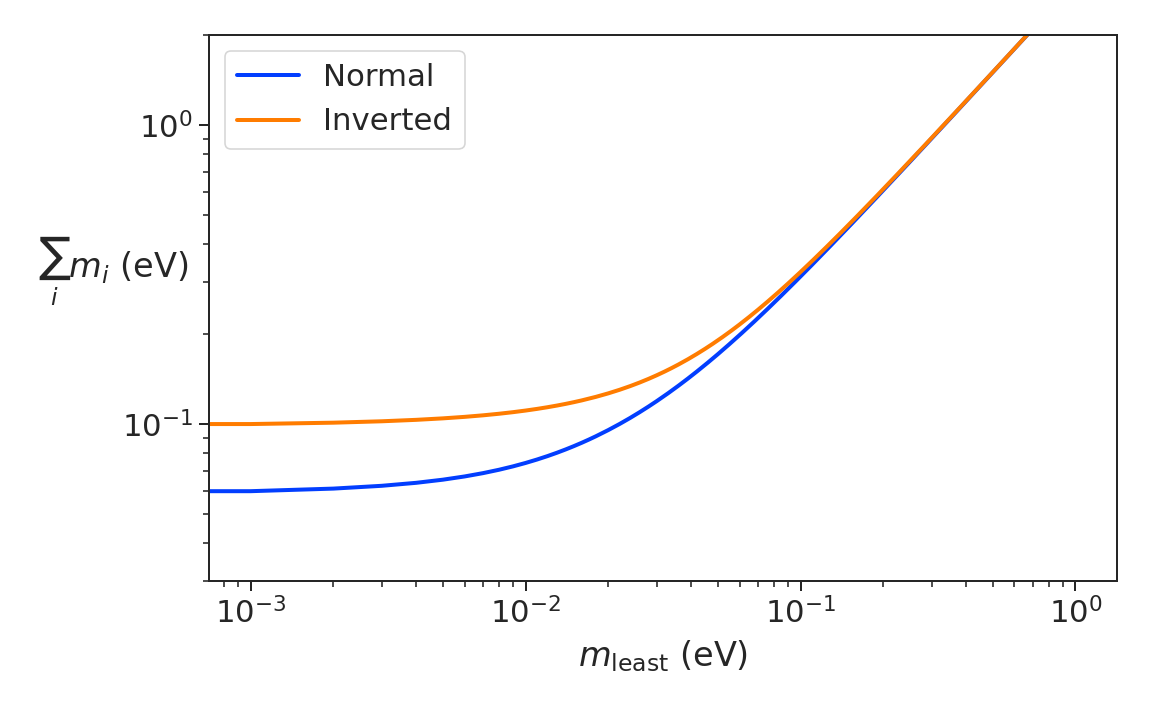
\includegraphics[width=0.7\textwidth]{figs/Chapter-2/230301_cosmology_nu_mass_observable.png}
    \caption{Caption}
    \label{fig:nu_mass_cosmo}
\end{figure}


%\begin{figure}[htbp]
%    \centering
%    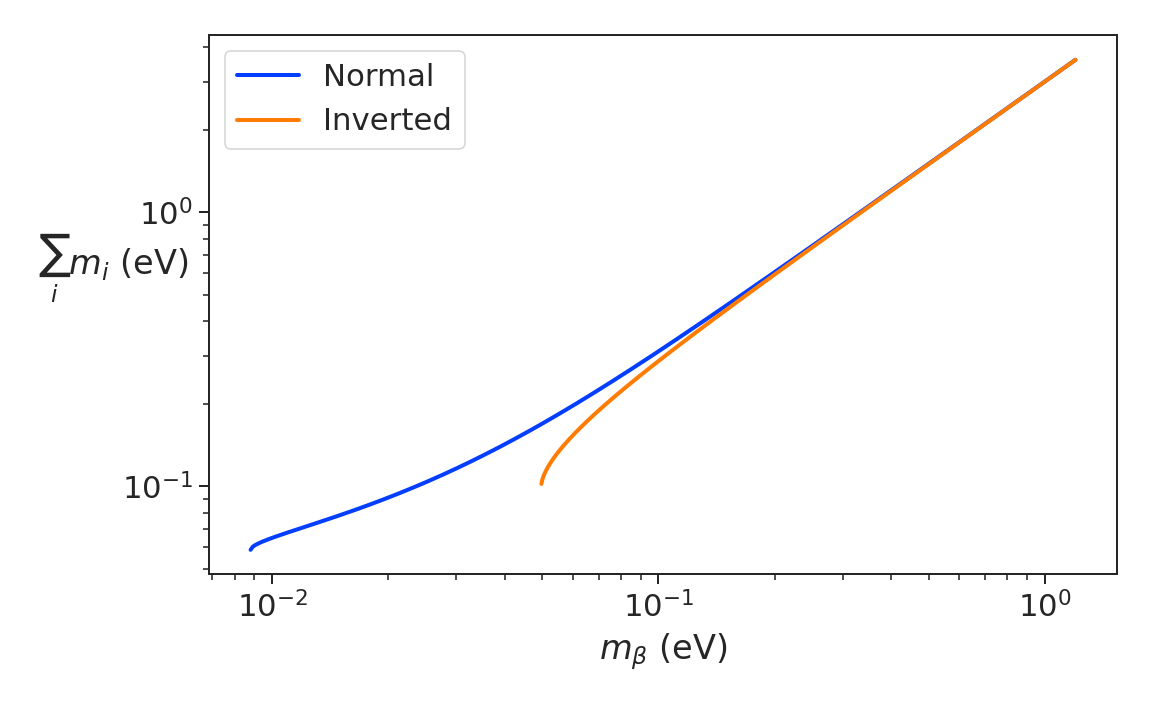
\includegraphics[width=0.7\textwidth]{figs/Chapter-2/230301_sum_nu_mass_vs_m_beta.png}
%    \caption{Caption}
%    \label{fig:nu_mass_cosmo_vs_nu_beta}
%\end{figure}
%\lipsum[1]

\subsection{Limits from Neutrinoless Double Beta-decay Searches}

\begin{figure}[htbp]
    \centering
    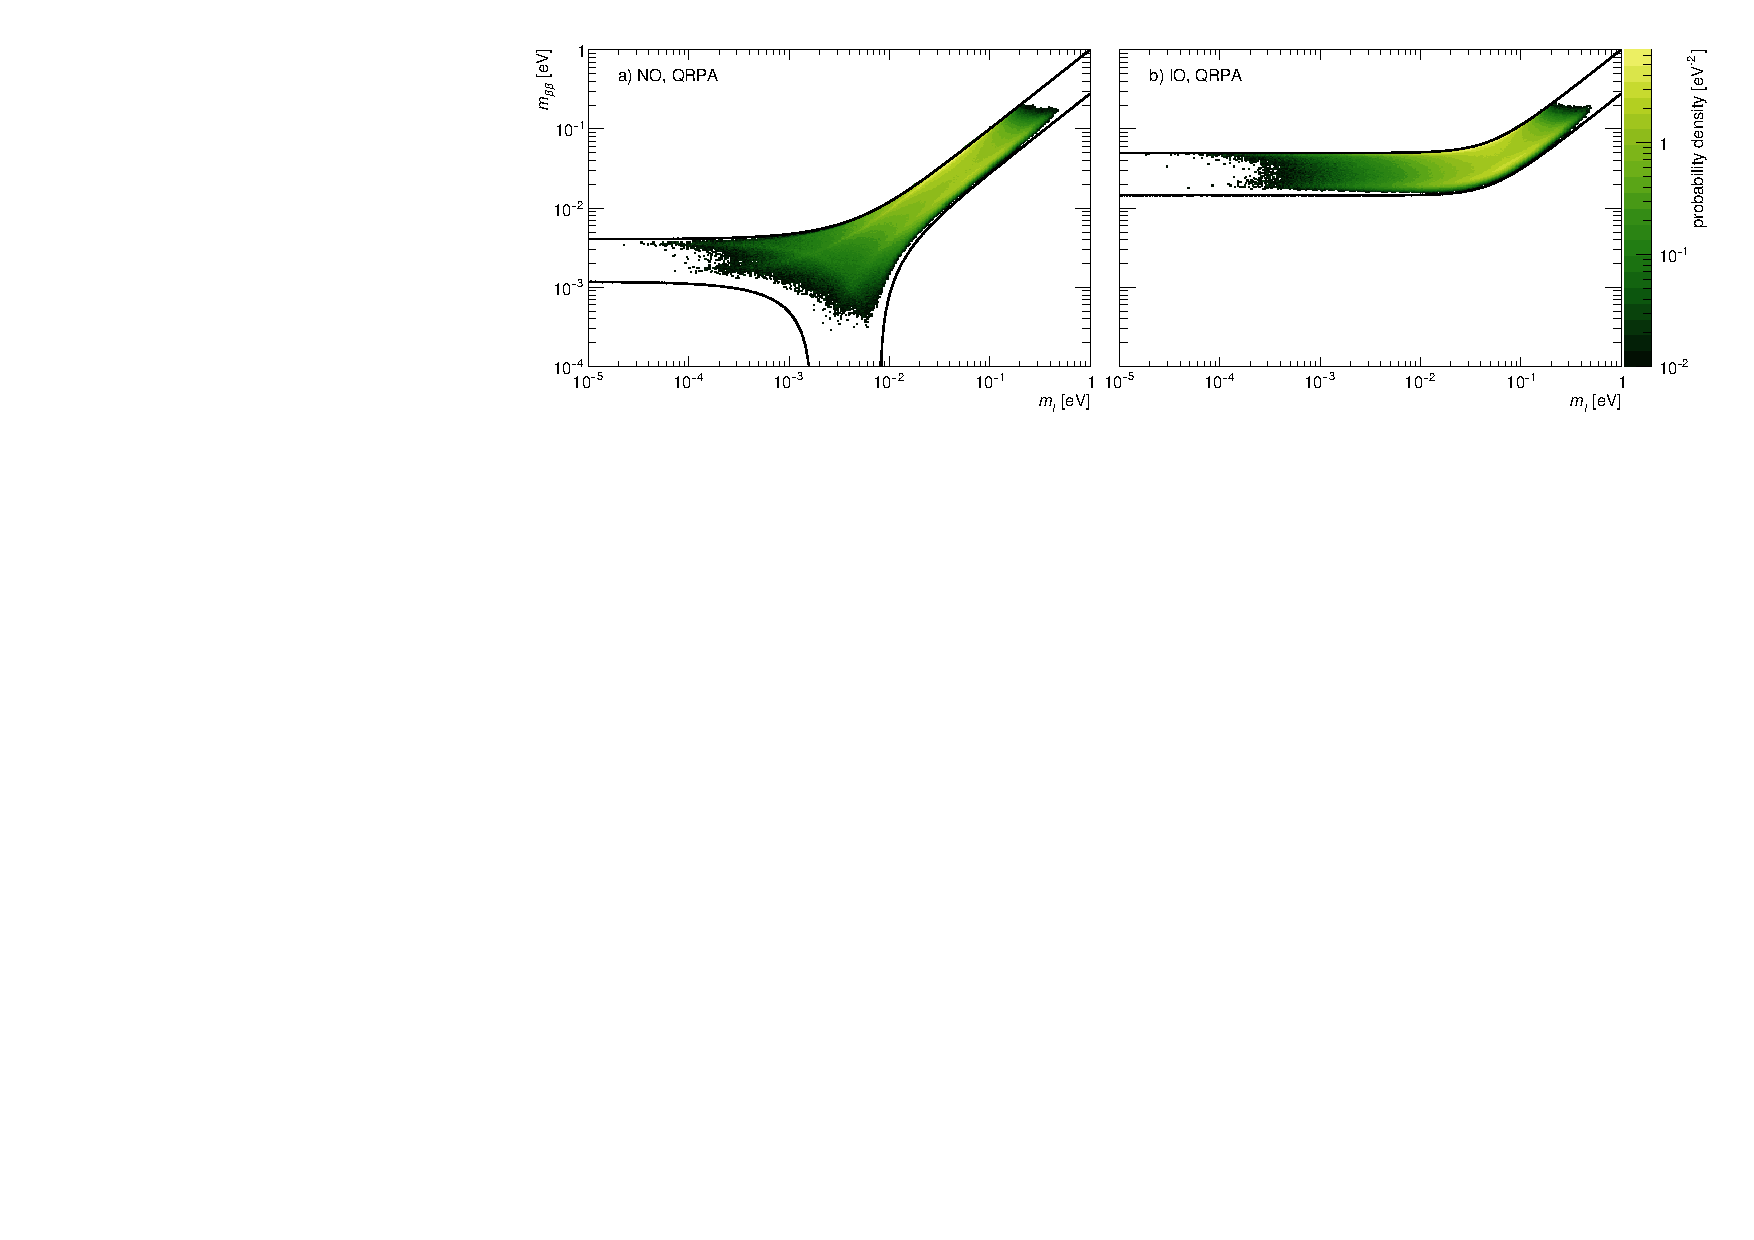
\includegraphics[width=1.0\textwidth]{figs/Chapter-2/230228_nu_mass_0nbb.pdf}
    \caption{Caption}
    \label{fig:nu_mass_0nbb_posterior}
\end{figure}

\begin{figure}[htbp]
    \centering
    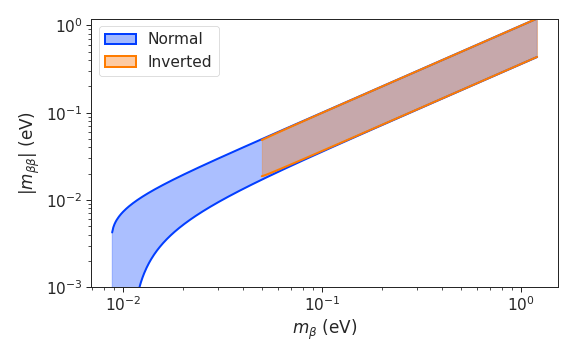
\includegraphics[width=0.7\textwidth]{figs/Chapter-2/230301_mbb_vs_mb.png}
    \caption{Caption}
    \label{fig:nu_mass_0nbb_vs_nu_beta}
\end{figure}

\subsection{Kinematic Measurements of the Neutrino Mass}

\begin{figure}[htbp]
    \centering
    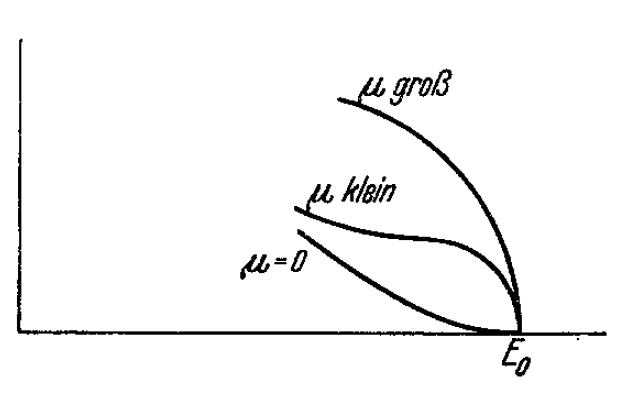
\includegraphics[width=0.7\textwidth]{figs/Chapter-2/Fermi.png}
    \caption{Caption}
    \label{fig:fermi_original_b_spectrum}
\end{figure}

\begin{figure}[htbp]
    \centering
    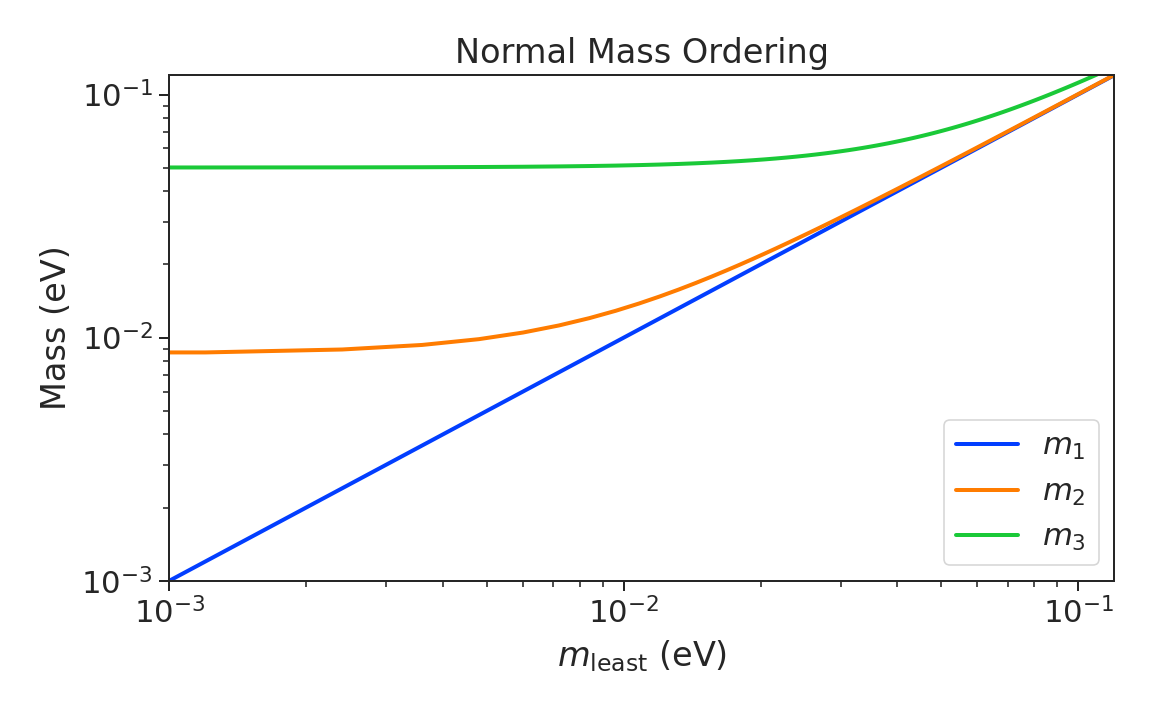
\includegraphics[width=0.7\textwidth]{figs/Chapter-2/230302_mass_estate_vals_normal.png}
    \caption{Caption}
    \label{fig:mass_estates_normal}
\end{figure}

\begin{figure}[htbp]
    \centering
    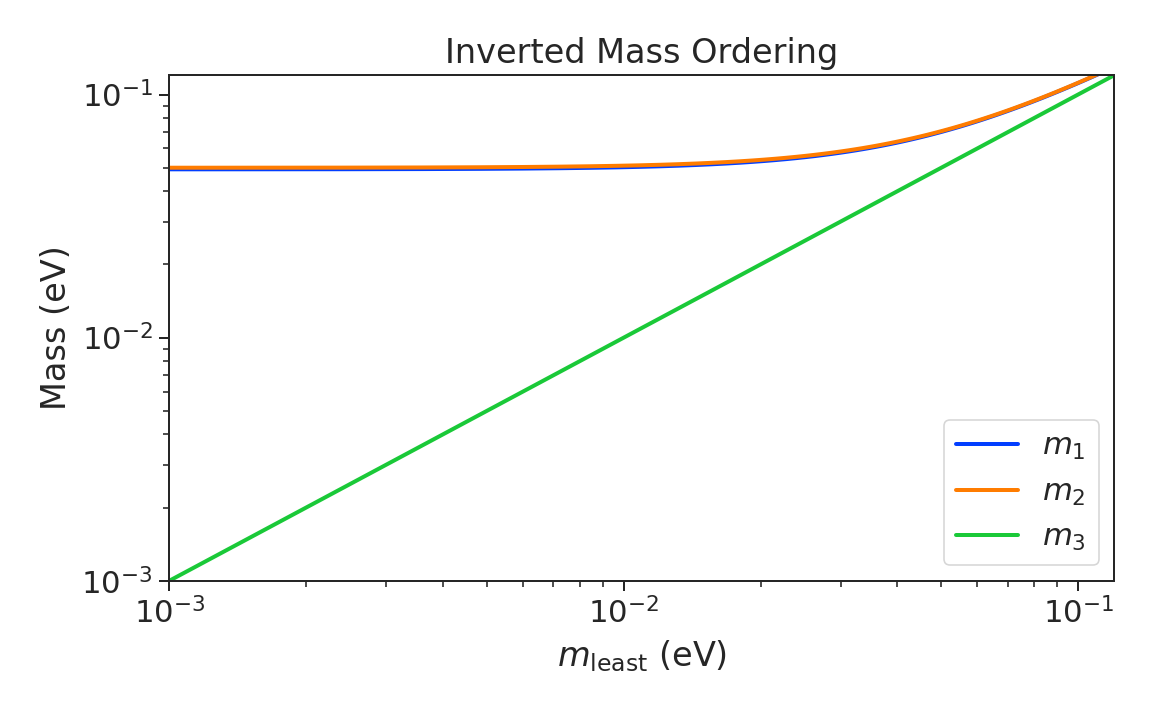
\includegraphics[width=0.7\textwidth]{figs/Chapter-2/230302_mass_estate_vals_inverted.png}
    \caption{Caption}
    \label{fig:mass_estates_inverted}
\end{figure}

\section{Neutrino Mass Measurements Using Tritium Beta-decay Spectroscopy}

\begin{figure}[htbp]
    \centering
    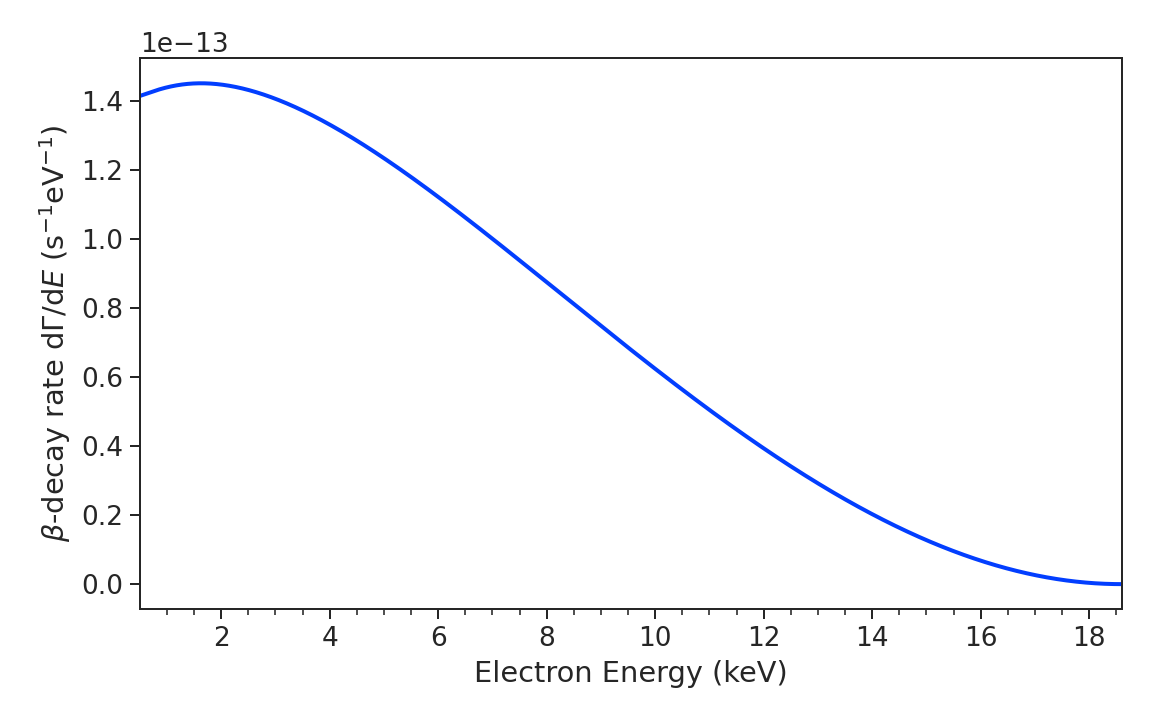
\includegraphics[width=0.7\textwidth]{figs/Chapter-2/230302_atomic_tritium_spectrum.png}
    \caption{Caption}
    \label{fig:atomic_tritium_spectrum}
\end{figure}

\begin{figure}[htbp]
    \centering
    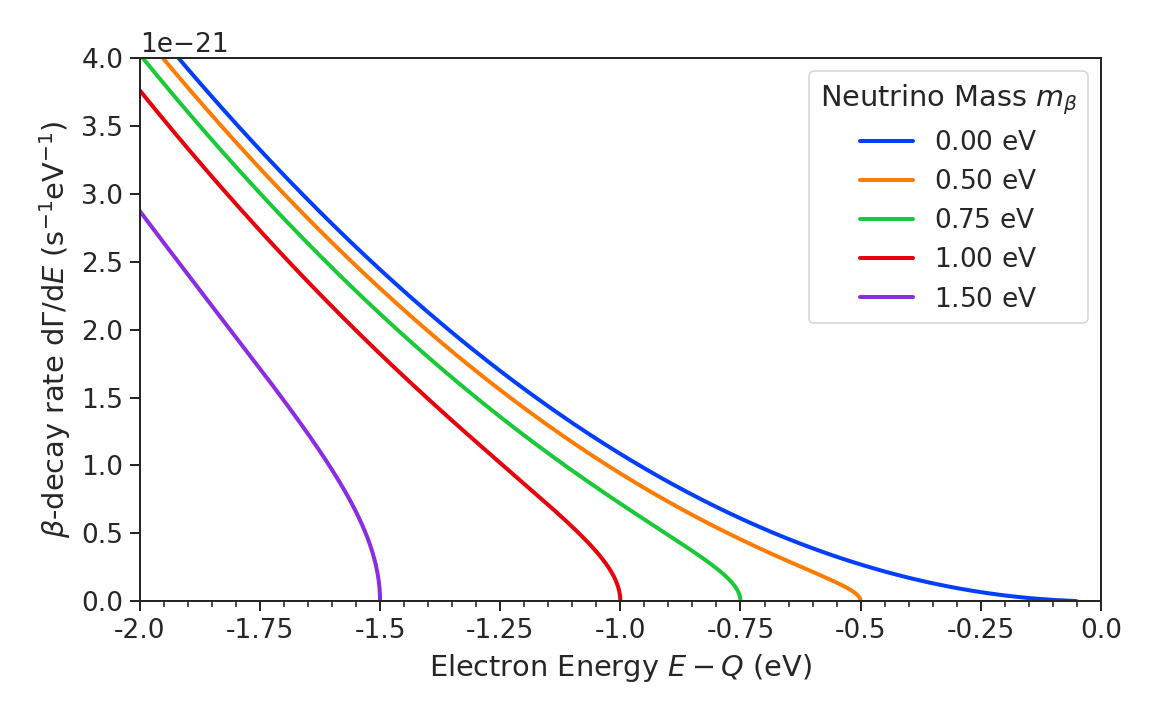
\includegraphics[width=0.7\textwidth]{figs/Chapter-2/230302_atomic_tritium_spectrum_near_endpoint.png}
    \caption{Caption}
    \label{fig:atomic_tritium_endpoint}
\end{figure}

% !TEX root = ../YourName-Dissertation.tex

\chapter{Direct Measurement of the Neutrino Mass with Project 8}

\section{Introduction}

A promising technique for direct measurements of the neutrino mass beyond the projected $200$~meV limit of the KATRIN experiment \cite{KATRIN:2022kkv} is tritium beta-decay spectroscopy with an atomic tritium source \cite{direct_meas_nu_mass}. Atomic tritium, combined with a large-volume, high-resolution energy measurement technique, is capable of measuring the neutrino mass with sensitivity below the 50~meV, which exhausts the range of neutrino masses allowed under the inverted hierarchy. 

Cyclotron Radiation Emission Spectroscopy (CRES) is a high-resolution energy measurement technique compatible with atomic tritium production and storage that can enable the next-generation of neutrino mass direct measurement experiments \cite{p8originalcres}. The Project 8 collaboration is currently engaged in a program of research and development (R\&D) aimed at developing the technology necessary for a measurement of the neutrino mass using CRES and atomic tritium with a sensitivity of 40~meV \cite{p8snowmass2022}.

In Section \ref{sec:chap3-cres-and-p8} I provide an introduction to the basics of the CRES technique as well as the goals of the Project 8 experiment. Additionally, I sketch out the phased experiment development plan being implemented by Project 8 to build towards a next-generation neutrino mass experiment.

In Section \ref{sec:chap3-phaseII} I give an overview of Phase II of the Project 8 experiment \cite{p8prc2023,p8prl2023}, which completed early in 2023. Although the bulk of the work presented in this dissertation is relevant to designs of future Project 8 experiments, a description of the work in Phase II provides useful context.

In Section \ref{sec:chap3-phaseIII-antenna-arrays} I introduce a CRES measurement concept based on antenna arrays \cite{p8jugaad}, which could be the basis for the ultimate Project 8 neutrino mass experiment. A significant portion of the R\&D efforts of Project 8 in Phase III were directed towards simulating and modeling this experimental concept in order to understand the achievable sensitivity to the neutrino mass.

Lastly, in Section \ref{sec:chap3-freq-choice-and-pilot-scale} I introduce conceptual designs of pilot-scale experiments and Phase IV that combine atomic CRES with a large-volume CRES detection technique. This includes a design concept for an antenna array based experiment, but also a design for a resonant cavity based experiment. Resonant cavities are discussed in more depth in Chapter \ref{chap:cavity} and have become the default choice for the Phase IV experiment.

\section{Project 8 and Cyclotron Radiation Emission Spectroscopy}
\label{sec:chap3-cres-and-p8}

\subsection{Cyclotron Radiation Emission Spectroscopy --- CRES}
\label{sec:chap3-cres}

Time and frequency are two of the most precisely measured quantities in physics. %It is often advantageous to convert measurements of other physical quantities like mass or length into frequency measurements due to the digital nature of frequency measurements that make them immune to many sources of noise. 
Atomic clocks, which operate by measuring the frequencies of various atomic transitions, have been used to measure time with astounding relative uncertainties of $10^{-18}$~seconds \cite{atomic_clock}. The extreme precision possible with frequency measurements is often summarized using the famous quote from the Physicist Arthur Schawlow who said advise his students to "Never measure anything but frequency!" \cite{never_meas_anything_but_freq}. 

Neutrino mass measurements using tritium beta-decay require the measurement of perturbations to the 18.6-keV tritium endpoint with a precision as small as 0.1~eV. Therefore, a spectroscopic technique with extremely high resolution is required. Frequency measurements are capable of such high-resolutions for the intuitive reason that they are essentially digital counting measurements, which average the number of oscillations of a physical system over time. By observing a rapidly oscillating system over a sufficient length of time one can obtain essentially arbitrary precision on a frequency limited only by the measurement time and signal-to-noise ratio (SNR) of the system.

A method is required for translating a kinetic energy measurement into a frequency measurement. A straightforward way to accomplish this is to place a gaseous supply of tritium into a magnetic field; therefore, when a beta-decay occurs the resulting electron will immediately begin to orbit around a magnetic field line at the cyclotron frequency, proportional to its kinetic energy (see Figure \ref{fig:chap3-cres-cartoon}). The acceleration caused by the orbit leads to the emission of cyclotron radiation that can be detected using an array of antennas or resonant cavity. The starting frequency of the radiation gives the electron's initial kinetic energy, which is used to build the beta-decay spectrum and measure the neutrino mass. The name for this measurement technique is Cyclotron Radiation Emission Spectroscopy or CRES \cite{p8originalcres}.

\begin{figure}[htbp]
    \centering
    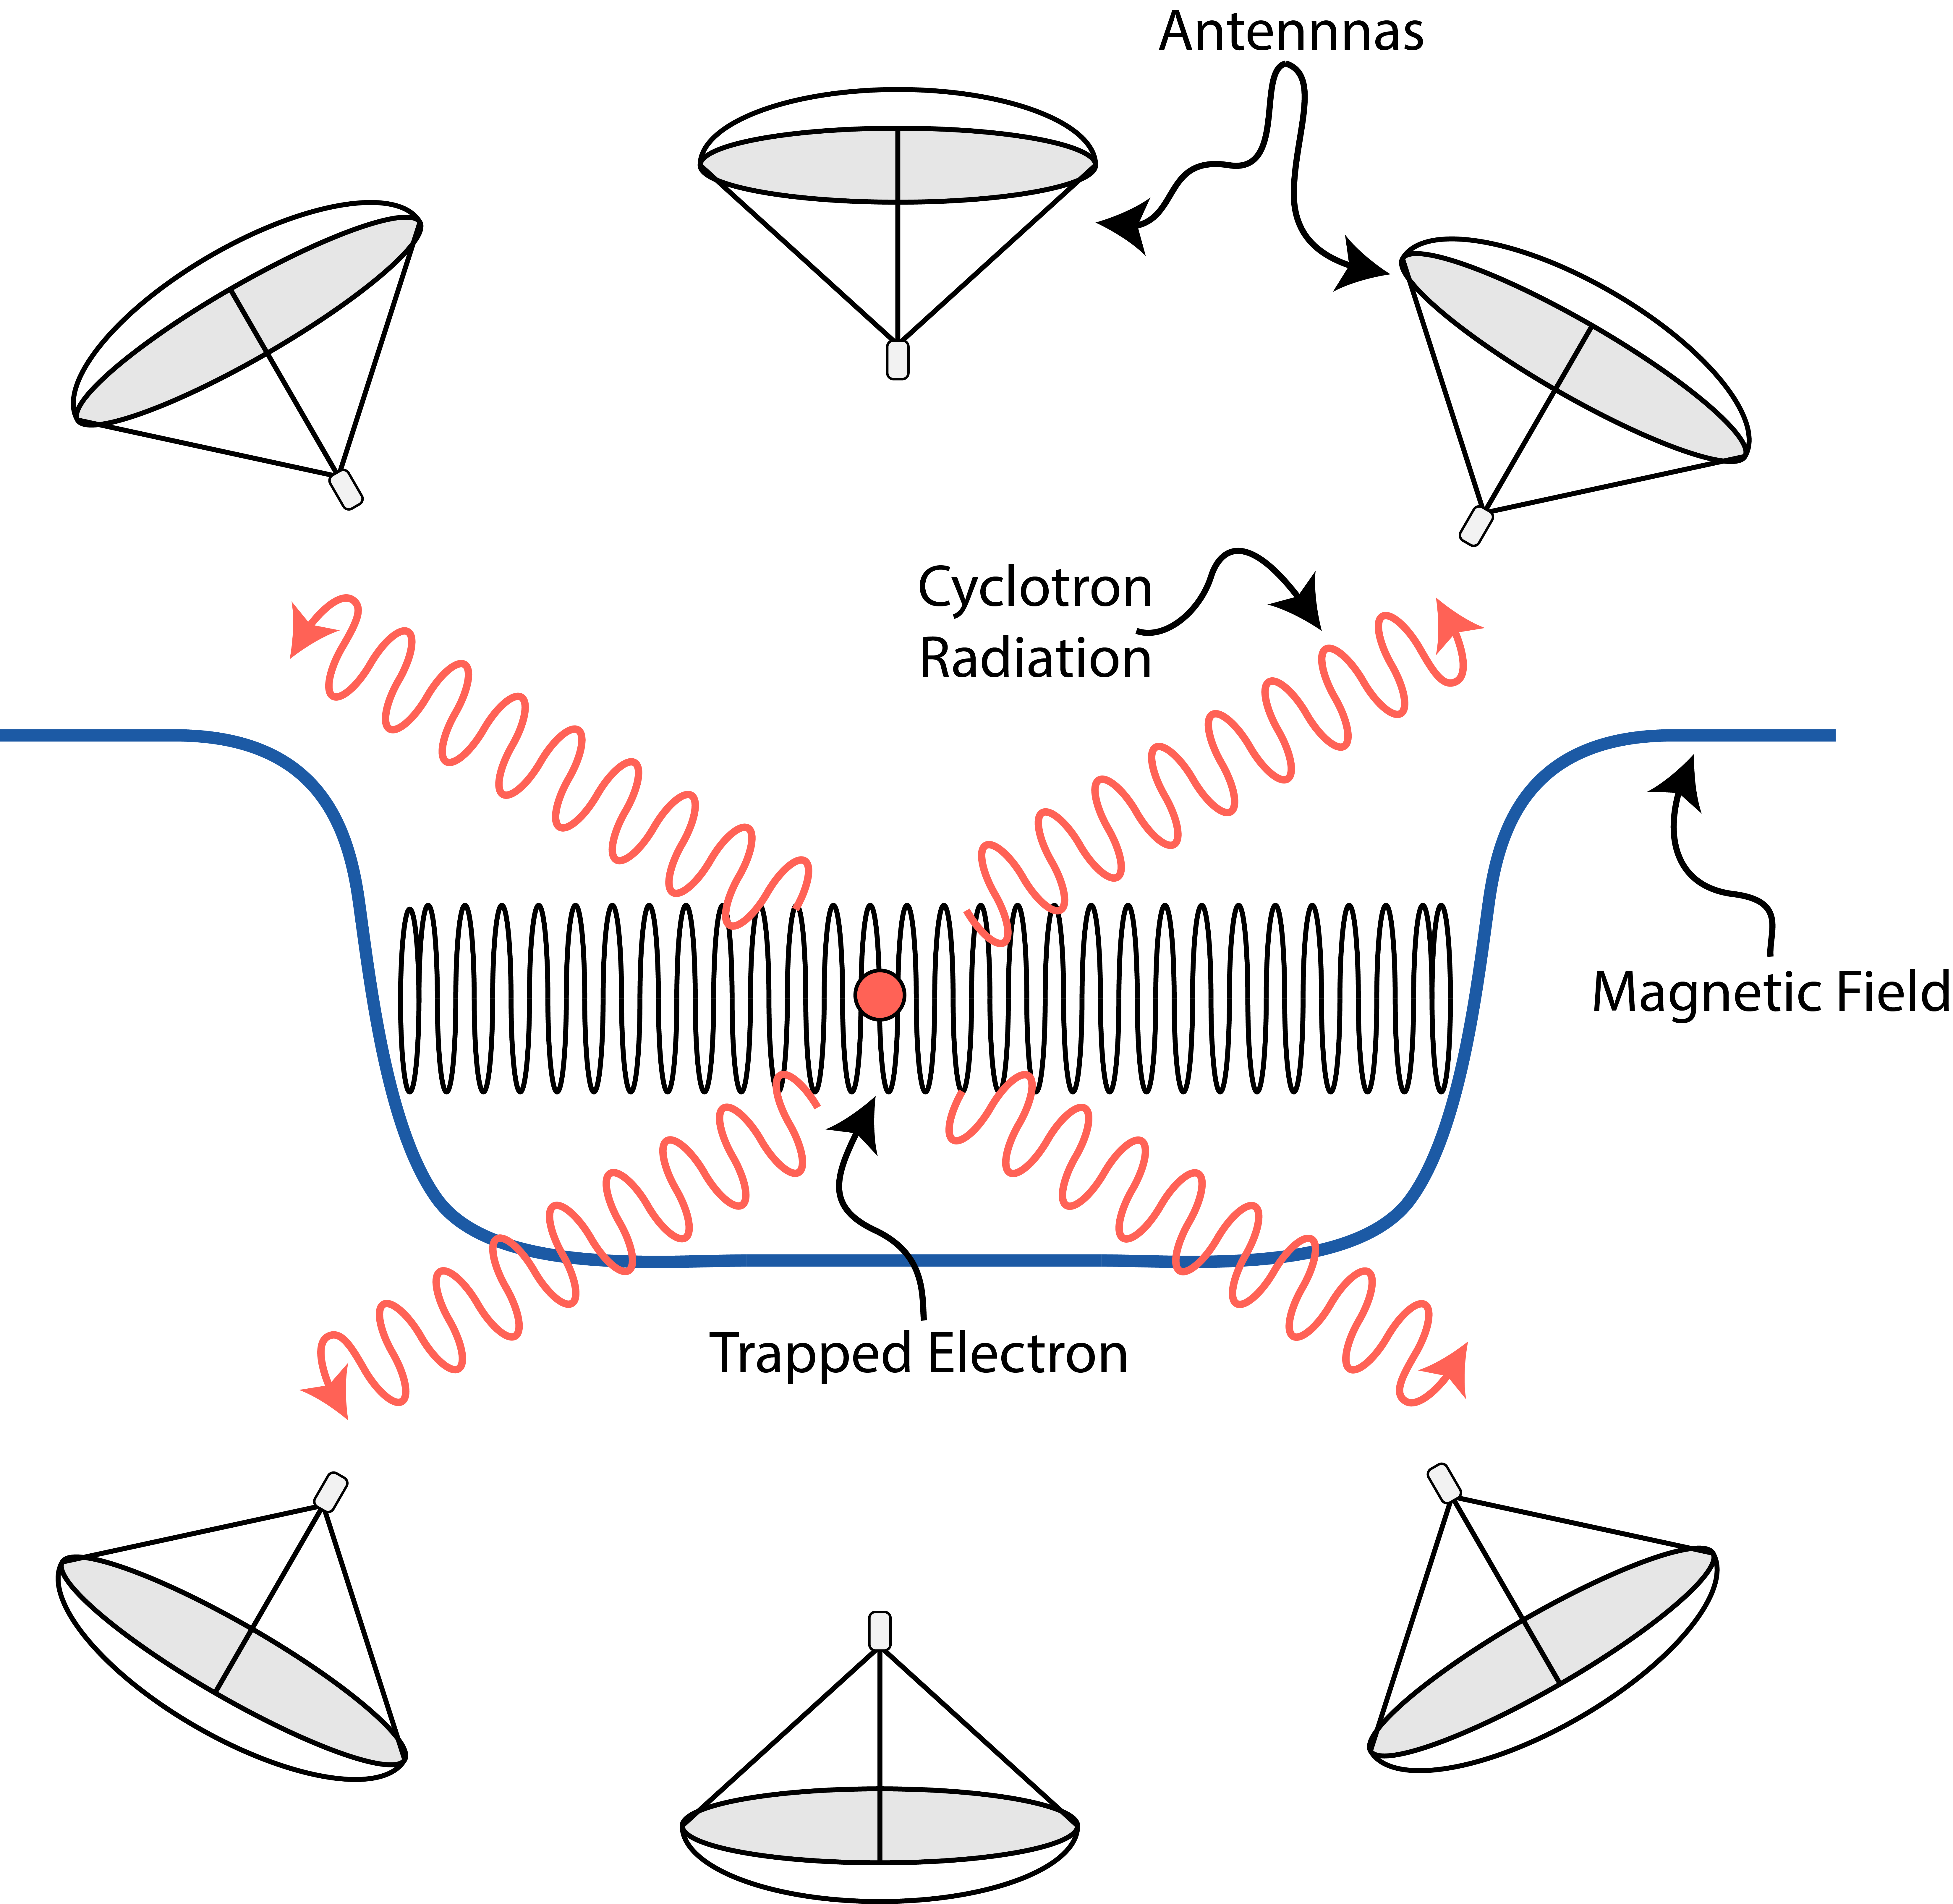
\includegraphics[width=0.5\textwidth]{figs/Chapter-3/230303_cres_cartoon.png}
    \caption{A cartoon illustration of the CRES technique. An electron is contained in a magnetic trap, which is a local minimum in the magnetic field, so that its cyclotron radiation can be detected by an array of antennas. Detecting the cyclotron radiation allows one to measure its cyclotron frequency and determine its kinetic energy.}
    \label{fig:chap3-cres-cartoon}
\end{figure}

In the non-relativistic case, the cyclotron frequency is simply a function of the charge-to-mass ratio of the particle; however, the relativistic correction to the cyclotron frequency
\begin{equation}
    f_c = \frac{qB}{2\pi m_e\gamma}=\frac{1}{2\pi}\frac{qB}{m_e+E_\mathrm{kin}/c^2},
    \label{eq:chap3-cyclotron-freq}
\end{equation} 
introduces a dependence of the kinetic energy ($E_\mathrm{kin}$) to the inverse of the cyclotron frequency ($f_c$). Electrons with kinetic energies of 18.6~keV are in the weakly relativistic regime with $\beta=\frac{v}{c}=0.263$ and $\gamma=1.036$.

The frequency resolution of a CRES measurement can be estimated by differentiating Equation \ref{eq:chap3-cyclotron-freq},
\begin{equation}
    \frac{df_c}{dE_\mathrm{kin}} = \frac{1}{2\pi}\frac{-qBc^2}{\left(m_ec^2+E_\mathrm{kin}\right)^2},
\end{equation}
from which one obtains the relationship between fractional differences in energy and frequency,
\begin{equation}
    \frac{df_c}{f_c}=\frac{1-\gamma}{\gamma}\frac{dE_\mathrm{kin}}{E_\mathrm{kin}}.
\end{equation}
Therefore, an energy precision of 1~eV for an 18.6~keV electron can be achieved with a frequency precision of approximately 2~ppm.

The minimum observation time required to achieve this resolution can be estimated using the uncertainty principle as formulated by Gabor \cite{gabor}. Electrons from tritium beta-decay experience random collisions with the background gas particles, which limits the uninterrupted radiation lifetime. The time between collision events, referred to as "track length", is an exponentially distributed variable. Differences in the track lengths of a population of mono-energetic electrons leads to an uncertainty or broadening in the distribution of measured frequencies, which is proportional to the mean track length, $\tau_\lambda$. The resulting frequency distribution has a Lorentizan profile, whose width is given by the Gabor limit,
\begin{equation}
    \tau_\lambda\Delta f_c=\frac{1}{2\pi}\implies\Delta f_c=\frac{1}{2\pi\tau_\lambda}.
\end{equation}
The cyclotron frequency for a 18.6-keV electron in a 1~T field is approximately 27~GHz, consequently, the minimum observation time for a frequency resolution of 2~ppm is approximately 3~$\mu$sec. 

Strictly speaking, the Gabor limit is not the true lower bound on the frequency resolution for a CRES signal, since it derives from the Fourier representation of a fixed length time-series using a basis of infinite duration sinusoids. If one takes the approach of fitting the CRES signal in the time-domain, then the lower limit on frequency precision is given by the Cram\'{e}r-Rao lower bound (CRLB) \cite{nick_viterbi}, which depends on the track length and SNR. The CRLB is the minimum variance achievable by an unbiased estimator for an unknown but deterministic parameter, and, in general, the CRLB allows for better precision on the cyclotron frequency.

\begin{figure}[htbp]
    \centering
    \includegraphics*[width=0.75\textwidth]{figs/Chapter-3/230628_bathtub_trap.png}
    \caption{\label{fig:chap3-bathtub-trap}An illustration of an electron in a bathtub magnetic trap generated by two well-separated coils.}
\end{figure}

Ensuring that an electron remains under observation long enough so that its frequency can be precisely measured requires a magnetic trap. A magnetic trap is a local minimum in a background magnetic field generated an appropriate configuration of electromagnetic coils. Since magnetic fields can do no work, there is no danger of the magnetic trap affecting the kinetic energy of the electron after it is emitted from the beta-decay. One common approach to creating a magnetic trap is the "bathtub" trap configuration, which can be produced using two magnetic pinch coils aligned on a central axis that are separated by a distance that is large compared to the coil radius (see Figure \ref{fig:chap3-bathtub-trap}). This configuration produces a trap with a uniform bottom and relatively steep walls, which is ideal for CRES measurements. 

The electron's pitch angle is a useful parameter for describing its motion in the magnetic trap. Pitch angle is defined in terms of the ratio between the component of the electron's velocity perpendicular to the magnetic field and the component parallel to the magnetic field
\begin{equation}
    \tan{\theta_p}=\frac{v_\perp}{v_\parallel}.
\end{equation}
Electrons with pitch angles less than $90^\circ$ oscillate back and forth in the magnetic trap, which leads to variations in the cyclotron frequency caused by the changing value of the magnetic field along the electron's path. This leads to frequency modulation that produces sidebands in the cyclotron radiation spectrum. Resolving these sideband frequency components is necessary for a complete reconstruction of the CRES signal in the experiment.

Electrons trapped in a cylindrically symmetric trap have three primary components of motion (see Figure \ref{fig:chap3-trapped-electron-motion}).
\begin{figure}[htbp]
    \centering
    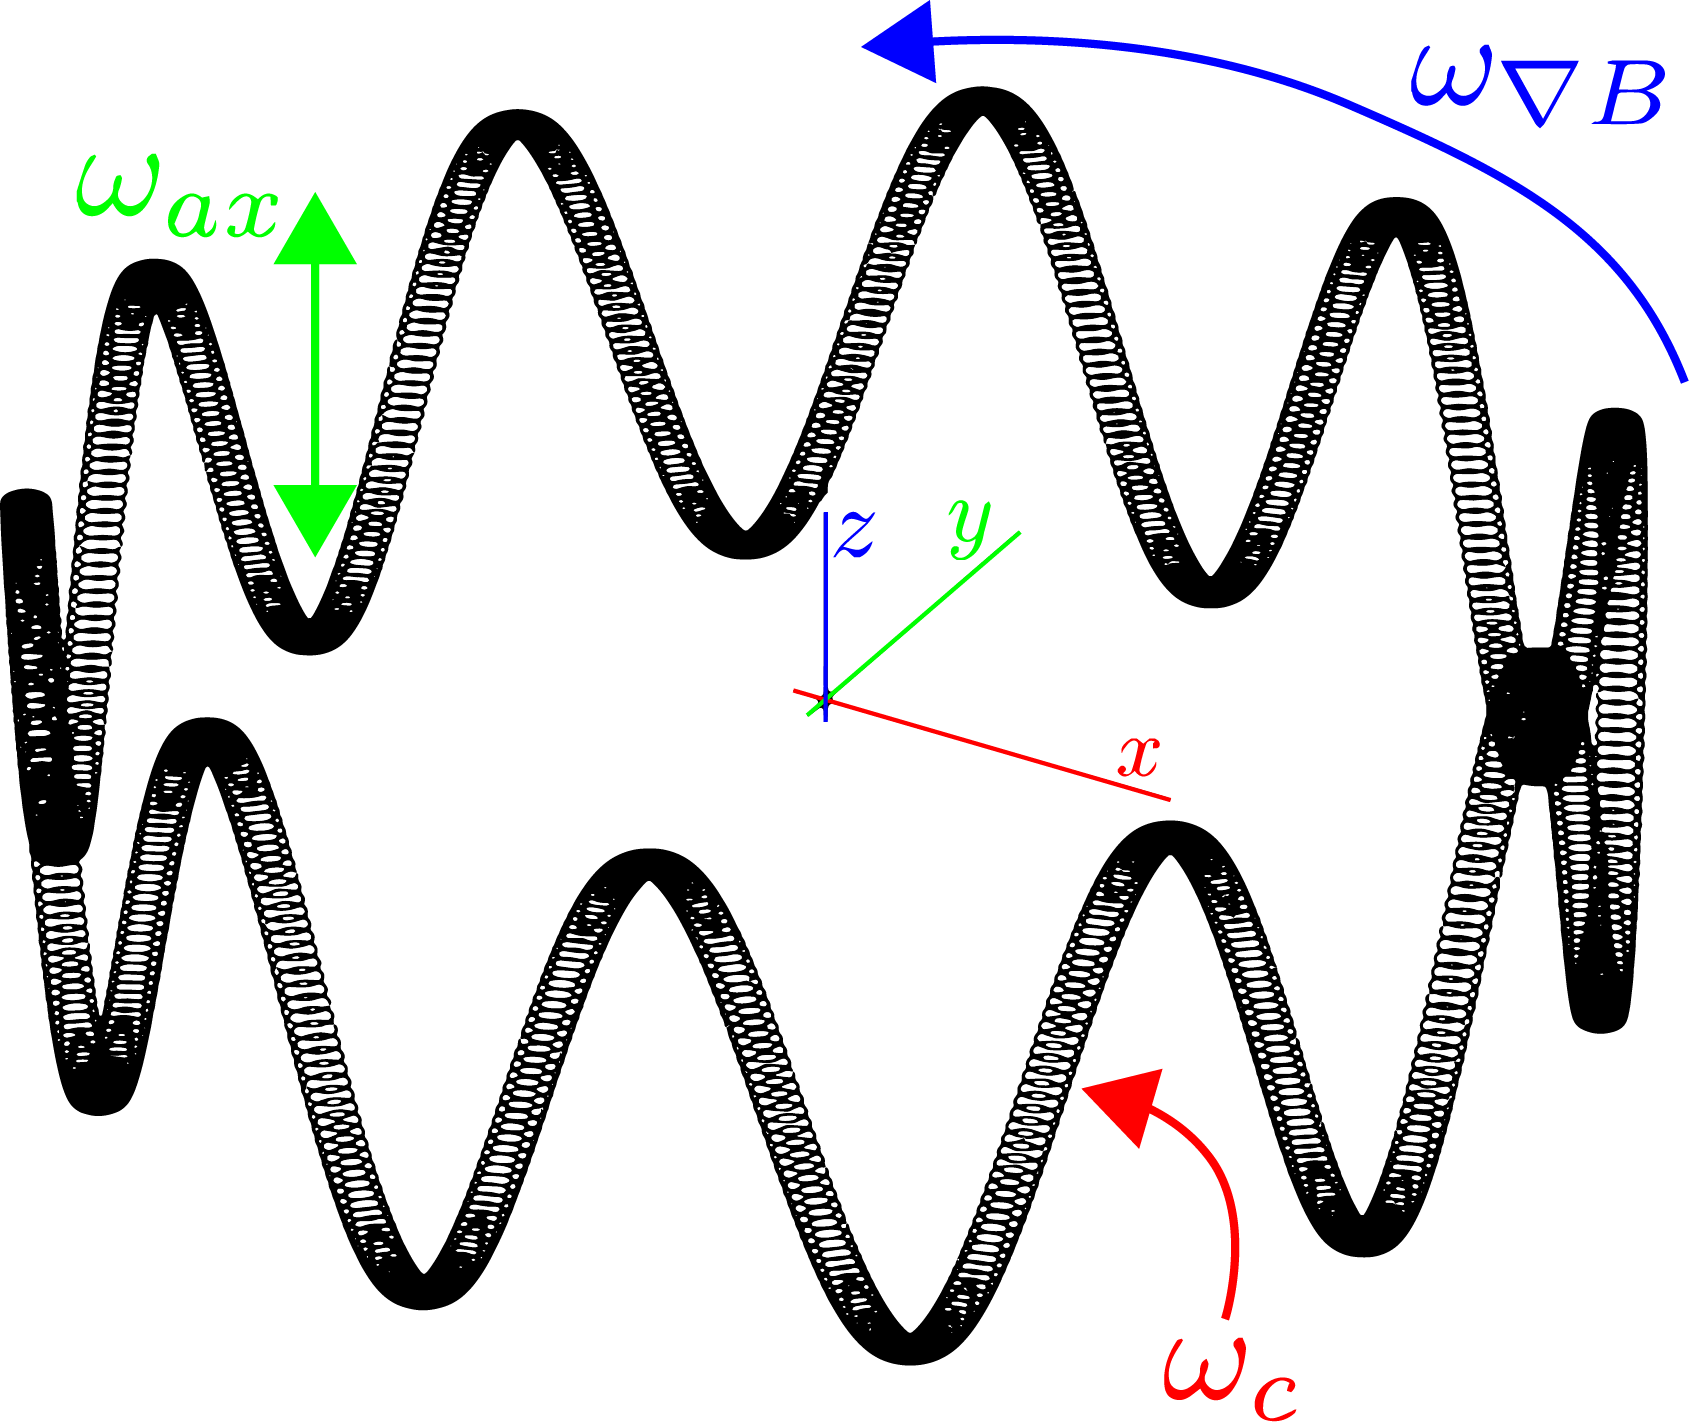
\includegraphics[width=0.5\textwidth]{figs/Chapter-3/230511_trapped_motion.png}
    \caption{A plot of the main components of an electron's trajectory in a cylindrically symmetric trap.}
    \label{fig:chap3-trapped-electron-motion}
\end{figure}
The dominant component, typically with the highest frequency, is the electron's cyclotron orbit, which encodes information on the electron's kinetic energy. Axial motion from the electron's pitch angle leads to frequency modulation, and a shift in the average magnetic field experienced by an electron. This leads to a correlation between the kinetic energy of the electron and the pitch angle depending on the particular shape of the magnetic trap, which can negatively impact energy resolution. Generally, more variation in the magnetic field along the electron's trajectory leads to a worse energy resolution. The magnetic trap can be engineered to have a flat bottom with very steep walls to mitigate this effect. A bathtub trap design, where the distance between the coils is much greater than the coil radius, is the trap that best approximates this ideal design. Radial gradients in the trap leads to a third component of motion called grad-B drift \cite{jackson_classical_1999}. The equation for the drift velocity is
\begin{equation}
    \mathbf{v}_{\nabla B} = \frac{m_e v_\perp^2}{2qB}\frac{\mathbf{B}\times\nabla B}{B^2}.
\end{equation}
%These additional components of motion all influence the shape of the CRES signal so modeling their effects is critical to proper measurement of the kinetic energy.

The total power of the radiation emitted by an electron in a free-space environment is given by the Larmor equation \cite{larmor_eqn}
\begin{equation}
    P(\gamma, \theta_p)=\frac{1}{4\pi\epsilon_0}\frac{2}{3}\frac{q^2\omega_c^2}{c}(\gamma^2 - 1)\sin^2{\theta_p},
\end{equation}
where $\omega_c$ is the cyclotron frequency multiplied by $2\pi$ and $\theta_p$ is the pitch angle to distinguish it from the spherical angle coordinate. A single electron with a $90^\circ$ pitch angle and 18.6~keV of kinetic energy in a 1~T magnetic field emits a total radiation power of 1.2~fW. Furthermore, one is typically only able to receive a fraction of this total power with an antenna or other detection system. Therefore, RF (radio-frequency) systems in CRES experiments must be operated at cyrogenic temperatures to limit the noise power such that adequate SNR can be achieved for signal detection and reconstruction. Alternatively, longer tracks enable detection of weaker signals due to the increase in the total signal energy available for the detection algorithm.

\subsection{Project 8}

The Project 8 collaboration\footnote{\url{https://www.project8.org/}} is a group of institutions in the United States and Germany building an experiment to measure the neutrino mass by developing a novel spectrometer technology based on CRES. In the ultimate Project 8 experiment, the CRES technique will be used to measure the beta-decay spectrum using a large source of atomic tritium sufficient to achieve the required statistics in the last $O(10)$~eV of the decay spectrum. Project 8 is targeting a neutrino mass sensitivity below 50~meV \cite{p8snomass}, which exhausts the range of possible neutrino masses under the inverted hierarchy and is a factor of four less than sensitivity projections for the ongoing KATRIN experiment.

Project 8's proposed experiment requires the development of two novel technologies: the production and trapping of a source of atomic tritium on cubic-meter scales and technology to enable CRES measurements of individual electrons in the same volume. 

\subsubsection*{Atomic Tritium}

Previous measurements of the tritium beta-decay spectrum for neutrino mass measurements have relied on  sources of molecular tritium for their measurements \cite{mainz_final,troitsk_result,KATRIN:2022kkv} due to the technical challenges associated with the production and storage of atomic tritium.

\begin{figure}[htbp]
    \centering
    \includegraphics*[width=0.5\textwidth]{figs/Chapter-3/atmol2.pdf}
    \caption{\label{fig:chap3-atomic-vs-mol-final-state-spectra} A plot of the final state distributions of atomic and molecular tritium. The final state distribution provides the primary contribution to the width of the molecular spectrum whereas thermal doppler broadening is responsible for the width of the atomic spectrum.}
\end{figure}

One must supply sufficient energy to the tritium molecules to break the molecular bond and create atomic tritium. Common approaches include the use of hot coaxial filament atom crackers as well as plasma sources. Both involve heating the tritium atoms to temperatures of $>2500$~K, which must then be cooled to temperatures on the order of a few~mK so that the tritium atoms can be trapped. Cooling the atoms requires the construction of a large tritium infrastructure and cooling system that can supply a source of cold atoms to the trap. 

Once cold tritium atoms are produced they cannot make contact with any surfaces to avoid recombination of the atoms to molecules. Therefore, a magnetic trap is required to store the atoms for a sufficient length of time that they have a chance to decay before escaping the trap. Trapping the atoms requires the construction of a large and complex magnet system that must be cooled to cryogenic temperatures.

The significant experimental complexity caused by atomic tritium makes a molecular source the obvious choice from practical considerations. However, the drawback of molecular tritium for neutrino mass measurement is the irreducible broadening in the electron's kinetic energy due to the final state spectrum of molecular tritium (see Figure \ref{fig:chap3-atomic-vs-mol-final-state-spectra}). The broadening of the final state spectra has a RMS amplitude of 436~meV \cite{tritium_final_state_saenz, Bodine:2015sma} caused by variation in the final vibrational state of the daughter molecule.

For atomic tritium, the primary sources of broadening in the final state spectrum are magnetic hyperfine splittings (magnitude of $O(10^{-5})$~eV) and thermal Doppler broadening caused by the motion of the trapped atom. Atomic tritium at a temperature of 1~mK has an energy broadening dominated by thermal Doppler component, providing about 1~meV RMS of broadening to the electron's kinetic energy.

The larger energy broadening with molecular tritium leads to an irreducible statistical uncertainty that limits the achievable sensitivity to approximately 100~meV at 90\% confidence. For previous direct measurements of the neutrino mass, this uncertainty is an insignificant contribution to the overall uncertainty budget. However, for experiments like Project 8 atomic tritium will become a key component to the success of the final experiment.

\subsubsection*{CRES for Neutrino Mass Measurement}

Several features of the CRES technique make it an attractive choice for a next generation neutrino mass measurement experiment. Because CRES is a remote-sensing technique, it is possible to observe the kinetic energy of the electron without altering its trajectory or directly interacting with the particle; therefore, in a CRES experiment the source gas volume can be the same as the CRES spectrometer volume. Tritium gas is also transparent to cyclotron radiation, which means that the kinetic energies of electrons can be measured using a cavity or antenna array, located directly outside the atom trapping volume. 

Because source and spectrometer can be colocated, CRES experiments have an advantageous scaling law relative to the current state-of-the-art beta-decay spectroscopy experiment, KATRIN. KATRIN utilizes the magnetic adiabatic collimation with an electrostatic filter (MAC-E filter) technique to measure the beta-decay spectrum of molecular tritium. In this approach, a source of molecular tritium is located outside the spectrometer. When a beta-decay occurs the electron is guided out of the tritium source using a magnetic field and is transported through the MAC-E filter before it is detected on the other side of the filter using a charge sensor. The measurement statistics of the MAC-E filter are limited by the transverse area ($L^2$) of the tritium source and filter due to the need to travel through the experiment without scattering. This scaling is less favorable than the volumetric scaling ($L^3$) of CRES due to the ability to colocate source and detector.

Another promising aspect of the CRES technique is the inherently high precision of frequency based measurements. The endpoint of the molecular tritium beta-decay spectrum is approximately 18.6~keV, which dwarfs the neutrino mass scale of $<1$~eV/$\rm{c}^2$ by at least a factor of $10^5$. Measuring the effect of such a small mass on a high energy electron requires excellent energy resolution. Since frequency measurements are essentially counting measurements, they are intrinsically accurate due to the ability to measure the cyclotron frequency by effectively averaging over millions of cyclotron orbits. It is possible to achieve part-per-million accuracy on the kinetic energy with the CRES technique using the off-the-shelf RF components.

CRES is also nearly immune to typical sources of backgrounds that can plague other experiments. Since CRES operates via a non-destructive measurement of the electron's cyclotron frequency, sources of background electrons are effectively filtered out by limiting the frequency bandwidth of the measurement. The fiducial volume of the experiment is free from any surfaces that could introduce stray electrons, and electrons from sources outside the fiducial volume can be prevented from entering the experiment.

\subsubsection*{Neutrino Mass Sensitivity Goals}

Project 8's ultimate goal is to combine CRES with atomic tritium to measure the neutrino mass with 40~meV sensitivity at the 90\% confidence level (see Figure \ref{fig:chap3-p8-nu-mass-goal}).
\begin{figure}[htbp]
    \centering
    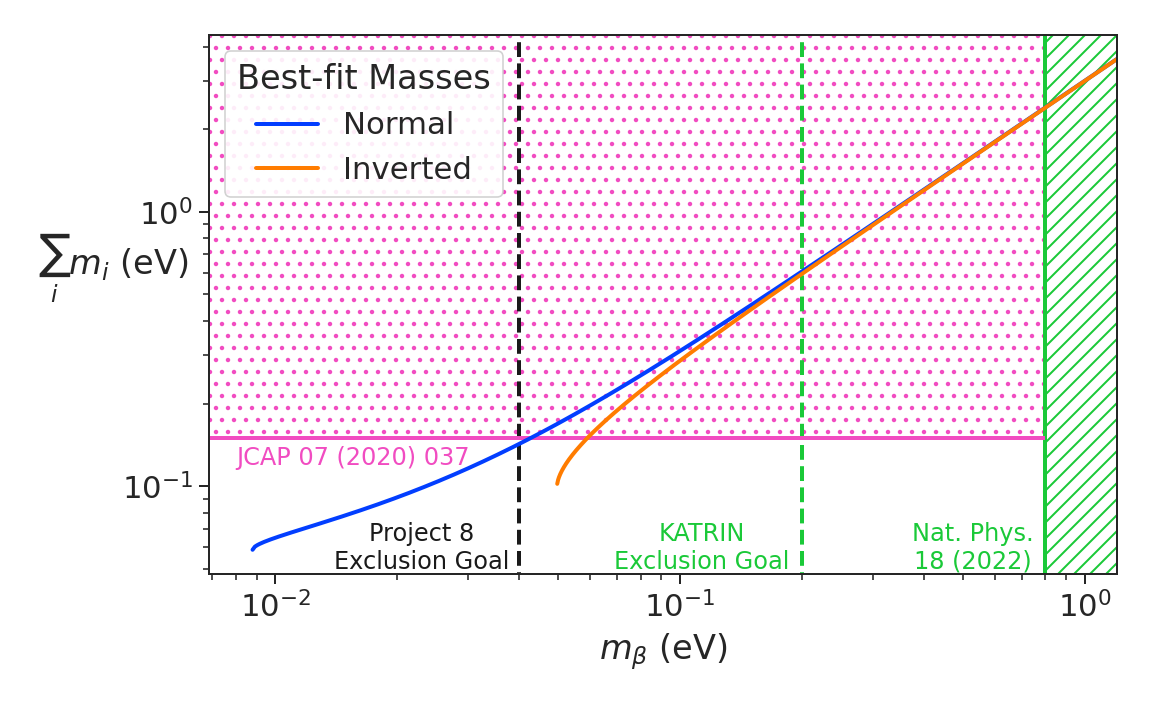
\includegraphics[width=0.7\textwidth]{figs/Chapter-3/230303_sum_nu_mass_vs_m_beta_with_exclusion_and_goal.png}
    \caption{Neutrino mass exclusion plot including limits from cosmological measurements and the KATRIN experiment. Allowed ranges for neutrino masses under the normal and inverted hierarchies are shown as the blue and orange lines respectively. The black dashed line shows Project 8's goal neutrino mass sensitivity for the Phase IV experiment.}
    \label{fig:chap3-p8-nu-mass-goal}
\end{figure}
This sensitivity is sufficient to fully exhaust the range of allowable neutrino masses under the inverted neutrino mass ordering regime and is approximately an order of magnitude less than the projected final sensitivity of the KATRIN experiment. Excluding the full neutrino mass parameter space would require a sensitivity an order of magnitude lower than what is proposed by Project 8, which would require an experiment whose size and complexity are currently well beyond proposals for the next-generation of neutrino mass direct measurement experiments.

\subsection{The Project 8 Phased Development Plan}

Reaching 40~meV sensitivity requires the simultaneous development and eventually combination of CRES and atomic tritium.
\begin{figure}[htbp]
    \centering
    \begin{subfigure}{0.725\textwidth}
        \includegraphics*[width=\textwidth]{figs/Chapter-3/sensitivity_vs_exposure_curve.pdf}
    \end{subfigure}
    \begin{subfigure}{0.67\textwidth}
        \includegraphics*[width=\textwidth]{figs/Chapter-3/sensitivity_vs_density_curve.pdf}
    \end{subfigure}
    \caption{Sensitivity calculations for a cavity based CRES experiment that demonstrate the neutrino mass measurement goals of Project 8 throughout the phased development plan. The blue curves indicate molecular tritium sources and the red curves indicate atomic tritium sources. In the current plan, Phase III contains two tritium experiments. The first is the Low-frequency Apparatus (LFA), which is a molecular tritium experiment, and the second is the atomic tritium pilot-scale experiment that officially ends Phase III. The sensitivity of these experiments is primarily a function of statistics; however, there is a critical density beyond which CRES electrons do not have enough time to radiate between collisions for a high-resolution frequency measurement leading to worse sensitivity. }
    \label{fig:chap3-sensitivity-calculations}
\end{figure}
These technologies require a significant up-front R\&D investment to build-out the required capabilities for a 40~meV CRES experiment. Therefore, Project 8 is following a phased experiment plan in which incremental progress can be made towards the ultimate goal of a 40~meV neutrino mass measurement with CRES (see Figure \ref{fig:chap3-sensitivity-calculations}).

Project 8's experiment plan is divided into four phases. The first phase, called Phase I, consisted of a demonstration of the CRES technique and a measurement of the internal conversion spectrum of $^{83m}$Kr. Phase II was the first measurement of the tritium beta-decay spectrum and neutrino mass measurement with CRES. Currently, Project 8 is engaged in Phase III, which is R\&D towards a scalable CRES measurement technique and atomic tritium source for the final Project 8 experiment in Phase IV. Phase IV is the ultimate experiment by Project 8 that will combine CRES with atomic tritium to measure the neutrino mass with a sensitivity of 40~meV. 

\subsubsection*{Phase I and II: Proof of Principle and First Tritium Measurements}

The earlier phases of the Project 8 experiment, Phase I and II, were focused on demonstration and development of the CRES technique itself as well as a proof-of-principle measurement of the neutrino mass using the CRES technique.

In Phase I, Project 8 performed a proof-of-principle measurement of the $^{83m}\rm{Kr}$ spectrum using CRES, which marked the first ever kinetic energy spectrum measurement with CRES. The experiment included all the components of a basic CRES experiment. An electron source consisting of a gas of $^{83m}\rm{Kr}$ was supplied to a waveguide gas cell constructed out of a segment of WR-42 waveguide and sealed with Kapton windows at the top and bottom. A magnetic trapping region was created in the waveguide cell using a single electromagnetic coil wrapped around the waveguide which provided a trapping volume on the order of a few cubic-millimeters. Detection of the cyclotron radiation was performed by connecting the waveguide cell to an additional segment of waveguide that transmitted the radiation to a cryogenic amplifier.

Success in Phase I was achieved with the 2014 publication of the measured $^{83m}\rm{Kr}$ conversion spectrum \cite{Project8:2014ivu}, which contains a mono-energetic 17.8-keV line as well as several other conversion lines at higher energies. Publication of this result marked the official end of Phase I and the start of Phase II, in which Project 8 shifted its focus to the demonstration of the first tritium beta-decay spectrum using CRES. Phase II is described below in Section \ref{sec:chap3-phaseII}.

\subsubsection*{Phase III: Research and Development and a Pilot-scale Experiment}

After completing Phase II, Project 8 has shifted focus towards R\&D aimed at the construction of an experiment that demonstrates all the technologies required for a 40~meV measurement of the neutrino mass. The culmination of Phase III is a pilot-scale experiment that successfully retires all technological and engineering risks associated with the Phase IV experiment, while also being a scientifically interesting experiment in its own right. Sensitivity estimates of the pilot-scale experiment predict a neutrino mass sensitivity on par with the projected sensitivity of the KATRIN experiment (see Figure \ref{fig:chap3-sensitivity-calculations}). 

Phase III R\&D is divided into two main efforts --- atomic tritium and CRES detection techniques. Atomic tritium development in Phase III must retire all risks associated with the atomic tritium system. This includes the production of tritium atoms, atomic cooling and recirculation systems, purity and isotope concentration monitoring, and atom trapping. Currently, Project 8 is operating small scale atom cracking demonstrator systems to show that atom production at the estimated rates needed for Phase IV is achievable. Future efforts will continue the current developments on atom production and expand to include demonstrations of atomic cooling with an evaporative beam line as well as atom trapping using Halbach magnet arrays.

The need for new CRES detection techniques is driven by the drastic increase in scale from Phase II to the pilot-scale experiments. The physical volume used for CRES in Phase II was on the order of a few cubic-centimeters, and achieving Project 8's sensitivity target of 40~meV requires an experiment volume on the multi-cubic meter scale. Therefore, the waveguide gas cell CRES detection technique used in Phase II is not a feasible option for the future of Project 8 due to its inability to scale to the required size.

Two alternative CRES detection techniques have been proposed for the pilot-scale experiment --- antenna arrays and resonant cavities (see Section \ref{sec:chap3-phaseIII-antenna-arrays} and Chapter \ref{chap:cavity}). Both approaches have relative advantages and disadvantages; however, the improved understanding of the antenna array and cavity approaches to CRES in the recent years has led to cavities being the preferred technology for the pilot-scale experiment and Phase IV due to the estimated reduced cost and complexity of this approach. Since a large degree of the work presented in this dissertation is focused specifically on the development of the antenna array CRES technique, I first describe the proposed R\&D plan for antenna array CRES in Section \ref{sec:chap3-phaseIII-antenna-arrays}. A description of the cavity approach to CRES can be found in Chapter \ref{chap:cavity}, which summarizes the contribution of my dissertation towards this effort.

Cavity CRES R\&D consists of a series of demonstrator experiments intended to demonstrate cavity CRES at a variety of scales and magnetic fields. Radioactive source gases include $^{83m}\rm{Kr}$ and molecular tritium, as well as electrons produced by an electron-gun, which is a key calibration tool for future CRES experiments. The near-term cavity effort in Project 8 is the cavity CRES apparatus (CCA), which is a small-scale cavity experiment operating near 26~GHz. The CCA will perform the first CRES measurements using a small cavity, and will pave the way towards larger scale cavity experiments in preparation for the eventual pilot-scale tritium experiment. 

The pilot-scale experiment will be the first experiment to combine atomic tritium and large-volume CRES detection. It will directly demonstrate all the technologies required for Phase IV such that no technical risks remain for scaling the experiment to required scale. A robust approach to scaling the pilot-scale experiment is to simply build multiple copies of it for the Phase IV experiment.

\subsubsection*{Phase IV: Project 8's Ultimate Neutrino Mass Experiment}

The design of Phase IV should be a direct extension of the pilot-scale CRES experiment that marks the official end of Phase III (see Section \ref{sec:chap3-freq-choice-and-pilot-scale}). The Phase IV experiment represents the final experiment in the Project 8 neutrino mass measurement experiment plan and will have sensitivity to neutrino masses of 40~meV. 

\section{Phase II: First Tritium Beta Decay Spectrum and Neutrino Mass Measurement with CRES}
\label{sec:chap3-phaseII}

In Phase II, Project 8 demonstrated the first ever measurement of the tritium beta-decay spectrum endpoint using the CRES technique, which lead to the first neutrino mass measurement by Project 8. This milestone was made possible by many improvements in the CRES technique and in the understanding of CRES systematics, which takes an important first step towards larger scale measurements of the tritium beta-decay spectrum with CRES. In this section, I briefly describe some important elements of the Phase II experiment, with the goal of contextualizing the research and development efforts for Phases III and IV of Project 8. For more complete descriptions of the work that lead to Project 8's Phase II results, please refer to the relevant publications by the collaboration \cite{p8prc2023,p8prl2023}.

\subsection{The Phase II CRES Apparatus}

\begin{figure}[htbp]
    \centering
    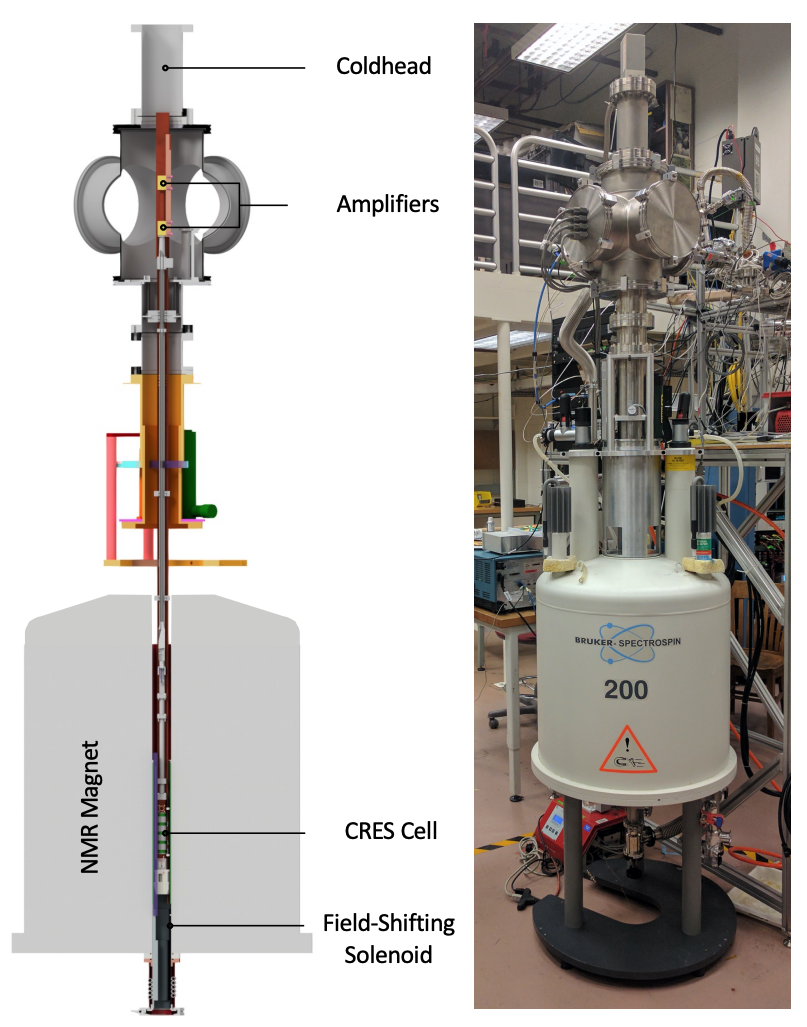
\includegraphics[width=0.55\textwidth]{figs/Chapter-3/phaseII_system.png}
    \caption{\label{fig:chap3-phase2-apparatus} The Phase II CRES apparatus used to perform the first measurement of the tritium beta-decay spectrum using CRES.}
\end{figure}

\subsubsection*{Magnet and Cryogenics}

The magnetic field for the Phase II experiment is provided by a nuclear magnetic resonance (NMR) spectroscopy magnet with a central bore diameter of 52~mm (see Figure \ref{fig:chap3-phase2-apparatus}). The magnet produces a background magnetic field with an average value of 0.959~T with a 10~ppm variation across the bore diameter achieved using several shim coils built into the magnet. Using an external NMR field probe, the variation of the magnetic field along the vertical axis of the magnet bore was measured to obtain an accurate model of the magnetic field so that the CRES cell could be positioned for optimal magnetic field uniformity.

An external solenoid magnet was installed inside the magnet bore to provide the ability to shift the magnitude of the background magnetic field by a few mT. The solenoid has inside diameter of 46~mm and a length of 350~mm, which terminates in a vacuum flange that allows it to be inserted into the NMR magnet bore from the bottom. By shifting the value of the magnetic field by a few mT, the cyclotron frequencies of electrons produced by the 17.8~keV $^{83m}$Kr internal-conversion line \cite{krypton83m} can be shifted by frequencies of $\pm100$~MHz. This allows one to study the frequency dependent behavior of several CRES systematics, such as detection efficiency, that directly affect the measured shape of the tritium spectrum. 

The inside of the magnet bore diameter was pumped down to a vacuum of less than 10~$\mu$torr using a turbomolecular pump, which allows for cryogenic cooling of the CRES cell and RF system. Cooling power was supplied to the Phase II apparatus using a cryopump with its coldhead mounted above the primary magnet and CRES cell. This arrangement allowed for sufficient cooling power to be delivered to the amplifiers to cool them to a temperature of $\approx 40$~K, while keeping the amplifiers far enough from the magnet so as not to be damaged by the large field strength. Thermal contact between the coldhead, amplifiers, RF system, and CRES cell is achieved using a copper bar that runs the full length of the apparatus. To prevent freeze-out of $^{83m}$Kr on the walls of the CRES cell a separate heater was installed to keep the CRES cell near a temperature of 85~K during the operation of the experiment.

\subsubsection*{CRES Cell}

Located in the most uniform region of the magnetic field is the CRES cell, which is the region of the apparatus where radioactive decays of $^{83m}$Kr and $T_2$ produce electrons that can be trapped and measured using CRES (see Figure \ref{fig:chap3-cres-cell}).
\begin{figure}[htbp]
    \centering
    \includegraphics*[width=0.65\textwidth]{figs/Chapter-3/apparatus.pdf}
    \caption{\label{fig:chap3-cres-cell} Diagram of the CRES cell portion of the Phase II apparatus.}
\end{figure}
The CRES cell is manufactured from a segment of cylindrical waveguide designed to operate at K-band frequencies near 26~GHz. The diameter of the waveguide determines which resonant modes of the waveguide will couple to the electron and transmit its radiation to the amplifiers. For Phase II a waveguide diameter of 1~cm was selected, which allows electrons to couple to the $\mathrm{TE}_{11}$ and $\mathrm{TM}_{01}$ cylindrical waveguide modes. To reduce complexity in modeling and analyzing the CRES data, it is ideal to select a diameter that prevents electrons from coupling to higher-order waveguide modes beyond the fundamental TE and TM modes. 

Around the exterior of the cylindrical waveguide are several magnetic coils used to produce magnetic traps inside the CRES cell volume. Without a magnetic trap electrons produced from decays inside the CRES cell quickly impact the cell wall, which prevents a measurement of their cyclotron frequency using CRES. Each coil along the length of the waveguide produces a separate trap that is approximately harmonic. By independently controlling the currents provided to each coil, the traps can be configured to have equal values of the magnetic field at the trap bottom despite a non-uniform field from the NMR magnet. 

Two primary magnetic trap configurations were used during the Phase II experiment. The first was a shallow trap configuration used primarily for its high energy resolution to study systematics using $^{83m}$Kr decays, and the second was a deeper trap that could trap a higher percentage of pitch angles. The trade-off with the deeper trap is that the higher trapping efficiency comes at the cost of lower energy resolution due to the greater variation in pitch angle (see Section \ref{sec:chap3-cres}). The deep trap was the trap used to measure the tritium beta-decay spectrum in Phase II.

The source gases were delivered into the CRES cell through a gas port located near the top end of the cylindrical waveguide. To prevent the gases from escaping the cell, vacuum tight RF transparent windows are needed to contain the tritium and krypton source gas across a 1~atm pressure differential, while still transmitting the cyclotron radiation without distortion. The crystalline material, $\mathrm{CaF}_2$, which has a thermal expansion coefficient similar to that of copper, was used for this purpose in the CRES cell. Two windows, each 2.4~mm thick, were used to seal off the ends of the CRES cell. The thickness of 2.4~mm corresponds to half of a cyclotron wavelength when one accounts for the permittivity of $\mathrm{CaF}_2$.

\subsubsection*{RF System}

The RF system in the Phase II apparatus propagates the cyclotron radiation from the CRES cell to the receiver chain. The receiver chain performs the down-conversion and digitization required to obtain signals that can be analyzed to determine the cyclotron frequencies of electrons in the CRES cell (see Figure \ref{fig:chap3-phase2-rf-chain}).
\begin{figure}[htbp]
    \centering
    \includegraphics*[width=0.95\textwidth]{figs/Chapter-3/230620_phase2_rf_chain.png}
    \caption{\label{fig:chap3-phase2-rf-chain} RF system diagram for the Phase II apparatus.}
\end{figure}

Below the CRES cell, at the bottom of the Phase II apparatus, is a tickler port and waveguide terminator. The tickler port is used to inject signals into the CRES cell and RF system for testing and calibration purposes. The waveguide terminator is designed to absorb cyclotron radiation emitted by electrons that transmits out of the bottom of the CRES cell. This lowers the total power received from electrons in the CRES cell, since all the energy radiated downwards is absorbed into the terminator. Earlier iterations of the Phase II apparatus used an RF short in this location that reflected this power up towards the amplifiers; however, interference between the upward traveling and reflected radiation led to a disappearance in the signal carrier that made reconstruction impossible.

Radiation traveling upward passes through the $\mathrm{CaF}_2$ window passes and a $\lambda/4$ plate, which transforms the circularly polarized cyclotron radiation into linear polarization. The linearly polarized fields next travel through a segment of circular waveguide that transitions into a long segment of WR-42 waveguide that carries the fields out of the high magnetic field region. A thermal break segment is included, which consists of a segment of gold-plated stainless steel WR-42 waveguide, to help thermally isolate the relatively warm CRES cell from the colder amplifiers. The radiation then passes through a cryogenic circulator, which prevents signals reflected from the amplifiers from interfering with the CRES cell before a WR-42 to WR-28 transition connects the waveguide to the first of the cyrogenic amplifiers. The radiation passes through two cyrogenic amplifiers before being coupled to a coaxial termination at the top of the Phase II apparatus.

The coaxial cable transfers the cyclotron radiation signals to a high-frequency mixing stage that performs an analog frequency down-conversion using a 24.5~GHz LO. Two forms of digitization can be used at this stage to read out the CRES data. One is a real-time spectrum analyzer that digitizes the CRES signal data in time-domain and computes the frequency spectrum in real-time, which allows for direct visualization of CRES signal spectrograms as the experiment is running. The real-time spectrum analyzer is most useful for taking small amount of streamed data for debugging and analysis of the system. The other method, which was used to collect the majority of the CRES data in Phase II, is a ROACH-2 FPGA and digitizer system. The ROACH system consists of a fast ADC that samples the CRES signal data at 3.2~GSps. Internal digital down-conversion stages implemented in the FPGA perform a mixing operation that reduces the bandwidth of the CRES signals to 100~MHz. The FPGA implements a 4096 sample FFT and packetizes time and frequency domain records in parallel. The packetized data is then transferred from the ROACH to be analyzed by the data-processing pipeline.

\subsection{CRES Track and Event Reconstruction}

\subsubsection*{Time-Frequency Spectrogram}

The online data-processing software uses a real-time triggering algorithm that identifies interesting data that could contain CRES signals. Triggered data are collected into files that are transferred to a server for offline processing and analysis. The data files contain a continuous series of time-domain samples, broken into a set of records, which are 4096 samples long. The time-series is made up of 8-bit IQ samples acquired at 100~MHz. 

Each time-series record is accompanied by an associated frequency spectrum consisting of 4096 frequency bins approximately 24.4~kHz wide, which is represented as a power spectral density. The individual frequency spectra can be organized temporally to create a time-frequency spectrogram that represents the evolution of the cyclotron frequency spectrum over the course of the CRES event (see Figure \ref{fig:chap3-tritium-event0-spectrogram}). 
\begin{figure}[htbp]
    \centering
    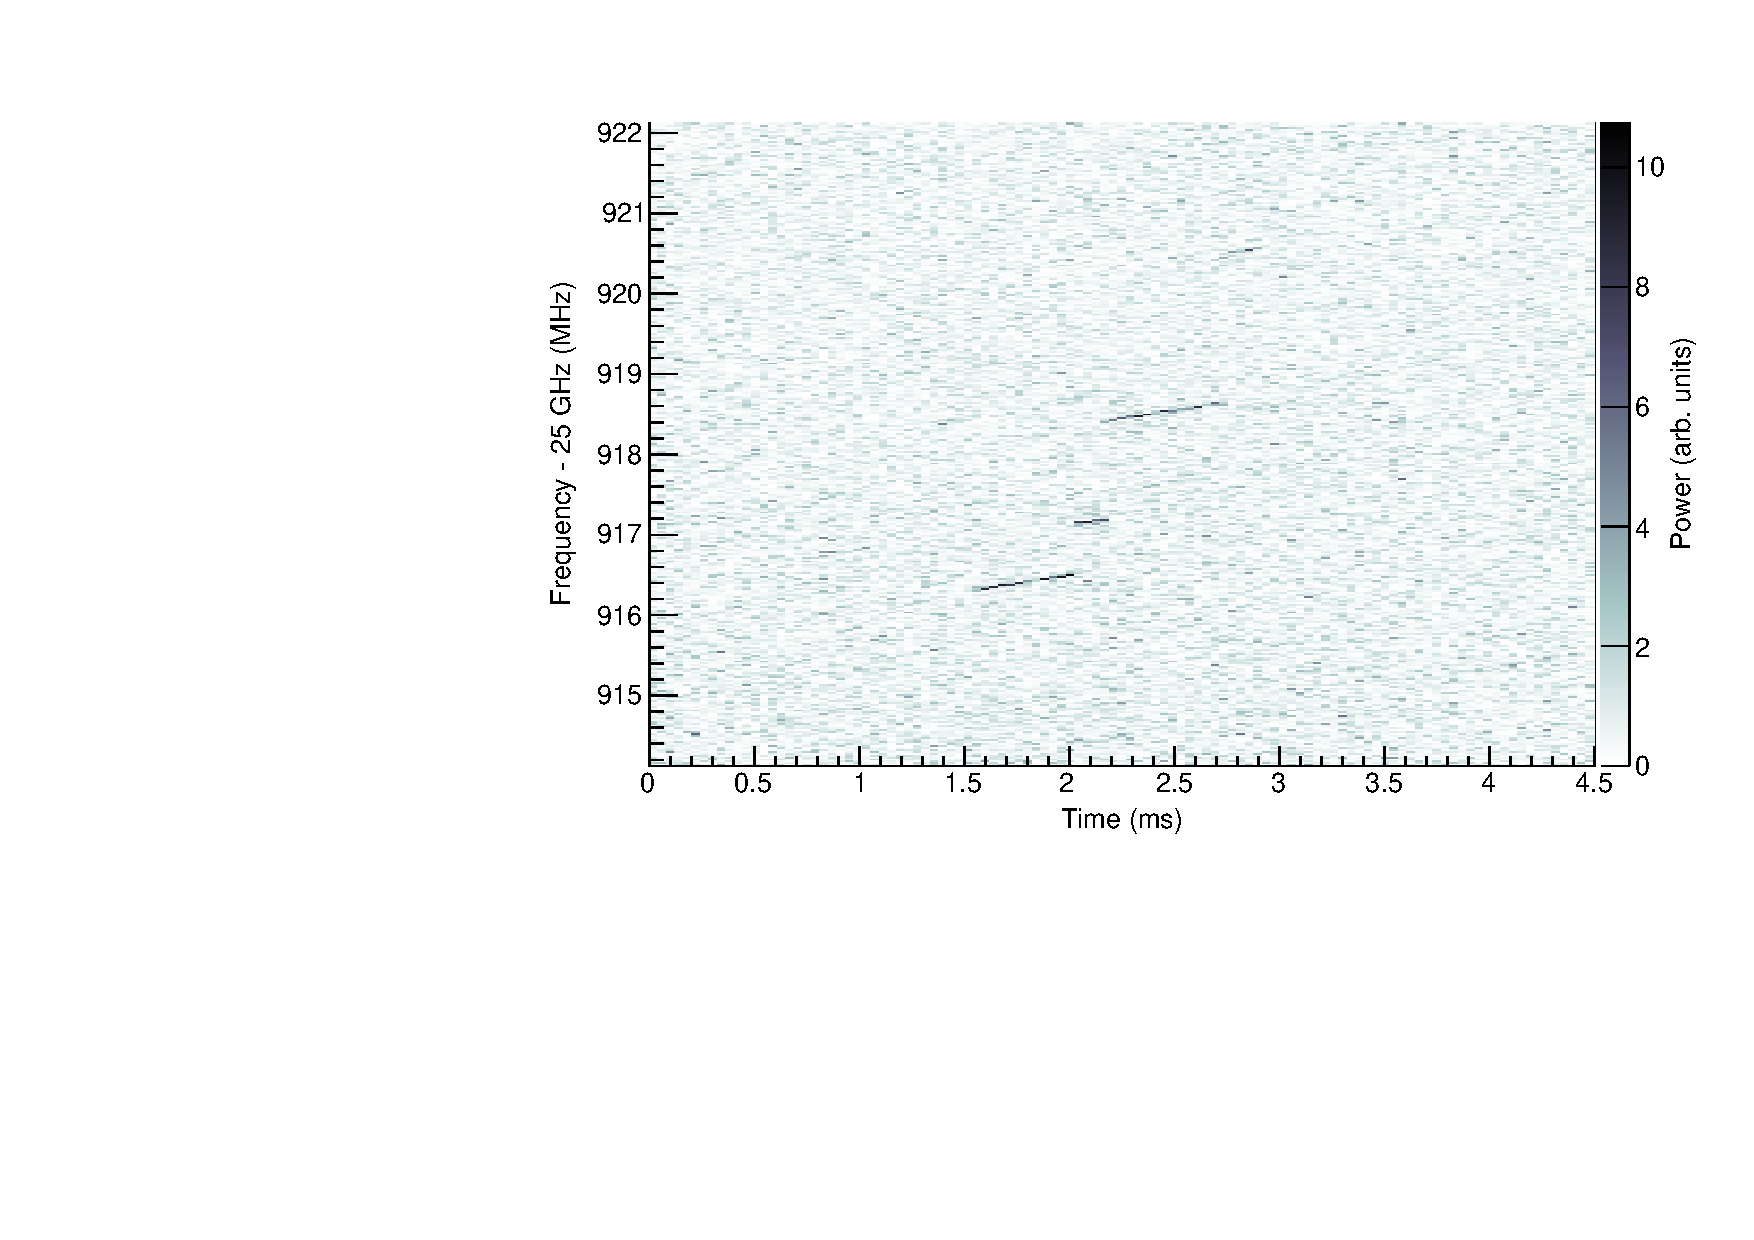
\includegraphics[width=0.7\textwidth]{figs/Chapter-3/T2_Event0.pdf}
    \caption{The time-frequency spectrogram of a tritium CRES event in the Phase II apparatus.}
    \label{fig:chap3-tritium-event0-spectrogram}
\end{figure}
The time-frequency spectrogram is represented as a two-dimensional image where the color of each pixel is proportional to the power spectral density. Each vertical slice of pixels in the image represents a frequency spectrum; therefore, each horizontal bin represents the data obtained over a duration of $4096\times 0.01$ $\mathrm{MHz}^{-1}=40.96$ $\mu$sec. 

\subsubsection*{CRES Event Data Features}

Phenomenologically, a CRES signal appears as a sinusoidal signal whose frequency slowly increases over time in what is called a frequency "chirp". Axial motion of the electron in the trap leads to the formation of frequency sidebands that surround the more powerful carrier frequency. The critical piece of information that must be extracted from the track and event reconstruction procedure is the carrier frequency, since it is this frequency that gives the cyclotron frequency and thus the kinetic energy. Axial motion from non-$90^\circ$ pitch angles changes the average magnetic field experienced by an electron, because the electron effectively samples the magnetic field along its trajectory. The change in the average magnetic field with pitch angle leads to different cyclotron frequencies that correspond to the same kinetic energy. However, because of the low-SNR in Phase II, sidebands were unable to be observed, so no attempt to correct for this effect was attempted. The effect of different pitch angles is to broaden the peak of a monoenergetic electron line, which can be quantified by measuring the instrumental resolution of the Phase II apparatus.

In the time-frequency spectrogram representation, the chriping carrier frequency appears as a linear track of high-power frequency bins (see Figure \ref{fig:chap3-tritium-event0-spectrogram}). The vertical slope of the tracks is caused by the emission of energy from the electron in the form of cyclotron radiation; therefore, the size of the slope parameter is directly proportional to the Larmour power. The continuous track is periodically interrupted by random jumps to higher frequency (lower energy) caused by random inelastic collisions with background gas molecules. The length of a track is an exponentially distributed variable whose mean value is inversely proportional to the gas density. The size of the frequency discontinuities is directly proportional to the energies of the rotational and vibrational states of background gas molecules. 

A CRES event refers to the collection of tracks produced by a trapped electron until it inevitably scatters into a pitch angle that can no longer be trapped. The goal of track and event reconstruction is to identify the set of tracks in a time-frequency spectrogram that represents a segment of data acquired in the Phase II apparatus. These tracks must be clustered into events, from which one can determine the first track produced by the electron and thus estimate its starting cyclotron frequency and kinetic energy. 

\subsubsection*{Track Reconstruction}

The first step in CRES event reconstruction is the identification of tracks in the time-frequency spectrogram, which is essentially an image processing task. Track finding starts by normalizing the power spectral density based on the average noise power. Next a power threshold is applied to the normalized spectrogram where only bins that have a SNR ratio greater than five are selected to build tracks. In this case SNR is defined as the ratio between the normalized, unitless power of a bin divided by the average normalized power across the full frequency spectrum.

\begin{figure}[htbp]
    \centering
    \includegraphics*[width=0.7\textwidth]{figs/Chapter-3/230621_t_event_zero_sparse_spectrogram_zoom.pdf}
    \caption{\label{fig:chap3-sparse-spectrogram} The sparse spectrogram obtained by placing a power cut on the raw spectrogram shown in Figure \ref{fig:chap3-tritium-event0-spectrogram}.}
\end{figure}

The sparse spectrogram produced by this power cut consists only of a sparse collection of high-power frequency bins that could be part of a CRES signal track (see Figure \ref{fig:chap3-sparse-spectrogram}). In this form is it much easier to identify tracks "by eye"; however, for the Phase II analysis Project 8 developed its own custom-made track finding algorithm, called the sequential track finder (STF). 

The STF algorithm processes the sparse spectrogram in sequential fashion, processing each time-slice one-by-one until the end of the spectrogram is reached. Tracks are found by searching for points in the sparse spectrogram that appear to fall on a straight line. Multiple configurable parameters are built into the STF algorithm that allow the user to tune the criteria for adding a point to an existing track or creating a new track. These include parameters such as maximum time and frequency differences between subsequent points in a track as well as minimum SNR values for the start and endpoints of the track. Additionally, tracks are required to have a minimum length and slope to be considered potential CRES tracks rather than random noise fluctuations. 

The resulting output of the STF is a collection of track objects that consist of the track point objects and their properties. The final step is to calculate track-level properties and apply cuts to reject false tracks found by the STF. This involves the fitting of a line to the collection of track points as well as the total and average power of the track obtained by computing the sum and mean of the points powers. The starting frequency of the track is determined by calculating the time coordinate that  intersects with the linear fit. A cut is then performed to remove all tracks that do not have a specified average power over their duration, which helps to remove the majority of noise fluctuations that have passed all previous cuts up to this point.

\subsubsection*{Event Reconstruction}

After track reconstruction comes event reconstruction, where the identified tracks are grouped into events that correspond to the trajectory of a single electron in the trap. This procedure attempts to match tracks head to tail by checking if the start and end times of a pair of tracks falls withing a certain tolerance. This tolerance is a configurable parameter that can be tuned to an optimal value using Monte Carlo simulations of events in the Phase II apparatus.

After the event building procedure has completed, there remains a small likelihood that false tracks have made it through to the event reconstruction stage. Typically, cuts at the track level are able to remove 95\% of the false tracks identified by the STF, which leads to a significant number of false tracks at the event building stage. However, the additional event-level information makes it possible to reject events that contain these false tracks with a high degree of confidence. 

Two event level features are associated with events caused by real electrons --- the duration of the first track as well as the number of tracks in the event. Real electrons tend to have event structures with longer first tracks and a higher number of total tracks. Based on the values of these two criteria, a minimum threshold on the average power in the first track was configured to reject false events. The average power in the first track was chosen due to the critical nature of the starting frequency of the first track in an event to the krypton and tritium spectrum analyses.

\subsection{Results from Phase II}

The main result from Phase II was the measurement of the tritium beta-decay spectrum using CRES, which lead to the first neutrino mass limit with CRES. However, Phase II also included a significant $^{83m}\rm{Kr}$ measurement campaign to understand important systematics relevant to the tritium spectrum measurement and the fundamentals of the CRES technique itself. This required high-resolution measurements of the $^{83m}\rm{Kr}$ internal-conversion spectrum \cite{krypton83m}, which is an interesting science result in its own right.

The results from Phase II represents a significant effort from entire Project 8 over several years. Because the focus of my contributions to Project 8 is directed towards the research and development efforts for the Phase III experiments, the goal in this section is not to provide a detailed description of the analyses that lead to the Phase II results. Rather, I will provide brief descriptions of a few plots representative of the main results from Phase II as reported in \cite{p8prl2023,p8prc2023}.

\subsubsection*{Measurements with Krypton}

Measurements with krypton were a key calibration tool for Phase II of the experiment and will continue to be useful in Phase III. Krypton measurements are CRES measurements of the internal-conversion spectrum of the metastable state of krypton-83, $^{83m}\rm{Kr}$, produced by electron capture decays of $^{83}\rm{Rb}$. A supply of $^{83}\rm{Rb}$ was built into the Phase II apparatus gas system that supplied the CRES cell with $^{83m}\rm{Kr}$ via emanation.

The $^{83m}\rm{Kr}$ internal-conversion spectrum consists of several lines based on the orbital of the electron ejected during the decay. The conversion lines useful to Project 8 are those that emit electrons with kinetic energies that fall inside the detectable frequency bandwidth of the Phase II apparatus. These are the K; L2 and L3; M2 and M3; and N2 and N3 lines; with kinetic energies of 17.8~keV, $\approx 30.4$~keV, $\approx 31.9$~keV, and $\approx 32.1$~keV, respectively. The different energies of the lines allows one to test the linearity of the relationship between kinetic energy and frequency across the range of frequencies covered by the continuous tritium spectrum.

\begin{figure}[htbp]
    \centering
    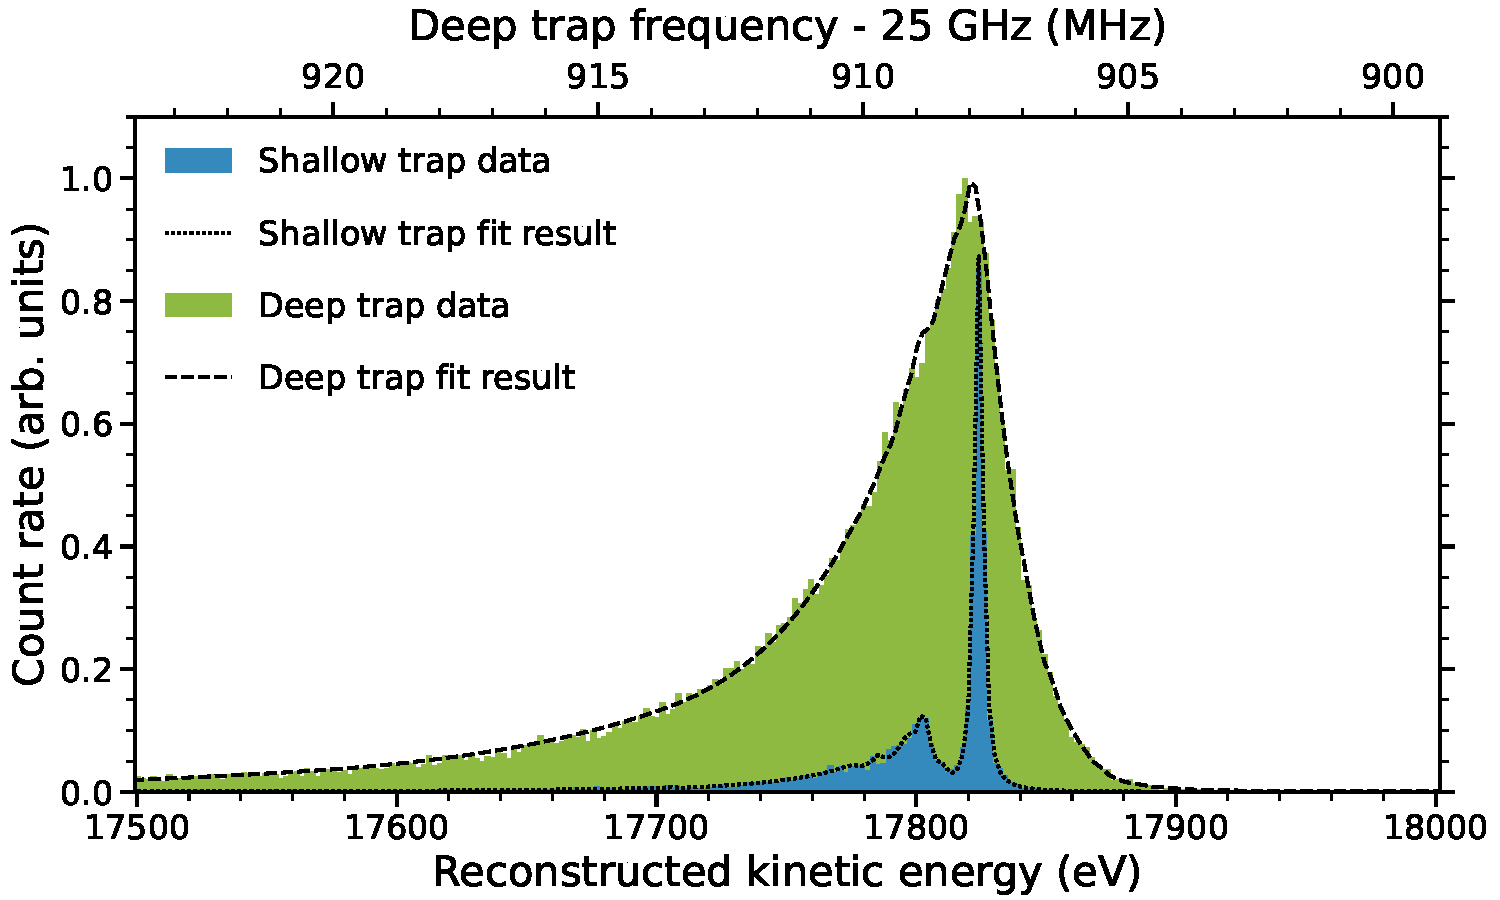
\includegraphics[width=0.7\textwidth]{figs/Chapter-3/kr_fit.pdf}
    \caption{Fits to the measured 17.8-keV $^{83m}\rm{Kr}$ conversion line using the deep and shallow trap configurations. }
    \label{fig:chap3-krypton-spec-fit}
\end{figure}

Numerous detector-related effects relevant to the tritium analysis can be characterized by measuring the shape of the krypton spectrum. Specific examples include variations in the magnetic field as a function of the radial position of the electron, variation in the magnetic field caused by the trap shape, variation in the average magnetic field for electrons with different pitch angles, and the effect of missing tracks due to scattering. These spectrum shape measurements focused on the 17.8-keV krypton line and utilized different trap geometries based on the particular goal of the dataset (see Figure \ref{fig:chap3-krypton-spec-fit}).

Krypton measurements with a shallow trap allow for high energy resolution, since variation in frequency due to pitch angle differences is sharply reduced in the shallow trap configuration. With this trap the main 17.8-keV peak of the conversion spectrum is clearly visible along with additional satellite peaks at lower energy, which correspond to the shakeup/shakeoff spectrum of the decay. The high accuracy of the fit demonstrates a high degree of understanding of the CRES systematics.

\begin{figure}[htbp]
    \centering
    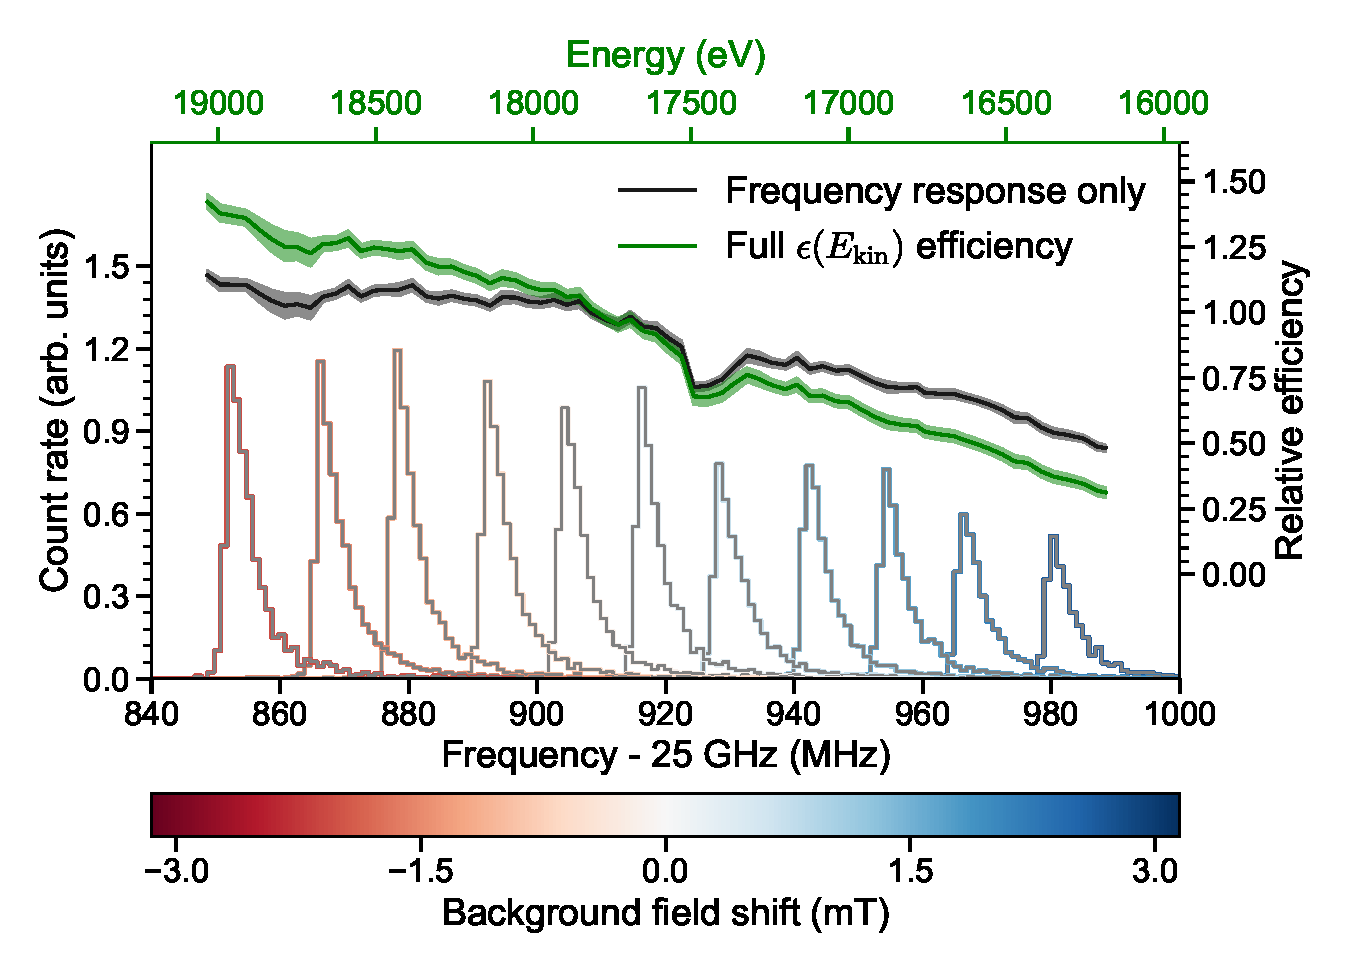
\includegraphics[width=0.7\textwidth]{figs/Chapter-3/fss_for_prl_plot.pdf}
    \caption{Measurements of the 17.8-keV $^{83m}\rm{Kr}$ line using the deep trap configuration for different values of the magnetic field from the field shifting solenoid.}
    \label{fig:chap3-fss-plot}
\end{figure}

The broadening of the krypton spectrum seen for the deeper track is due to the large range of electron pitch angles that can be trapped. Furthermore, with a deeper trap there is a larger parameter space of electron that could be produced with pitch angles that are trappable but not visible in the time-frequency spectrogram. These electrons remain in the trap and can scatter multiple times before randomly scattering to a visible pitch angle. This leads to one or more missing tracks earlier in the event, which leads to a misreconstruction of the true starting frequency. By measuring the krypton spectrum shape in the same trap used to detect tritium events, the effect this has on the spectrum shape can be characterized to mitigate its impact on the tritium measurements.

Changes in the Krypton spectrum shape as a function of CRES frequency were used to study the detection efficiency of the Phase II apparatus. Variations in the detection efficiency as a function of frequency directly influences the measured shape of the continuous tritium spectrum, which can lead to errors in the neutrino mass estimate if not modeled appropriately. Using the field-shifting solenoid (FSS) the cyclotron frequency of the krypton 17.83~keV line was shifted across the full frequency range of the tritium spectrum data (see Figure \ref{fig:chap3-fss-plot}). The FSS is a wound copper solenoid magnet that surrounds the CRES cell. Controlling the current through this magnet allows one change the value of the background magnetic field and the frequency of the krypton conversion lines. Variations in the deep trap krypton spectrum shape can be used to infer the detection efficiency as a function of frequency and correct for this affect in the tritium measurements.

\subsubsection*{Tritium Spectrum and Neutrino Mass Results}

The tritium measurement campaign resulted in the collection of 82 days of detector live time during which 3770 total tritium events were detected. The track and event reconstruction analysis extracted the starting frequencies of these tritium events, which were used to build a frequency spectrum of tritium beta-decays. The resulting frequency spectrum was then converted to an energy spectrum using the information gleaned from the krypton measurement campaign to obtain the tritium beta-decay spectrum (see Figure \ref{fig:chap3-final-tritium-fit}).
\begin{figure}
    \centering
    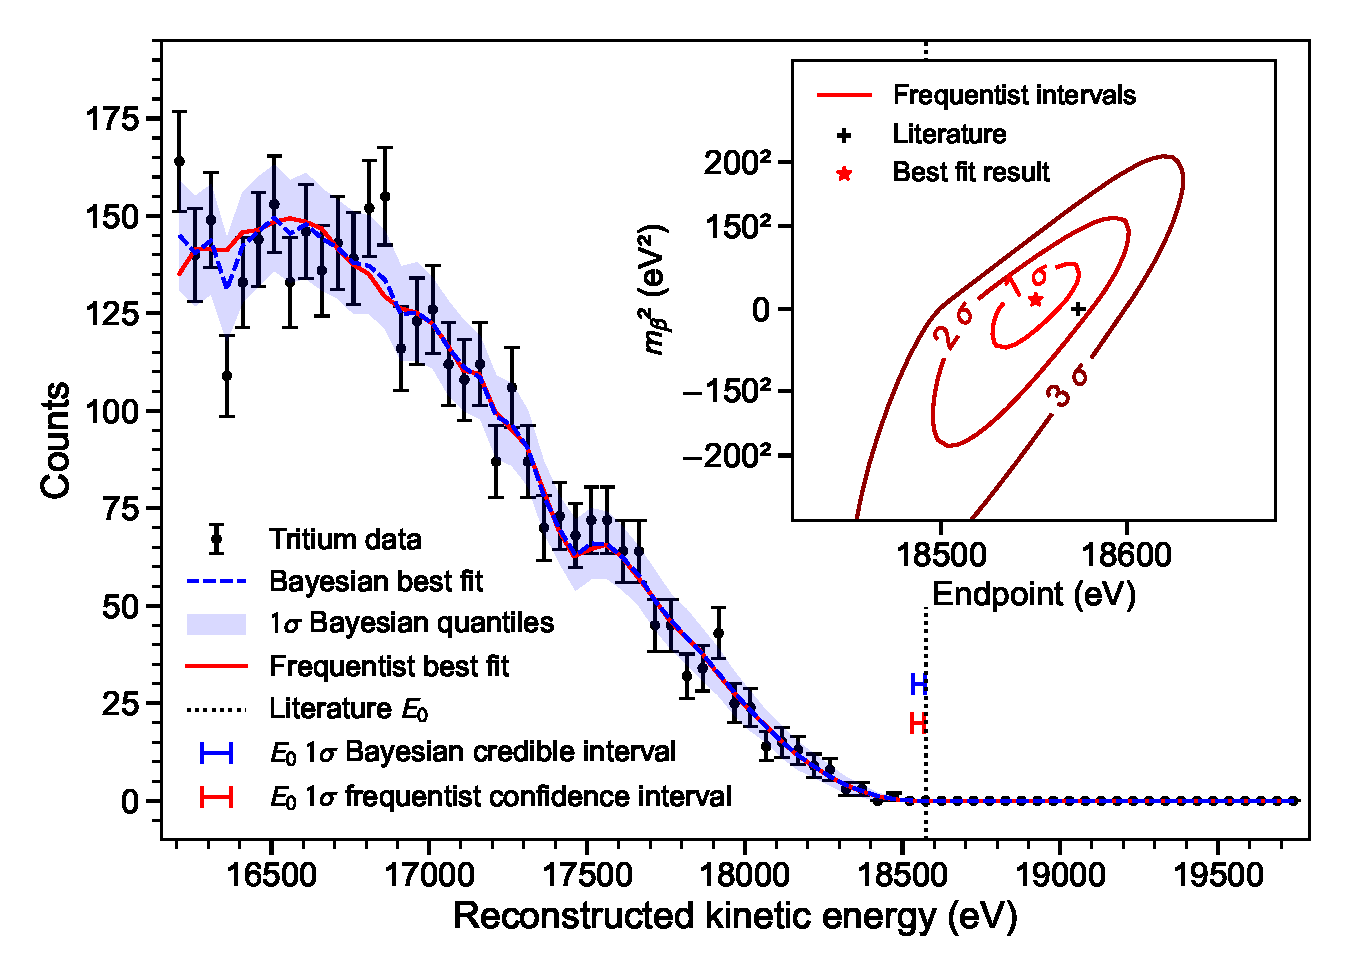
\includegraphics[width=0.7\textwidth]{figs/Chapter-3/12-03-22A_final_E0_real_data_phase_II_tritium_fit_1d.pdf}
    \caption{The measured tritium spectrum from Phase II with Bayesian and frequentist fits.}
    \label{fig:chap3-final-tritium-fit}
\end{figure}

CRES is inherently a very low background technique with the dominant source of noise being random RF fluctuations. Monte Carlo simulations, validated using measurements of the RF noise background, were used to set track and event cuts to guarantee that zero false events would occur over the duration of the experiment with 90\% confidence. Notably, the measured spectrum has zero events beyond the tritium spectrum endpoint, which allows one to constrain the background rate in the Phase II apparatus to less than $3\times10^{-10}$~counts/ev/s. Achieving a low background is critical for future neutrino mass experiments that seek to measure the neutrino mass with less than 100~meV sensitivity.

Bayesian and frequentist based fits to the measured tritium spectrum, incorporating information gained about CRES systematics from the krypton measurements, were performed to extract upper limits on the tritium beta-decay spectrum endpoint as well as the neutrino mass. The estimated spectrum endpoints are $18553^{+18}_{-19}$~eV for the Bayesian analysis and $18548^{+19}_{-19}$~eV for the frequentist analysis. The quoted uncertainties are 1-$\sigma$, and both results are within 2-$\sigma$ of the literature endpoint value of 18574~eV. The estimated neutrino mass for both results is consistent with $m_\beta^2=0$. The 90\% confidence upper limits for the Bayesian analysis is $m_\beta < 155$~$\rm{eV}/\rm{c}^2$ and $m_\beta < 152$~$\rm{eV}/\rm{c}$ for the frequentist analysis.

Though the neutrino mass results from Phase II are not competitive with KATRIN, the experiment was a promising first step towards the development of more precise neutrino mass measurements using CRES. The low-background and high-resolution achievable with krypton measurements are promising features of the technique that were demonstrated with the Phase II apparatus. As new technologies are developed to enable CRES measurements in larger volume, many of the lessons learned from Phase II will continue to influence the operation and design of future experiments.

\section{Phase III R\&D: Antenna Array CRES}
\label{sec:chap3-phaseIII-antenna-arrays}

The goal of Phase III in the Project 8 experimental program is to develop the technologies and expertise required to build an experiment that uses CRES to measure the neutrino mass with a target sensitivity of 40~meV. One of the key technologies is a method for performing high resolution CRES measurements in a large volume, which allows one to observe a sufficient quantity of tritium to measure the low-activity endpoint region of the tritium spectrum. 

\subsection{The Basic Approach}

One possible approach, suggested in the original CRES publication \cite{p8originalcres}, is to use many antennas to surround a volume of tritium gas in a magnetic field (see Figure \ref{fig:chap3-antenna-concept-cartoon}). When a decay occurs the electron will emit cyclotron radiation that can be collected by the array and used to perform CRES.
\begin{figure}[htbp]
    \centering
    \includegraphics*[width=0.6\textwidth]{figs/Chapter-3/230614_antenna_cartoon.png}
    \caption{\label{fig:chap3-antenna-concept-cartoon} A cartoon illustration of the basics of the antenna array CRES technique.}
\end{figure}
Each antenna in the array collects only a small fraction of the electron's signal power, which is less than 1~fW for a 18.6~keV kinetic energy electron in a 1~T magnetic field. Scaling to large volumes with the antenna array approach is accomplished by increasing the number of antennas in the array, which increases the volume available for CRES measurements. 

Several features of the antenna array approach make it an attractive candidate technology for a large volume experiment. One example is the accurate position reconstruction possible with a multichannel antenna array. Using techniques like digital beamforming, it is possible to estimate the radial and azimuthal positions of the electron in the magnetic trap with a precision significantly less than the size of the cyclotron wavelength. This capability allows one to perform event-by-event estimations of the magnetic fields experienced by an electron, which helps achieve high energy resolution with the CRES technique.

The easy availability of position information with the antennas array approach is potentially a unique advantage that provides significant flexibility in the magnetic field uniformity requirements compared to other proposed approaches to large volume CRES (see Chapter \ref{chap:cavity}). Spatial discrimination using digital beamforming leads to pileup reduction, which helps to reduce the potential of background events caused by missing tracks or by incorrectly clustering a group of tracks into an event. Limits on the background rate for a neutrino mass measurement with 40~meV sensitivity are stringent and the total activity of the tritium source is gigantic relative to the activity near the endpoint. Thus, pileup discrimination could be an important tool for a large scale CRES experiment.

Another beneficial quality of antenna arrays is that the volume of the experiment can be scaled independent of frequency by simply adding more antennas to the array (see Figure \ref{fig:chap3-phaseiv-antenna}). Resonant cavities, the proposed alternative large volume CRES technology, are ideally operated in magnetic fields that cause electrons to move with cyclotron frequencies near the fundamental cavity resonance, to avoid complex coupling of the electron to multiple cavity modes simultaneously. This leads to a coupling between the cavity volume and the magnetic field magnitude, which forces one to lower the magnetic field in order to increase the experiment scale. Whereas, for antenna arrays, in principle there is no physical limitation on the size of the antenna array that can be used at a particular magnetic field. However, this approach to scaling an antenna array experiment leads to rapidly increasing cost and complexity due to the large number of antennas, amplifiers, and data streams, which require substantial computer processing power to effectively utilize. The link between array size and computational cost will be explored in Section \ref{sec:chap4-pter}.

\subsection{The FSCD: Free-space CRES Demonstrator}
\label{sec:chap3-fscd}

The complexity of the antenna array CRES technique requires the construction of a small scale demonstration experiment to develop an understanding of technique itself and relevant systematics. Without a demonstrator experiment it is not possible to sufficiently retire the technical risks associated with the full-scale experiment. Therefore, Phase III of the Project 8 experimental program is primarily focused on the development and operation of demonstrator experiments to inform the design of the Phase IV experiment.

The Phase III demonstrator experiment for antenna array CRES is called the Free-space CRES Demonstrator or FSCD. The FSCD is also a capable neutrino mass measurement experiment in its own right, with a target neutrino mass sensitivity of a few eV using a molecular tritium source. The higher-costs associated with antenna-based CRES, which were identified over the course of the development of the FSCD, have lead to the adoption of resonant cavities as the technology of choice for Phase III.%Therefore, all future development of the FSCD and antenna-based CRES in Project 8 has been suspended. 

\subsubsection*{Magnetic Field}

The background magnetic field for the FSCD is provided by a hospital-grade MRI magnet (see Figure \ref{fig:chap3-mri-magnet}). The magnet produces a magnetic field of approximately 0.958~T, which corresponds to a tritium spectrum endpoint frequency of approximately 25.86~GHz. 
\begin{figure}[htbp]
    \centering
    \includegraphics*[width=0.5\textwidth]{figs/Chapter-3/230614_mri_magnet.png}
    \caption{\label{fig:chap3-mri-magnet} An image of the MRI magnet installed in the Project 8 laboratory at the University of Washington, Seattle.}
\end{figure}
The magnet is installed in the Project 8 laboratory located at the University of Washington, Seattle, and is shimmed to produce a uniform magnetic field with variations on the ppm-level. Measurements of the magnetic field non-uniformities are performed using a NMR probe and rotational gantry to capture measurements of the magnetic field around an elliptical surface in the center of the MRI magnet. During the operation of the FSCD an array of Hall or NMR magnetometers would be used to periodically measure the magnetic field to monitor its time stability.

Inside the field of the MRI additional electromagnets would be installed that provide the capability to shift the value of the background magnetic field and produce a magnetic trap. Shifting the background magnetic field by a few $\mu$T lets one control the cyclotron frequencies of electrons with a fixed kinetic energy, which is key to an effective calibration of the FSCD. The preferred calibration method for the FSCD is a mono-energetic electron gun that can inject electrons into the magnetic trap with a known kinetic energy. In combination with the field shifting magnet, one can vary the cyclotron frequencies of the electrons to measure the response of the antenna array as a function of the radiation frequency and electron position. This procedure characterizes the response of the antenna array and provides further information on magnetic field uniformity, which important to achieving good energy resolution.

The design of the magnetic trap is absolutely critical to the success of a CRES experiment. The ideal shape is the perfect magnetic box, which has a flat bottom and step function walls. Any variation in the average magnetic field experienced by an electron leads to changes in the cyclotron frequency that can make determining the true starting kinetic energy more difficult. This includes changes in the magnetic field caused by the walls of the magnetic trap as well as radial magnetic field variations. 

The ideal box trap is completely uniform and has infinitely steep walls that cause no change in the electron's cyclotron frequency as it is reflected from the trap wall. However, such a trap cannot be made from any combination of magnetic coils since it violates Maxwell's equations. One of the goals of magnetic trap design is to identify the configuration of coils that produces a trap that approximates the perfect box trap as closely as possible.

\subsubsection*{Antenna Array}

The canonical antenna array design for CRES is a uniform cylindrical array of antennas that surrounds the magnetic trap volume. Since the FSCD is a demonstrator experiment, the simplest and lowest cost version of a uniform cylindrical array is used, which is a single circular ring of antennas. The FSCD array design has a diameter of 20~cm (see Figure \ref{fig:chap3-fscd-render}).
\begin{figure}[htbp]
    \centering
    \begin{subfigure}{0.5\textwidth}
        \includegraphics*[width=\textwidth]{figs/Chapter-3/230614_fscd_render.png}
        \caption{}
    \end{subfigure}
    \hfill
    \begin{subfigure}{0.4\textwidth}
        \includegraphics*[width=\textwidth]{figs/Chapter-3/230614_5slot_model.png}
        \caption{}
    \end{subfigure}
    \caption{\label{fig:chap3-fscd-render} (a) A model of the FSCD antenna array, magnetic trap, and tritium containment vessel design.(b) A more detailed model of a prototype design for the 5-slot waveguide antenna design.}
\end{figure}
Along this circle are sixty slotted waveguide antennas that fully populate the available space around the array circumference. It is optimal to cover as large a fraction of the solid angle around the magnetic trap as possible in order to maximize the power collected from each electron . 

The distance between antennas around the circumference of the array is proportional to the wavelength of the cyclotron radiation. Therefore, maximizing the solid angle coverage of the array, while minimizing channel count to keep the hardware and data acquisition costs manageable, biases one towards smaller array diameters. Antenna near-field effects limit the minimum diameter of the array for a given antenna design, since the radiation from electrons that are too close to the array cannot be detected due to destructive interference. 

Slotted waveguide antennas are used in the FSCD antenna array due to their high efficiency and low loss, which comes from the lack of dielectric materials in the antenna structure. Coupling to the waveguide is performed with a coaxial cable connected at the center of the antenna. One of the drawbacks of waveguide antennas is the large amount of space required to fit them inside the limited MRI magnet volume. Alternative antenna designs, constructed from microstrip printed circuit boards require significantly less space at the cost of slightly higher energy losses in the antenna structure. 

The FSCD antenna design is a 5~cm long segment of WR-34 waveguide with 5 vertical slots cut into the side. The distance between slots along the length of the waveguide is a half wavelength for optimal power combination between the individual antenna slots. Each slot is offset from the center of the antenna face a small distance in order to most effectively couple the slot to waveguide modes inside the antenna.

The passive power combination achieved by placing 5 slots in a single waveguide is a compromise intended to reduce the cost and complexity of the antenna array system. Each additional channel in the array requires its own cryogenic amplifier and also increase the required computer power to process the raw data collected by digitizing each channel. Passive summation, achieved by combining antennas into arrays axially, reduces the array channel count at the cost of losses from imperfect passive combination.

Interference and re-radiation eventually limit the axial extent of passive power combination. The 5-slot designed developed for the FSCD is optimized to minimize the impact of these losses while achieving the maximum amount of axial coverage with a single ring of antennas. Scaling beyond the volume covered by a single ring of antennas is achieved by stacking additional rings of antennas together to cover a larger trap volume. A likely scenario for the FSCD experiment involves a staged experiment approach, where first a series of measurements is performed using only a single ring of antennas followed by experiments that add additional rings to the FSCD. The goal would be to first understand the principles of antenna array CRES using the simplest possible experiment, before attempting to scale the technique by expanding the antenna array size. 

\subsubsection*{Tritium Source}

While the primary purpose of the FSCD is as a technology demonstrator, it is impossible to retire all risks relevant to the Phase IV experiment without an intermediate scale measurement of the neutrino mass. Therefore, the FSCD has the scientific goal of measuring the neutrino mass with a rough sensitivity goal in the range of a few eV. This level of precision is achievable using a molecular tritium source with a volume of approximately 1~L at a density comparable to potential Phase IV scenarios.

Unlike previous CRES experiments, where the tritium source could be colocated with the receiving antenna inside a waveguide transmission line, the tritium source in the FSCD is thermally isolated from the antenna array to avoid freeze-out of the tritium molecules. The tiny radiation power emitted by electrons requires a system noise temperature of $\approx 10$~K or less, in order to detect events at a high enough efficiency to reach the neutrino mass sensitivity goals of the experiment. Achieving a system noise of 10~K requires that the antenna array and amplifiers operate at liquid helium temperatures of $\approx 4$~K, which significantly lowers the vapor pressure of molecular tritium. By keeping the molecular tritium isolated in an RF-transparent vessel the tritium gas can be kept at a relatively warmer temperature in the range of 30~K to avoid the accumulation of tritium on the experiment surfaces. 

\subsubsection*{Data Acquisition and Reconstruction}

A fundamental change in the data acquisition system for the FSCD is the shift from single to multichannel reconstruction. This transition results in a significant increase in the data-generation rate, which is linearly related to the number of independent channels in the array. The larger data volume coincides with an increased demand for computer processing power based on the need for more precise signal reconstruction algorithms driven by the FSCD and Phase IV sensitivity goals. Therefore, the data acquisition system for the FSCD is likely to represent a significantly larger fraction of the experiment cost and complexity than in Phase II.

Each antenna is connected to a cryogenic amplifier and down-converted from the 26~GHz CRES frequency using an IQ-mixer to reduce the size of the analysis window. Using an LO with a frequency of approximately 25.80~GHz the antenna array signals can be digitized at a rate of 200~MHz, which is sufficient bandwidth to resolve the complete sideband spectrum produced by axial oscillations of electrons in the FSCD magnetic trap. 

Direct storage of the raw FSCD antenna array data is undesirable, since the estimated amount of raw data generated is $O(1)$~exabyte per year. The storage of such a large dataset is infeasible for a demonstrator experiment like the FSCD, since it would represent a disproportionate fraction of the total experiment budget in Phase III and Phase IV. Therefore, a goal of the FSCD experiment is the development of real-time reconstruction methods that could reduce the raw data volume by detecting and reconstructing CRES events in real-time. Ultimately, a real-time CRES reconstruction pipeline is desired, which takes raw voltages samples from the antenna array and converts them into measured starting kinetic energy values for electrons.

The feasibility of a real-time reconstruction pipeline rests on the development of computationally efficient algorithms that can be implemented without the need for enormous computing resources. One challenge with the antenna array approach is that the small radiation power of a single electron is distributed among all channels in the array, such that reconstruction using only the information in a single channel is not possible. Therefore, simply performing the initial step in reconstruction --- signal detection --- requires orders of magnitude more computational power than previous CRES experiments. This operation will then be followed by other, potentially more expensive, reconstruction steps that are required in order to determine the kinetic energy of the electron.

\section{Pilot-scale Experiments}
\label{sec:chap3-freq-choice-and-pilot-scale}

The Project 8 pilot-scale experiment represents the experiment that retires all technical and engineering risks with Project 8's neutrino mass measurement approach, by combining all the required components of Phase IV in a multi-cubic-meter experiment. The larger scope and complexity of the pilot-scale experiment requires a careful choice of magnetic field and cyclotron frequency since this directly affects the design of nearly all parts of the experiment. Currently, designs for the pilot-scale experiment are in the conceptual stage, but a goal of Phase III is to translate these design concepts into detailed technical designs and specifications.

\subsection{Choice of Frequency}
The optimal CRES frequency for Project 8 is that which reaches the target sensitivity of 40~meV, while minimizing the cost and complexity of the overall experiment. The CRES frequency is directly linked to the magnetic field, which is coupled to nearly all aspects of the experiment design; therefore, an optimization of CRES frequency is effectively an optimization of the sensitivity of the overall experiment.

\subsubsection*{Frequency Scaling Laws}

The Phase I and II experiments utilized a background magnetic field of 0.959~T provided by an NMR magnet. Since this magnet was already available, the 0.959~T background field was selected for convenience. However, one additional reason to use this background field is that the cyclotron frequencies for electrons near the tritium endpoint in a 0.959~T field are approximately 26~GHz, which is within the standard RF Ka-band. Therefore, microwave electronics specialized for these frequencies are obtainable for relatively low cost. The operating frequency for the large-scale experiments must be selected in a more rigorous manner due to the increased scale and complexity of the systems as well as the requirements of the 40~meV neutrino mass science goal.

There is a bias towards lower frequencies in a large-volume experiment, due to the direct relationship between wavelength and the physical size of the compatible RF components like antennas and cavities. With a longer wavelength more volume can be surrounded by an array with fewer antennas, which reduces hardware and data-processing costs. Additionally, the size of a cavity experiment is directly proportional to the wavelength, since this sets the physical dimensions of the cavity. It is also simpler to engineer a magnet that provides a uniform magnetic field across several cubic-meters of space at lower magnetic fields, which provides advantages in terms of cost-reduction.

A concern with lower magnetic fields and frequencies is the power scaling as described by the Larmour equation, in which power is proportional to the square of the frequency. Naively, one would predict that the SNR would decrease with lower fields; however, two additional scaling laws that affect the noise power also come into play. Noise power is directly proportional to the required bandwidth, which decreases linearly with the magnetic field. Furthermore, at lower frequencies it is possible to purchase amplifiers with lower noise temperatures until approximately 300~MHz, at which point this relationship tends to flatten. Therefore, it is expected that the SNR remains approximately constant as the frequency decreases.

The fact that large-volume experiments are simpler to achieve at lower frequencies, and that SNR is expected to be approximately the same motivate the usage of lower magnetic fields in the large-scale experiments. This is simply because a low-frequency experiment is less costly than a high-frequency experiment and there is little to no penalty in SNR or detection efficiency at these fields.

One drawback of lower magnetic fields is the increased influence of external magnetic fields on the experiment. This includes magnetic fields from the building materials as well as variations in the earth's magnetic field. A suitable magnetic field correction system will need to be devised to deal with these effects, which includes constant monitoring of external fields.

\subsubsection*{Atomic Tritium Considerations}

The pilot-scale experiments will be the first Project 8 experiments to combine CRES with atomic tritium; therefore, the optimal frequency should take into account the affect of the background magnetic field on the atom trap.
\begin{figure}[htbp]
    \centering
    \begin{subfigure}{0.46\textwidth}
        \includegraphics*[width=\textwidth]{figs/Chapter-3/gloss.pdf}
        \caption{}
    \end{subfigure}
    \hfill
    \begin{subfigure}{0.49\textwidth}
        \includegraphics*[width=\textwidth]{figs/Chapter-3/dipolarloss.pdf}
        \caption{}
    \end{subfigure}
    \caption{(a) A plot of the decay rate for the two-body dipolar spin exchange interaction for cc and dd state. (b) A plot of the decay rate of the dipolar spin exchange interaction for d+d states as a function of magnetic field magnitude. Lowering the magnetic field is key for reducing the losses from this interaction.}
    \label{fig:chap3-dipolarloss}
 \end{figure}
 The primary influence of the background field magnitude is through the rate of dipolar spin-flips caused by a spin exchange interaction between trapped atoms \cite{tritium_spin_exchange}. 
 
 Atomic tritium is a simple quantum system with a hyperfine structure given by the addition of the nuclear and atomic spins. The addition of two spins leads to a hyperfine structure with four states in the $(m_s,m_I)$ basis \cite{tritium_hyperfine}. The states with atomic spins directed antiparallel to the magnetic field have $m_s=-1/2$ and are labeled as the a and b states. The a and b states are colloquially known as high-field seeking states, since their energy is minimized when in regions of higher magnetic field. This leads to losses in the magnetic trap as these atoms are drawn to higher fields away from the trap center. Alternatively, the c and d states, with atomic spin $m_s=+1/2$, minimize their energy in low magnetic fields because of the parallel alignment between spin and the magnetic field. Therefore, these low-field seeking states tend to stay trapped significantly longer than the high-field seeking states.

It would be advantageous to prepare tritium atoms in purely c and d states before trapping; however, even in this case losses still occur due to dipolar interactions between pairs of c and d states leading to flipped atomic spins and subsequent losses from high-field seeking atoms. The rate of these interactions depends on the magnitude of the background magnetic field and is maximal for dd interactions around 1~T (see Figure \ref{fig:chap3-dipolarloss}). The rate of losses from these interactions at 1~T requires atomic tritium production at a rate two orders of magnitude larger than at 0.1~T, thus, requirements on the whole atomic tritium system are significantly relaxed at lower magnetic fields, which provides powerful argument for moving to lower frequencies with the pilot-scale experiments and Phase IV.

\subsection{Pilot-scale Experiment Concepts}

\begin{figure}[htbp]
    \centering
    \includegraphics*[width=0.9\textwidth]{figs/Chapter-3/phaseiv_concept_sketch_ver2.png}
    \caption{\label{fig:chap3-phaseiv-antenna} A conceptual sketch of a large-volume antenna array based CRES experiment to measure the neutrino mass.}
\end{figure}

While the pilot-scale experiments are still in the early stages, enough is known to sketch the general features of these experiments at the conceptual level. Development of the antenna-based experiment has been suspended in favor of the cavity-based experiment.

\subsubsection*{Pilot-scale Antenna Array CRES Experiment Concept}

A conceptual design for an antenna-based CRES experiment is shown in Figure \ref{fig:chap3-phaseiv-antenna}. A large solenoid magnet provides a uniform background magnetic field less than 0.1~T in magnitude. Inside this region is the atom trapping magnet that generates a high magnetic field at the walls, which decays exponentially towards the central region. 
Known magnet designs that produce suitable atom trapping fields include Ioffe-Pritchard traps \cite{ioffe_trap}, which use conducting coils, as well as a Halbach array \cite{halbach_trap} made from permanent magnets. Either magnet choice produces a region of high magnetic fields, which excludes atoms and allows for the placement of antennas inside the experiment. 

Inside this region an array of microstrip patch antennas is inserted to collect the cyclotron radiation without providing a surface for atomic tritium recombination. Due to the lower frequency of cyclotron radiation antennas of a larger size can be used, which lowers the total number of antennas required to observe the experiment volume. Because of this scaling, the lower frequency experiment uses a similar number of antennas compared to a much smaller demonstrator experiment with a 1~T magnetic field.

The atomic tritium beamline that supplies fresh tritium atoms to the experiment is not shown in the figure. The general configuration matches the one shown for the pilot-scale cavity experiment (see Figure \ref{fig:chap3-cavity-pilot-scale}).

\subsubsection*{Pilot-scale Cavity CRES Experiment Concept}

The pilot-scale cavity experiment includes both an atomic tritium system and cavity CRES system. The atomic system consists of a thermal atom cracker located at the start of an evaporatively cooled atomic beamline. The atomic tritium system provides a supply of tritium atoms to the trap with temperatures on the order of a few mK. Atoms at this temperature can be trapped magneto-gravitationally, which is the reason for the vertical orientation of the cavity. At these low magnetic fields the trapping requirements for electrons and atoms differ enough such that it is advantageous to decouple the trapping potentials to avoid radioactive heating of the tritium atoms from excess trapped electrons. Electron trapping is provided by a set of magnetic pinch coils at the top and bottom of the cavity and a multipole Ioffe or Halbach magnet serves to contain the atoms.

\begin{figure}[htbp]
    \centering
    \includegraphics*[width=0.8\textwidth]{figs/Chapter-3/CavityAndBeamAndPerson2.pdf}
    \caption{\label{fig:chap3-cavity-pilot-scale} A conceptual sketch of a pilot-scale cavity CRES experiment with an atomic tritium beamline.}
\end{figure}

The cavity design for the pilot-scale experiment consists of a large cylindrical cavity with a TE011 resonance of 325~MHz. Such a cavity is truly enormous, with a diameter of approximately 1.2~m and a height of 11~m. When an electron is produced inside the cavity with a cyclotron frequency that matches the TE011 resonant frequency, its cyclotron orbit couples the electron to the TE011 mode, which drives a resonance in the cavity. These resonant fields can be read-out using an appropriate cavity coupling mechanism located at the center of the cavity. For more information on the cavity approach to CRES see Chapter \ref{chap:cavity}.

The bottom of the cavity has a cone termination to match the contour of the atom trapping magnet. This shape still allows for TE011 resonances with high internal Qs, which are required for good SNR in the cavity experiment. A small opening in the bottom of the cone serves as an entry point for the tritium atoms. To allow for calibration of the magnetic field inhomogeneities with an electron gun, the top of the cavity is left nearly completely open. Normally, this would drastically lower the Q-factor of the TE011 mode, but a specially configured coaxial partition is inserted at the top. This termination scheme is designed to act as a perfect short for the TE011 mode since the circular shape of the partition matches the electric field boundary conditions for the TE011 mode. Simulations with HFSS have confirmed that this design results in a high quality TE011 resonance despite the nearly completely open end.

\section{Phase IV}

The baseline CRES technology being pursued by Project 8 are resonant cavities, which, due to their geometric properties, simple CRES signal structure, and low channel count, appear to be the better option for Phase IV. The current knowledge of the antenna array CRES approach reveals no technical obstacles that would preclude it as a baseline technology for Phase IV, though it would certainly be significantly more expensive. Therefore, antenna arrays represent a fallback approach if resonant cavities prove infeasible.

The sensitivity of the pilot-scale atomic tritium experiment is estimated to be on the order of 0.1~eV, which means that increasing the sensitivity to reach the Phase IV goal will require an even larger experiment. Because of the direct coupling between the RF characteristics of a cavity and its geometry, the baseline plan is to build multiple copies of the pilot-scale experiment (see Figure \ref{fig:chap3-p4-render}) to obtain the required amount of volume rather than increase the size of the cavity beyond the pilot-scale. The built-in redundancy of this approach is useful in the sense that the experiment has no single point of failure, additionally, building several copies of the pilot-scale experiment will minimize new engineering and design effort.

\begin{figure}[htbp]
    \centering
    \includegraphics*[width=0.6\textwidth]{figs/Chapter-3/230718_PhaseIVPerspectiveView.png}
    \caption{\label{fig:chap3-p4-render}An illustration of a possible arrangement of ten pilot-scale cavity experiments for Phase IV. The experiments are arranged in a circle with an approximate diameter of 50~meters. Each atomic beamline connected to the bottom of each cavity is approximately 10~m in length. The cavities themselves are designed to operate at 325~MHz and are approximately 11~m tall. The circular arrangement of cavities has some advantages when it comes to cancellation of fringe fields from neighboring magnets, which is important due to the small magnetic field magnitudes consistent with these CRES frequencies. The advantage of ten independent atomic sources and cavities is that there is no single point of failure for the experiment. If an experiment goes down for repairs the other nine may continue running. Figure courtesy of Michael Huehn at UW-Seattle. }
\end{figure}
%\include{chapters/Chapter-3a}
\chapter{Signal Reconstruction Techniques for Antenna Array CRES and the FSCD}

\section{Introduction}

An antenna array CRES (Cyclotron Radiation Emission Spectroscopy) experiment introduces new challenges related to data acquisition, signal detection, and signal reconstruction caused by the multi-channel nature of the data. The development of signal reconstruction algorithms \cite{p8phase3trigger} is crucial for the design of antenna array based experiments like the FSCD (Free Space CRES Demonstrator, described in Section \ref{sec:chap3-fscd}), because these algorithms directly influence the detection efficiency and energy resolution of the CRES experiment. In this Chapter I summarize my contributions to the development and analysis of signal reconstruction and detection algorithms for the FSCD experiment.

In Section \ref{sec:chap4-simulations} I discuss the primary tool for this work, which is the Locust simulations package developed by the Project 8 experiment. Locust is used to simulate CRES events in the detector, which begins with calling a second software package --- Kassiopeia --- to calculate particle trajectory solutions for electrons in the magnetic trap. The trajectories are subsequently used to calculate the response of the antenna array to the cyclotron radiation produced by the electron, which results in signals that can be used to analyze the performance of different signal reconstruction algorithms. More recently, Project 8 has developed CREsana, which is a new simulations package that takes an analytical approach to CRES signal simulations. Although CRESana signals were not used for the signal reconstruction algorithm development, I introduce the software as it is the simulation software used to model the antenna array measurements presented in Section \ref{sec:chap5-fscd-array-measurements} in the next chapter.

In Section \ref{sec:chap4-pter} I discuss the signal reconstruction and detection approaches analyzed for the FSCD experiment. In general there are two steps to signal reconstruction --- detection and parameter estimation. With signal detection one is concerned with distinguishing between data that contains a signal versus data that contains only noise; whereas, with parameter estimation one extracts the kinematic parameters of the electron encoded in the cyclotron radiation signal shape. Due to the low signal power of electrons near the spectrum endpoint in the FSCD experiment, signal detection is a non-trivial problem. This is magnified by the need to maximize the detection efficiency of the experiment in order to achieve the neutrino mass sensitivity goals. My contributions to signal reconstruction analyses for the FSCD are focused on the signal detection component of reconstruction.

After discussing various signal detection approaches, in Section \ref{sec:chap4-trigger-paper} I present a detailed analysis of the detection performance of three algorithms, which could be used to signal detection in the FSCD. This section was prepared for publication in JINST as a separate paper. The algorithms include a digital beamforming algorithm, a matched filter algorithm, and a neural network algorithm, which I analyze in terms of classification accuracy and estimated computational cost.  

\section{FSCD Simulations}
\label{sec:chap4-simulations}

Antenna array CRES and the FSCD require a combination of different capabilities not often found in a single simulation tool. In particular, accurate calculations of the magneto-static fields produced by current-carrying coils are needed to accurately model the magnetic trap and background magnets. The resulting magnetic fields must then be used to calculate the exact relativistic trajectory of electrons. The electron trajectories are required to calculate the electro-magnetic (EM) fields produced by the acceleration of the electron. Finally, the simulation must model the interaction of the antenna and RF (radio-frequency) receiver chain with the EM-fields in order to yield the simulated voltage signals from the antenna array. No available simulation tools adequately perform these combined functions; therefore, Project 8 developed a custom simulation framework to simulate the FSCD and CRES. This simulation framework includes custom simulation tools developed by Project 8, as well as open-source and proprietary software developed by third-parties.

\subsection{Kassiopeia}

Kassiopeia\footnote{https://github.com/KATRIN-Experiment/Kassiopeia} is a particle tracking and static EM-field solver developed by the KATRIN collaboration for simulations of their spectrometer based on the MAC-E (magnetic adiabatic collimation with electrostatic) filter technique \cite{kassiopeia}. Unfortunately, Kassiopeia is not designed to solve for the EM-fields radiated by electrons in magnetic fields. However, it does provide efficient solvers for static electric and magnetic fields and charged particle trajectory solvers. Because of this, Project 8 has incorporated parts of Kassiopeia into the Locust simulation framework. 

\subsubsection*{Magnetostatic Field Solutions}

The solutions to the electric and magnetic fields generated by a static configuration of charges and currents is given by Maxwell's equations in the limit where the time-dependent terms go to zero. In their static form Maxwell's equations \cite{jackson_classical_1999} are
\begin{align}
    \nabla\cdot\mathbf{E}&=\frac{\rho}{\epsilon_0}\\
    \nabla\times\mathbf{E}&=0\\
    \nabla\cdot\mathbf{B}&=0\\
    \nabla\times\mathbf{B}&=\mu_0\mathbf{J},
\end{align}
where it can be seen that the electric and magnetic fields are completely decoupled from one another. The solution for the magnetic field in this boundary value problem is given by the Biot-Savart law
\begin{equation}
    \mathbf{B}(\mathbf{r}) = \frac{\mu_0}{4\pi}\int_{}^{}{d{r^{'}}^{3}\frac{\mathbf{J}(\mathbf{r}^{'})\times (\mathbf{r}-\mathbf{r}^{'})}{|\mathbf{r}^{'}-\mathbf{r}|^{3}}},
\end{equation}
which Kassiopeia can use a variety of numeric integration techniques to solve for a particular current distribution.

\subsubsection*{Kassiopeia Simulation of the FSCD Magnetic Trap}

The trap developed for the FSCD experiment utilizes six current carrying coils, which surround a cylindrical tritium containment vessel (see Figure \ref{fig:chap4-trap10-coils}). Some important aspects of the trap design include the total trapping volume, the maximum trap depth, the steepness of the trap walls, as well as the radial and azimuthal uniformity of the magnetic fields.

The volume of the FSCD trap is a cylindrically shaped region with a radius of 5~cm and a length of 15~cm resulting in a roughly 1~L total trap volume. The trap volume is an important design feature, because it sets the volume of the experiment that is potentially usable for CRES measurements. Trapping a larger volume allows one to observe a larger number of tritium atoms, which increases the statistical power and sensitivity of the neutrino mass measurement. Due to the cost of constructing magnets with large and uniform magnetic fields it is important that the trap use as much of the available volume as possible to limit the overall cost of the experiment.

\begin{table}[htbp]
    \footnotesize
    \begin{minipage}{0.65\textwidth}
        \centering
        \begin{tabular}{llll}
            \hline
            Coil & Radius (mm) & Z Pos. (mm) & Current (Amp.$\times$Turns)\\
            \hline
            1 & 50.0 & -92.3 & 750.0\\
            2 & 50.1 & -56.9 & -220.3\\
            3 & 68.5 & -19.5 & -250.0\\
            4 & 68.5 & 19.5 & -250.0\\
            5 & 50.1 & 56.9 & -220.3\\
            6 & 50.0 & 92.3 & 750.0\\
            \hline
        \end{tabular}
        \end{minipage}
    \begin{minipage}{0.35\textwidth}
        \centering
        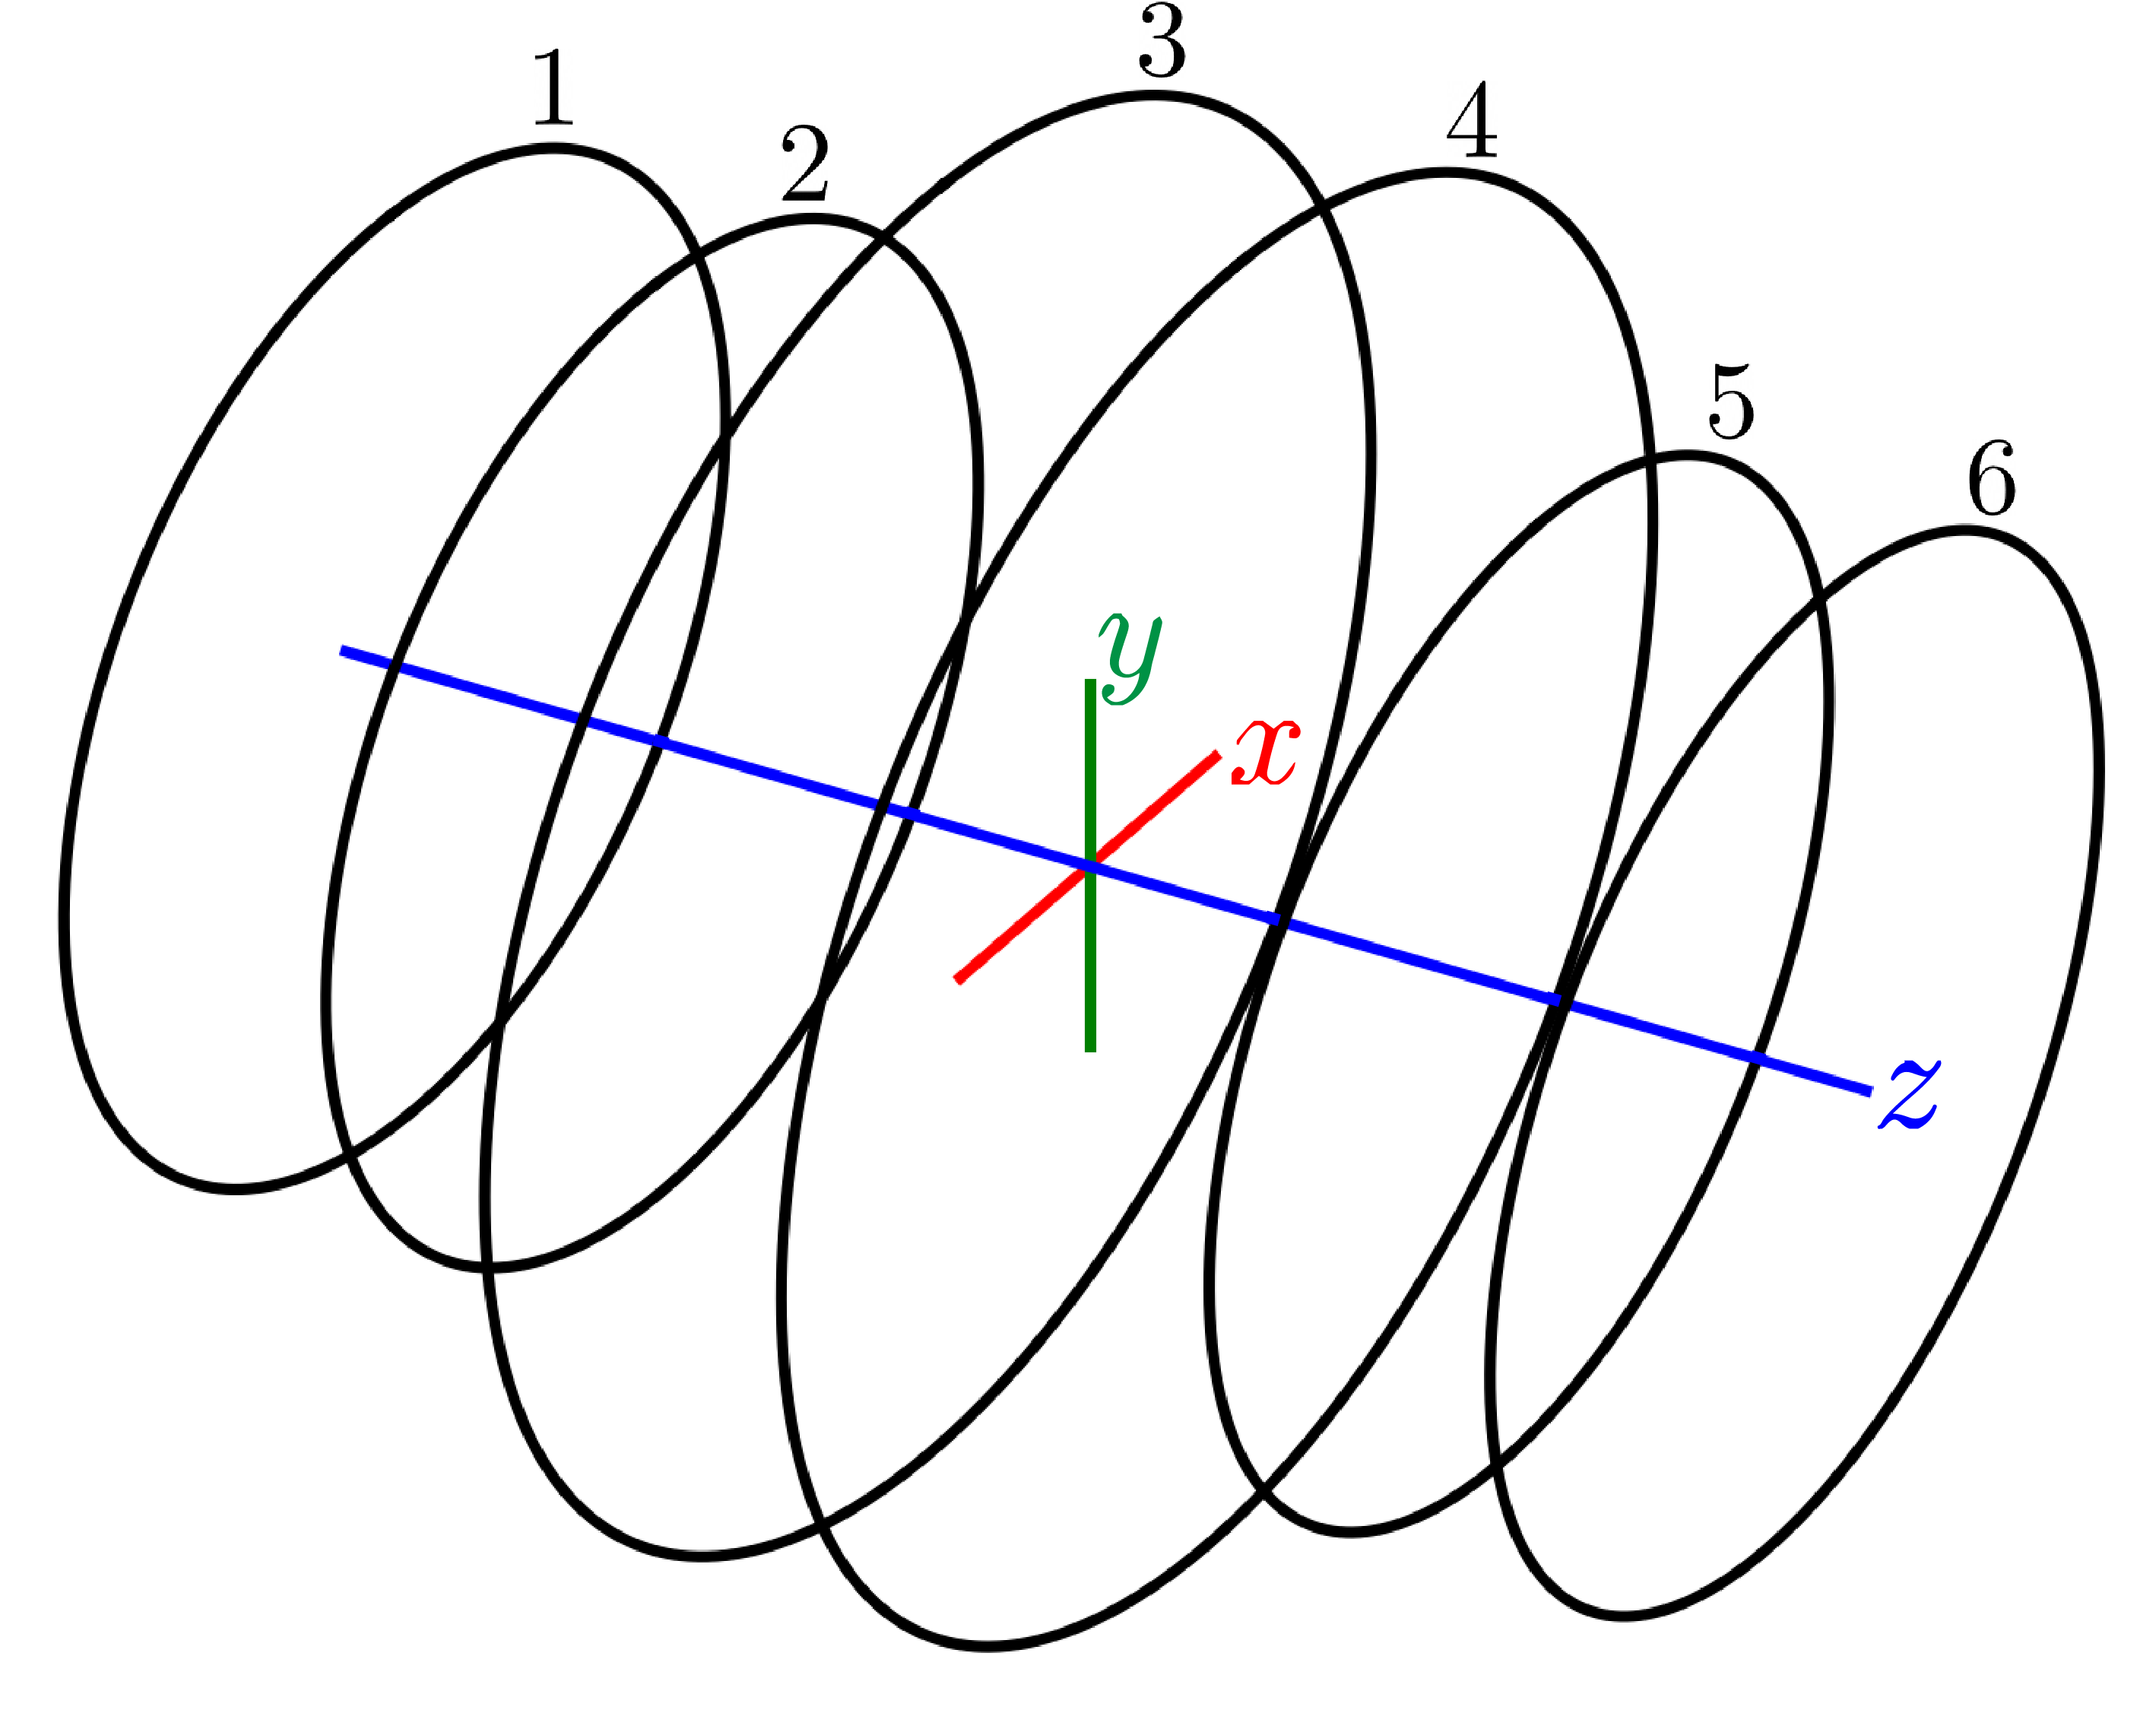
\includegraphics[width=1\textwidth]{figs/Chapter-4/230512_trap10_coils.png}
        \label{fig:chap4-trap10-coils} 
    \end{minipage}
    \par
    \centering
    \begin{minipage}{0.7\textwidth}
        \centering
        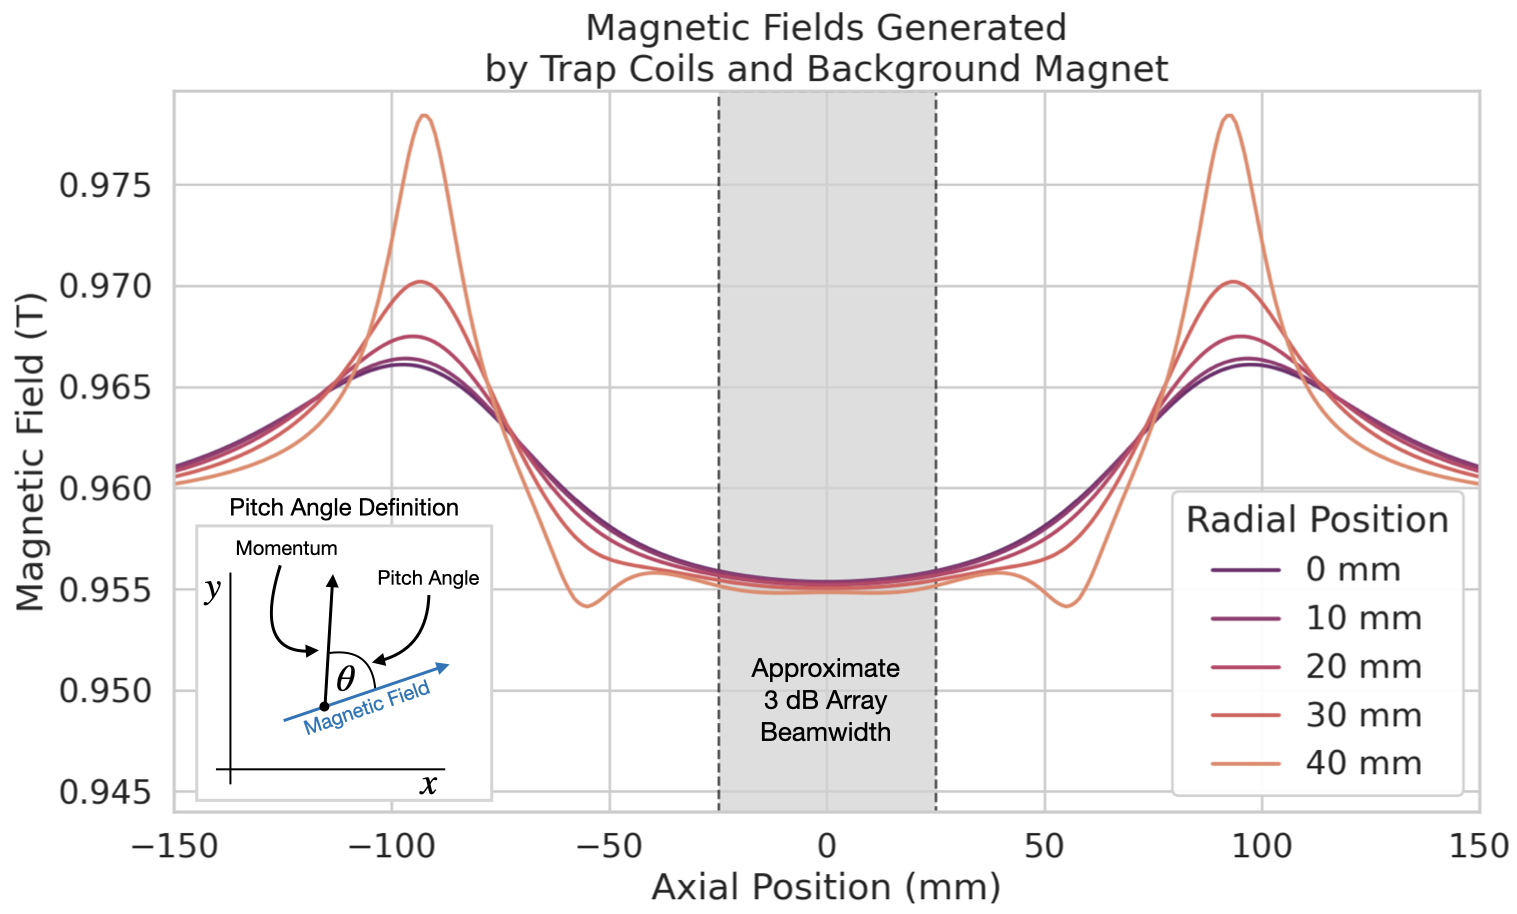
\includegraphics[width=1\textwidth]{figs/Chapter-4/230214_annotate_trap_profile_image.001.png}
    \end{minipage}
    \captionof{figure}{The geometry and parameters of the coils used to simulate the FSCD magnetic trap in Kassiopeia. Some axial profiles of the magnetic trap at different radial positions are shown to demonstrate the shape of the magnetic field and trap depth as a function of position. Calulation of the magnetic field profiles was graciously done by Ren\'{e} Reimann.}
    \label{fig:chap4-trap10-coils}
\end{table}

The depth of the FSCD trap is approximately 10~mT when measured along the central axis, which is sufficient to trap electrons with pitch angles as small as $84^\circ$. The trap depth influences the efficiency of the experiment by directly controlling the range of electron pitch angles that can be trapped. If a higher fraction of pitch angles are trapped, in principle, more decay events can be observed. However, the signals from electrons with small pitch angles are significantly harder to detect in the FSCD than large pitch angles, which increases the likelihood of not detecting the first track of the CRES event and harms the energy resolution of the experiment. 

The steepness of the trap walls as well as non-uniformities in the magnetic field contribute to the total energy resolution of the CRES measurement by causing uncertainty in the relationship between an electron's kinetic energy and its cyclotron frequency. When an electron is trapped, it oscillates back and forth along the trap z-axis (see Figure \ref{fig:chap4-trap10-coils}) unless it has a pitch angle of exactly $90^\circ$ \cite{p8pheno}. As the electron is reflected from the trap walls it experiences a change in the total magnetic field, which causes a modulation in the cyclotron frequency. This change in magnetic field from the trap introduces a correlation between the pitch angle and kinetic energy parameters of the electron that can reduce energy resolution. In order to mitigate this effect it is important to make the trap walls as steep as possible. 

%\begin{figure}[htbp]
%    \centering
%    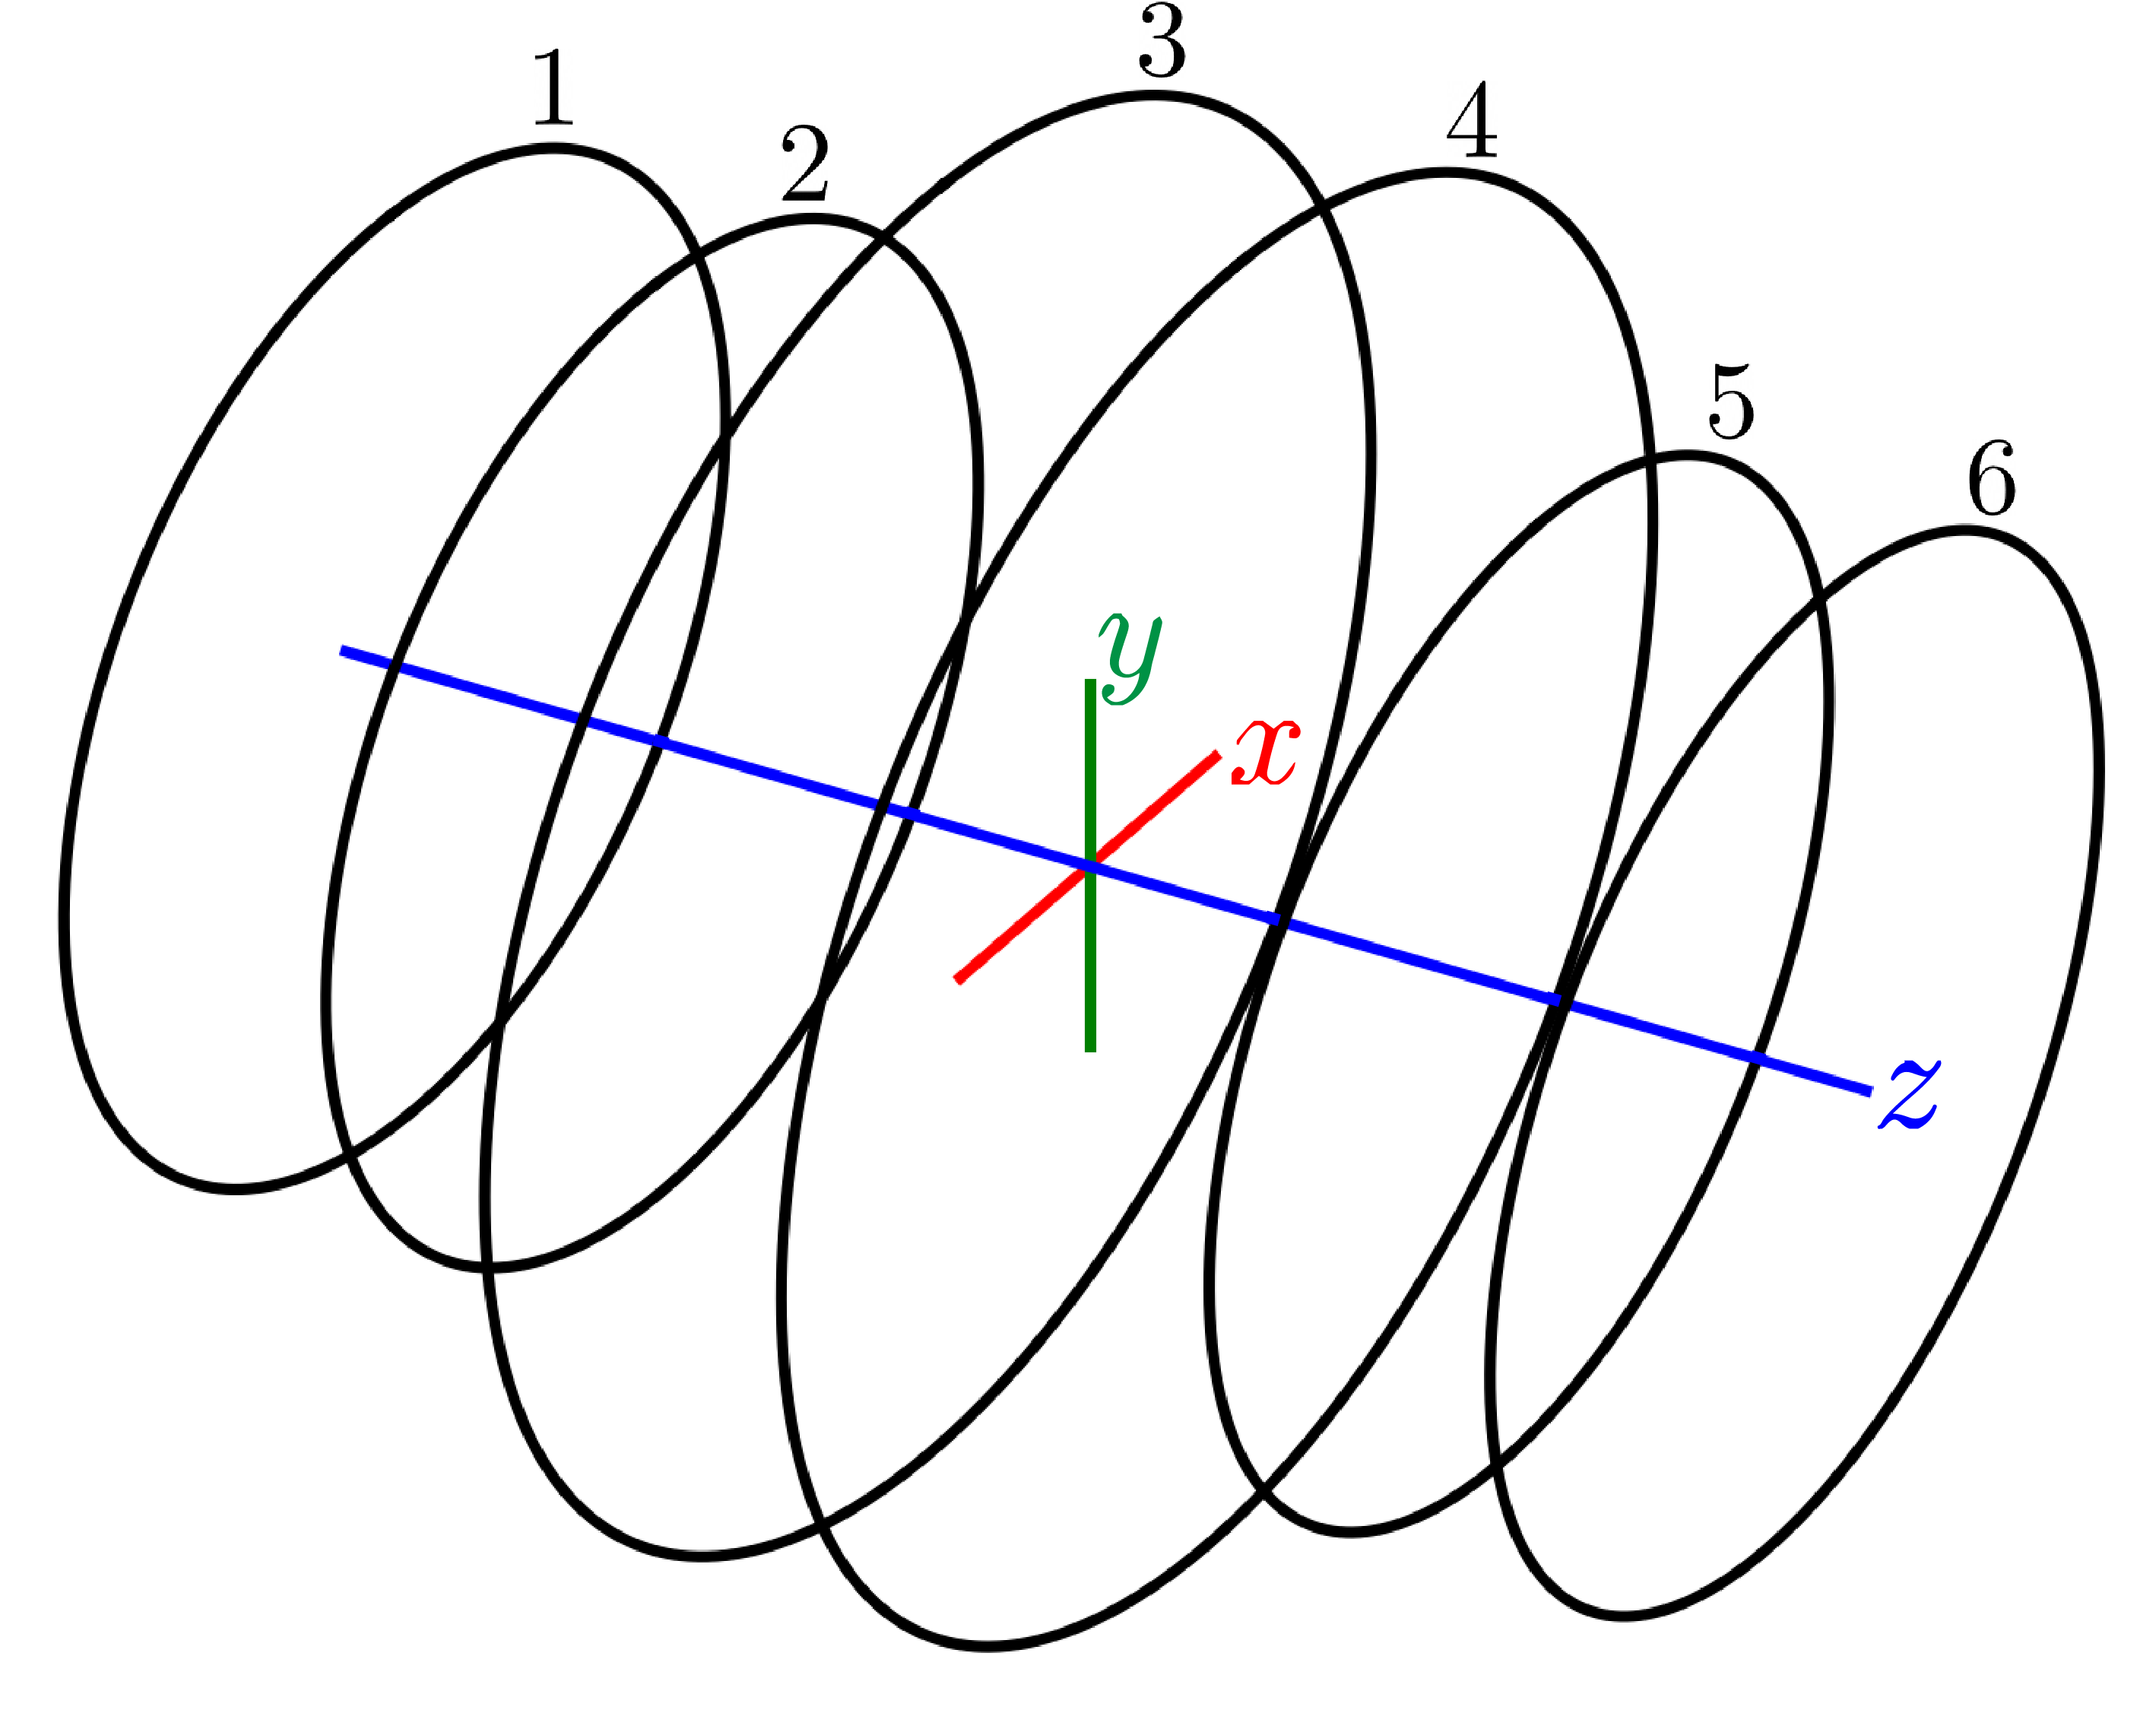
\includegraphics[width=0.5\textwidth]{figs/Chapter-4/230512_trap10_coils.png}
%    \caption{Caption}
%    \label{fig:chap4-trap10-coils}
%\end{figure}


%\begin{figure}[htbp]
%    \centering
%    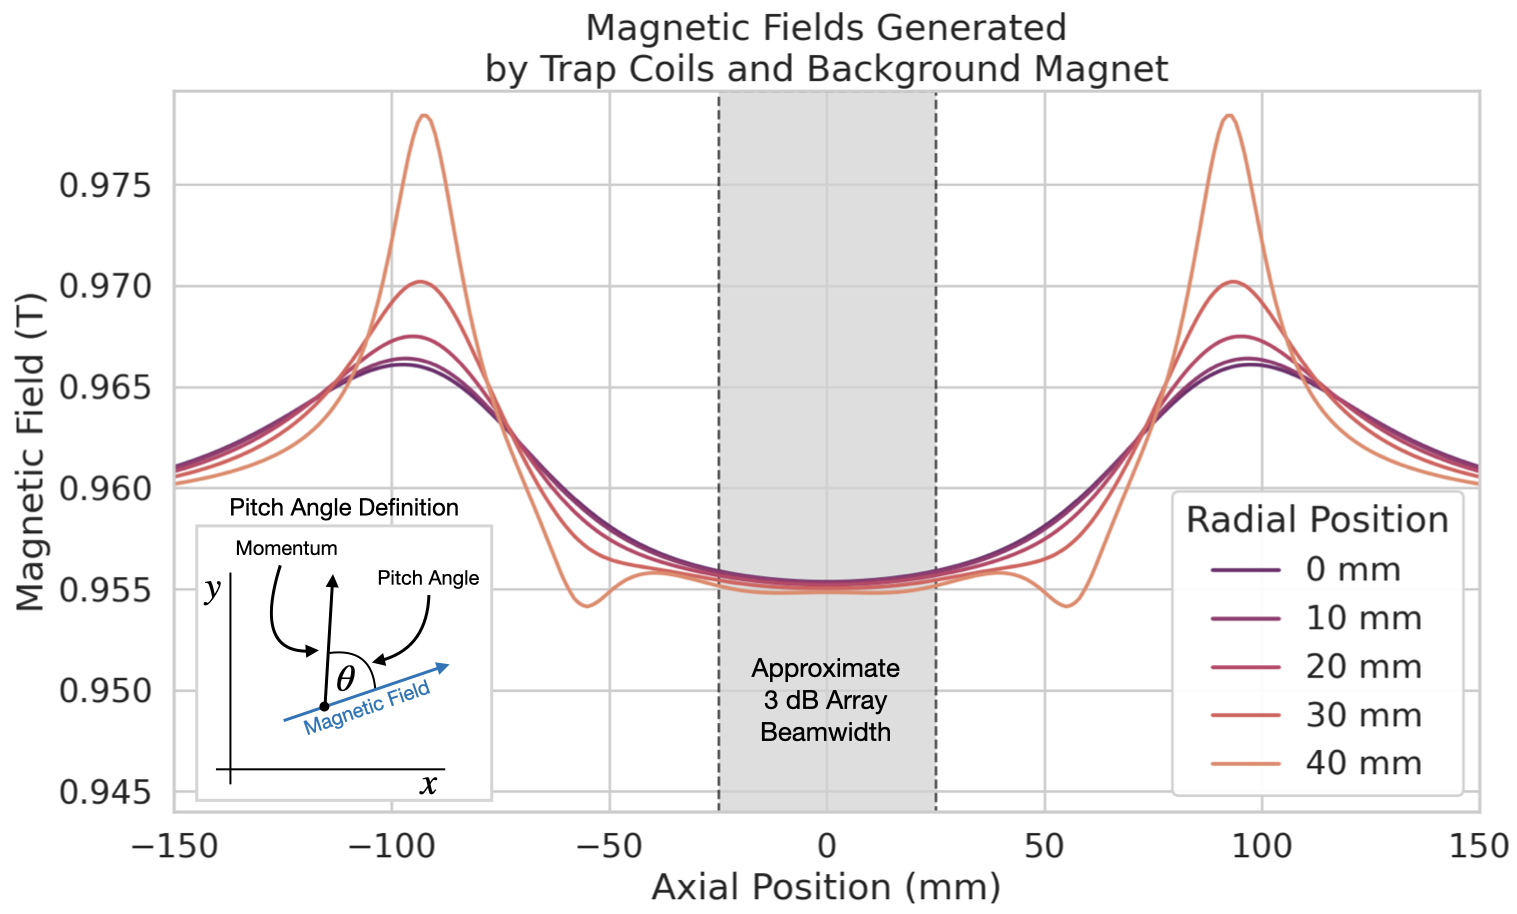
\includegraphics[width=0.7\textwidth]{figs/Chapter-4/230214_annotate_trap_profile_image.001.png}
%    \caption{Profiles of the magnetic fields produced by a prototype magnetic trap and background magnet designed for the FSCD experiment.}
%    \label{fig:chap4-mag-trap-profile}
%\end{figure}

\subsubsection*{Particle Trajectory Solutions}

The magnetic fields solved by direct integration of the coil current densities are used to calculate the trajectories of electrons based on user specified initial conditions. Various statistical distributions are available, which can be sampled to replicate realistic event statistics. These include uniform, Gaussian, and Lorentzian distributions among others. In general, an electron has six kinematic parameters that define its trajectory, which are the three-dimensional coordinates of the initial position and the three components of the electron's momentum vector. However, when simulating CRES events it is common to parameterize the electron's trajectory in terms of the initial position, kinetic energy, pitch angle, and initial direction of the component of the electron's momentum perpendicular to the magnetic field. This parameterization is completely equivalent to specifing the starting position and momentum vectors. 

From the initial parameters of the electron and the magnetic field, Kassiopeia solves for the trajectory of the electron. The direct approach proceeds by solving the motion of the electron using the Lorentz force equation, which takes the form of a set of differential equations 
\begin{align}
    \frac{d\mathbf{r}}{dt}&=\frac{\mathbf{p}}{\gamma m}\\
    \frac{d\mathbf{p}}{dt}&=e(\mathbf{E}+\frac{\mathbf{p}\times\mathbf{B}}{\gamma m}),
\end{align}
where $\mathbf{r}$ is the position of the electron, $\mathbf{p}$ is the electron's momentum, $e$ is the charge of the electron, $m$ is the electron's mass, and $\gamma$ is the relativistic Lorentz term. % To account for kinetic energy losses from radiation, Kassiopeia includes an additional term in the momentum differential equation, which calculates the change in the electron's momentum induced by synchrotron radiation.
Kassiopeia solves this pair of differential equations using numerical integration, however, the exact trajectory can be computationally intensive to solve. If the adiabatic approximation can be applied, then Kassiopeia can make use of a simpler set of equations that can be more readily solved numerically. 

\begin{figure}[htbp]
    \centering
    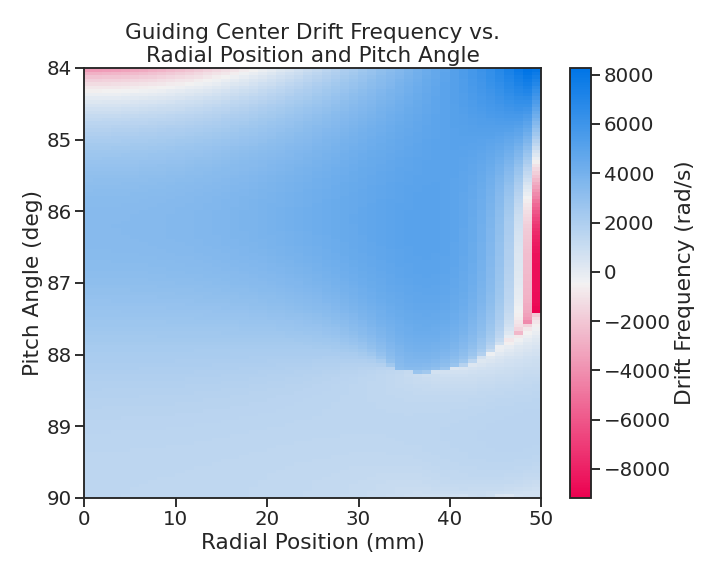
\includegraphics[width=0.6\textwidth]{figs/Chapter-4/230220_gradb_drift_frequencies.png}
    \caption{A map of the average $\nabla B$-drift frequency for electrons trapped in the prototype FSCD trap shown in Figure \ref{fig:chap4-trap10-coils}. Negative drift frequencies indicate electrons that are drifting opposite to the standard direction, which means that they are close to escaping the magnetic trap.}
    \label{fig:chap4-gradb-drift-frequency-map}
\end{figure}

Though Kassiopeia is not directly capable of simulating the cyclotron radiation, it is an invaluable CRES simulation tool. With Kassiopeia it is possible to test the efficiency of a particular trap design, and analyze features of the electron trajectories that are important to the position, track, and event reconstruction (see Section \ref{sec:chap4-pter}). An example is the analysis of the average $\nabla B$-drift frequency as a function of the electrons radial position and pitch angle in the FSCD trap (see Figure \ref{fig:chap4-gradb-drift-frequency-map}). Radial gradients in the trap cause the guiding center of the electron to drift around the center of the magnetic trap with an average frequency on the order of $10^3$~rad/s. This frequency, while slow compared to the length of a typical CRES time-slice, is large enough to cause a significant loss in efficiency of certain signal reconstruction algorithms. Therefore, it is important to model the drift of the electron in the reconstruction algorithm in order to mitigate the effects of this motion on the reconstruction.

\subsection{Locust}

The Locust\footnote{\url{https://github.com/project8/locust_mc/tree/master}} software package \cite{p8locustpaper} is the primary simulation tool developed and used by the Project 8 collaboration for CRES experiments. Locust simulates the responses of antennas and receiver electronics chain to rapidly time-varying electric fields using a flexible approach that allows one to choose from a variety of electric field sources and antennas. Similarly, one can simulate the receiver chain using a series of modular generators that include standard signal processing operations such as down-mixing and fast Fourier transforms (FFT). Since the primary focus of this chapter is the application of Locust to analyses of the FSCD, I shall describe only the most relevant aspects of the software rather than provide a comprehensive description.

\subsubsection*{Cyclotron Radiation Field Solutions}

Simulating CRES events in the FSCD requires one to calculate the electric fields produced by the acceleration of the electron. In the general case, this can be a complicated computation, due to back-reaction forces on the electron. However, in the case of the FSCD it is possible to ignore such effects and approximate the electron as radiating into a free-space environment. 

The equations that describe the EM fields from a relativistic moving point particle are the Li\'{e}nard-Wiechert equations \cite{lw_potential_1,lw_potential_2}, which are obtained by differentiating the Li\'{e}nard-Wiechert potentials. In their full form, the Li\'{e}nard-Wiechert field equations are
\begin{align}
    \bm{E} &=e\left[\frac{\hat{n}-\bm{\beta}}{\gamma^2(1-\bm{\beta}\cdot\hat{n})^3|\bm{R}|^2}\right]_{t_\textrm{r}}
      +\frac{e}{c}\left[\frac{\hat{n}\times[(\hat{n}-\bm{\beta})\times\dot{\bm{\beta}}]}{(1-\bm{\beta}\cdot\hat{n})^3|\bm{R}|}\right]_{t_\textrm{r}}\label{eq:chap4-lw-eqn-efield}\\
    \bm{B} &= \left[\hat{n}\times \bm{E}\right]_{t_\textrm{r}},
\end{align}
where $e$ is the charge of the particle, $\hat{n}$ is the unit vector pointing from the particle to the position where the fields are calculated, $\bm{\beta}$ and $\dot{\bm{\beta}}$ are the velocity and acceleration of the particle divided by the speed of light ($c$), $\bm{R}$ is the distance from the particle to the field calculation position, and $\gamma$ is the relativistic Lorentz term. The subscript $t_\mathrm{r}$ indicates that the equations are evaluated at the retarded time so that the time-delay from the travel time of the electromagnetic radiation is taken into account. 

The only required input to calculate the electric field at the position of an FSCD antenna is the velocity and acceleration of the electron, which can be obtained from Kassiopeia simulations. Therefore, when simulating a CRES event Locust first runs a Kassiopeia simulation of the electron and subsequently calculates the electric field incident on the antenna. This requires one to calculate the retarded time. The retarded time corresponds to the time that a photon, which has just arrived at an antenna at the space-time position $(t,\bm{r})$, was actually emitted by the electron at the space-time position of $(t_\mathrm{r}, \bm{r}_e(t_\mathrm{r}))$. To calculate the retarded time one solves
\begin{equation}
    c(t-t_\mathrm{r}) = |\bm{r}-\bm{r}_e(t_\mathrm{r})|,
    \label{eq:chap4-ret-time-condition}
\end{equation}
where the distance traveled by the photon between the measurement and retarded times is equal to the distance between the antenna and the electron at the retarded time. Locust solves Equation \ref{eq:chap4-ret-time-condition} using root finding algorithm to calculate the retarded time, which yields the electric field emitted by the electron, at the position of each antenna in the FSCD array.

\subsubsection*{Antenna Response Modeling}

The electric field solutions are used to calculate the resulting voltages produced in the antenna. However, direct simulation of the antenna itself is computationally expensive, since it requires modeling the complex interactions of the electron's electric fields with charge carriers in the antenna. Direct simulation of the antenna in Locust is avoided by modeling the antenna response using the antenna factor, or antenna transfer function. The antenna factor defines the voltage produced in the antenna terminal for an incident electric field \cite{balanis2015antenna},
\begin{equation}
    A_\mathrm{F}=\frac{V}{|\bm{E}|},
\end{equation}
where V is the voltage and $|\bm{E}|$ is the magnitude of the incident electric field. To obtain the antenna factor for the antennas developed for the FSCD Project 8 employs Ansys HFSS. HFSS is a commercially available finite element method electromagnetic solver widely used throughout the antenna engineering industry \cite{hfss}. HFSS is capable of calculating the antenna factor and gain patterns for complex antenna designs and outputting the resulting quantities in the form of a text file that can be used as a configuration input to Locust. 

The antenna factor defines the steady-state response of the antenna to electromagnetic plane waves in the frequency-domain. Since the antenna response is calculated in the time-domain Locust models the antenna as a linear time-invariant system \cite{lti_theory_wiki}. In this formalism the response of the system to the driving force is given by 
\begin{equation}
    y[n] = h\ast x=\sum_{k}{h[k]x[n-k]},
\end{equation}
where $y[n]$ is the discretely sampled response, $x$ is the driving force stimulus, and $h$ is the finite impulse response (FIR) filter. When applied to the FSCD array, this formalism calculates the voltage time-series produced in each antenna by convolving the electric field time-series with the antenna FIR filter, which is obtained by performing an inverse Fourier transform on the transfer function from HFSS. 

\subsubsection*{Radio-frequency Receiver and Signal Processing}

After obtaining the voltage time-series by computing the electron trajectory and antenna response, Locust simulates the signal processing performed by the RF receiver chain. The simulated Locust receiver chain includes all operations that would be performed by the RF hardware (see Figure \ref{fig:chap4-locust-receiver-chain}). 

\begin{figure}[htbp]
    \centering
    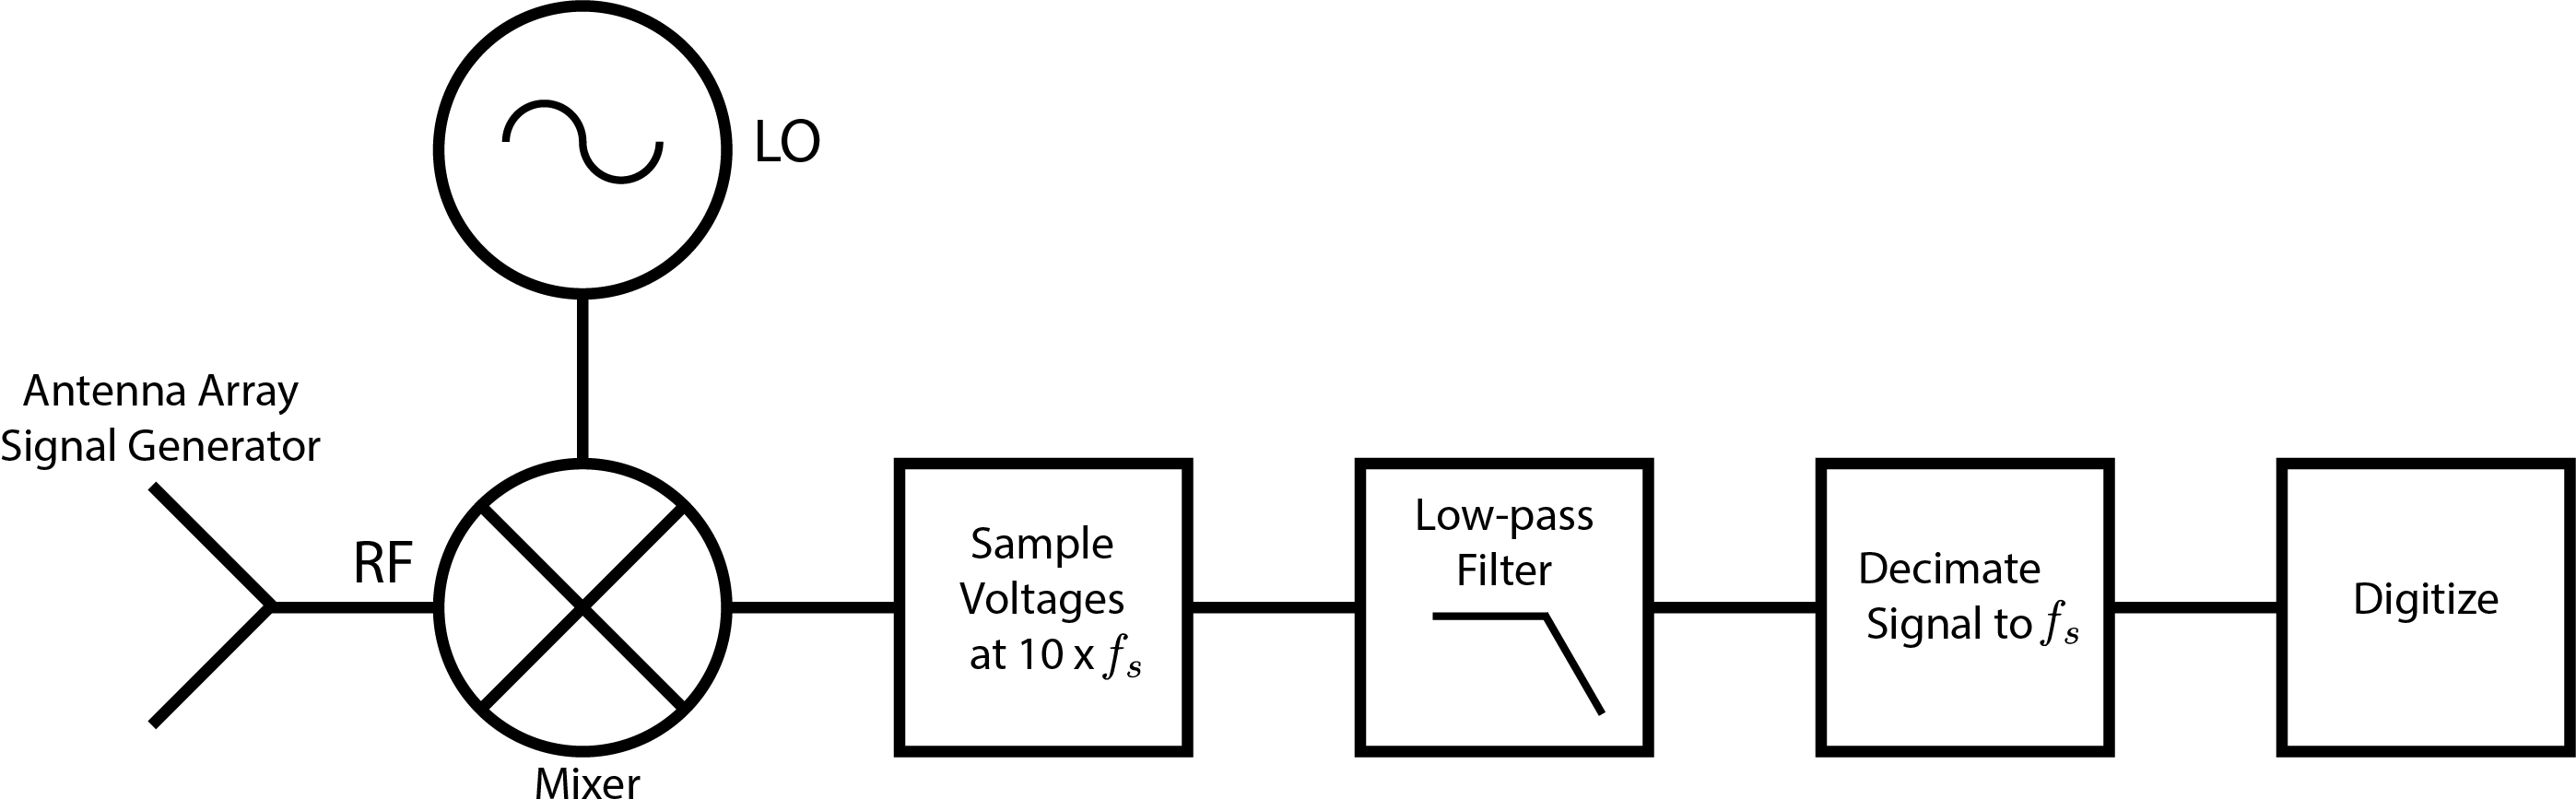
\includegraphics[width=0.85\textwidth]{figs/Chapter-4/230511_locust_receiver_chain.png}
    \caption{The receiver chain used by Locust when simulating CRES events in the FSCD.}
\label{fig:chap4-locust-receiver-chain}
\end{figure}

Frequency down-conversion reduces the digitization bandwidth required to read-out CRES data. According to the Nyquist sampling theorem \cite{nyquist_sampling}, the minimal sampling rate that guarantees no information loss for a signal with a bandwidth $\Delta f$ is given by
\begin{equation}
    f_{\textrm{Nyq}}=2\Delta f.
\end{equation}
The total bandwidth for CRES events ranges from 0 to 26~GHz in a $0.95$~T magnetic field; therefore, direct digitization of CRES signals from the FSCD would require sampling frequencies greater than $50$~GHz, which is infeasible for a real experiment. However, one need only measure the shape of the spectrum in the last 100~eV, which corresponds to a frequency bandwidth of 5~MHz, to effectively measure the neutrino mass. 

Down-conversion is a technique for reducing the base frequencies of signals in a bandwidth given by $[f_\textrm{LO},f_\textrm{LO}+\Delta f]$ to the bandwidth $[0, \Delta f]$, by performing the following multiplication
\begin{equation}
    x(t)\rightarrow x(t)e^{-2\pi f_\textrm{LO}}.
\end{equation}
The signal, $x(t)$, is multiplied by a sinusoidal signal with frequency $f_\textrm{LO}$ to reduce the absolute frequencies of the signals in the bandwidth. In the FSCD, this allows one to detect events in the last 100~eV of the tritium spectrum, while sampling the data far below 50~GHz. The standard bandwidth used in the FSCD is 200~MHz, which allows for higher frequency resolution than the minimum sampling frequency for 100~eV of energy bandwidth.

Directly simulating down-conversion with a frequency multiplication in Locust requires sampling the electric fields at each antenna in the FSCD array with a period of $\approx20$~ps, which is extremely slow computationally. To avoid this, Locust performs the down-conversion by intentionally under-sampling the electric fields with a frequency of 2~GHz. Sampling below the Nyquist limit causes the higher frequency components of the CRES signal to alias, however, Locust can remove these aliased frequency peaks using a combination of low-pass filtering and decimation to recreate frequency down-conversion. After filtering and decimation, Locust simulates digitization by an 8-bit digitizer at a sampling frequency of 200~MHz to recreate the conditions of the FSCD. The voltage offset and digitizer range must be configured by the user based on the characteristics of the simulation. 

\subsubsection*{Data}

The output of Locust simulations for the FSCD primarily consists of two data files. The first is the electron trajectory information calculated by Kassiopiea, which is output in the form of a \texttt{.root} file \cite{root}. This file contains important kinematic information about the electron such as its position and pitch angle as a function of time. The other file is produced by Locust and contains the digitized signals acquired from each antenna in the array. The Locust output files conform to the Monarch specification\footnote{https://github.com/project8/monarch} developed by Project 8, which is based on the commonly used HDF5 file format, and matches the format of the files produced by the Project 8 data acquisition software. This makes it possible to use the same data analysis code to analyze both simulated and real data.

\subsection{CRESana}
\label{sec:chap4-cresana}

Locust is the primary simulation tool used by Project 8 in the development and simulation of the FSCD. However, simulations of CRES events in larger antenna arrays ($\geq100$ antennas) can take several hours to complete, which is prohibitively long when one is performing a sensitivity analysis and optimization. One reason for Locust's slow operation is that the electric fields from the electron must be solved numerically for each time-step for all antennas in the array. These numerical solutions allow Locust to accurately simulate the electric fields from arbitrarily complicated electron trajectories at the cost of more computations and slower simulations. Therefore, an additional simulation tool that sacrifices the accuracy of numerical approaches for computational efficiency is a useful tool for studying large antenna array experiments.

Recently, Project 8 has developed a new simulations package called CRESana\footnote{\url{https://github.com/MCFlowMace/CRESana}}, specifically designed to perform analytical simulations of antenna-based CRES experiments. CRESana provides a significant increase in simulation speed by using well-justified analytical approximations of the electrons motion and electric fields in a magnetic trap. The electric fields and signals generated by CRESana are consistent with theoretical calculations of the electron's radiation, and are tested for accuracy using well-known test-case simulations and consistency checks. 

\section{Signal Detection and Reconstruction Techniques for Antenna Array CRES}
\label{sec:chap4-pter}

\subsubsection*{Antenna Array CRES Signal Reconstruction}

%A robust set of FSCD simulation tools are vital to the development of the analysis algorithms necessary for antenna array CRES to succeed.
Antenna array CRES requires one to use the multichannel time-series obtained by digitizing the array to estimate the starting kinetic energies of electrons produced in the magnetic trap using CRES signal reconstruction algorithm. This procedure consists of a multi-stage process of detecting a CRES signal followed by an estimation of the electron's parameters.

Antenna array CRES requires a significantly different approach to signal reconstruction than previous Project 8 experiments. In Phases I and II, CRES was performed using a waveguide gas cell directly integrated into a waveguide transmission line. The transmission line efficiently propagates the cyclotron radiation along its length to an antenna at the ends of the waveguide. However, with an antenna array the electron is radiating into free-space; therefore, the cyclotron radiation power collected by the array is directly proportional to the solid angle surrounding the electron that is covered with antennas. Because it is not practical to fully surround the magnetic trap with antennas, some of the cyclotron radiation power that would have been collected by the waveguide escapes into free-space. Furthermore, the power that is collected by the antenna array is split between every channel in the antenna array, which significantly lowers the signal-to-noise ratio (SNR) of CRES signals in a single antenna channel compared to a waveguide apparatus. Therefore, a suite of completely new signal reconstruction techniques are needed in order to perform CRES in the FSCD.

Changes to the approach to CRES signal reconstruction are also motivated by the scientific goals of Project 8. A measurement of the tritium beta-decay spectrum that is sensitive to neutrino masses as small as 40~meV requires that we measure the kinetic energies of individual electrons with a total energy broadening of 115~meV \cite{p8bayesian}. This resolution includes all sources of uncertainty in the electron's kinetic energy such as magnetic field inhomogeneities. This precise energy resolution is only achieved by an event-by-event signal reconstruction approach where the kinetic energies, pitch angles, and other parameters of the CRES events are estimated for individual electrons before constructing the beta-decay spectrum. 

The event-by-event approach is distinct from the analysis done for the Phase I and Phase II experiments, where the starting cyclotron frequency of the event was measured by analyzing the tracks formed by the electron's carrier in a time-frequency spectrogram. These frequencies were then combined into a frequency beta-spectrum, which was converted to the beta-decay energy spectrum using an ensemble approach that averaged over all other event parameters. The ensemble approach to signal reconstruction results in poor energy resolution because other kinematic parameters such as pitch angle change the cyclotron carrier frequency due to changes in the average magnetic field experience by the electron.

\subsubsection*{Components of Reconstruction: Signal Detection and Parameter Estimation}

CRES signal reconstruction is a two-step procedure consisting of signal detection followed by parameter estimation. In the former, one is concerned with identifying CRES signals in the data regardless of the signal parameters; whereas, in the latter one operates under the assumption that a signal is present and then estimates it's parameters. 

More formally, signal detection can be posed as a binary hypothesis test between the signal and noise data classes, and parameter estimation is a process of fitting a signal model to the observed data. While both of these are required for a complete reconstruction (see Figure \ref{fig:chap4-pter-pipeline}), the focus of my work and this chapter is on the signal detection aspect of antenna array CRES signal reconstruction.

\begin{figure}[htbp]
    \centering
    
\includegraphics[width=0.8\textwidth]{figs/Chapter-4/230108_deepfilter_paper_event_reconstruction_pipeline.png}
    \caption{A high-level diagram depicting the process of CRES event reconstruction. The first step consists of identifying the presence of a signal in the data. This step is necessary to avoid the danger of performing a reconstruction of a false event, which would constitute a background contribution to the tritium spectrum measured by CRES.}
    \label{fig:chap4-pter-pipeline}
\end{figure}

\subsubsection*{Detection Theory}


Signal detection is the process of deciding whether noisy data contains signal or noise, which can be posed as a statistical hypothesis test \cite{detection_theory}. For CRES signals, which are represented by signal vectors with added white Gaussian noise (WGN), one needs to choose between
\begin{align}
    \mathcal{H}_0:&\quad\bm{y}=\bm{\nu}\\
    \mathcal{H}_1:&\quad\bm{y}=\bm{x}+\bm{\nu},
\end{align}
where $\bm{y}$ is the CRES data vector, $\bm{\nu}$ is a sample of WGN, and $\bm{x}$ represents the CRES signal. The hypothesis that the data contains only noise is labeled $\mathcal{H}_0$ and the hypothesis that the data contains a signal is labeled $\mathcal{H}_1$.

For illustrative purposes, it is useful to study the case where only the first sample of data is used to distinguish between $\mathcal{H}_0$ and $\mathcal{H}_1$. The value of the first data sample is distributed according to two possible Gaussian distributions(see Figure \ref{fig:chap4-detection-threshold}). By setting a decision threshold on the value of this sample, one can choose the correct hypothesis with a probability given by the area underneath the probability distribution curves. A true positive corresponds to correctly identifying that the data contains signal; whereas, a true negative means that one has correctly identified the data as noise. The rate at which the detector performs a true positive classification is given by the green region underneath $p(\bm{y}[0];\mathcal{H}_0)$, and the rate at which the detector performs a true negative classification is given by the orange region underneath $p(\bm{y}[0];\mathcal{H}_1)$.
\begin{figure}[htbp]
    \centering
    \begin{subfigure}{0.48\textwidth}
        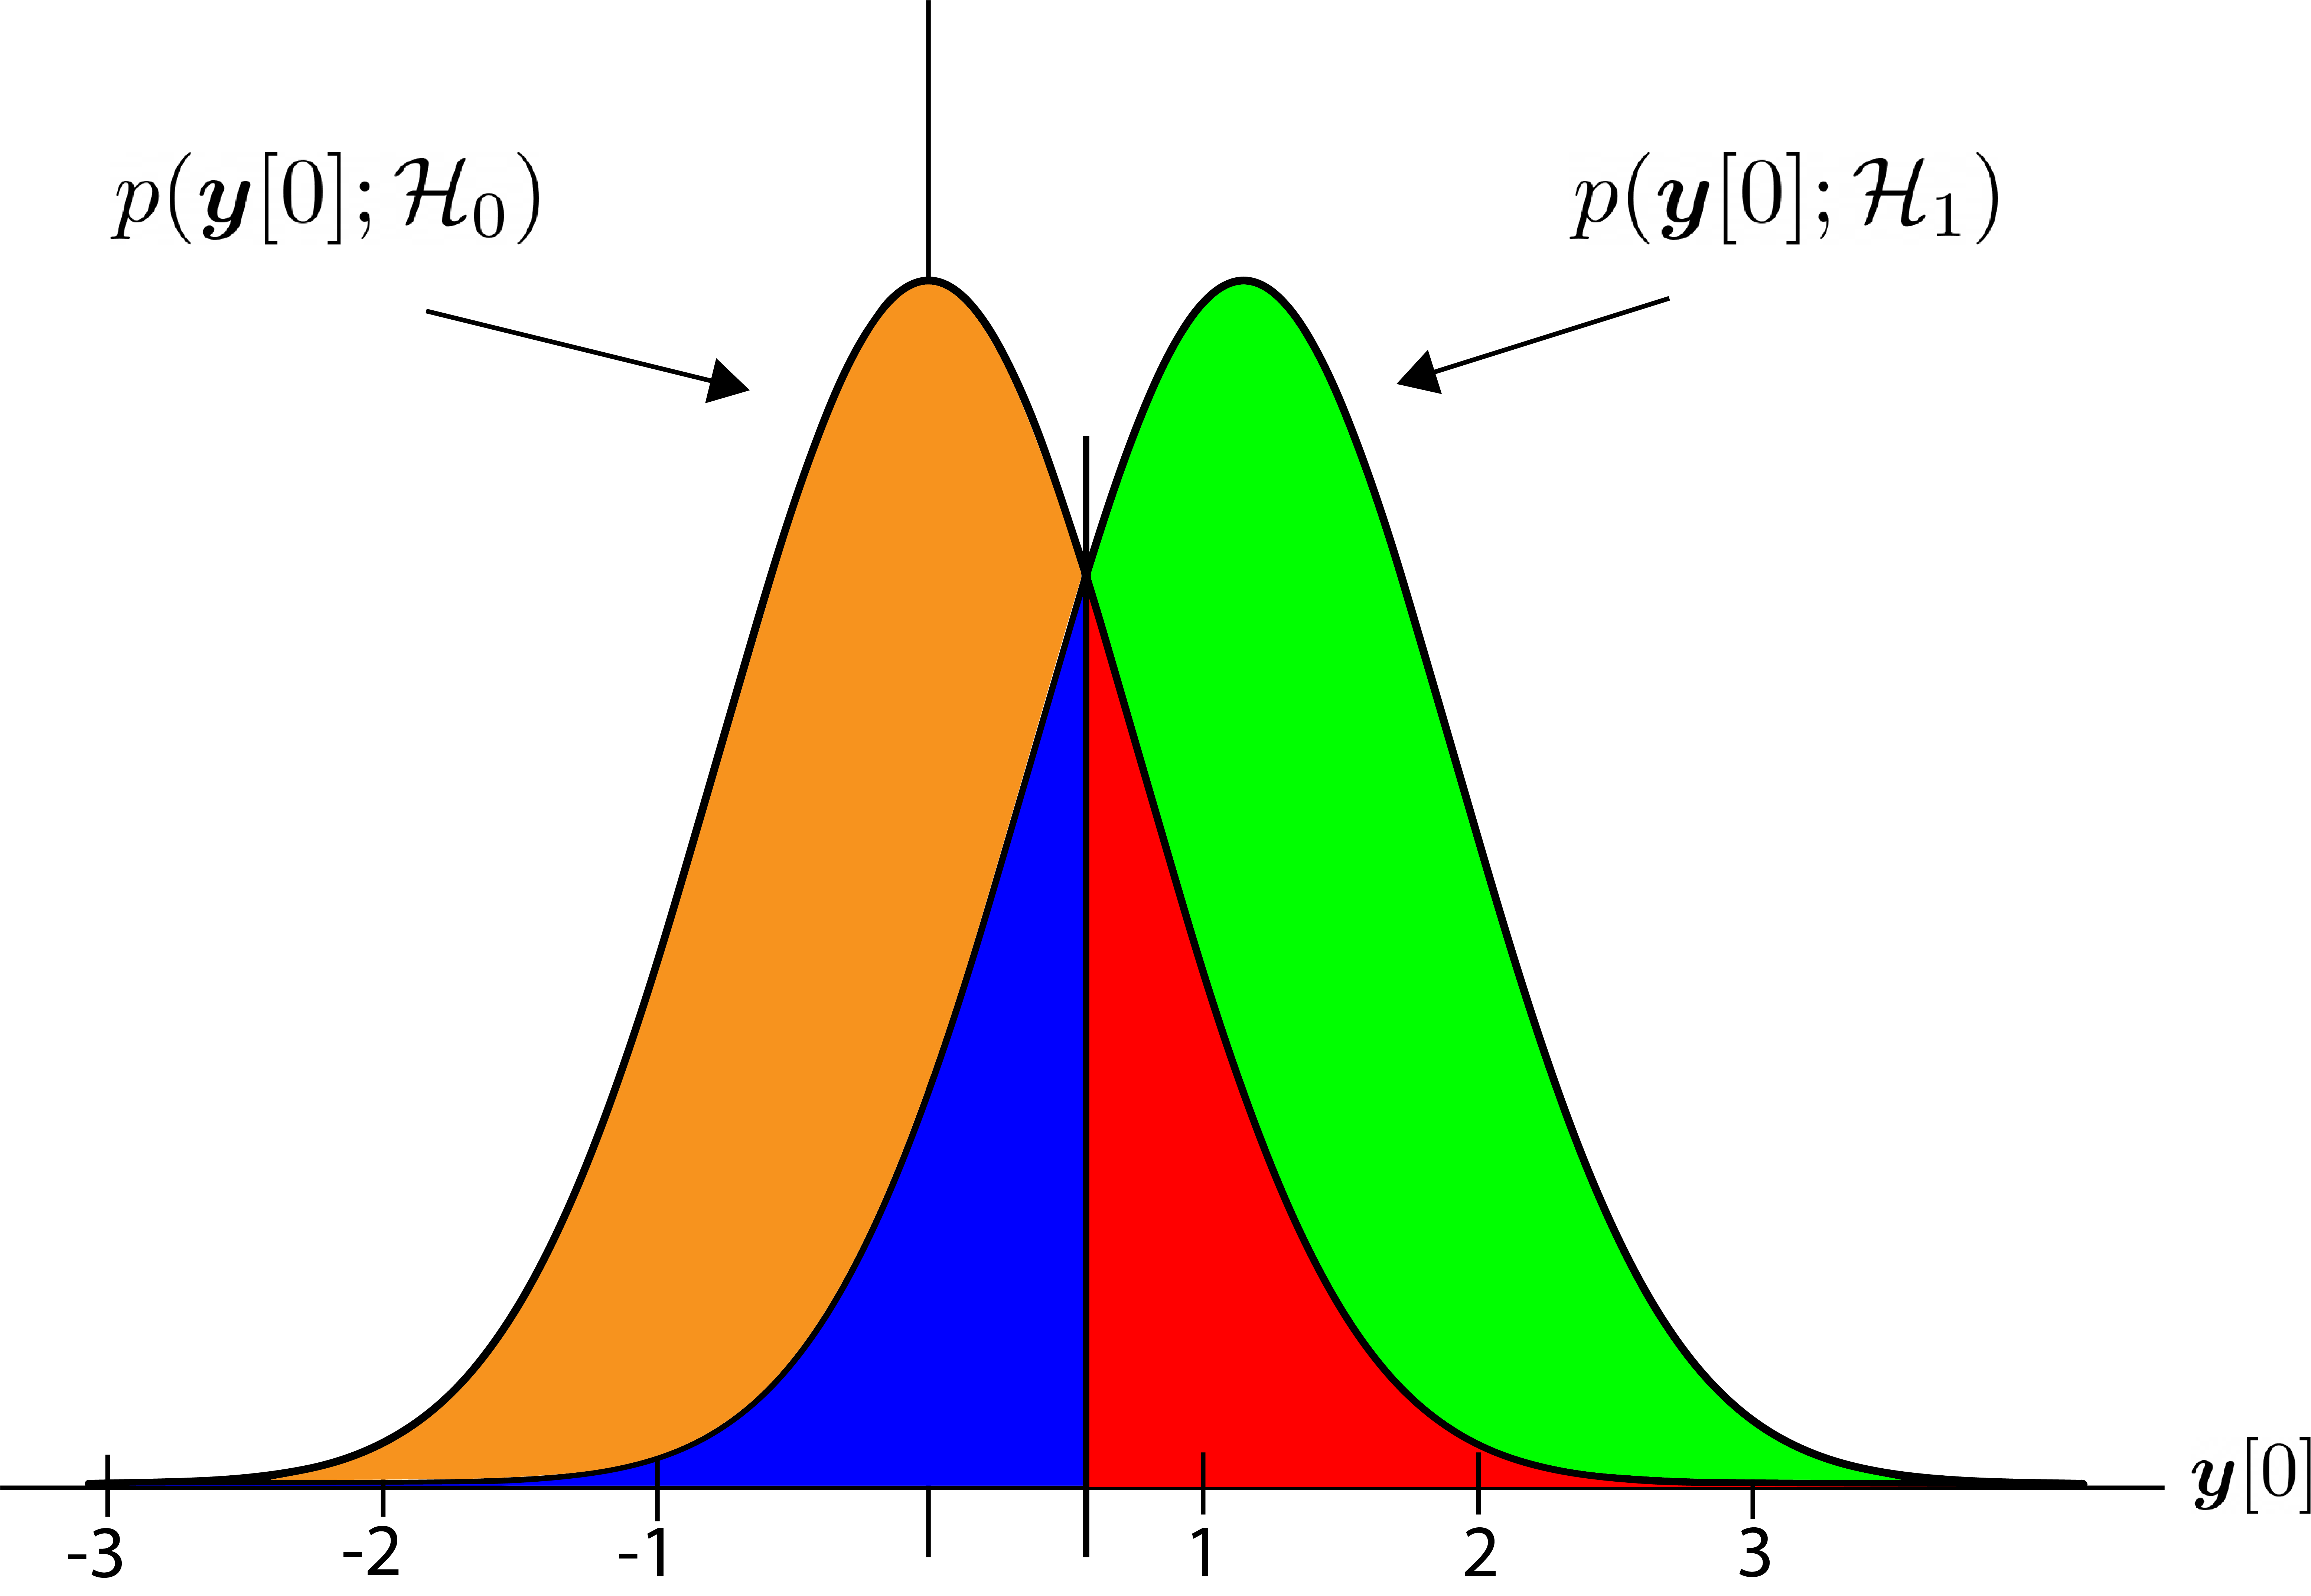
\includegraphics[width=\textwidth]{figs/Chapter-4/230523_detection_theory.png}
        \caption{}
    \end{subfigure}
    \hfill
    \begin{subfigure}{0.48\textwidth}
        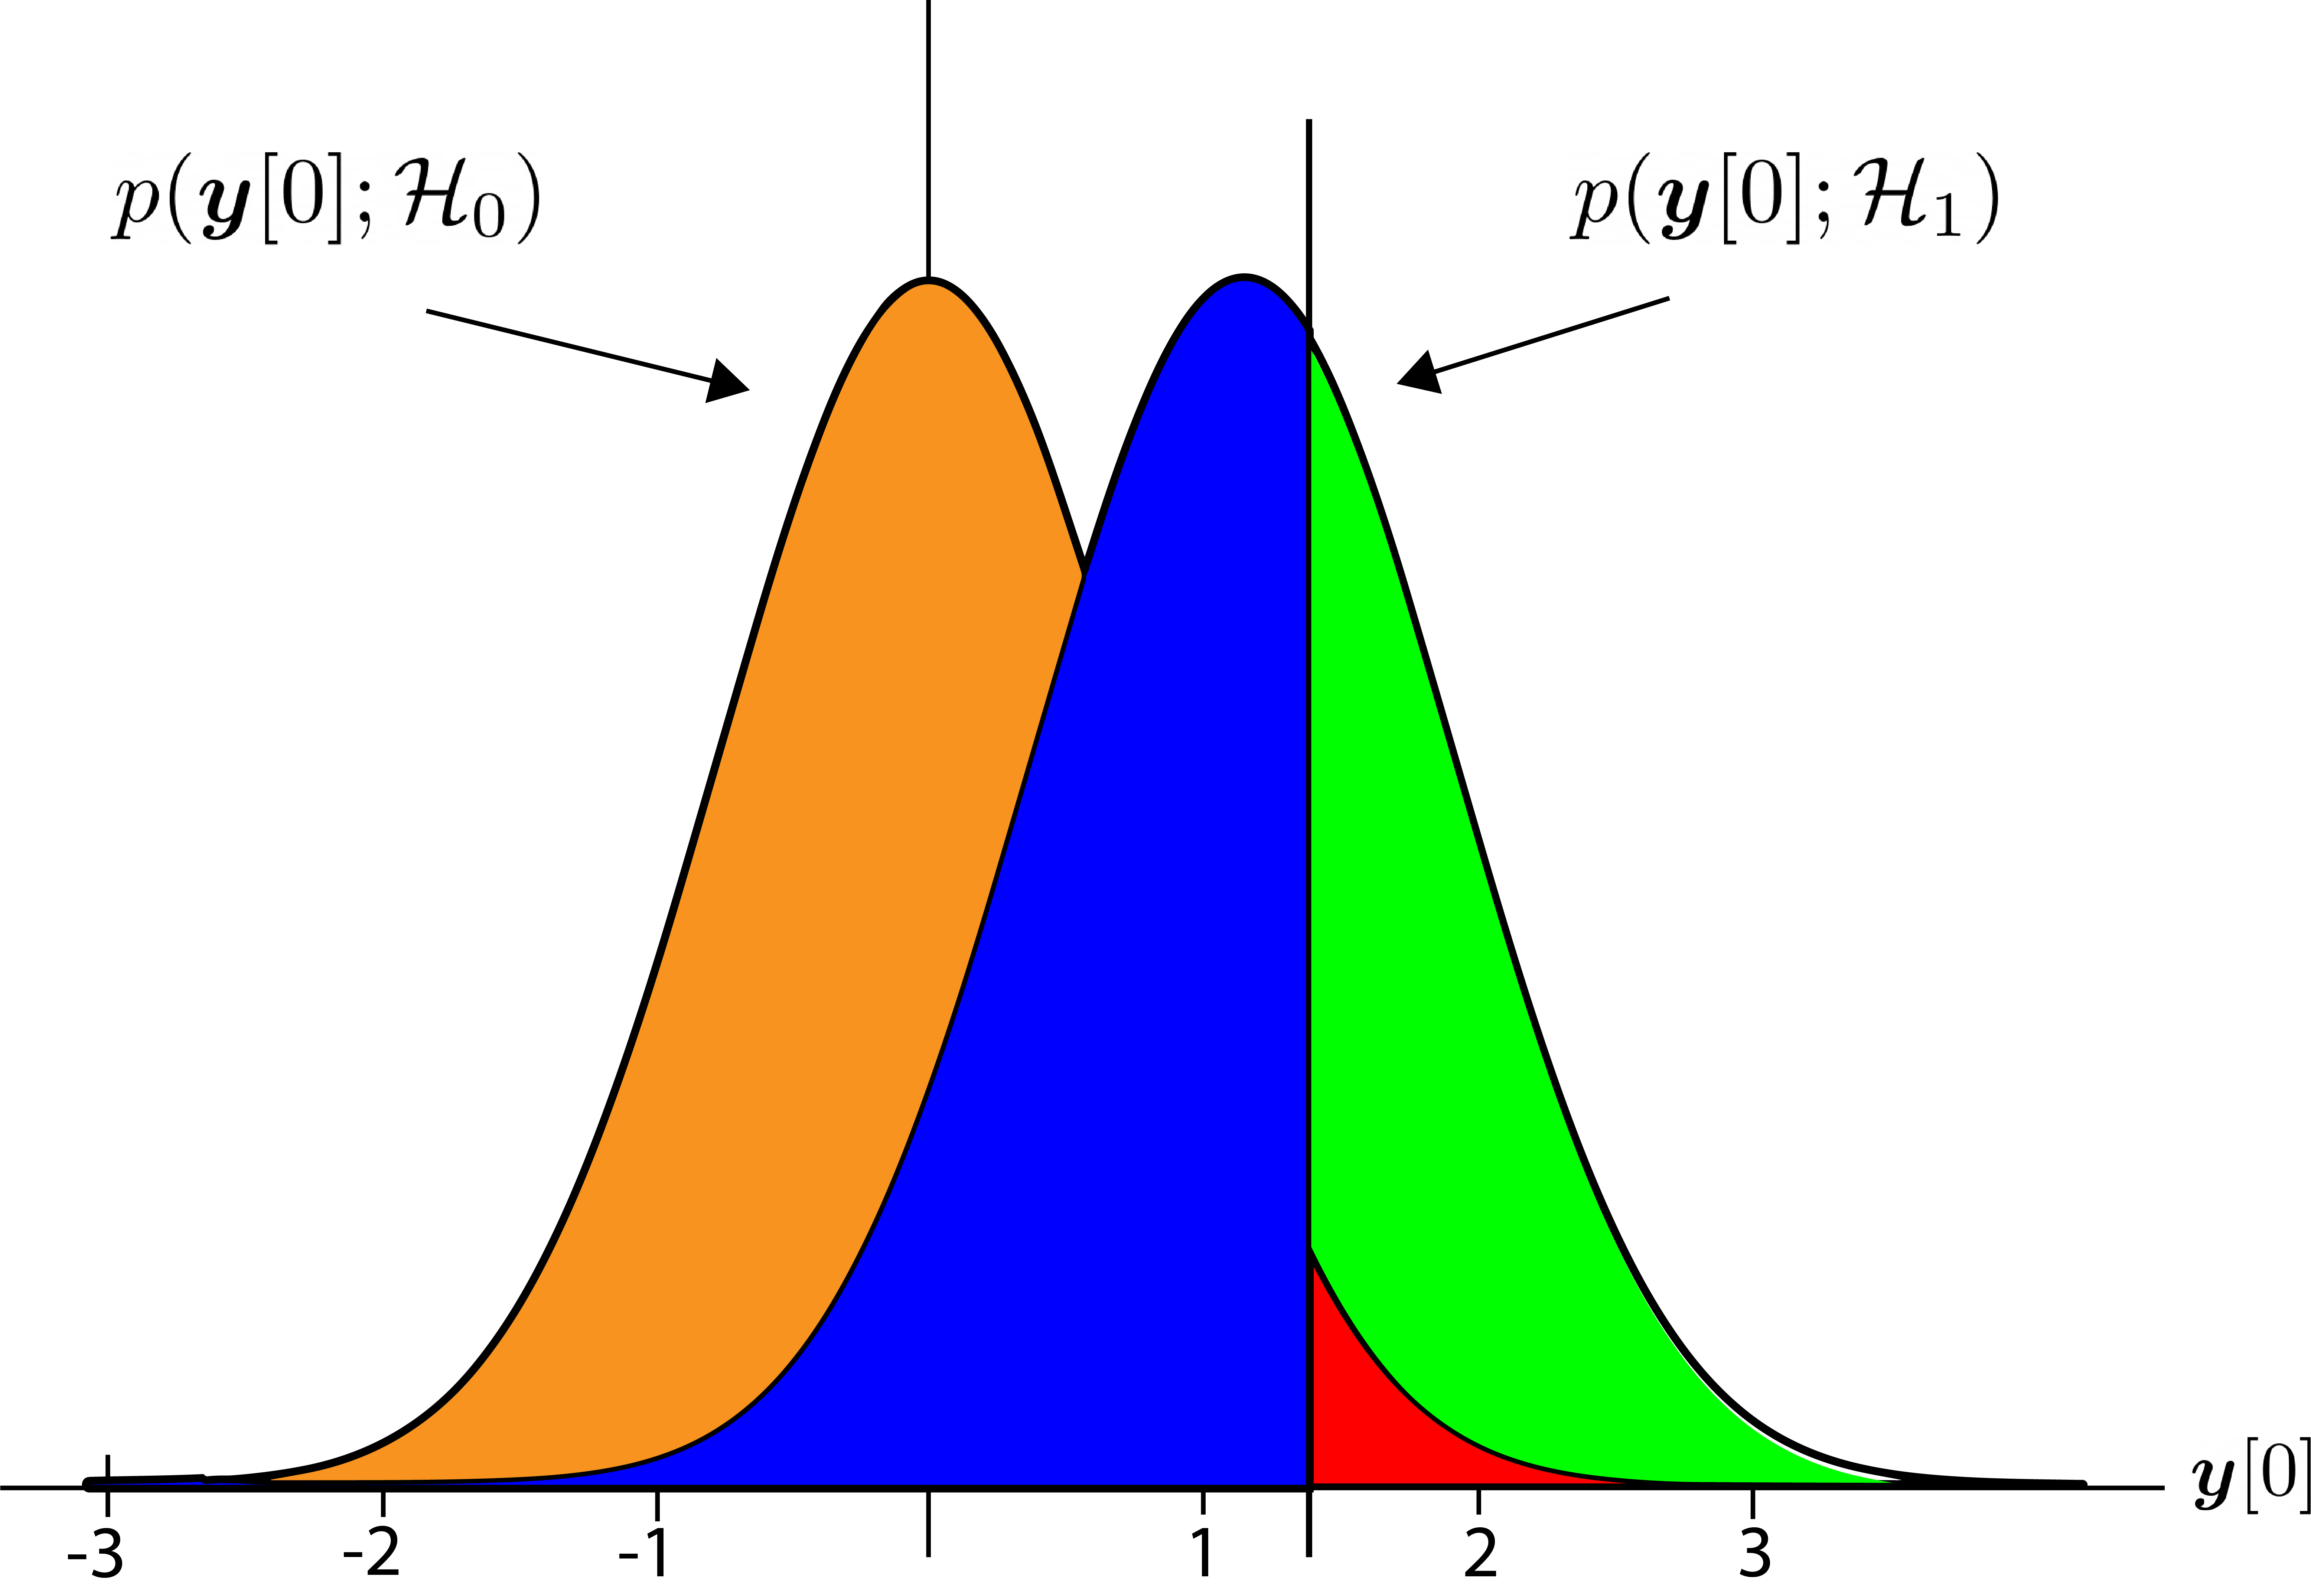
\includegraphics[width=\textwidth]{figs/Chapter-4/230523_detection_theory2.png}
        \caption{}
    \end{subfigure}
    \caption{An illustration of two PDFs associated a binary hypothesis test. The decision threshold is represented by the vertical line that partitions both distributions. The orange and red areas correspond to the true negative and false positive probabilities and the blue and green areas correspond to the false negative and true positive probabilities respectively. To decided between the two hypotheses the likelihood ratio test specified by the Neyman-Pearson theorem is applied. This approach achieves the highest true positive probability for a given false positive probability.}
    \label{fig:chap4-detection-threshold}
\end{figure}
Two types of misclassifications are possible. Either one declares noise data as signal, which is called a false positive, or one declares signal data as noise, which is a false negative. Note that it is only possible to trade off these two types of errors by tuning the detection threshold. One cannot reduce the rate of false positives without also increasing the rate of false negatives.

The approach taken with CRES signals is to fix the rate of false positives by setting a minimum decision threshold value. The rate of false positives that is acceptable at the detection stage depends upon the total rate of background events compatible with the sensitivity goals of the experiment. The ultimate goal of a neutrino mass measurement with 40~meV sensitivity in general has strict requirements on the number of background events, which requires a relatively high detection threshold to achieve. Consequently, the ideal signal detection algorithm is the one that achieves the maximum rate of true positives for a fixed rate of false positives, so that the detection efficiency of the experiment is maximized and potential sources of background are kept to a minimum.

According to the Neyman-Pearson theorem \cite{neyman_pearson_lemma}, the statistical hypothesis test that maximizes the probability of detection for a fixed rate of false positives is the likelihood ratio test, which is formed by computing the ratio of the signal likelihood to the noise likelihood,
\begin{equation}
    L(x)=\frac{P(\bm{y};\mathcal{H}_1)}{P(\bm{y};\mathcal{H}_0)}>\gamma.
\end{equation}
Here, the likelihood of the hypotheses $\mathcal{H}_0$ and $\mathcal{H}_1$ are described by the probability distributions $P(\bm{y};\mathcal{H}_0)$ and $P(\bm{y};\mathcal{H}_1)$ respectively, and $\gamma$ is the threshold for deciding $\mathcal{H}_1$. The decision threshold is determined by integrating $P(\bm{y};\mathcal{H}_0)$ such that 
\begin{equation}
    P_{\textrm{FP}}=\int_\gamma^\infty{P(\tilde{\bm{y}};\mathcal{H}_0)d\tilde{\bm{y}}}=\alpha,
\end{equation}
where $\alpha$ is the desired false positive detection rate given by the red colored areas shown in Figure \ref{fig:chap4-detection-threshold}. The true positive detection rate is given by the similar integral 
\begin{equation}
    P_{\textrm{TP}}=\int_\gamma^\infty{P(\tilde{\bm{y}};\mathcal{H}_1)d\tilde{\bm{y}}},
\end{equation}
which corresponds to the green areas in Figure \ref{fig:chap4-detection-threshold}.

Changing the decision threshold allows one to trade-off between $P_{\textrm{TP}}$ and $P_{\textrm{FP}}$ as appropriate for the given situation. It is standard to summarize the relationship between $P_{\textrm{TP}}$ and $P_{\textrm{FP}}$ using the receiver operating characteristic (ROC) curve, which is obtained by evaluating the true positive and false positive probabilities as a function of the decision threshold value (see Figure \ref{fig:chap4-example-roc-curve}).
\begin{figure}[htbp]
    \centering
    \includegraphics*[width=0.7\textwidth]{figs/Chapter-4/230603_roc_curve_example.png}
    \caption{\label{fig:chap4-example-roc-curve} An example ROC curve formed by computing the $P_\mathrm{FP}$ and the $P_\mathrm{TP}$ for a given likelihood ratio test. As the decision threshold is increased $P_\mathrm{FP}$ decreases at the expense of a lower $P_\mathrm{TP}$. The black dashed line indicates the lower bound ROC curve obtained by randomly deciding between $\mathcal{H}_0$ and $\mathcal{H}_1$. }
\end{figure}
The ROC curve provides a convenient way to compare the performance of different signal detection algorithms. In general, a classifier with a higher the $P_\mathrm{TP}$ as a function of $P_\mathrm{FP}$ is desirable, which corresponds to a larger area underneath the respective ROC curve. A perfect classifier has an area underneath the curve of 1.0, however, such a classifier is never achieved in practice. 

\subsection{Digital Beamforming}
\label{sec:chap4-dig-bf}

\subsubsection*{Introduction to Beamforming}

Beamforming is an antenna array signal processing technique designed to enhance the radiation of the array in a particular direction and suppress it in other directions \cite{balanis2015antenna}. Beamforming is of interest to Project 8 as a first level of signal reconstruction for the FSCD and other antenna array CRES experiments, which operates at the signal detection stage of reconstruction.% This is because beamforming is designed to combine the outputs of the different antennas in the array into a single signal, that could be analyzed in a similar way as previous CRES experiments to start and provide the basis for the development of new follow-up analysis algorithms.

Beamforming is perfomed using a phased summation of the signals received by the antenna array. The beamforming phases are selected such that the signals emitted by the array will constructively interfere at the point of interest (see Figure \ref{fig:chap4-basic-bf}). As a consequence of the principle of reciprocity \cite{reciprocity_theorem}, when the array is operating in receive mode, the signals emitted from a source at the same point will constructively interfere when summed.  
\begin{figure}[htbp]
    \centering
    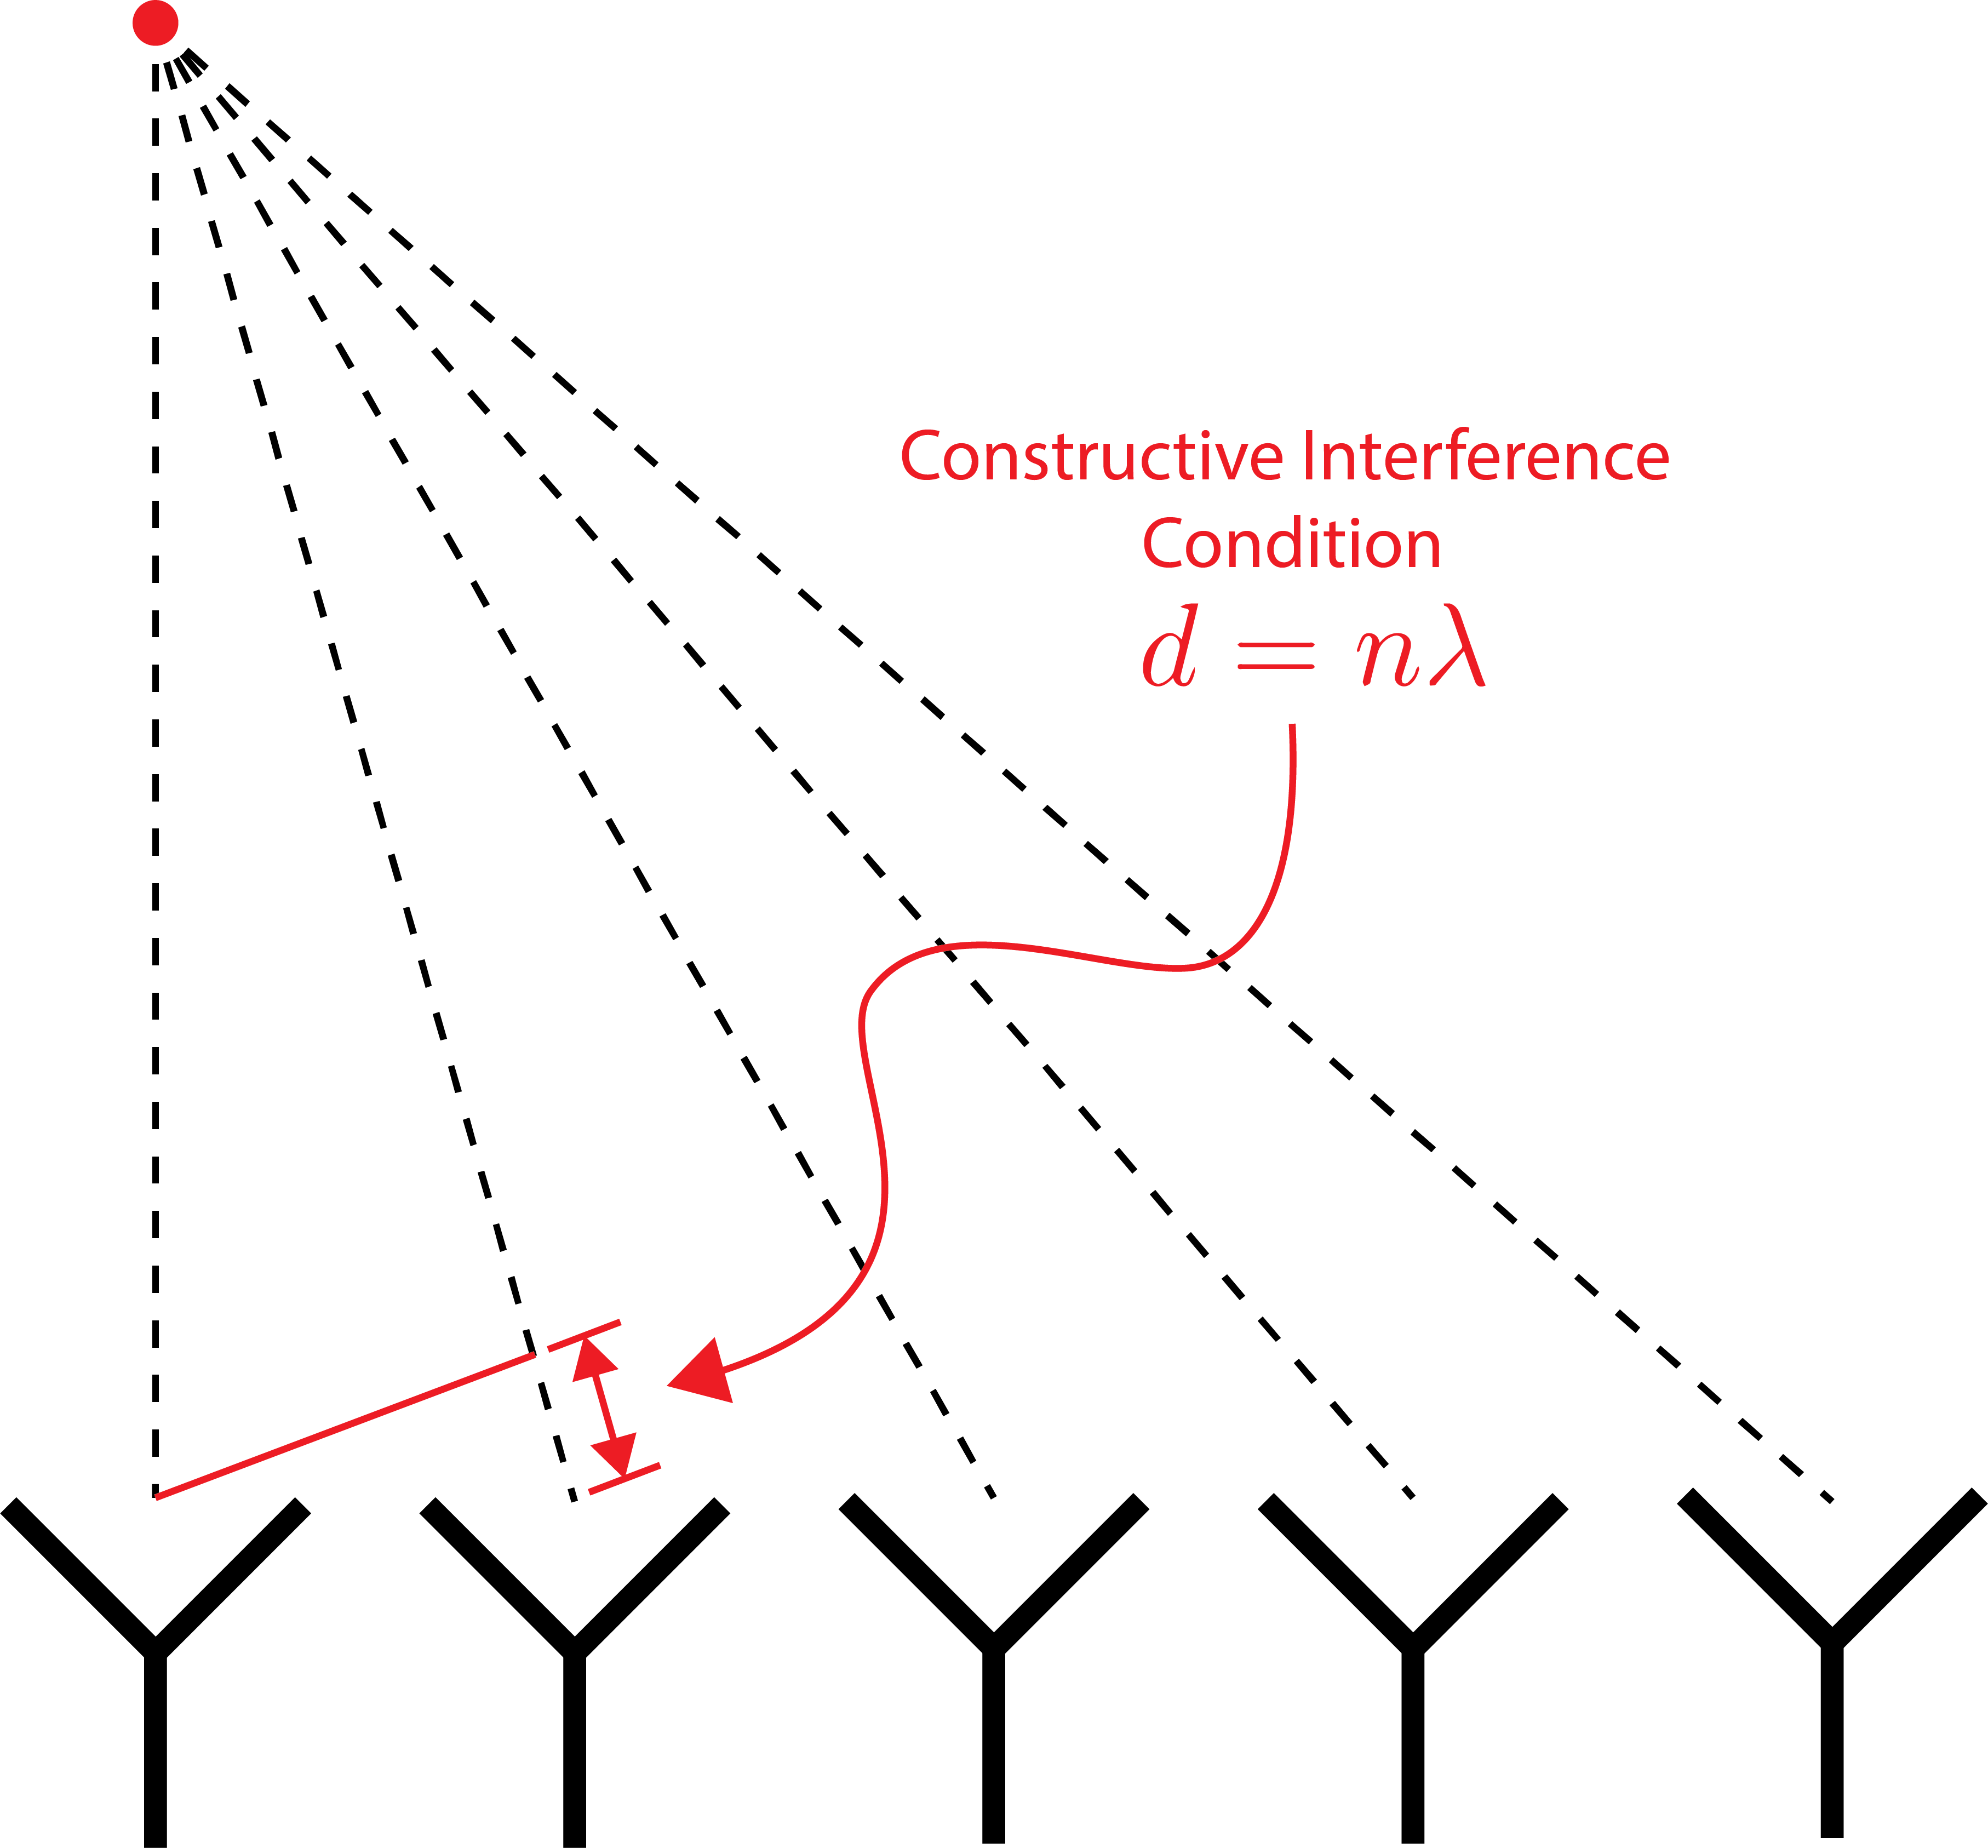
\includegraphics[width=0.6\textwidth]{figs/Chapter-4/230517_basic_bf.png}
    \caption{An illustration of the constructive interference condition which is the operating principle of digital beamforming using a uniform linear array as an example.}
    \label{fig:chap4-basic-bf}
\end{figure}
The origin of the phase delays in beamforming is the path-length difference to the beamforming point between different antennas in the array. The relationship between the phase delay and the path-length difference is given by the familiar equation
\begin{equation}
    \phi=\frac{2\pi d}{\lambda},
    \label{eq:chap4-bf-phases}
\end{equation}
where $\phi$ is the phase delay, $d$ is the path-length difference, and $\lambda$ is the wavelength of the radiation. In practice, one chooses the values of $d$ by specifying the beamforming positions of interest and then calculates the beamforming phases using Equation \ref{eq:chap4-bf-phases}, which is guaranteed to follow the constructive interference condition shown in Figure \ref{fig:chap4-basic-bf}. 

Beamforming can be neatly expressed mathematically using the vector equation
\begin{equation}
    y[n] = \bm{\Phi}^T[n]\bm{x}[n],
\end{equation}
where $\bm{x}[n]$ is the array snapshot vector, $\bm{\Phi}[n]$ is a vector of beamforming shifts, and $y[n]$ is the resulting summed signal. The beamforming shifts consist of a set of complex numbers that contain the beamforming phase shift and an amplitude weighting factor,
\begin{equation}
    \bm{\Phi}[n] = \left[A_0[n]e^{-2\pi i\phi_0[n]}, A_1[n]e^{-2\pi i \phi_1[n]}, ..., A_{N-1}[n]e^{-2\pi i \phi_{N-1}[n]}\right],
\end{equation}
where the set of magnitudes $A_i[n]$ are amplitude weighting factors and $\phi_i[n]$ are the phase shifts from the path-length differences. The index $i$ is used to denote the antenna channel number. The amplitude weighting factor is the relative magnitude of the signal received by a particular antenna in the array. This factor properly accounts for antennas that are closer to the radiating source. In general, the beamforming phases can also be functions of time to track the motion of a non-stationary source.

Digital beamforming specifically is the type of beamforming algorithm of interest to Project 8 for CRES. With digital beamforming, the phase shifts are applied to the array signals in software rather than employing fixed beamforming phase shifts in the receiver chain hardware. The advantage of digital beamforming is that for any given series of array data one can specify an arbitrarily large number of beamforming positions and search for electrons using a flexible and easily configurable beamforming grid.

Digital beamforming can be viewed as the spatial filtering, which is a direct consequence of the constructive interference condition used to define the beamforming phases. Digital beamforming causes signals from multiple electrons at different positions in the trap to be separated, because the interference condition will cause the signals from electrons at other positions to cancel out. This spatial filtering effect reduces pile-up that could become an issue for large scale CRES experiments using a dense tritium source.

Beamforming positions can be specified with arbitrary densities limited only by the available computational resources. This provides a very straight-forward way to estimate the position of the electron in the trap by using a dense grid of beamforming positions and maximizing the output power of the beamforming summation over this grid. This approach to position reconstruction is attractive due the requirements of an event-by-event signal reconstruction, which needs an accurate estimation of the exact magnetic field experienced by the electron in order to correctly estimate its kinetic energy. Combined with an accurate map of the magnetic field inhomogeneities of the trap obtained from calibrations, beamforming allows one to apply this magnetic field correction with a spatial resolution that is a fraction of the cyclotron wavelength.

\subsubsection*{Laboratory Beamforming Demonstrations}

\begin{figure}[htbp]
    \centering
    \includegraphics*[width=0.7\textwidth]{figs/Chapter-4/230725_beamforming_setup_diagram.png}
    \caption{\label{fig:chap4-beamforming-demo-system}A system level diagram of the laboratory setup used for beamforming demonstrations at Penn State. For more information on this system see Chapter 5. Signals near 26~GHz are fed to a dipole antenna using and arbitrary waveform generator (AWG) and vector network analyzer (VNA), which drive a mixer. The dipole radiation is collected by an array of antennas connected to the digitizer data acquisition (DAQ) system.}
\end{figure}

An antenna measurement setup was constructed at Penn State to serve as a testbed for antenna prototypes and to perform laboratory validations of array simulations for the FSCD. This system is discussed in more detail in Chapter 5. Early versions of the antenna measurement system (see Figure \ref{fig:chap4-beamforming-demo-system} and Figure \ref{fig:chap4-beamforming-demo-photos}) were used to perform beamforming reconstruction studies of a simple probe antenna.

\begin{figure}
    \centering
    \includegraphics*[width=0.7\textwidth]{figs/Chapter-4/230725_beamforming_demo_image.png}
    \caption{\label{fig:chap4-beamforming-demo-photos}Photographs of the beamforming demonstration setup. In (a) I show a top-down view of the dipole antenna and the array of eight horn antennas. Manual repositioning of the horn antennas allows one to synthesize a full-circular antenna array. The dipole antenna is mounted on a camera tripod mount that allows for manual position tuning. (b) is a close up image of the dipole, which is manufactured from two segments of semi-rigid coaxial cable. (c) is another image of the dipole and array.}
\end{figure}

Signals from an arbitrary waveform generator were up-converted to 26~GHz using a mixer and a high-frequency source from a vector network analyzer and fed to a dipole antenna through a balun. The radiation from the dipole antenna was received by an array of horn antennas. The signals from the horn antennas were down-converted to baseband using a collection of mixers and an 8-way power divider. The signals were then digitized and saved to a host computer for analysis.

\begin{figure}
    \centering
    \includegraphics*[width=0.85\textwidth]{figs/Chapter-4/230725_beamforming_example.png}
    \caption{\label{fig:chap4-beamforming-demo-example}An example of digital beamforming reconstruction of a dipole antenna using a synthetic array of horn antennas. The beamforming image on the right is constructed by computing the time-averaged power of the summed signals for a two-dimensional grid of beamforming positions. In the image, one can see a clear maximum that corresponds to the position of the dipole antenna. On the left I show the frequency spectrum of the time-series at the maximum power pixel. White Gaussian noise is added to the signal to mimic a more realistic signal-to-noise-ratio. The signal emitted by the dipole is clearly visible as the high power peak in the frequency spectrum.}
\end{figure}

The data collected using the dipole and horn antenna array is reconstructed using the beamforming reconstruction approach specified in Section \ref{sec:chap4-dig-bf}. A two-dimensional grid of xy-positions is defined and the beamforming phase shifts for each of these positions is calculated. The phased summation can be visualized by plotting the time-averaged power for each of the summations as a pixel in the resulting beamforming image (see Figure \ref{fig:chap4-beamforming-demo-example}). White Gaussian noise (WGN) can be added to the data at this stage to simulate more realistic SNR if desired. The beamforming peak maxima is expected to have a Bessel function shape due to the circular symmetry of the array, and by analyzing the size of the beamforming maxima one can confirm that the beamforming reconstruction measurement has similar position resolution as expected from Locust simulations. Additionally, signal detection rates can be estimated from the data by comparing the magnitude of the beamforming signal peak in the frequency spectra to simulation.


\subsubsection*{FSCD Beamforming Simulations}

Locust simulations of the FSCD are used to generate simulated CRES signal data to perform beamforming reconstruction studies. As mentioned in the previous section, the beamforming procedure beings by specifying a set of beamforming positions and corresponding beamforming shifts. The beamforming positions form a grid that covers the region of interest. There are effectively an infinite number of ways to specify the grid positions, however, uniform square grids are the most commonly used due to their simplicity. In the actual experiment the number and pattern of beamforming positions would be optimized to cover the most important regions of the trap volume, which maximizes detection efficiency and minimizes superfluous calculations.

\begin{figure}[htbp]
    \centering
    \begin{subfigure}{0.45\textwidth}
        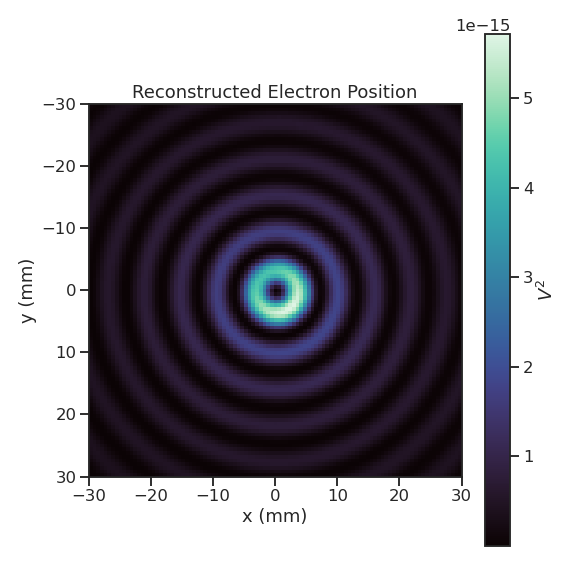
\includegraphics[width=\textwidth]{figs/Chapter-4/230518_locust_bf_onaxis_no_cyclotron.png}
        \caption{\label{fig:chap4-bf-no-cyc-phase-ex}}
    \end{subfigure}
    \hfill
    \begin{subfigure}{0.45\textwidth}
        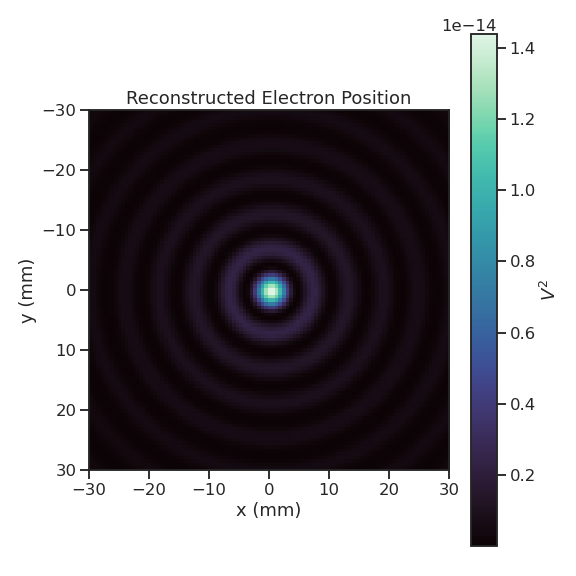
\includegraphics[width=\textwidth]{figs/Chapter-4/230518_locust_bf_onaxis.png}
        \caption{}
    \end{subfigure}
    \caption{Beamforming images visualizing the reconstruction of an electron without (a) and with (b) the cyclotron phase correction. The images were generated using data from Locust simulations. The cyclotron phase refers to a phase offset equal to the relative azimuthal position of an antenna in the array. This phase offset is caused by the circular electron orbit and must be corrected for during reconstruction.}
    \label{fig:chap4-cyclotron-phase-bf-corr}
\end{figure}

The beamforming grids used for signal reconstruction with the FSCD consist of a set of points that cover the two-dimensional plane formed by the perimeter of the antenna array. The axial dimension is left out because electrons are treated as if they occupy only their average axial position, which corresponds to the center of the magnetic trap. This treatment is valid since it is impossible to resolve the axial position of the electron as a function of time due to the rapid oscillation frequencies of trapped electrons.

After beamforming, a summed time-series is obtained for each beamforming position that can be checked for a signal using a detection algorithm. A beamforming image is a visualization method that is equivalent to arranging the beamforming grid points according to their physical locations. Each pixel in the image corresponds to a summed time-series obtained for a digital beamforming position, and the image is obtained taking the time-averaged power at every pixel(see Figure \ref{fig:chap4-cyclotron-phase-bf-corr}).% Beamforming images are purely for the purposes of visualization and are not particularly useful for signal detection or reconstruction.

If only the spatial beamforming phase component from Equation \ref{eq:chap4-bf-phases} is used, then the resulting image contains a ring-shaped feature centered on the position of the electron (see Figure \ref{fig:chap4-bf-no-cyc-phase-ex}). The origin of this shape is an additional phase offset particular to a cyclotron radiation source. The circular cyclotron orbit introduces a relative phase offset to the electric fields equal to the azimuthal position of the field measurement point \cite{nb_thesis, p8synca}. Therefore, two antennas, one located at an azimuthal position of $0^\circ$ and another located at an azimuthal position of $90^\circ$, will receive CRES signals out of phase by $90^\circ$, which is the difference in their azimuthal positions. This phase offset can be corrected by adding an additional term to the beamforming phase equation that is equal to the azimuthal position of the antenna relative to the electron, 
\begin{equation}
    \phi_i[n] = \frac{2\pi d_i[n]}{\lambda} + \Delta\varphi_i[n],
    \label{eq:chap4-beamforming-phases}
\end{equation}
where $\Delta\varphi_i$ is difference between the azimuthal position of the electron and the $i$-th antenna channel. Using the updated beamforming phases changes the ring feature into the expected Bessel peak whose maximum corresponds to the position of the electron. Including this cyclotron phase correction significantly improves the signal detection and reconstruction capabilities of beamforming by more than doubling the summed signal power and shrinking the beamforming maxima feature size. 

The beamforming image examples in Figure \ref{fig:chap4-cyclotron-phase-bf-corr} were produced using an electron located on the central axis of the magnetic trap, which do not experience $\nabla B$-drifts. However, electrons produced at non-zero radial position the beamforming phases must be made time-dependent to track the position of the electron's guiding center over time. Without this correction the $\nabla B$-drift causes the electron to move away from the beamforming position, which effectively spreads the cyclotron radiation power over a wider area in the beamforming image (see Figure \ref{fig:chap4-gradb-bf-drift-corr}).
\begin{figure}[htbp]
    \centering
    \begin{subfigure}{0.45\textwidth}
        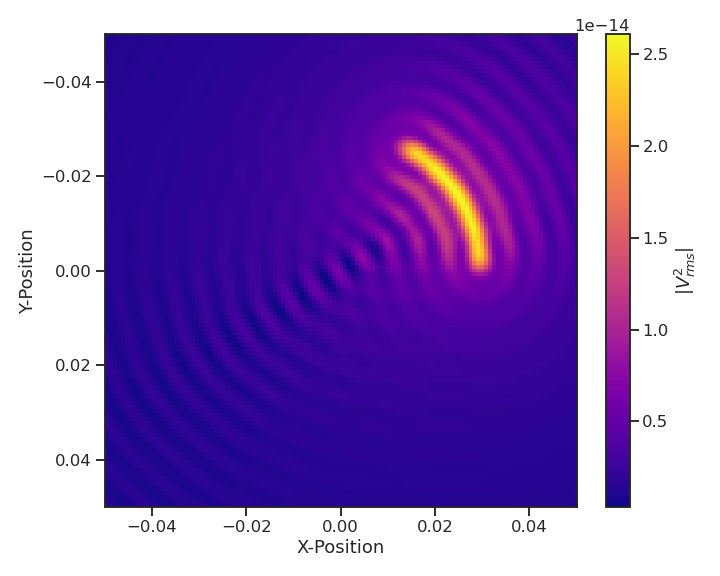
\includegraphics[width=\textwidth]{figs/Chapter-4/220318_88deg_electron_3cm_no_correction.png}
        \caption{}
    \end{subfigure}
    \hfill
    \begin{subfigure}{0.45\textwidth}
        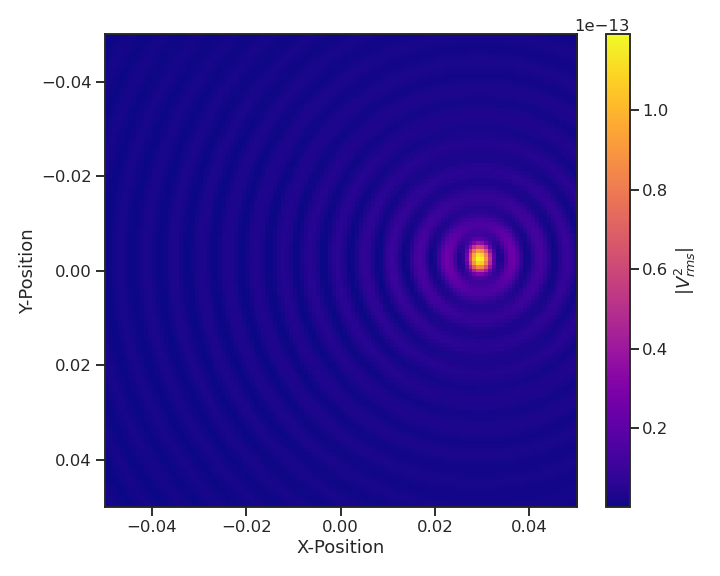
\includegraphics[width=\textwidth]{figs/Chapter-4/220318_88deg_electron_3cm_corrected.png}
        \caption{}
    \end{subfigure}
    \caption{Beamforming images visualizing the reconstruction of an electron located off the central axis of the FSCD trap. In (a) beamforming is being performed without the $\nabla B$-drift correction, and in (b) it is included.}
    \label{fig:chap4-gradb-bf-drift-corr}
\end{figure}
This effect significantly reduces the power of the beamforming maxima and increases the size of the beamforming features, simultaneously harming detection efficiency and position reconstruction. 

The $\nabla B$-drift correction simply adds a circular time-dependence to the beamforming positions as a function of time,
\begin{align}
    r[n]&=r_0\\
    \varphi[n]&=\varphi_0 + \omega_{\nabla B}t[n],
    \label{eq:chap4-grab-b-drift}
\end{align}
where $\omega_{\nabla B}$ is the drift frequency and $t[n]$ is the time vector. In the ideal case the $\nabla B$-drift frequencies from Figure \ref{fig:chap4-gradb-drift-frequency-map} for the correct pitch angle and radial position would be used, however, it is not possible to know the electron's pitch angle a priori. In principle, one could perform multiple beamforming summations for a given beamforming position using different drift frequencies and choose the one that maximizes the summed power, but this approach leads to a huge computational burden that would be impractical for a real FSCD experiment. A compromise is to use an average value of $\omega_{\nabla B}$ obtained by averaging over the drift frequencies for electrons of different pitch angle at a particular radius. This approach keeps the computational cost of time-dependent beamforming to a minimum while still providing a significant increase in the detection efficiency of digital beamforming.

\subsubsection*{Signal Detection with Beamforming and a Power Threshold}

Up to this point I have neglected a specific discussion of how digital beamforming is used for signal detection and reconstruction. Because, strictly speaking, digital beamforming consists only of the phased summation of the array signals and cannot be used alone for signal detection. The example beamforming images shown in Figure \ref{fig:chap4-cyclotron-phase-bf-corr} and Figure \ref{fig:chap4-gradb-bf-drift-corr} were produced using simulated data that contained no noise, which significantly degrades the utility of analyzing the beamforming images for signal detection and reconstruction. 

\begin{figure}[htbp]
    \centering
    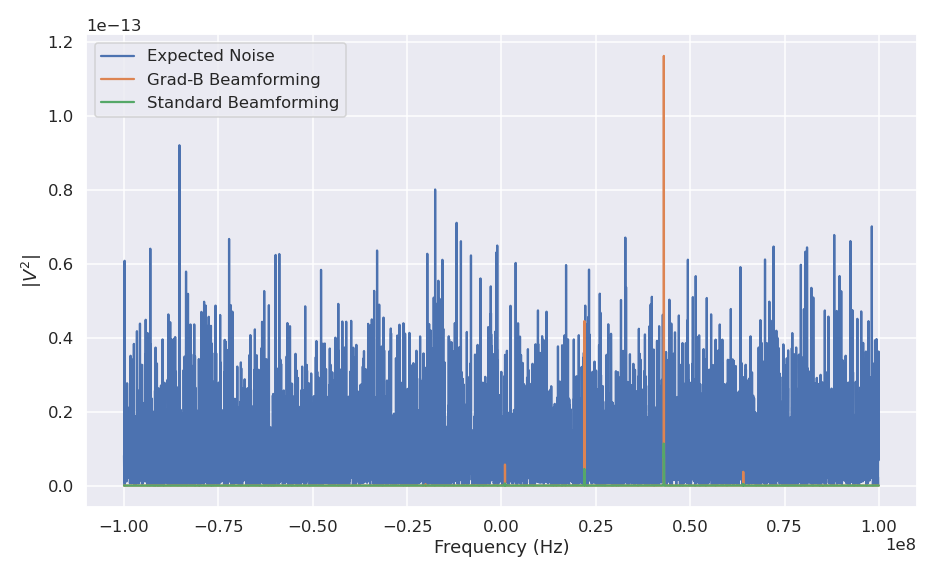
\includegraphics[width=0.67\textwidth]{figs/Chapter-4/220304_example_power_spectrum_gradb_vs_noise_vs_standard_bf.png}
    \caption{A plot of a typical frequency spectrum obtained by applying a Fourier transform to the time-series obtained from beamforming. The frequency spectra are plotted without noise on top of an example of a typical noise spectrum to visualize a realistic signal-to-noise ratio. In the example, without beamforming it would not be possible to detect anything since the signal amplitudes would be reduced by a factor of sixty relative to the noise. Additionally, it is clear the $\nabla B$-drift correction is needed to detect this electron in the prescense of noise.}
    \label{fig:chap4-bf-signal-example}
\end{figure}

In Project 8, digital beamforming as a detection algorithm is understood to mean digital beamforming plus a power or amplitude threshold placed on the frequency spectrum obtained by applying a fast Fourier transform (FFT) to the summed time-series (see Figure \ref{fig:chap4-bf-signal-example}). This approach is similar to the time-frequency spectrogram analysis employed in Phase I and II. However, it is possible to use any signal detection algorithm after beamforming. In Section \ref{sec:chap4-trigger-paper} I analyze the signal detection performance of the power threshold approach in detail.

Without a reconstruction technique that coherently combines the signals from the full antenna, the ability to detect CRES signals is drastically reduced (see Figure \ref{fig:chap4-bf-signal-example}). Because the CRES signals are in-phase at the correct beamforming position, the summed power increases as a function of $N^2$ compared to a single antenna channel, where $N$ is the number of antennas. It is true that the noise power is also increased by beamforming, but, because the noise is incoherent, its power only increases linearly. Consequently, the SNR of the CRES signal increases linearly with the number of antennas, which greatly improves detection efficiency compared to using only the information in a single antenna.

\begin{figure}[htbp]
    \centering
    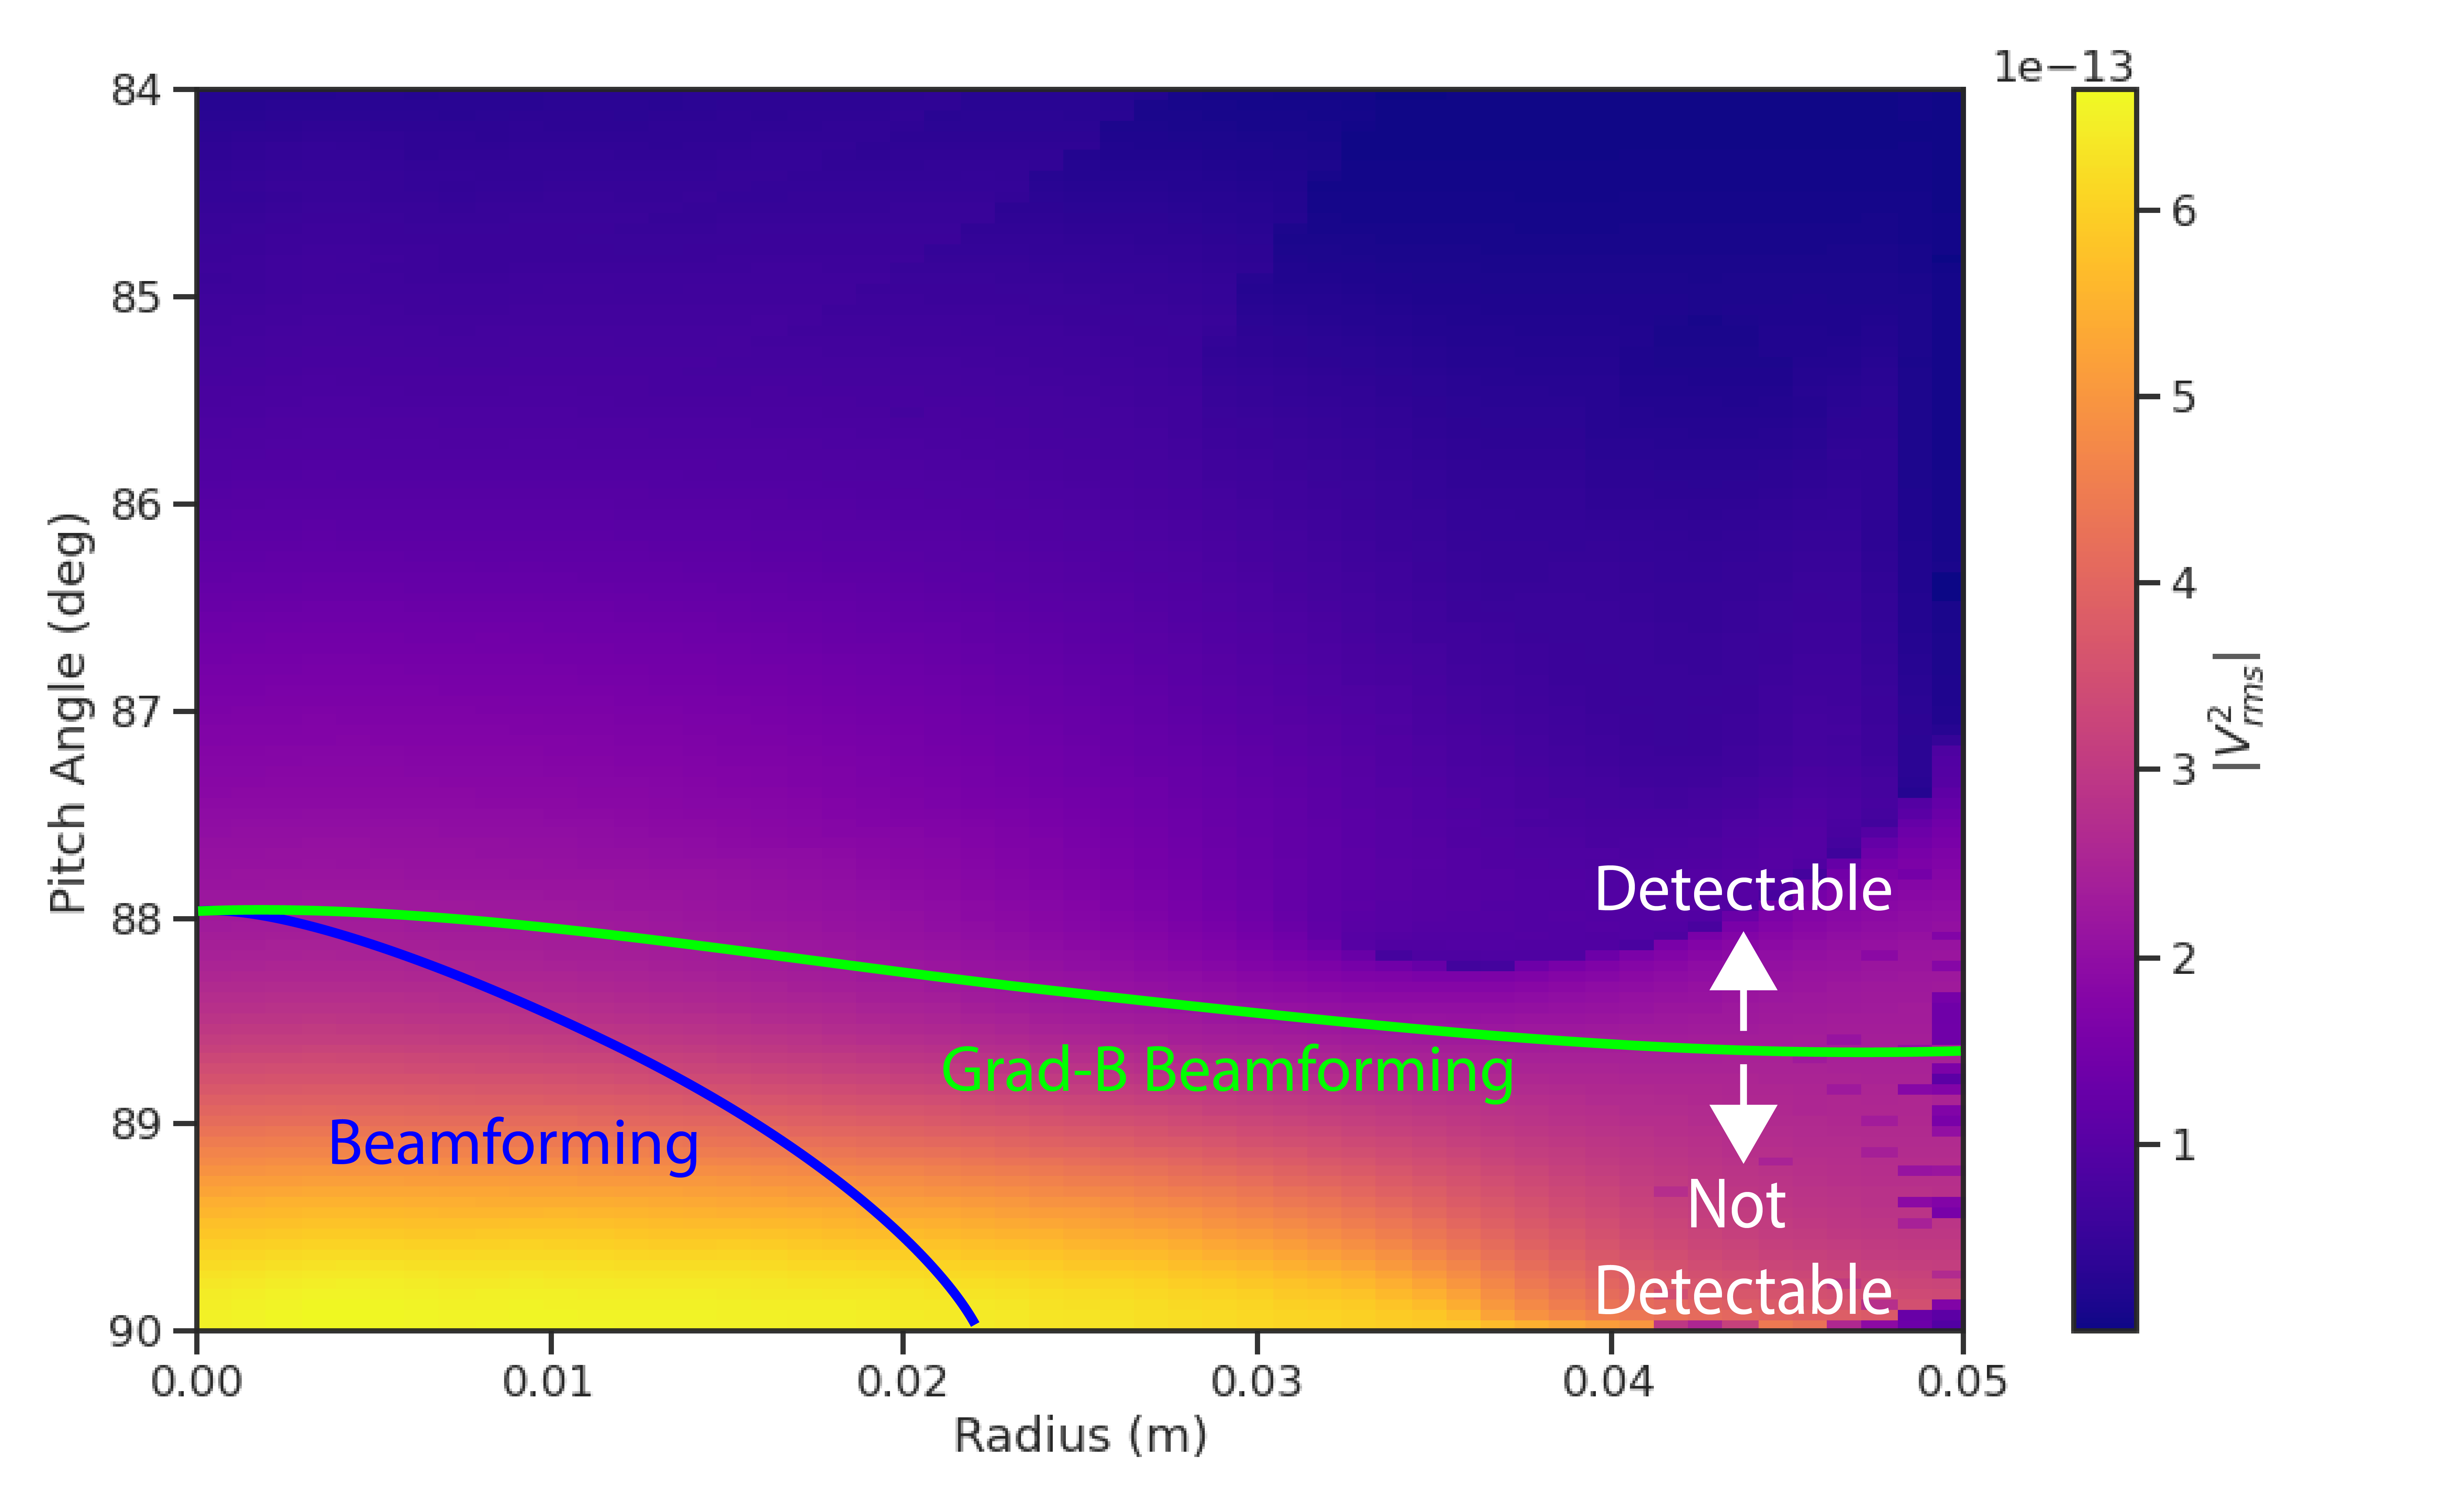
\includegraphics[width=0.67\textwidth]{figs/Chapter-4/230522_beamforming_detectability.png}
    \caption{A plot of the total signal power received by the FSCD array from trapped electrons with different radial positions and pitch angles generated using Locust simulations. The lines on the plot indicate a 10~dB detection threshold above the mean value of the noise in the frequency spectrum. With static beamforming electrons with radial positions larger than about two centimeters are undetectable due to the change in the electron's position over time causing losses from beamforming phase mismatch. This is corrected by including $\nabla B$-drift frequencies in the beamforming phases. Both beamforming techniques fail to detect electrons below $\approx 88.0^\circ$, since these signal are composed of several relatively weak sidebands that are comparable to the noise.}
    \label{fig:chap4-detection-boundaries}
\end{figure}

The power threshold detection algorithm searches for high-power frequency bins that should correspond to a frequency component of the CRES signal. In order to prevent random noise fluctuations from being mistaken as CRES signals the power threshold must be set high enough so that it is unlikely that random noise could be responsible. A consequence of this is that many electrons that can be trapped will go undetected because the modulation caused by axial oscillations leads to the cyclotron carrier power to falling below the decision threshold. The time-dependent beamforming used to correct for the $\nabla B$-drift increases the volume of the magnetic trap where electrons can be detected, but it is ineffective at increasing the range of detectable pitch angles (see Figure \ref{fig:chap4-detection-boundaries}). Fundamentally, this is because the power threshold only uses a fraction of the signal power to detect electrons and ignores the power present in the frequency sidebands. In the subsequent sections I examine two other signal detection algorithms that seek to improve the detection efficiency of the FSCD by utilizing the more of the signal shape to compute the detection test statistics.

\subsection{Matched Filtering}
\label{sec:chap4-matched-filtering-formalism}

\subsubsection*{Introduction to Matched Filtering}

The problem of CRES signal detection is the problem of detecting a signal buried in WGN, which has been examined at great depth in the signal processing literature \cite{detection_theory}. For a fully known signal in WGN the optimal detector is the matched filter, which means that it achieves the highest true positive rate for a fixed rate of false positives.

The matched filter test statistic is calculated by taking the inner product of the data with the matched filter template
\begin{equation}
    \mathcal{T}=\left|\sum_{n}{h^\dagger[n]y[n]}\right|,
    \label{eq:chap4-mf-test-stat-perfect}
\end{equation}
where $h[n]$ is the matched filter template and $y[n]$ is the data. The matched filter test statistic defines a binary hypothesis test in which the data vector is assumed to be an instance of two possible data classes. By setting a decision threshold on the value of $\mathcal{T}$, one can classify a given data vector as belonging to two distinct hypotheses. Under the first hypothesis the data is composed of pure WGN, and under the second hypothesis the data is composed of the known signal with additive WGN.

The matched filter template is obtained by rescaling the known signal in the following way
\begin{equation}
    h[n] = \frac{x[n]}{\sqrt{\tau \sum_{n}{x^\dagger[n]x[n]}}},
    \label{eq:chap4-mf-template-definition}
\end{equation}
where $\tau$ is the variance of the WGN and $x[n]$ is the known signal. Strictly speaking, Equation \ref{eq:chap4-mf-template-definition} is only true for noise with a diagonal covariance matrix, which is assumed to be true for the FSCD. Defining the matched filter templates in this way guarantees that the expectation value of $\mathcal{T}$ is equal to one when the data contains only noise, which is the standard matched filter normalization.

Although matched filters are canonically formulated in terms of a perfectly known signal, it is possible to apply the matched filter technique with imperfect information provided the signal is deterministic. From the discussion of CRES simulation tools (see Section \ref{sec:chap4-simulations}) it was shown that the shape of CRES signals are completely determined by the initial parameters of the electron. The random collisions with background gas molecules, which cause the formation of signal tracks, are the only stochastic component of the CRES event after the initial beta-decay. Therefore, a matched filter can be used for the detection of deterministic CRES signal tracks between scattering events.

\begin{figure}[htbp]
    \centering
    \includegraphics*[width=0.7\textwidth]{figs/Chapter-4/220318_example_convolution.png}
    \caption{Example of a convolution of a CRES signal template with a segment of noisy data. A simulated CRES signal was simulated using Locust and normalized to create a matched filter template. When this template is convolved with noisy data the contains the matching signal the convolution output increases dramatically compared to data with only noise. The decreasing convolution output as the time offset of the convolution increases is caused by zero-padding of the data and template. }
    \label{fig:chap4-mf-convolution-example}
\end{figure}

The matched filter test statistic for CRES signals is a modified version of Equation \ref{eq:chap4-mf-test-stat-perfect}
\begin{equation}
    \mathcal{T} = \max_{\bm{h},m}\left|\bm{h}\ast\bm{y}\right|=\max_{\bm{h},m}\left|\sum_{k}h^\dagger[k]x[m-k]\right|,
    \label{eq:chap4-mf-test-stat-conv}
\end{equation}
where the matched filter inner product has been replaced with a convolution operation and a maximization over the template and convolution delay, $m$ (see Figure \ref{fig:chap4-mf-convolution-example}). Replacing the inner product with a convolution accounts for the fact that the start time of the CRES signal is now an unknown parameter. In addition, a maximization of the matched filter convolution is performed over a number of different templates. Because the shape of the signal is unknown, a range of different signal shapes, called a template bank, must be checked using an exhaustive search.

\subsubsection*{Matched Filtering in the Frequency Domain}

The template bank approach, while powerful, can become computationally intractable. Specifically, the time-domain convolution specified by Equation \ref{eq:chap4-mf-test-stat-conv} is particularly computationally intensive and is a major barrier towards the implementation of a matched filter for signal detection in an experiment like the FSCD. This can be avoided by using the convolution theorem to replace the time-domain convolution with an inner product in the frequency domain. 

The convolution theorem states that 
\begin{equation}
    \bm{f}\ast\bm{g} = \mathcal{F}^{-1}\left(\bm{F}\cdot \bm{G}\right)
    \label{eq:chap4-conv-theorem}
\end{equation}
where $\bm{f}$ and $\bm{g}$ are discretely sampled time-series, $\bm{F}$ and $\bm{G}$ are the respective discrete Fourier transforms, and $\mathcal{F}^{-1}$ is the inverse discrete Fourier transform operator. The convolution theorem allows us to perform the matched filter convolution by first computing the Fourier transform of the template and data, then performing a point-wise multiplication of the two frequency series, and finally performing the inverse Fourier transform to obtain the convolution output. Because discrete Fourier transforms can be performed extremely efficiently, the convolution theorem is almost always used in lieu of directly computing the convolution. 

One thing to note here is that the convolution theorem for discrete sequences shown here, is technically valid only for circular convolutions, which is not directly specified in Equation \ref{eq:chap4-mf-test-stat-conv}. However, because typical CRES track lengths are much longer than the Fourier analysis window and the frequency chirp rates are small compared to the time-slice duration, it is safe to use circular convolutions to evaluate matched filter scores for CRES signals, which allows one to apply the convolution theorem to compute matched filter scores for the FSCD.

\subsubsection*{Matched Filter Analysis of the FSCD}

Since the matched filter is the optimal signal detection approach, it provides the ultimate upper bounds on signal detection. This makes it a useful algorithm for assessing the upper bounds on neutrino mass sensitivity for the FSCD, since it indicates the best possible detection efficiency achievable for that experiment configuration. The standard approach to performing these studies involves generating numerous simulated electron signals that span the kinematic parameter space of electrons.% In general, electrons have six kinematic parameters along with an additional start time parameter. 

To limit the number of simulations required to evaluate the detection efficiency, the standard approach is to fix the starting axial position, starting azimuthal position, starting direction of the perpendicular component of the electron's momentum, and event start time. This reduces the dimensionality of the simulated parameter space to three parameters --- the starting radial position, starting kinetic energy, and starting pitch angle. The fixed variables are nuisance parameters, which do not affect the detection efficiency estimates for the FSCD design, because they simply introduce overall phase offsets that can be marginalized during the calculation of the matched filter score. Across radial position, kinetic energy, and pitch angle one defines a regular grid of parameters and uses Locust to simulate the corresponding signals (see Figure \ref{fig:chap4-mf-parameter-grid}). This grid of simulated signals is used to estimate detection efficiency by calculating the detection probability of a randomly parameterized signal using the grid as a set of matched filter templates (see Section \ref{sec:chap4-trigger-paper}).

\begin{figure}[htbp]
    \centering
    \includegraphics*[width=0.6\textwidth]{figs/Chapter-4/230725_matched_filter_grid_example.png}
    \caption{\label{fig:chap4-mf-parameter-grid} An example two-dimensional parameter distribution of a matched filter template bank and random test signals. $\theta$ refers to the pitch angle of the electron and $E$ is the kinetic energy. The template bank forms a regular grid of in pitch angle and energy; whereas, the test signals are uniformly distributed in pitch angle and follow the tritium beta-decay kinetic energy distribution. This is why there are fewer test signals at higher energies. The need for high match across the full parameter space prevents one from reducing the density of templates in this low activity region. A zoomed in version of the template bank illustrates the relative density of templates and signals needed for match $>90\%$. }
\end{figure}

The matched filter approach can also be used to estimate the achievable energy resolution of the experiment by using a dense grid of templates generated with parameters close to the unknown signal (see figure \ref{fig:chap4-mf-score-dense-grid}). Because matched filter templates with similar parameters have closely matching signal shapes, templates with incorrect parameters can have nearly identical matched filter scores as the correct template. Since only one sample of noise is included in a sample of real data, one cannot guarantee that the template with the maximum score corresponds to the ground truth parameters of the signal. This introduces uncertainty into the signal parameter estimation that manifests as an energy broadening. Dense grids of matched filter templates allow one to quantify this broadening by analyzing the parameter space of templates with matched filter scores close to the ground truth. This approach is analogous to maximum likelihood estimation and is one key component of a complete sensitivity analysis for an antenna array CRES experiment.

\begin{figure}[htbp]
    \centering
    \includegraphics*[width=0.7\textwidth]{figs/Chapter-4/230725_example_mf_score_map.png}
    \caption{\label{fig:chap4-mf-score-dense-grid} The matched filter scores of a dense grid of templates in pitch angle energy space. Dense template grids allow one to estimate the kinetic energy of the electron by identifying the best matching template. The uncertainty on this value is proportional to the space of templates that also match the test signal well. In the worst case matched filter templates can be completely degenerate where templates with different parameters match a signal with equal likelihood. }
\end{figure}

A figure of merit that summarizes the performance of a matched filter template bank at signal detection is "mean match", which is defined as the average ratio of the highest matched filter score for a random signal to the matched filter score for a perfectly matching template. In equation form the match ratio for a single template is given by
\begin{equation}
    \textrm{Match}\equiv\Gamma=\frac{\mathcal{T}_\mathrm{best}}{\mathcal{T}_\textrm{ideal}},
\end{equation}
where $\mathcal{T}_\textrm{best}$ is the matched filter score of the best fitting template in the bank and $\mathcal{T}_\textrm{ideal}$ is the hypothetical score one would measure if the signal perfectly matched the template. The mean match is the average value of match for a typical signal inside the parameter range covered by the matched filter template bank. Generally, one desires a mean match as close to unity as possible, which is typically an exponential function of the number of templates in the template bank (see Figure \ref{fig:chap4-mean-match-dense-grid}).
\begin{figure}[htbp]
    \centering
    \includegraphics*[width=0.7\textwidth]{figs/Chapter-4/220114_mean_match_vs_number_of_templates_87.0_0cm_modify_sample_number.png}
    \caption{\label{fig:chap4-mean-match-dense-grid} The mean match of the dense template grid shown in Figure \ref{fig:chap4-mf-score-dense-grid} for different numbers of templates. Grids of different sizes were obtained by decimating a dense grid of templates and the average match for each grid was computed using the same set of randomly distributed test signals. Plotting the mean match against the size of the grid allows one to visualize the exponential relationship between match and template bank size. The noise in each curve is caused by sampling effects from the decimation algorithm. In general, longer templates are harder to match than shorter templates.}
\end{figure}
%This behavior is observed for dense matched filter grids like the one in Figure \ref{fig:chap4-mf-score-dense-grid}. A dense grid was used to calculate the average value of match for different template bank sizes shown in Figure \ref{fig:chap4-mean-match-dense-grid}. 

The exponential relationship between match and template bank size manifests for dense and sparse template grids. Sparse template grids are used for signal detection when no prior information on the signal is available; whereas, dense templates grids are more useful for parameter estimation. The mean match value directly influences the detection efficiency of the template bank, but due to the exponential scaling, achieving a high average match at the detection stage can easily overwhelm the available computational resources.

\begin{figure}[htbp]
    \centering
    \includegraphics*[width=0.7\textwidth]{figs/Chapter-4/220223_mf_roc_curve_comparison_with_bf.png}
    \caption{\label{fig:chap4-mf-roc-curve-match-analysis} Matched filter template bank ROC curves as a function of mean match. One can see that for low match a matched filter is on average worse than the more straight forward beamforming detection approach. }
\end{figure}

The effect of match on the detection efficiency of the matched filter template bank can be summarized using the ROC curve (see Figure \ref{fig:chap4-mf-roc-curve-match-analysis}). The average performance of the template bank can be described by a single ROC curve obtained by averaging over the PDFs that describe the detection probabilities of each template in the bank. 

The distribution that describes the matched filter score under the signal hypothesis is a Rician distribution, which has a mean value equal to the matched filter score multiplied by the match ratio (see Section \ref{sec:chap4-trigger-paper}). Alternatively, the distribution of the matched filter score when there is no signal in the data follows a Rayleigh distribution, which is equivalent to a Rician distribution with zero mean. The matched filter score for each template in the template bank is described by a separate Rician distribution. Therefore, one way to model detection probability for a given signal is to average across all matched filter distributions in the template bank to obtain a single distribution that describes the statistical behavior of the matched filter score.

%Since a large number of templates are checked for a given piece of data, a statistical trials penalty, which is the statistical penalty one pays for randomly checking many templates in order to avoid a random match between noise and a template, is included by computing the joint distribution of $N_\mathrm{template}$ Rayleigh distributions, where $N_\mathrm{template}$ is the size of the template bank. For more information on the calculation of matched filter template bank ROC curves please refer to Section \ref{sec:chap4-trigger-paper}.

A different way to visualize the detection performance for each algorithm is to specify a minimum acceptable false positive rate at the trigger level. This is equivalent to specifying a minimum threshold on the value of the matched filter score or the size of a frequency peak for a beamforming power threshold trigger. One can then draw regions of detectable signals as a function of the electron's pitch angle and radial position (see Figure \ref{fig:chap4-estimated-detection-threshold-parameter-space}).
\begin{figure}[htbp]
    \centering
    \includegraphics*[width=0.7\textwidth]{figs/Chapter-4/220318_static_vs_bf_vs_mf_vs_dnn_detection_threshold_electron_paramter_map.png}
    \caption{\label{fig:chap4-estimated-detection-threshold-parameter-space} Boundaries of detectable electrons in pitch angle kinetic energy space for a series of different signal detection algorithms. A detectable signal is defined as a signal that is above a consistent decision with at least 50\% probability. This non-rigorous treatment of detection probability is primarily useful for the visualization the relative increases in detection performance provided by the different algorithms. The static beamforming (Static-BF) algorithm is the digital beamforming algorithm introduced above without the $\nabla B$-drift correction. The DNN algorithm refers to a convolutional neural network classifier trained to detect CRES signals (see Section \ref{sec:chap4-intro-ml}). }
\end{figure}
A kinetic energy shift is equivalent to an overall frequency shift of the signal and should have no effect on the detection probability assuming sufficient density of matched filter templates in the energy dimension. A electron is declared "detectable" for the regions in Figure \ref{fig:chap4-estimated-detection-threshold-parameter-space} if the signal has at least 50\% probability of falling above the decision threshold of the respective classifier. One can see that the parameter space of detectable signals is greatly expanded beyond the beamforming power threshold trigger with a matched filter (MF) or deep neural network (DNN) (see Section \ref{sec:chap4-intro-ml}). Plots such as Figure \ref{fig:chap4-estimated-detection-threshold-parameter-space} are useful for visualization, but, since the handling of detection likelihood is not sufficiently rigorous, the detection probability boundaries are not well-suited to sensitivity estimates.

\subsubsection*{Optimized Matched Filtering Implementation for the FSCD}

The biggest practical obstacle to the implementation of a matched filter template bank is the computational cost associated with exhaustively calculating the matched filter scores; therefore, one must employ several optimizations in a practical setting. 

Computing a matched filter score requires the convolution of two vectors, which can be performed very efficiently by computers if the convolution theorem and fast Fourier transforms (FFT) are utilized. Furthermore, one can apply digital beamforming as a pre-processing step to reduce the dimensionality of the data before the matched filter. In order to understand the relative gain in computational efficiency offered by these optimizations I analyze the total number of floating-point operations (FLOP) of several matched filter implementations in big $O$ notation that utilize different combinations of optimizations. 

A direct implementation of a matched filter as specified by Equation \ref{eq:chap4-mf-test-stat-conv} involves the convolution of $N_\mathrm{ch}$ signals of length $N_\mathrm{s}$ with template signals of length $N_\mathrm{t}$. The FLOPs of the various matched filter implementations on a per-template basis will be used as a consistent metric, since each implementation scales linearly with the number of templates. The direct convolution approach to matched filtering costs
\begin{equation}
    O(N_\mathrm{ch})\times O(N_\mathrm{s}\times N_\mathrm{t})
\end{equation}
FLOP per-template, whose cost is dominated by the $O(M\times N)$ convolution operation. 

The computational cost of the direct matched filter approach can be significantly reduced by exploiting the convolution theorem and FFT algorithms. By restricting oneself to signals and templates that contain equal numbers of samples, the convolution can be calculated by Fourier transforming both vectors, performing the point-wise multiplication, and taking the inverse Fourier transform to obtain the convolution result. The FFT algorithm is able to compute the Fourier transform utilizing only $O(N\log{N})$ operations. This optimization results in a computational cost per-template of
\begin{equation}
    O(N_\mathrm{ch})\times O(N_\mathrm{s}\log{N_\mathrm{s}})
\end{equation}
A typical signal vector in the FSCD contains $O(10^4)$ samples in which case the FFT reduces the computational cost of the matched filter by a factor of $O(10^3)$. In practice, due to the large reduction in computational cost with a frequency-domain matched filter, direct implementations of the matched filter using a time-domain convolution are almost never attempted in practice. Particularly, a time-domain matched filter is completely computationally infeasible for the FSCD due to resource constraints.

Rather than relying solely on the matched filter it is tempting to consider using digital beamforming as an initial step in the signal reconstruction for the purposes of data reduction. The primary motivation is to reduce the dimensionality of the data by a factor of $N_\mathrm{ch}$ by combining the array outputs coherently into a single channel. One can view the beamforming operation as a partial matched filter, in the sense that the matched filter convolution contains the beamforming phased summation along with a prediction of the signal shape. By separating beamforming from the signal shape one hopes to reduce the overall computational cost by effectively shrinking the number of templates and reducing the number of operations required to check each one.

The nature of this optimization requires that one account for the number of templates used for pure matched filtering versus the hybrid approach. To first order, the total number of templates at the trigger stage is a product of the number of guesses for each of the electron's parameters
\begin{equation}
    N_\mathrm{T}=N_\mathrm{E}\times N_\theta \times N_\mathrm{r} \times N_\mathrm{\varphi},
\end{equation}
where $N_\mathrm{E}$ is the number of kinetic energies, $N_\theta$ is the number of pitch angles, $N_\mathrm{r}$ is the number of starting radial positions, and $N_\mathrm{\varphi}$ is the number of starting azimuthal positions. The starting axial position and cyclotron motion phase are not necessary to include in the template bank, since these parameters manifest themselves as the starting phase of the signal, which is effectively marginalized when using a FFT to compute the matched filter convolution. Therefore, the total number of operations required by a matched filter to detect a signal in a segment of array data is on the order of 
\begin{equation}
    O(N_\mathrm{T})\times O(N_\mathrm{ch})\times O(N_\mathrm{s}\log{N_\mathrm{s}})
    \label{eq:chap4-tot-ops-pure-mf}
\end{equation}

With the hybrid approach one removes spatial parameters from the template bank by using beamforming to combine the array signals into a single channel. Beamforming explicitly assumes a starting position, which allows one to use matched filter templates that span the two-dimensional space of kinetic energy and pitch angle. The total computational cost of the hybrid method is directly proportional to the number of beamforming positions. For the time-dependent beamforming defined in Section \ref{sec:chap4-dig-bf}, the number of beamforming positions is given by 
\begin{equation}
    N_\mathrm{BF}=N_\mathrm{r}\times N_\mathrm{\varphi}\times N_\mathrm{\omega_{\nabla B}},
\end{equation}
where $N_\mathrm{r}$ and $N_\mathrm{\varphi}$ are the same spatial parameters encountered in the pure matched filter template bank and $N_\mathrm{\omega_{\nabla B}}$ is the number of $\nabla B$-drift frequency assumptions. If a unique drift frequency is used for each pitch angle then the hybrid approach is effectively equivalent to a pure matched filter in the number of operations. The key efficiency gain of the hybrid approach is to exploit the relatively small differences in $\omega_{\nabla B}$ for electrons of different pitch angles by using only a few average drift frequencies. 

The total number of operations for the hybrid approach can be expressed as a sum of the operations required by the beamforming and matched filtering steps,
\begin{equation}
    O(N_\mathrm{BF})\times O(N_\mathrm{ch}N_\mathrm{s}) + O(N_\mathrm{BF})\times O(N_\mathrm{E}N_\mathrm{\theta})\times O(N_\mathrm{s}\log{N_\mathrm{s}}).
    \label{eq:chap4-tot-ops-bf-hybrid}
\end{equation}
The first product in the sum is the number of operations required by beamforming, which is simply the number of beamforming points times the computational cost of the beamforming matrix multiplication, and the second product is the computational cost of matched filtering the summed signal generated by each beamforming position. To compare this to pure matched filtering, one takes the ratio of Equations \ref{eq:chap4-tot-ops-pure-mf} and \ref{eq:chap4-tot-ops-bf-hybrid} to obtain 
\begin{equation}
    \Gamma_\mathrm{BFMF}=\frac{O(N_{\omega_{\nabla B}})}{O(N_\mathrm{E}N_\mathrm{\theta})\times O(\log{N_\mathrm{s}})} + \frac{O(N_{\omega_{\nabla B}})}{O(N_\mathrm{ch})}.
\end{equation}
This expression can be simplified by observing that $O(N_\mathrm{E}N_\theta)\times O(\log{N_\mathrm{s}})\gg O(N_\mathrm{ch})$, which means that the ratio of computational cost for the two methods can be reduced to
\begin{equation}
    \Gamma_\mathrm{BFMF}\approx \frac{O(N_{\omega_{\nabla B}})}{O(N_\mathrm{ch})}.
\end{equation} 
Limiting onself to a number of estimated drift frequencies of $O(1)$, then it can be seen that the estimated computational cost reduction of the hybrid approach is of $O(N_\mathrm{ch})$. This is a large reduction considering that the FSCD antenna array contains sixty antennas in the baseline design. 

The main drawback of the hybrid approach is that the limited number of allowed drift frequency guesses can lead to detection efficiency loss due to phase mismatch. The degree of phase error from an incorrect drift frequency is proportional to the length of the array data vector used by the signal detection algorithm. For signals with lengths equal to the baseline FSCD Fourier analysis window of 8192 samples, typical phase errors from using an average versus the exact $\nabla B$-drift frequency are on the order of a few percent in terms of the signal energy. This has a relatively small impact on the overall detection efficiency, however, future experiments with antenna array CRES will want to balance optimizations such as these during the design phase to keep experiment costs to a minimum while still achieving scientific goals.

\subsubsection*{Kinetic Energy and Pitch Angle Degeneracy}

Accurate modeling of a matched filter requires one to consider the effects of mismatched signals and template, since this more accurately reflects the real-world usage of a matched filter. One way to study this is to use a signal grid to compute the matched filter scores between mismatched signals and templates and evaluate the matched filter scores under this scenario. What one finds when performing this analysis is that templates for signals with incorrect parameters can have matched filter scores that are indistinguishable from the matched filter score of the correct template (see Figure~\ref{fig:chap4-mf-degeneracy} and Figure~\ref{fig:chap4-mf-degeneracy-large-scale}).
\begin{figure}[htbp]
    \centering
    \begin{subfigure}{0.49\textwidth}
        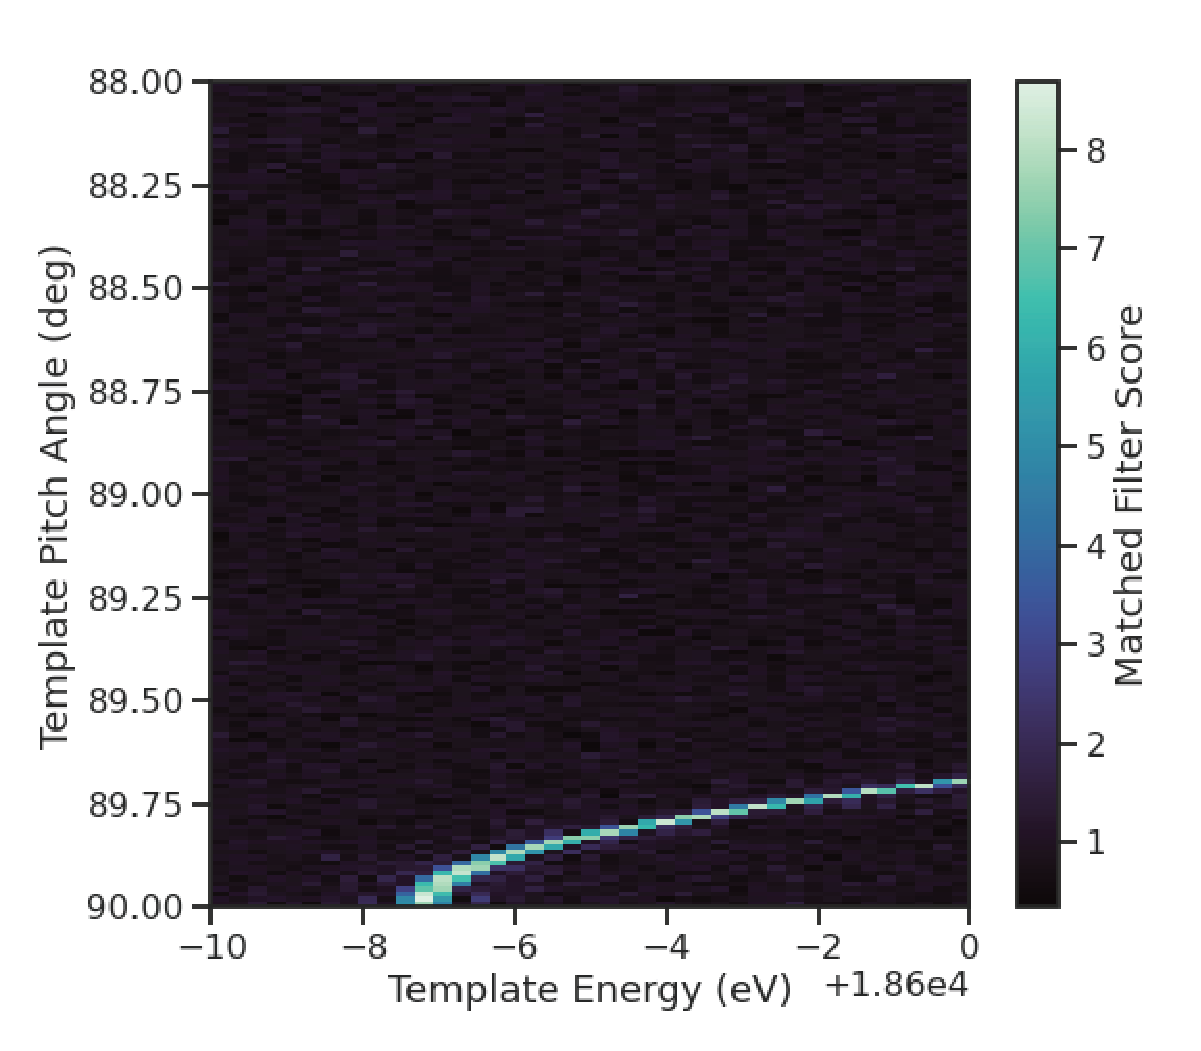
\includegraphics[width=\textwidth]{figs/Chapter-4/230517_mf_degen_1.png}
        \caption{}
    \end{subfigure}
    \hfill
    \begin{subfigure}{0.49\textwidth}
        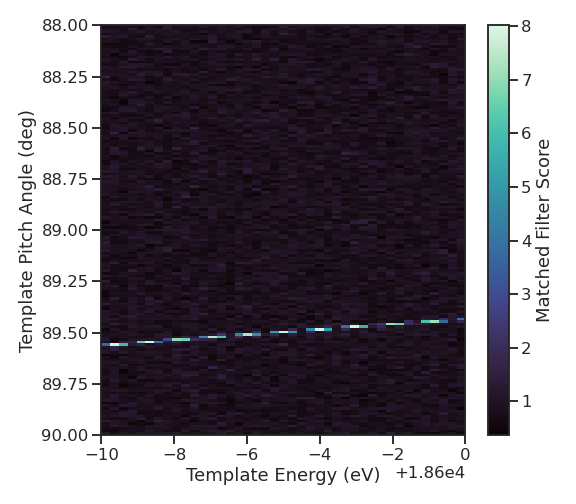
\includegraphics[width=\textwidth]{figs/Chapter-4/230517_mf_degen_2.png}
        \caption{}
    \end{subfigure}
    \caption{Two example illustrations of the correlation between kinetic energy and pitch angle imparted by the shape of the FSCD magnetic trap. The correlations manifest themselves as degeneracies in the matched filter score where multiple matched filter templates have the same matched filter for a particular signal. These degeneracies are a sign that the magnetic trap must be redesigned in order to break the correlation between pitch angle and kinetic energy. }
    \label{fig:chap4-mf-degeneracy}
\end{figure}

This degeneracy in matched filter score is the result of correlations between the kinetic energy and pitch angle of the electron caused by the magnetic trap. These correlations are unacceptable since they greatly reduce the energy resolution of the experiment by causing electrons with specific kinetic energy to match templates across a wide range of energies.
\begin{figure}[htbp]
    \centering
    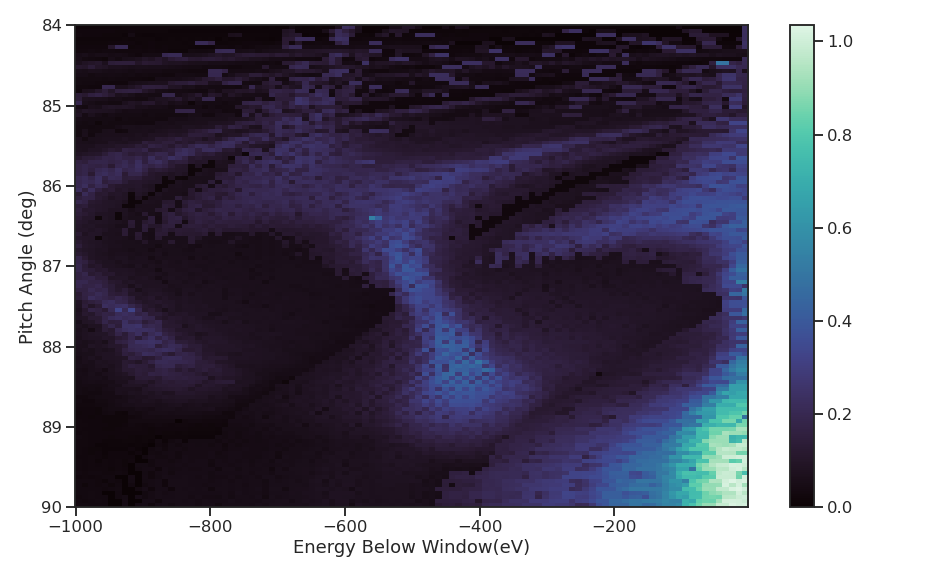
\includegraphics[width=0.7\textwidth]{figs/Chapter-4/230517_energy_pitch_correlation_map.png}
    \caption{A visualization of the correlation between energy and pitch angle in the FSCD magnetic trap. The image is formed by computing the match of the best template from a grid consisting of pitch angles from 84 to 90 degrees in steps of 0.05 degrees, kinetic energies from 17574 to 18574 eV, located at 2~cm from the central axis, and simulated for a length of three FSCD time-slices. The signals used to compute the best matching template consisted of a grid from 84 to 90 degrees in steps of 0.05 degrees, kinetic energies from 18550 to 18575 eV in steps of 0.25 eV, located 2~cm from the central axis, and simulated for three FSCD time-slices. The colored regions of the plot show how well signals with lower energy can match those of higher energy for the FSCD magnetic trap, which is proportional to the achievable energy resolution of the FSCD design.}
    \label{fig:chap4-mf-degeneracy-large-scale}
\end{figure}

This degeneracy cannot be fixed by implementing a different signal reconstruction algorithm. As revealed by the matched filter scores the shapes of the signals for different parameters are identical. Resolving this degeneracy between pitch angle and energy requires the design of a new magnetic trap with steeper walls so that the average magnetic field experienced by an electron is less dependent on pitch angle.

\subsection{Machine Learning}

Machine learning is a broad field of research \cite{prml} that has been particularly transformative in the recent past. In this Section I provide a brief introduction to some concepts and techniques of machine learning that were applied to CRES signal detection in my dissertation.

\subsubsection*{Introduction to Machine Learning}
\label{sec:chap4-intro-ml}

Digitization of the FSCD antenna array generates large amounts of data that must be rapidly processed for real-time signal detection and reconstruction. While digital beamforming combined with a power threshold is relatively computationally inexpensive, it is ineffective at detecting CRES signal with small pitch angles, since it relies on a visible frequency peak above the noise. On the other hand, a matched filter is able to detect signals with a significantly larger range of parameters, however, the exhaustive search of matched filter templates can be computationally expensive. Machine learning based triggering algorithms have been used successfully in many high-energy physics experiments \cite{ml_lhc}, and recently have shown success in the detection of gravitational wave signals \cite{ml_ligo_1,ml_ligo_2} in place of more traditional matched filtering methods. The success of machine learning in these domains motivates the exploration of machine learning as a potential CRES signal detection algorithm. 

Various approaches to machine learning are possible, but the one most important to the discussion here is the supervised learning approach. In supervised learning, one uses a differentiable model or function that is designed to map the input data to the appropriate label \cite{prml}. The data is represented as a multidimensional matrix of floating point values such as an image or a time-series, and the label is typically a class name such as signal or noise for classification problems, or a continuous value like kinetic energy for regression problems. 

In supervised learning the model is trained to map from the data to the correct label by evaluating the output of the model using a training dataset consisting of a set of paired data and labels. To evaluate the difference between the model output and the correct label a loss function is used to quantify the error between the model prediction and the ground truth. For example, a common loss function in regression problems is the squared error loss function, which quantifies error using the squared difference between the model output and label. 

Using the outputs of the loss function the next step in supervised learning is to compute the gradient of error with respect to the model parameters in a process called backpropagation. The gradients are used to update the model parameter values in order to minimize errors in the model predictions across the whole dataset. This loop is performed many times while randomly shuffling the dataset until the error converges to a minimum value at which point the training procedure has finished. It is standard practice to monitor the training procedure by evaluating the performance of the model using a separate validation dataset that matches the statistical distribution of the training data and to check the performance of the model after training using yet another dataset called the test dataset. These practices help to guard against overtraining which is a concern for models with many parameters.

\subsubsection*{Convolutional Neural Networks}

A popular class of machine learning models are neural networks. A neural network is a function composed of a series of linear operations called layers, which take a piece of data typically represented as a matrix, multiply the elements of the data by a weight, and then sums these products to produce an output matrix. Neural networks composed of purely linear operations are unable to model complex non-linear behavior. Therefore, non-linear activation functions are applied to the outputs of each of the layers to increase the ability of the neural network to model complex relationships between the data. 

Neural networks are typically composed of at least three layers, but with the present capabilities of computer hardware they typically contain much more than this. The first layer in a neural network is called the input layer, because it takes the data objects as input, and the last layer in a neural network is known as the output layer. The output layer is trained by machine learning to map the data to an output label using the supervised learning procedure described in Section~\ref{sec:chap4-intro-ml}. Between the input and the output layers are typically several hidden layers that receive inputs from and transmit outputs to other layers in the neural network model. The term deep neural network (DNN) refers to those neural networks that have at least one hidden layer, which have proven to be extremely powerful tools for pattern recognition and function approximation.

An important type of DNN are convolutional neural networks (CNN) that typically contain several layers which perform a convolution of the input with a set of filters. These convolution operations are typically accompanied by layers that attempt to down-sample the data along with the standard neural network activation functions. A standard CNN is composed of several convolutional layers at the beginning of the network and ends with a series of fully-connected neural network layers at the output. Intuitively, one can imagine that the convolutional layers are extracting features from the data that fully-connected layers use to perform the classification or regression task.

\subsubsection*{Deep Filtering for Signal Detection in the FSCD}

\begin{figure}[htbp]
    \centering
    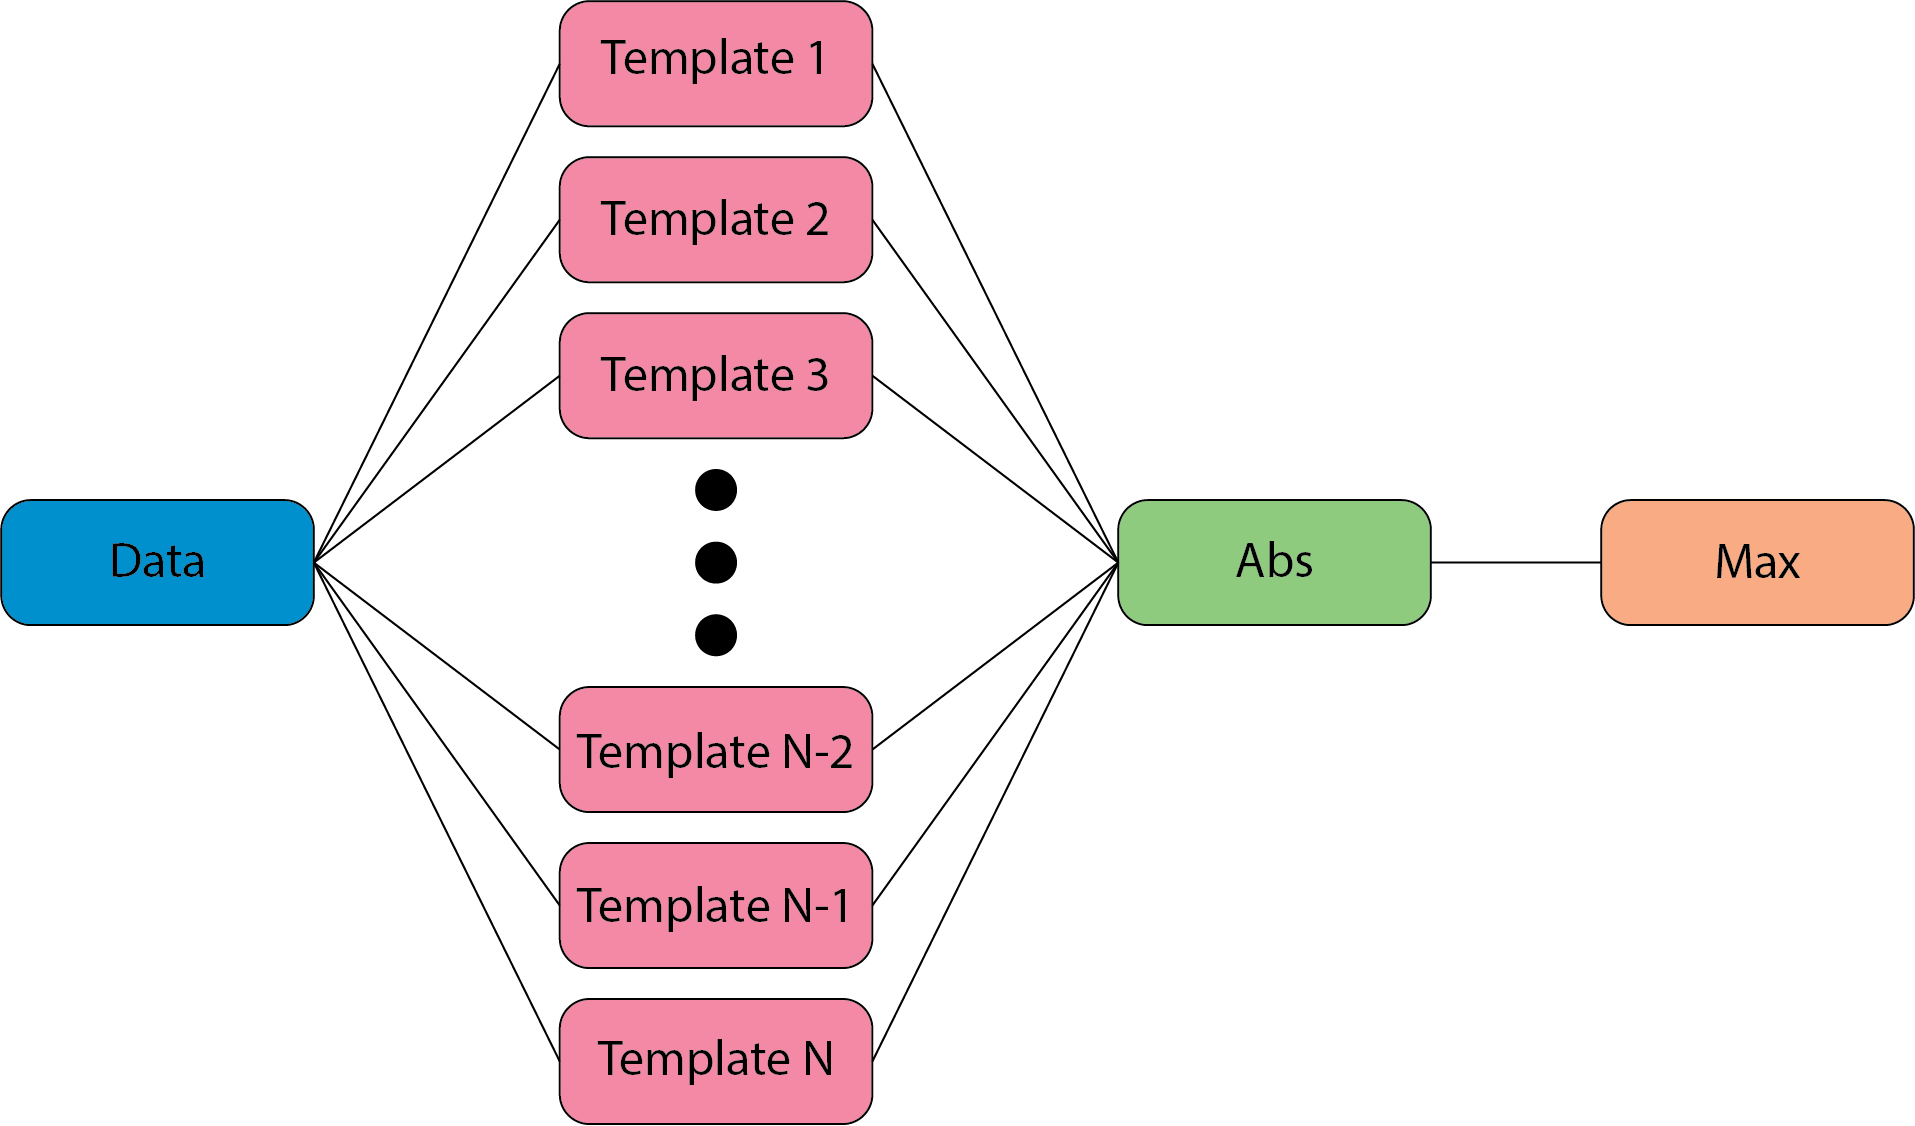
\includegraphics[width=0.66\textwidth]{figs/Chapter-4/230517_mf_conv_net.png}
    \caption{A representation of a matched filter template bank as a convolutional neural network. The network has a single layer composed of the templates, which act as convolutional filters. The activation of the neural network is an absolute value followed by a max operator.}
    \label{fig:chap4-mf-neural-network}
\end{figure}

CNNs have been extremely influential in the field of computer vision, particularly tasks such as image segmentation and classification, but have also been applied in numerous experimental physics contexts. Given the particular challenge posed by signal detection and reconstruction in the FSCD, CNNs are an interesting choice for real-time signal detection, since this application requires both high efficiency and fast evaluation.

In the machine learning paradigm, signal detection is a binary classification problem between the signal and noise data classes. My investigation focuses specifically on the application of CNNs to signal detection in the FSCD, which is motivated by relatively recent demonstrations of CNNs achieving classification accuracies for gravitational wave time-series signals comparable to a matched filter template bank. In this framework it is possible to interpret the matched filter as a type of CNN composed of a single convolutional layer with the templates making up the layer filters (see Figure \ref{fig:chap4-mf-neural-network}). Since this neural network has no hidden layers, it is not a DNN, but one can attempt to construct a proper CNN that attempts to reproduce the classification performance of the matched filter network, which can be refered to as "deep filtering".

The reason why deep filtering can be effective is that it may be possible to exploit redundancies and correlations between templates, which allows one to perform signal detection with similar accuracy but with fewer computations.This is relevant to real-time detection scenarios like the FSCD experiment. In Section \ref{sec:chap4-trigger-paper} I perform a detailed comparison of the signal detection performance of a CNN to beamforming and a matched filter template bank.

Deep filtering is conceptually a simple technique. Similar to a matched filter template bank, many simulated CRES signals are generated and used to train a model to distinguish between signal and noise data (see Figure \ref{fig:chap4-deepfilter-process}). To reduce the dimensionality of the input FSCD data, a digital beamforming summation is applied to the raw time-series data generated by Locust to compress the 60-channel data to a single time-series. CRES signals have a sparse frequency representation and experiments training CNN's on time-series and frequency-series data found that models trained on frequency spectrum data performed significantly better. Therefore, an FFT is applied to the summed time-series before being normalized and fed to the classification model.

\begin{figure}[htbp]
    \centering
    \includegraphics*[width=0.9\textwidth]{figs/Chapter-4/230727_deep_filter_process.png}
    \caption{\label{fig:chap4-deepfilter-process} A graphical depiction of CRES signal detection using a CNN. A noisy segment of data is converted to a frequency series using digital beamforming and a FFT. The complex-valued frequency series is input into a trained CNN model that classifies the data as signal or noise using a decision threshold on the CNN output. }
\end{figure}

The data used to train the model consists of an equal proportion of signal and noise frequency spectra. Unique samples of WGN are generated and added to the signals during training time to avoid having to pre-generate and store large samples of noise data. The binary cross-entropy loss function combined with the ADAM optimizer proved effective at training the models to classify CRES data. A simple hyperparameter optimization was performed by manually tuning model, loss function, and optimizer parameters. The model and training loops was implemented in python using the PyTorch deep learning framework. Standard machine learning practices were followed when training the models, such as overtraining monitoring using a validation dataset. Models were trained until the training loss and accuracy converged and then evaluated using a separate test data set.

\begin{figure}[htbp]
    \centering
    \includegraphics*[width=1.0\textwidth]{figs/Chapter-4/210625_plot_dfcnn_efficiency_vs_noise_temp.png}
    \caption{\label{fig:chap4-dfcnn-efficiency} The detection efficiency and false alarm rate (false positive rate) as a function of the decision threshold for different values of the noise temperature. The model is trained to output a value close to one for data that contains a signal and outputs a value near zero when the data contains only noise. One sees that a lower decision threshold will have a high detection efficiency at the cost of a high rate of false alarms. }
\end{figure}

The classification results of the test dataset are used to quantify the relationship between the true positive rate and the false positive rate for the model. The true positive rate is analogous to detection efficiency and the false positive rate is a potential source of background in the detector. One can limit the rate of false positives using a sufficiently high threshold on the model output at the cost of a lower detection efficiency (see Figure \ref{fig:chap4-dfcnn-efficiency} and Figure \ref{fig:chap4-dfcnn-roc}). As expected, the performance of the model at signal classification is negatively effected the noise power, which is quantified by the noise temperature.

\begin{figure}[htbp]
    \centering
    \includegraphics*[width=1.0\textwidth]{figs/Chapter-4/210625_plot_dfcnn_roc_vs_noise_temp.png}
    \caption{\label{fig:chap4-dfcnn-roc}ROC curves for a CNN model classifying CRES signals. One can see that the area under the curve, which is a figure of merit that describes the performance of the classifier, is roughly linearly dependent with the noise temperature.}
\end{figure}


\section{Analysis of Signal Detection Algorithms for the FSCD}
\label{sec:chap4-trigger-paper}
This section consists of a modified manuscript for an antenna-based CRES signal detection paper prepared for publication in JINST. The contents of this paper were still undergoing collaboration review at the time of writing. In it I present a detailed analysis of the signal detection performance of the three signal detection approaches discussed so far using a population of simulated CRES signals generated with Locust. The focus of the paper is on the performance of the signal detection algorithms for pitch angles below $88.5^\circ$ where the beamforming power threshold is least effective. 

\subsection{Introduction}

\label{sec:intro}
%Cyclotron Radiation Emission Spectroscopy (CRES) is a technique for measuring the kinetic energies of charged particles by observing the frequency of the cyclotron radiation that is emitted as they travel through a magnetic field \cite{p8originalcres, p8prl2015}. The Project 8 Collaboration is developing the CRES technique as a next-generation approach to tritium beta-decay endpoint spectroscopy for neutrino mass measurement. Recently, Project 8 has performed the first CRES-based measurement of the tritium beta-decay energy spectrum and neutrino mass \cite{p8prl2023, p8prc2023}.

%Previous CRES measurements have utilized relatively small volumes of radiation source gas that are directly integrated with a waveguide transmission line, which propagates the cyclotron radiation emitted by magnetically trapped electrons to a cryogenic amplifier. While this technology has had demonstrable success, it is not a feasible option for scaling up to larger measurement volumes. In particular, the goal of the Project 8 Collaboration is to use CRES combined with atomic tritium to measure the neutrino mass with a 40~meV sensitivity. Achieving this sensitivity goal will require a multi-cubic-meter scale measurement volume to obtain the required event statistics in the tritium beta-spectrum endpoint region; hence, there is a need for new techniques to enable large volume CRES measurements for future experiments.

One approach is to use antennas to collect a portion of the cyclotron radiation emitted by trapped electrons \cite{p8snowmass2022, p8jphysg}. A promising design is an inward-facing uniform circular array that surrounds a cylindrical containment volume. Increasing the size of the antenna array by adding additional rings of antennas along the longitudinal axis, allows one to grow the experiment volume until a sufficient amount of tritium gas can be observed by the array. A challenging aspect of this approach is that the total radiated power emitted by an electron near the tritium spectrum endpoint is on the order of 1~fW or less in a 1~T magnetic field. Because the CRES signal power and information is spread across the antenna array, detecting the presence of a CRES signal and determining the electron's kinetic energy requires reconstructing the entire array output over the duration of the event, posing a significant data acquisition and signal reconstruction challenge.

Previous measurements with the CRES technique have utilized a threshold on the frequency spectrum formed from a segment of time-series data. This algorithm relies on the detection of a frequency peak above the thermal noise background, which limits the kinematic parameter space of electrons available for reconstruction (see Section \ref{sec:bf-and-stft}). Although a trigger based on the amplitude of the frequency spectrum was adequate for previous Project 8 experiments, this approach does not provide sufficient detection efficiency for future CRES-based measurements of the neutrino mass. Better efficiency is possible by taking advantage of the deterministic CRES signal structure with a matched filter or machine learning based classifier \cite{p8ml_1}. In order to evaluate the relative gains in efficiency that come from utilizing these algorithms for antennas, analytical models that describe the detection performance of a power threshold and matched filter classifier are developed. In addition, a basic convolutional neural network (CNN) is implemented and tested as a first step towards the development of neural-network based classifiers for antenna array based CRES measurements. These results allow for a comparison between the estimated detection efficiencies of each of these methods, which are weighed against the associated computational costs for real-time applications.

The outline of the remainder of this chapter is as follows. Section \ref{sec:real-time-triggering} is an overview of a prototype antenna array CRES experiment, and describes the approach to real-time signal identification. Section \ref{sec:classifiers} develops models for the power threshold and matched filter algorithms and introduces the machine learning approach and CNN architecture. Section \ref{sec:method} describes the process for generating simulated CRES signal data and the details of training the CNN. Finally, Section \ref{sec:results} compares the signal classification accuracy for the three approaches and discusses the relevant trade-offs in terms of detection efficiency and computational cost.

\begin{figure}[h]
    \centering
    \begin{subfigure}{0.48\textwidth}
        \centering
        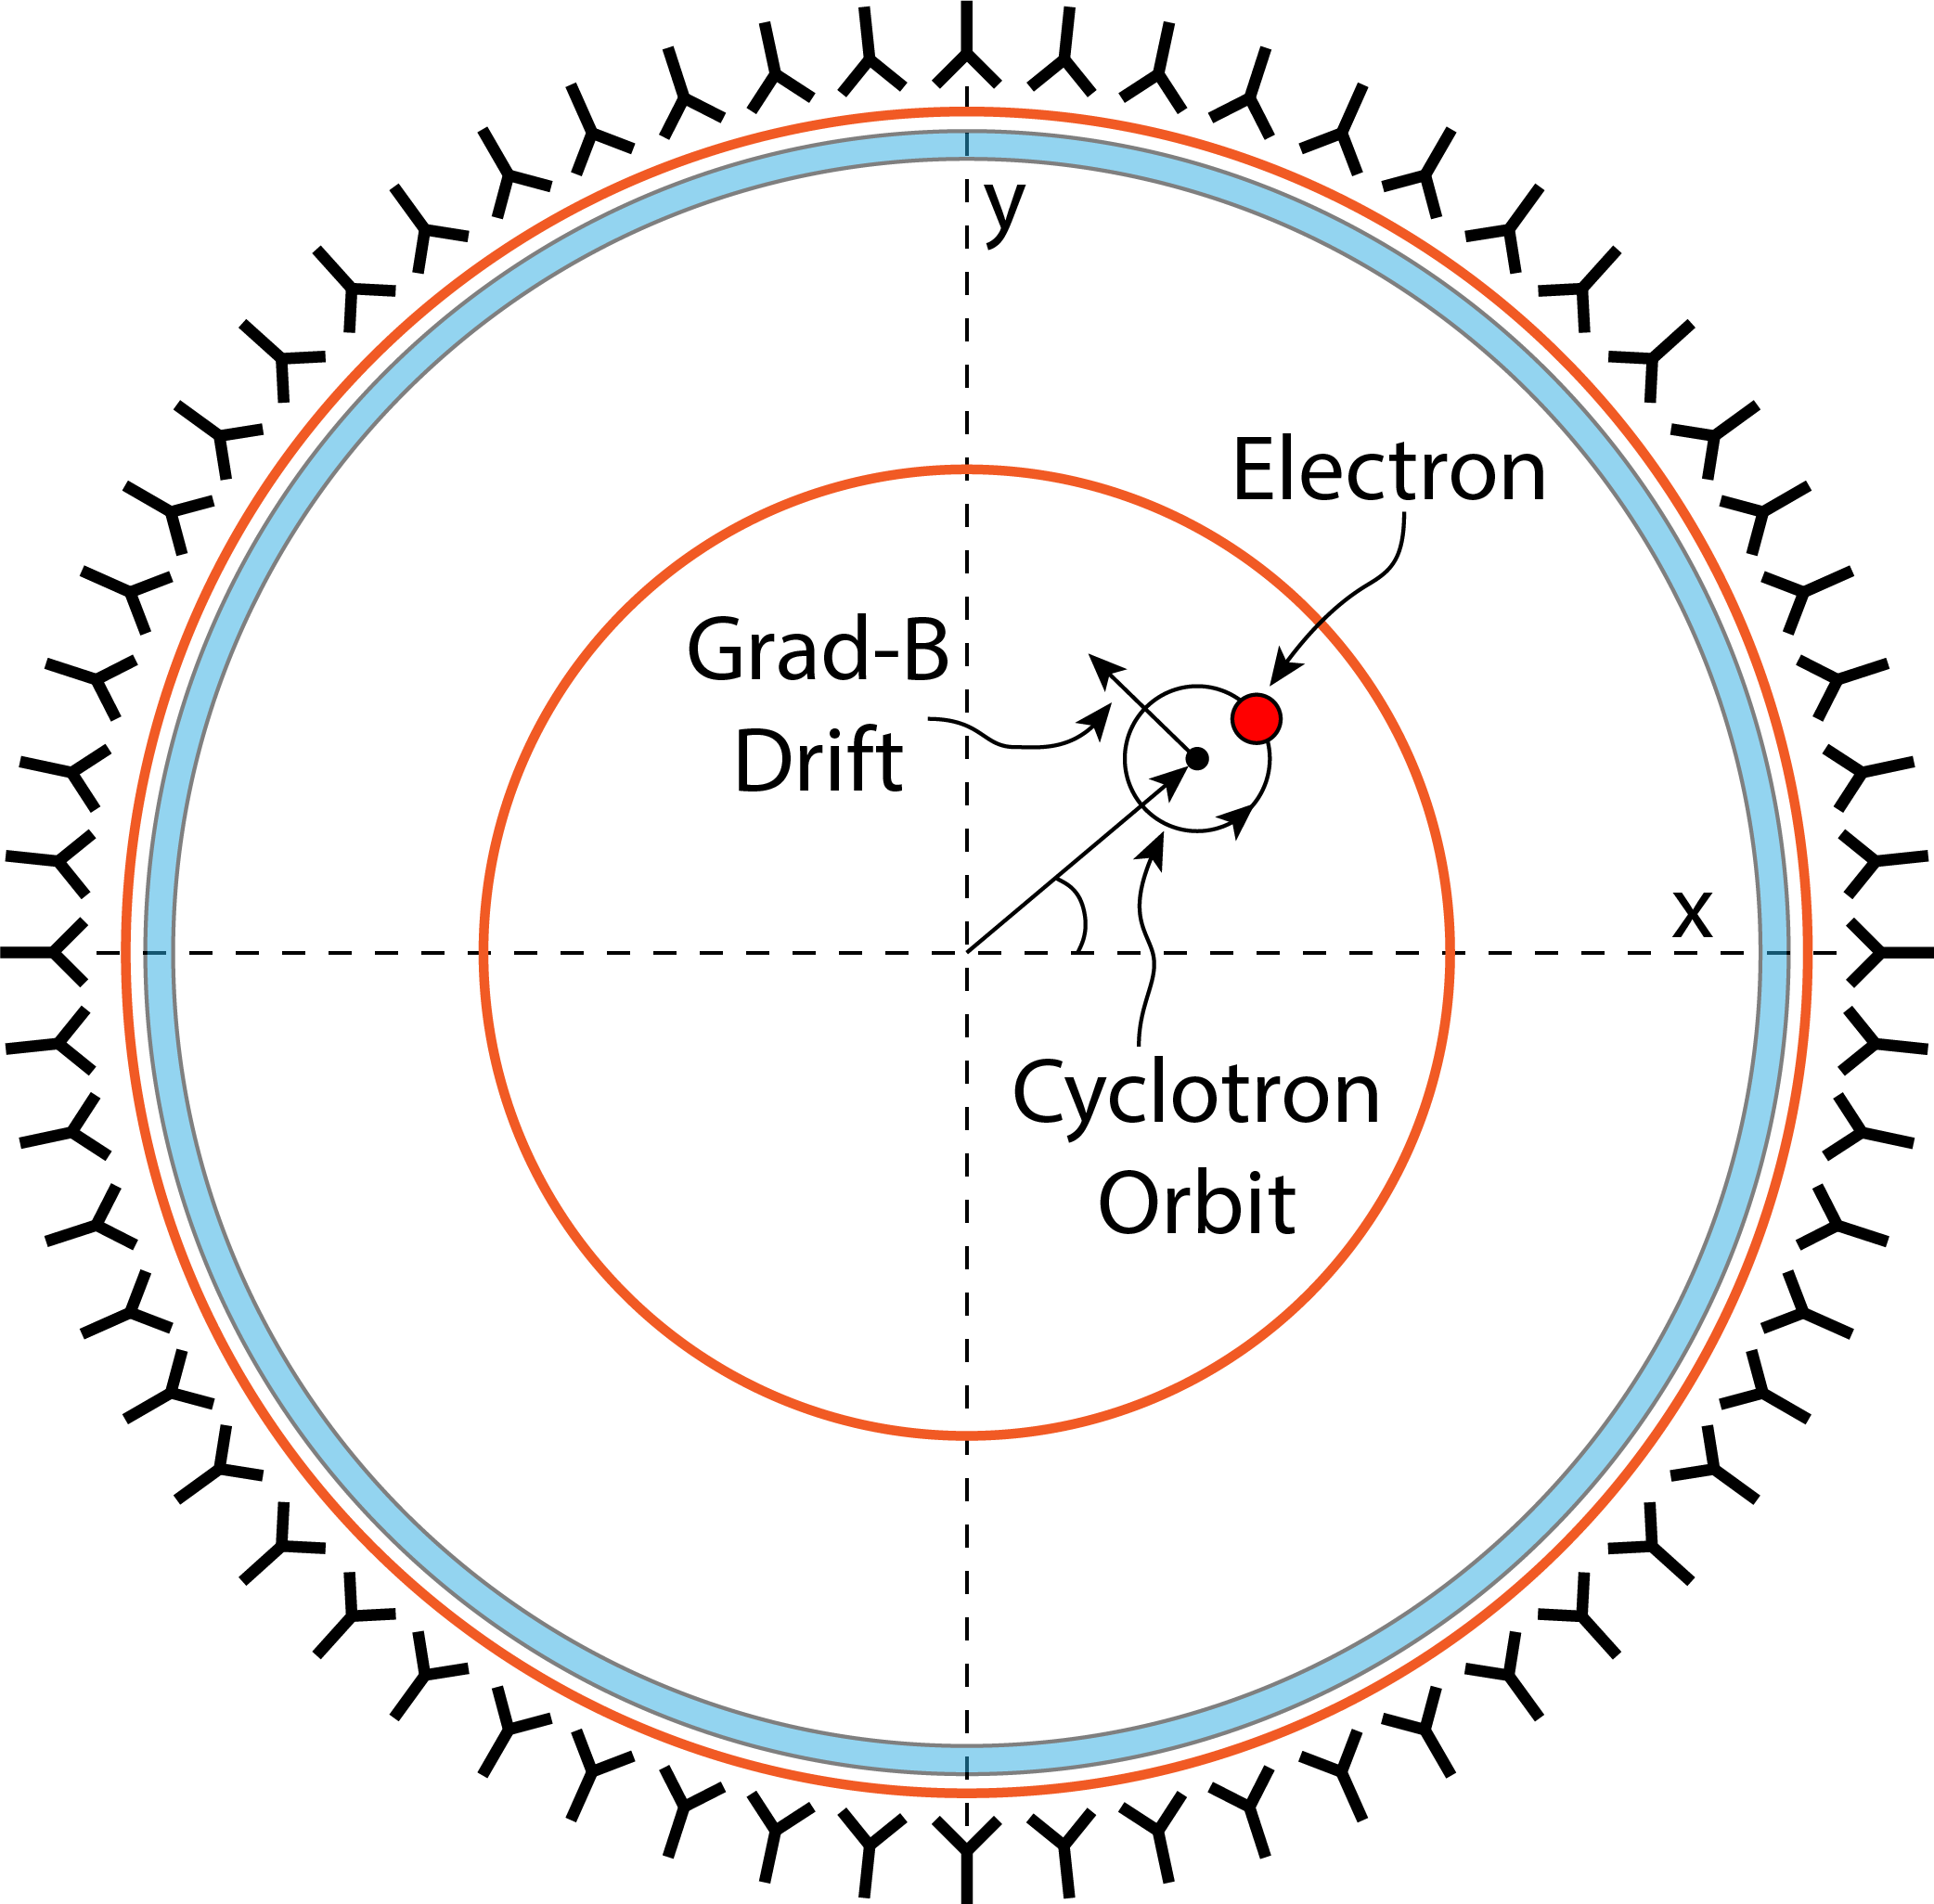
\includegraphics[width=0.9\textwidth]{figs/Chapter-4/230328_deepfilter_paper_apparatus_concept_top_v2.png}
        \caption{Top-down view.}
        \label{fig:apparatus_concept_top}
    \end{subfigure}
    \begin{subfigure}{0.48\textwidth}
        \centering
        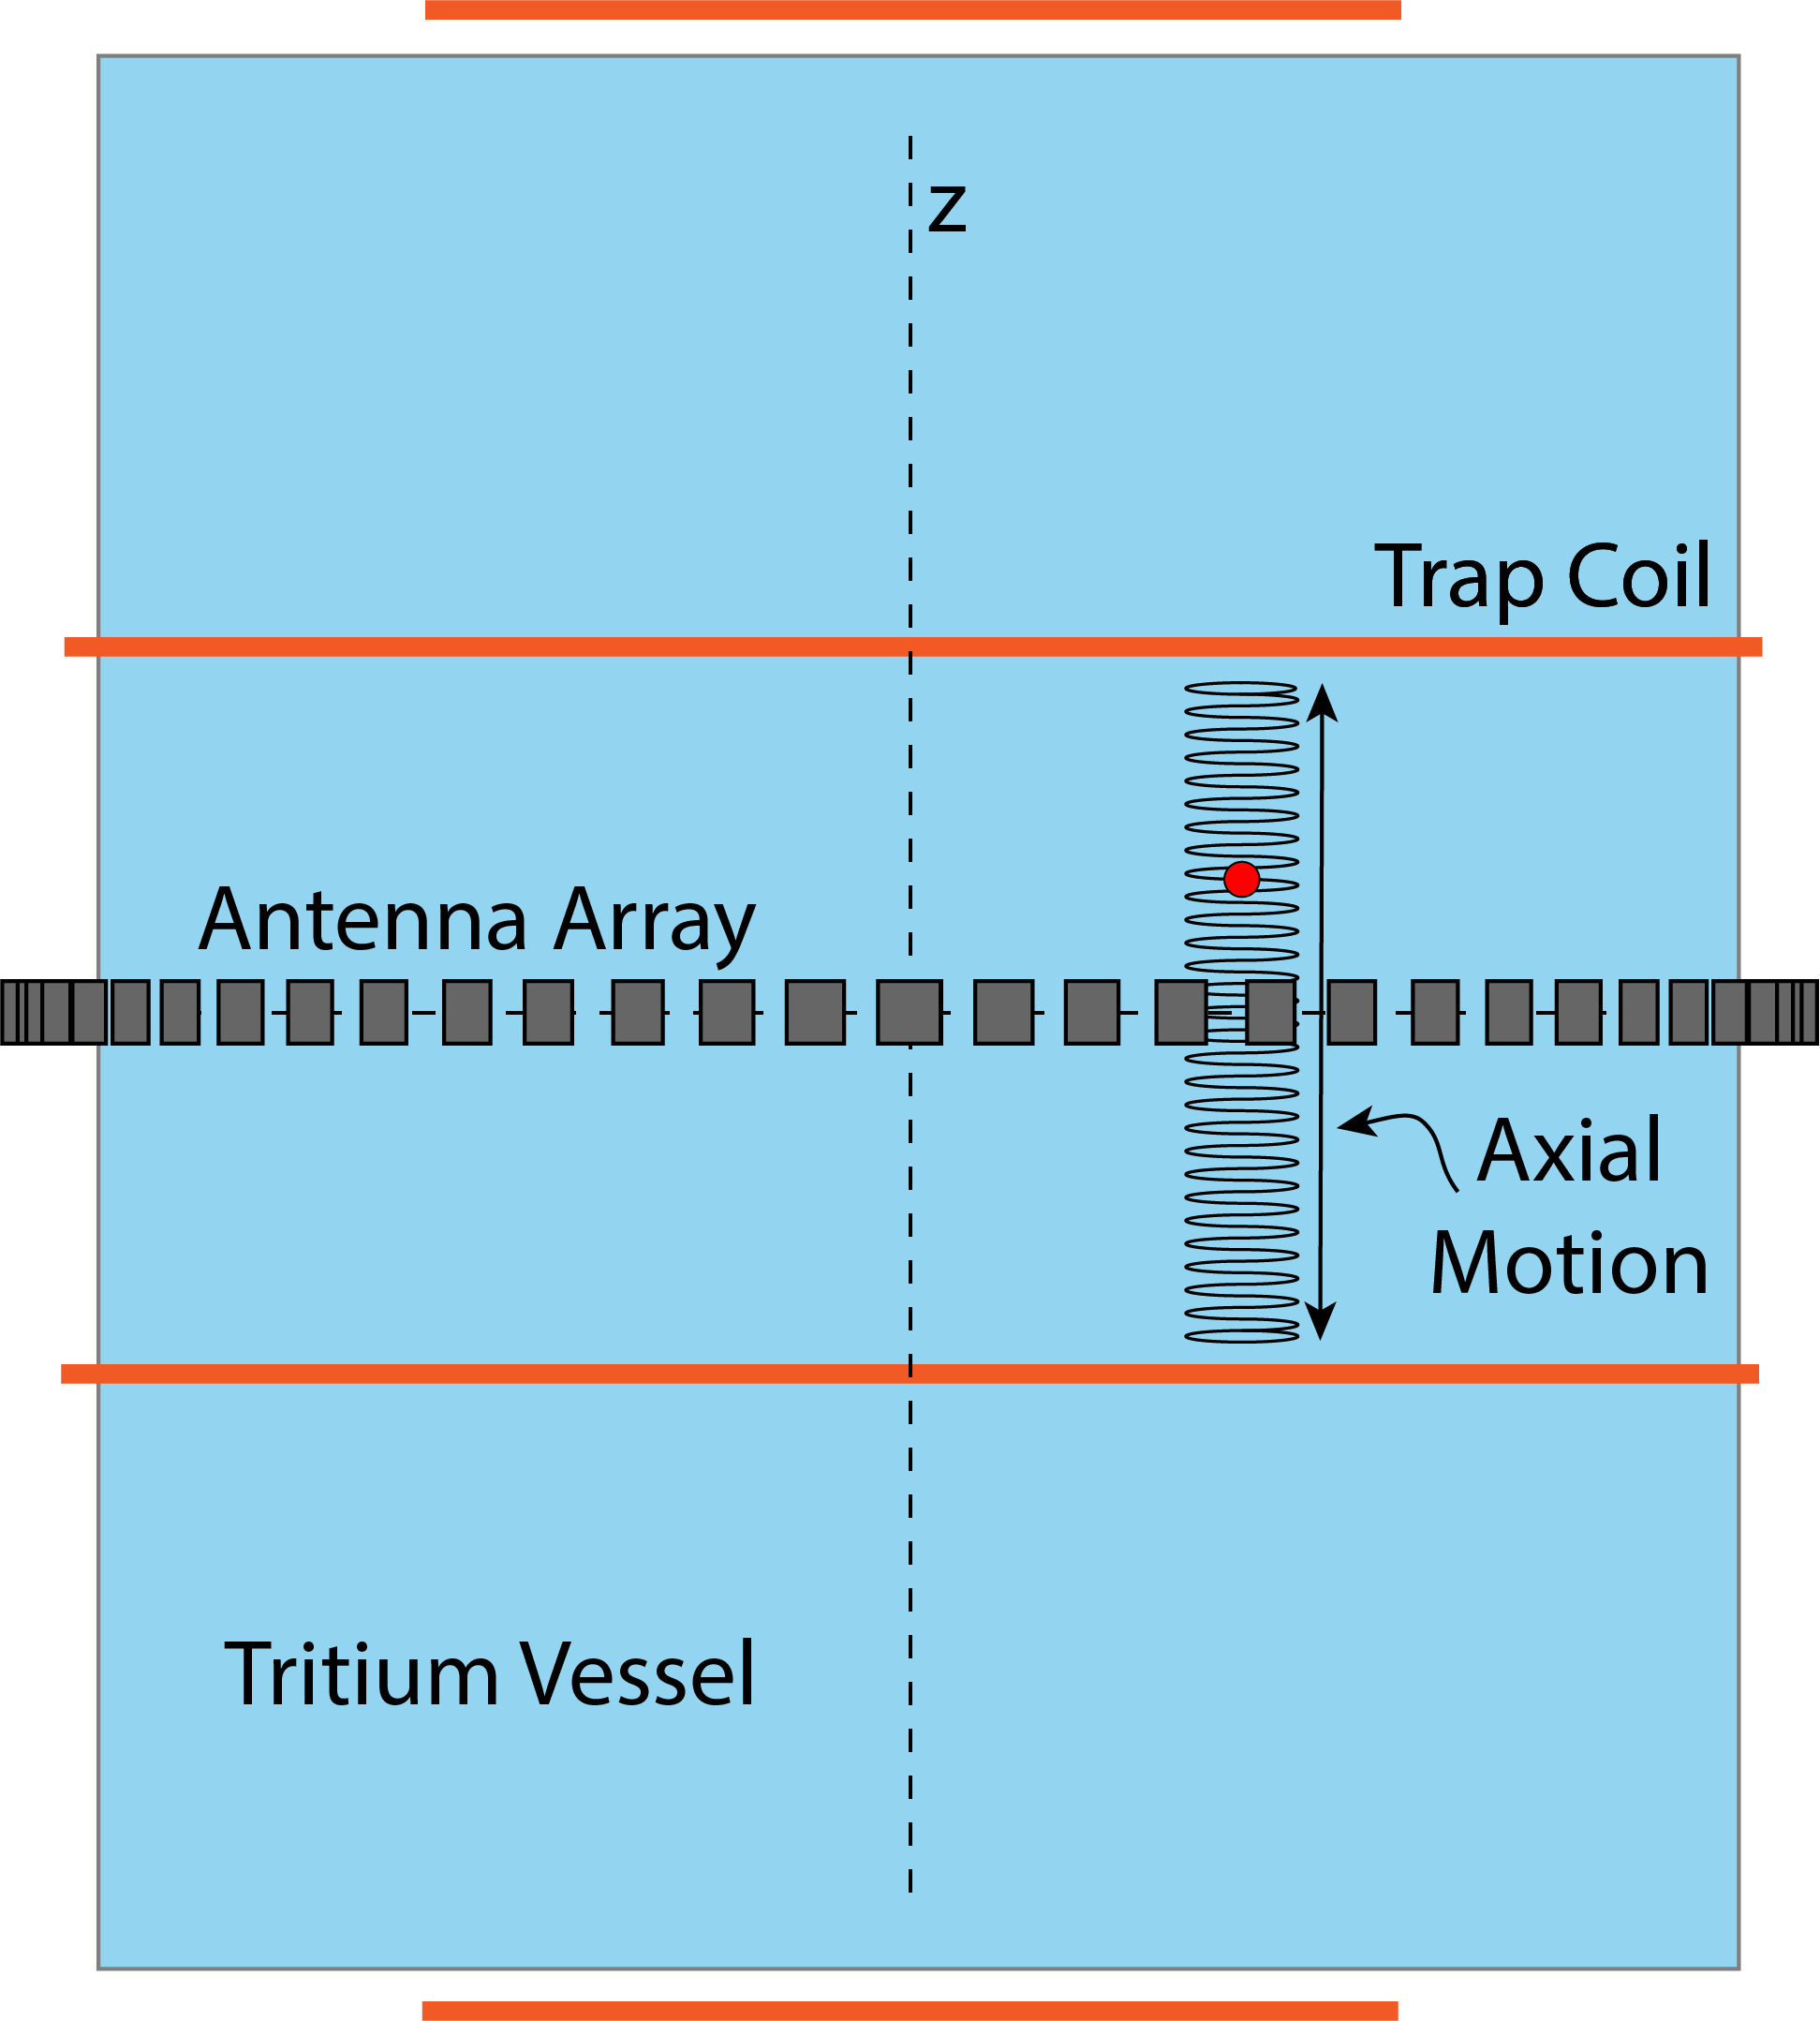
\includegraphics[width=0.9\textwidth]{figs/Chapter-4/230328_deepfilter_paper_apparatus_concept_side_v2.png}
        \caption{Side view.}
        \label{fig:apparatus_concept_side}
    \end{subfigure}
    \caption{An illustration of the conceptual design for the FSCD. The antenna array geometry consists of a 20~cm interior diameter with 60 independent antenna channels arranged evenly around the circumference. The nominal antenna design is sensitive to radiation in the frequency range of 25-26~GHz, which corresponds to the cyclotron frequency of electrons emitted near the tritium beta-spectrum endpoint in a 0.96~T magnetic field. The array is located at the center of the magnetic trap produced by a set of current-carrying coils.}
    \label{fig:apparatus_concept}
\end{figure}


% section 2
\subsection{Signal Detection with Antenna Array CRES}
\label{sec:real-time-triggering}


\subsubsection{Antenna Array and Data Rate Estimates}
\label{sec:aa-and-daq}

In order to explore the potential of antenna array CRES for neutrino mass measurement, the Project 8 Collaboration has developed a conceptual design for a prototype antenna array CRES experiment \cite{p8PanicProc,p8snowmass2022}, called the Free-space CRES Demonstrator or FSCD (see Figure \ref{fig:apparatus_concept}). The FSCD design consists of a single ring of antennas, which is the simplest form of a uniform circular array configuration, to surround a radio-frequency (RF) transparent tritium gas vessel. A stand-alone version of this antenna array has been built and tested by the Project 8 collaboration \cite{p8jugaad} to validate simulations of the array radiation pattern and beamforming algorithms \cite{balanis}. In the FSCD the antenna array is positioned at the center of the magnetic trap formed by a set of electromagnetic coils, which create a local minimum in the magnetic field with a flat central region and steep walls in the radial and axial directions. The multi-coil trap design produces a trap with a larger volume than a two-coil bathtub trap or the single-coil traps used in the Project 8 Phase II experiment \cite{p8prl2023}.

When an electron is trapped its motion consists of three primary components. The component with the highest frequency is the cyclotron orbit whose frequency is determined by the size of the background magnetic field. The FSCD design assumes a background magnetic field value of approximately 0.96~T, which results in cyclotron frequencies of approximately 26~GHz for electrons with kinetic energies near the tritium beta-spectrum endpoint. The component with the next highest frequency is the axial oscillation experienced by electrons with pitch angles\footnote{Pitch angle is defined as the angle of the particle's total momentum with respect to the local magnetic field.} of less than $90^\circ$ as they move back and forth between the trap walls \cite{p8pheno}. Typical oscillation frequencies are on the order of $\sim10$ MHz, which results in an oscillation period that is a factor of $\sim10^2$ smaller than the observation time needed for precise measurement of the cyclotron frequency. Therefore, the axial extent of the electron's motion is unknown, and the electron is treated as if it is located in the average axial position at the bottom of the magnetic trap. The component of motion with the smallest frequency is the grad-B drift caused by radial field gradients in the trap, producing an orbit of the electron around the central axis of the trap with a frequency on the order of a few kHz, dependent on the pitch angle and the radial position of the electron. 

Each component of motion influences the shape of the cyclotron radiation signals received by the antenna array, therefore, the data acquisition (DAQ) system must be properly designed in order to resolve the effects of the cyclotron, pitch angle, and grad-B motions on the signal shape. Frequency down-conversion allows for sampling of the CRES signals with a bandwidth of 200~MHz, which must be large enough to contain all sidebands produced by pitch angle modulation. The noise temperature for the FSCD can be estimated using RF link-budget analysis, which depends upon the physical temperature of the experiment as well as the noise temperature of the cyrogenic amplifiers. The analysis presented in this paper assumes an effective system noise temperature of $\approx 10$~K, which is achievable with cyrogenic temperatures and low-noise commercially-available HEMT amplifiers.


\begin{figure}[htbp]
    \centering
    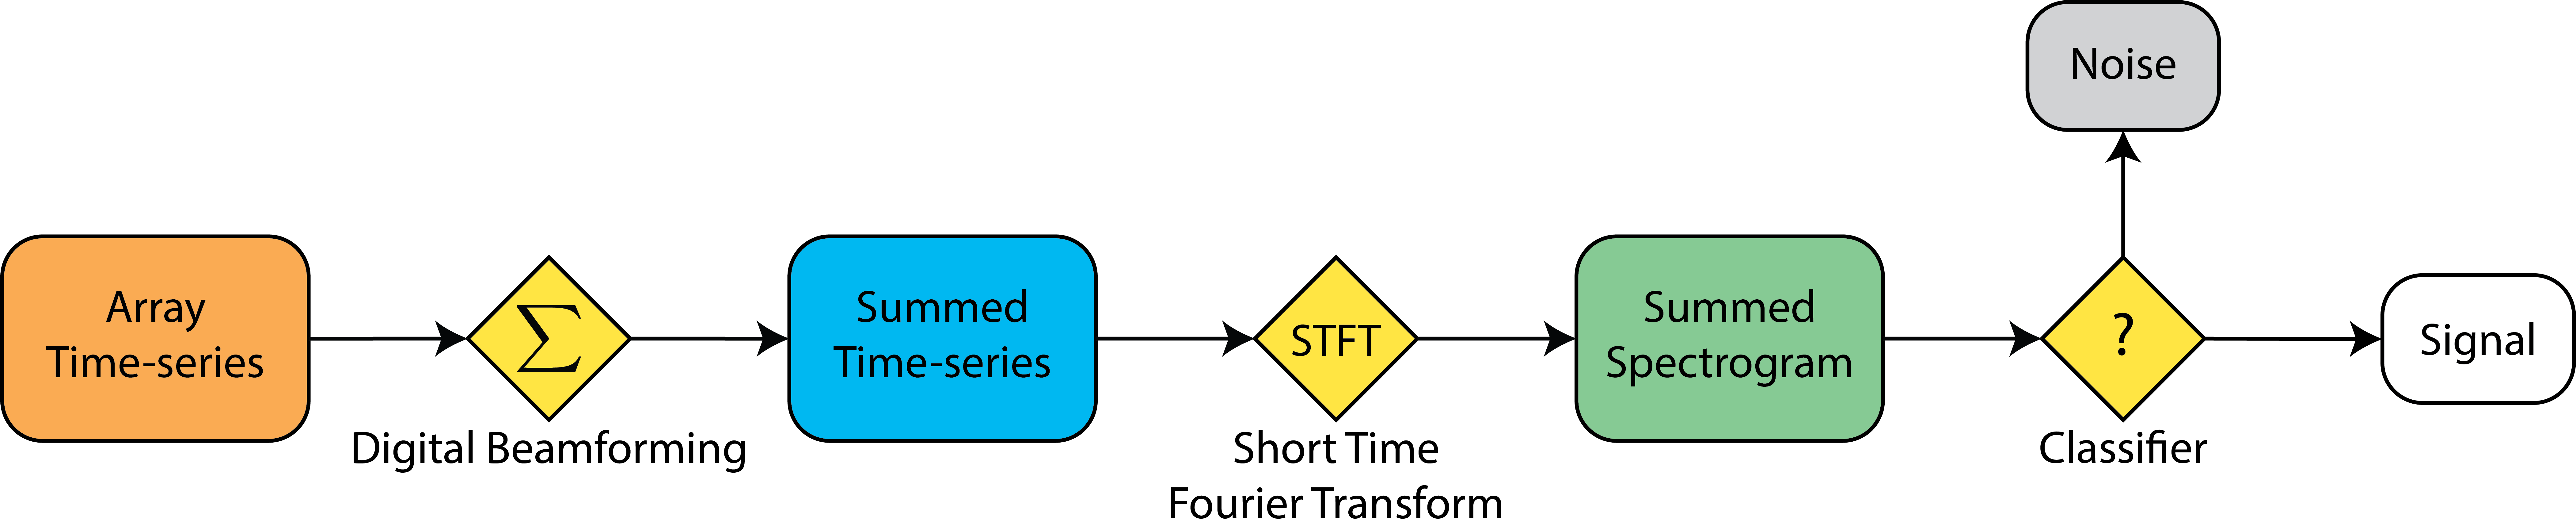
\includegraphics[width=0.9\textwidth]{figs/Chapter-4/230807_trigger_flow.png}
    \caption{A block diagram illustration of the real-time signal detection algorithm proposed for antenna array CRES reconstruction.}
    \label{fig:signal_detection_routine}
\end{figure}

A design goal for the FSCD DAQ system is to enable a significant portion of the CRES event reconstruction to occur in real-time. The estimated data volume generated by the FSCD is 1~exabyte of raw data per year of operation, with the nominal array size of 60 antennas sampled at 200~MHz, which would be prohibitive to store for offline processing. Therefore, it is ideal to perform some CRES event reconstruction in real-time so that it is possible to save a reduced form of the data for offline analysis.

The first step of the real-time reconstruction would be a real-time signal detection algorithm, which is the focus of this paper. The basic approach consists of three operations performed on the time-series data blocks including digital beamforming, a short-time Fourier transform (STFT), and a binary classification algorithm to distinguish between data that consists of signal plus noise (Signal) and data that is purely noise (see Figure \ref{fig:signal_detection_routine}).

\subsubsection{Real-time Signal Detection}
\label{sec:bf-and-stft}

\begin{figure}[htbp]
    \centering
    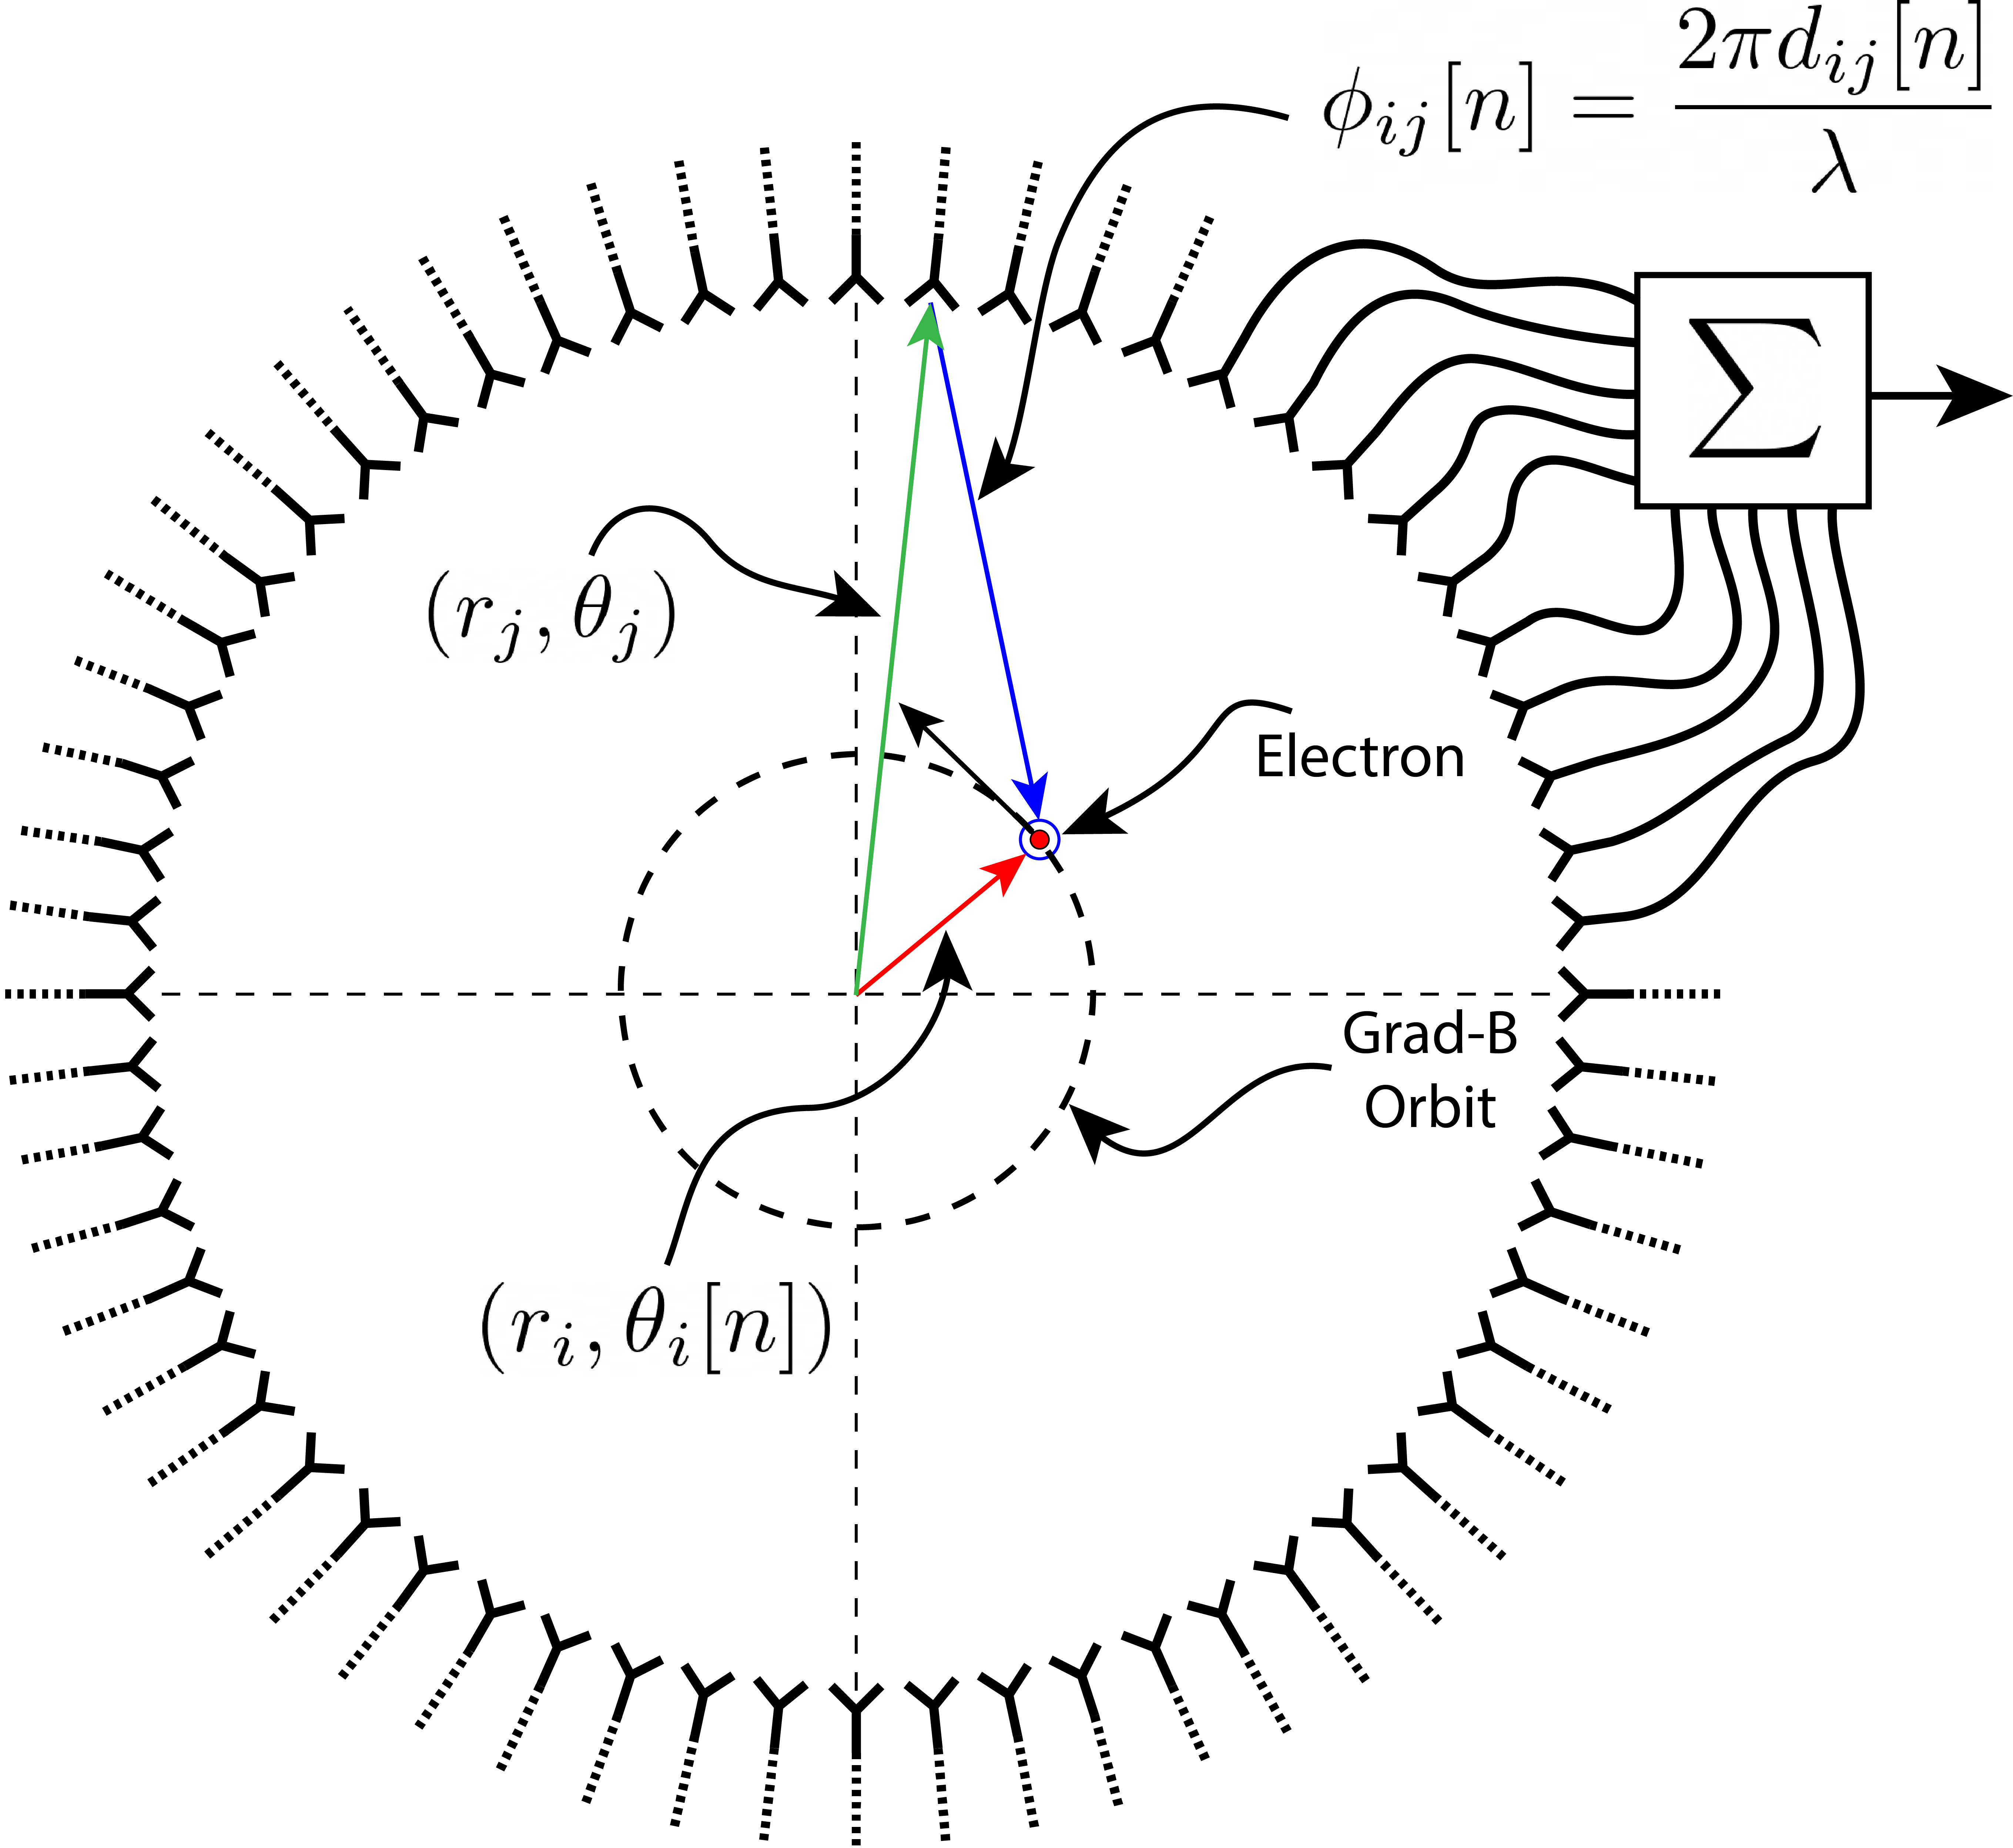
\includegraphics[width=0.65\textwidth]{figs/Chapter-4/230803_beamforming_diagram.png}
    \caption{An illustration of the digital beamforming procedure. The blue arrow indicates the distance from the beamforming position to the antenna. In the configuration depicted the actual position of the electron matches the beamforming position, therefore, one expects constructive interference when the phase shifted signals are summed. To prevent the electron's grad-B motion from moving the electron off of the beamforming position, the beamforming phases include time-dependence to follow the trajectory of the electron in the magnetic trap.}
    \label{fig:chap4-beamforming}
\end{figure}

The first step in the real-time detection algorithm is digital beamforming, which is a phased summation of the signals received by the array (see Figure \ref{fig:chap4-beamforming}). The phase shifts correspond to the path length differences between a spatial beamforming position and each antenna such that, when there is an electron located at the beamforming position, all the signals received by the array constructively interfere. Since one does not know a priori where an electron will be produced in the detector, a grid of beamforming positions is designed to cover the entire azimuthal plane where electrons can be trapped. The phased summation is performed for all points in the grid at each time step. As discussed in Section \ref{sec:aa-and-daq}, the axial oscillation of the electrons prevents one from resolving its position along the z-axis, therefore, the beamforming grid need only cover the possible positions of the electron in the two-dimensional plane defined by the antenna array. 

Mathematically, digital beamforming can be expressed as
\begin{equation}
    y_i[n] = \sum_{j=1}^{N_\mathrm{ant}}\Phi_{ij}[n]x_j[n],
    \label{eq:beamforming}
\end{equation}
where $x_j[n]$ is the voltage sampled at antenna $j$ at time $n$, $\Phi_{ij}[n]$ is a matrix element from the time-dependent beamforming phase shift matrix, and $y_i[n]$ is the summed time-series for beamforming position $i$. The elements of the beamforming phase shift matrix can be expressed as a weighted complex exponential
\begin{equation}
    \Phi_{ij}[n]=A_{ij}[n]\exp{\left(i\phi_{ij}[n]\right)},
\end{equation}
where the weight $A_{ij}$ accounts for the relative power increase for antennas that are closer to the position of the electron, and $\phi_{ij}$ is the total beamforming phase shift for the $j$-th antenna and the $i$-th beamforming position. 

The beamforming phase shift is a sum of two terms
\begin{equation}
    \phi_{ij}[n]=\frac{2\pi d_{ij}[n]}{\lambda}+\theta_{ij}[n],
\end{equation}
where the first term is the phase shift originating from the path length difference ($d_{ij}[n]$) between the beamforming and antenna positions, which are represented by the vectors $(r_j,\theta_j)$ and $(r_i,\theta_i[n])$ (see Figure \ref{fig:chap4-beamforming}), and the second term is the angular separation ($\theta_{ij}[n]$) of the two positions. The angular separation enters into the beamforming phase due to an effect caused by the circular cyclotron orbit of the electron that produces radiation whose phase is linearly dependent on the relative azimuthal position of the antenna \cite{nb_thesis, p8synca}. The time-dependence of the beamforming phases corrects for the effects of the grad-B drift, which cause the guiding centers of electrons to orbit the center of the magnetic trap. The correction adds a linear time-dependence to the azimuthal beamforming position,
\begin{equation}
    \theta_{ij}[n]=\theta_j-\theta_i[n] = \theta_j - \omega_{\nabla B}t[n]+\theta_{i}[0],
\end{equation}
where $\theta_j$ is the fixed azimuthal position of antenna $j$, $\theta_{i}[0]$ is the starting azimuthal coordinate of the beamforming position, $t[n]$ is the time vector, and $\omega_{\nabla B}$ is the grad-B drift frequency, which allows the beamforming phases to track the XY-position of the guiding center. Predicting accurate values of $\omega_{\nabla B}$ for a specific trap and set of kinematic parameters can be done with simulations, which are performed using the Locust software package \cite{p8locustpaper} developed by Project 8.

\begin{figure}[ht]
    \centering
    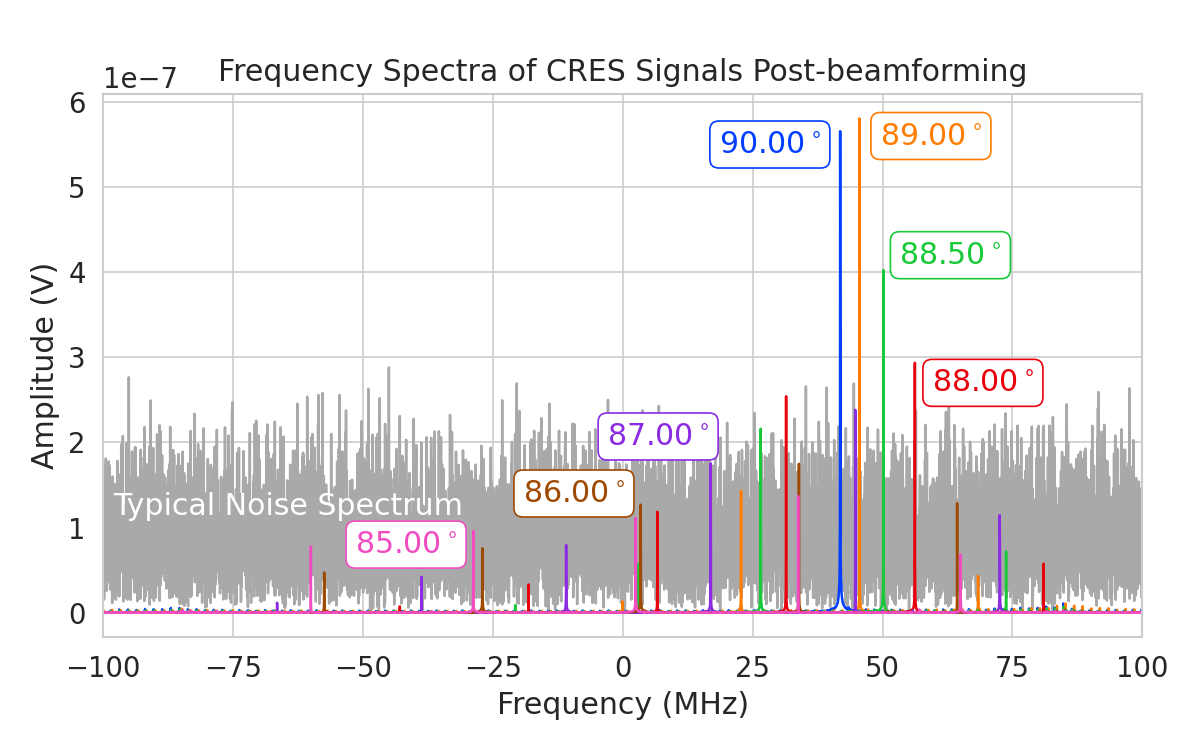
\includegraphics[width=.7\textwidth]{figs/Chapter-4/230927_cres_signal_post_bf_examples.png}
    \caption{Frequency spectra of simulated CRES events in the FSCD magnetic trap after beamforming. The depicted frequency range has been down-converted using a local oscillator frequency of 25.86~GHz. The signal of a $90^\circ$ electron consists of a single frequency component that is clearly detectable using a power threshold on the frequency spectrum. This power threshold remains effective for signals with relatively large pitch angles such as $89.0^\circ$, which are composed of a main carrier and a few small sidebands. Signals with smaller pitch angles, below about $88.5^\circ$, are dominated by sidebands such that no single frequency component can be distinguished from the noise with sufficient statistical confidence using a power threshold.
    }
    \label{fig:signal_post_bf_example}
\end{figure}

After digital beamforming, a STFT is applied to the summed time-series to obtain the signal frequency spectrum (see Figure \ref{fig:signal_post_bf_example}). The sparseness of CRES signals in the frequency domain makes this representation better than the time domain for the purposes of signal detection. The frequency spectra of CRES signals are well-approximated by a frequency and amplitude modulated sinusoidal whose carrier frequency increases as a linear chirp \cite{p8pheno}. The modulation is caused by the axial oscillation of the electron in the magnetic trap, and the linear chirp is caused by the energy loss due to cyclotron radiation, which results in a relatively slow increase in the frequency components of the CRES signal over time. A typical CRES signal increases in frequency by approximately 15~kHz during the standard Fourier analysis window of 40.96~$\mu$sec, which is smaller than the frequency bin width for a 200~MHz sample rate. Therefore, when considering a single frequency spectrum it is justifiable to neglect the effects of the linear frequency chirp. 

The majority of the CRES signal power for electrons in the FSCD trap is contained in a single frequency component when the electron has a pitch angle $\gtrsim 88.5^\circ$. The remaining signal power is distributed between a small number of sidebands with amplitudes proportional to the electron's axial modulation (see Figure \ref{fig:signal_post_bf_example}). Signal detection for these pitch angles is straightforward using a simple power threshold on the STFT, since the amplitude of the main signal peak is well above the thermal noise spectrum. However, as the pitch angle of the electron is decreased below $88.5^\circ$, the maximum amplitude of the frequency spectrum becomes comparable to typical noise fluctuations. At this point, the power threshold trigger is no longer able to distinguish between signal and noise leading to a reduction in detection efficiency, which is directly linked to the neutrino mass sensitivity of the FSCD. Because the distribution of electron pitch angles is effectively uniform, utilizing a signal detection algorithm that can improve efficiency for pitch angles less than $88.5^\circ$ can lead to improvements in the neutrino mass sensitivity of the FSCD. 


\subsection{Signal Detection Algorithms}
\label{sec:classifiers}

Modeling detection performance requires one to pose the signal detection problem in a consistent manner. The approach taken here uses the frequency spectra obtained from a STFT applied to beamformed time-series from the FSCD to perform a binary hypothesis test. Mathematically, this is expressed as,
\begin{align}
    \mathcal{H}_0 & : y[n]=\nu[n]\\
    \mathcal{H}_1 & : y[n]=x[n]+\nu[n].
\end{align}
Under hypothesis $\mathcal{H}_0$ the vector representing the frequency spectrum ($y[n]$) is composed only of complex white Gaussian noise (cWGN, $\nu[n]$) with total variance $\tau$, and under hypothesis $\mathcal{H}_1$ the frequency spectrum is composed of a CRES signal ($x[n]$) with added cWGN. The dominant noise source for the FSCD is expected to be thermal Nyquist-Johnson noise, which is well approximated by a cWGN distribution. The hypothesis test is performed by calculating the ratio between the log-likelihood probability distributions for the classifier under $\mathcal{H}_1$ and $\mathcal{H}_0$, which is the standard Neyman-Pearson approach to hypothesis testing \cite{detection_theory}. The output of the log-likelihood ratio test is called the test statistic, which is used to assign the data as belonging to the noise or signal classes using a decision threshold on the test statistic value. 

In practice, the decision threshold is selected by finding the value of the test statistic that guarantees a tolerable rate of false positives. Given this false positive rate (FPR), one attempts to find a classifier that maximizes the true positive rate (TPR), which is the probability of correctly identifying if a piece of data contains a signal. Because FSCD signal classifiers will be used to evaluate the spectra of $O(10^2)$ beamforming positions every 40.96~$\mu$sec, there is a requirement that the signal classifiers with FPR significantly smaller than 1\% to minimize the number of false positives that must be filtered out in later stages of the CRES signal reconstruction chain.

\subsubsection{Power Threshold}

The power threshold detection algorithm uses the maximum amplitude of the frequency spectrum as the detection test statistic. Consider the $\mathcal{H}_0$ hypothesis where the signal is pure cWGN. The performance of the power threshold can be modeled by first analyzing a single bin in the frequency spectrum. The probability that the amplitude of a frequency bin falls below the decision threshold is given by the Rayleigh cumulative distribution function (CDF),
\begin{equation}
    \mathrm{Ray}(|z|;\tau)=1-\exp{\left(-|z|^2/\tau\right)},
\end{equation}
where $|z|$ represents the value of the decision threshold on the spectrum amplitude, and $\tau$ is the cWGN variance (defined below, Equation \ref{eq:cwgn_var}). Because the noise samples are independent and identically distributed (IID), the probability that all bins in the frequency spectrum fall below the threshold is the joint CDF formed by the product of each individual frequency bin CDF,
\begin{equation}
    F_0(|z|;\tau, N_\mathrm{bin})=\mathrm{Ray}(|z|;\tau)^{N_\textrm{bin}}.
    \label{eq:fft_spectrum_cdf0}
\end{equation}
Finally, the PDF for the power threshold classifier can be obtained by differentiating Equation \ref{eq:fft_spectrum_cdf0}.

The noise of a beamformed frequency spectrum is a summation of all the noise samples from the array channels. The received Nyquist-Johnson noise power for a single antenna is given by $k_BT\Delta f$, where $k_B$ is Boltzmann's constant, $T$ is the system noise temperature, and $\Delta f$ is the sample rate. The beamformed noise variance is increased by a factor of $N_\textrm{ch}$, where $N_\textrm{ch}$ is the number of antennas, caused by the summation of incoherent noise samples, however, the noise variance per frequency bin is decreased by a factor equal to the number of samples in the STFT ($N_\textrm{FFT}$). The amplitude weights applied during beamforming also affect the noise variance in a position dependent way, since the analysis presented in this work focuses on only a single spatial position (see Section \ref{sec:method}), it was decided to weigh the signal in each channel equally, which results in the same noise variance for all beamforming positions. The final expression for the noise variance that describes a beamformed frequency spectrum is given by 
\begin{equation}
    \tau = k_BT\Delta fN_\textrm{ch}R/N_\textrm{FFT},
    \label{eq:cwgn_var}
\end{equation}
where the system impedance ($R$) has been used to convert from power to voltage-squared. 


\begin{figure}[htbp]
    \centering
    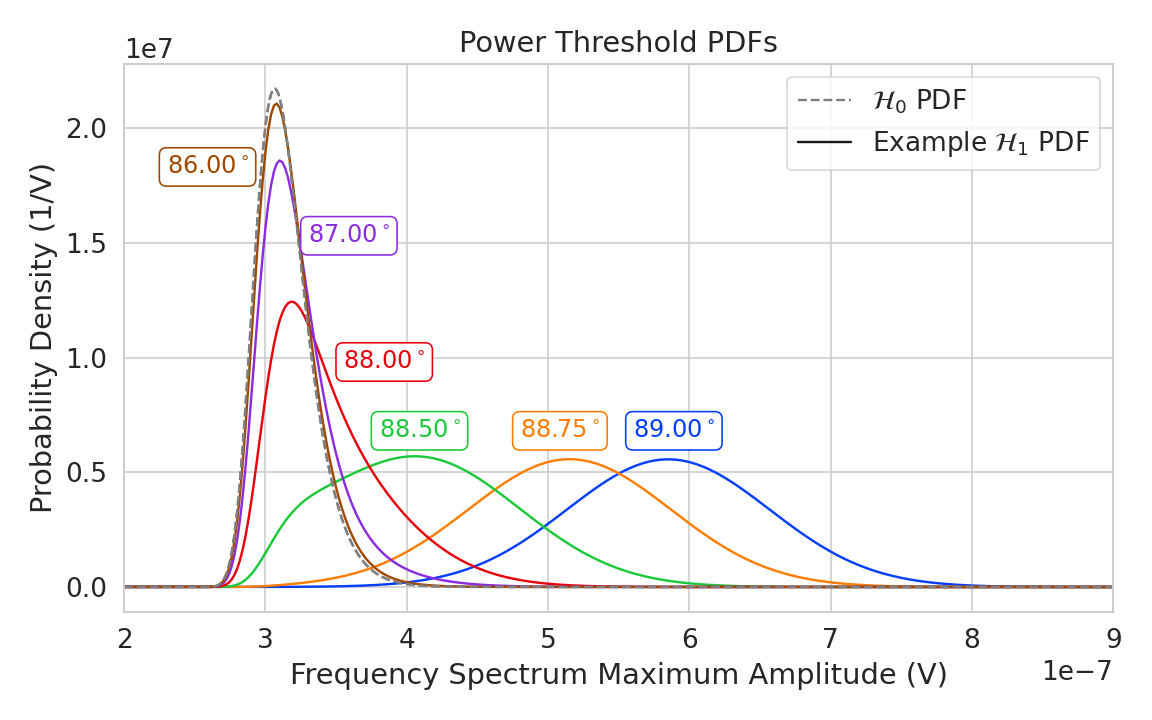
\includegraphics[width=0.7\textwidth]{figs/Chapter-4/230915_fft_power_threshold_pdf_by_pitch.png}
    \caption{PDFs of the power threshold test statistic for CRES signals with various pitch angles as well as the PDF for the noise-only ($\mathcal{H}_0$) case. As the pitch angle is decreased the $\mathcal{H}_1$ PDFs converge towards the noise PDF, which indicates that the power threshold is unable to distinguish between signal and noise. }
    \label{fig:fft_pdf}
\end{figure}

Similar to $\mathcal{H}_0$, the power threshold classifier distribution under $\mathcal{H}_1$ is calculated by combining the distributions of individual frequency bins; however, the frequency bins that contain signal must be treated separately. The probability that the amplitude of a frequency bin which contains both signal and noise is below the decision threshold is described by a Rician CDF \cite{detection_theory}
\begin{equation}
    \mathrm{Rice}(|z|;\tau, |x_k|)=1-\int_{|z|}^{\infty}{d|\Tilde{z}|\frac{2|\Tilde{z}|}{\tau}\exp{\left(-\frac{|\Tilde{z}|^2+|x_k|^2}{\tau}\right)}\mathcal{I}_0\left(\frac{2|\Tilde{z}||x_k|}{\tau}\right)},
\end{equation}
where $|x_k|$ defines the amplitude of the $k$-th component of the signal frequency spectrum. The CDF that describes the probability that the entire spectrum falls below the decision threshold is the product of both signal and noise CDFs,
\begin{equation}
    F_1(|z|;\tau, \mathbf{x}_s, N_\mathrm{bin}, N_s)=\mathrm{Ray}(|z|;\tau)^{N_\mathrm{bin}-N_s}\prod_{k=1}^{N_s}{\mathrm{Rice}(|z|;\tau, \left|\mathbf{x}_s[k]\right|)}.
    \label{eq:fft_spectrum_cdf1}
\end{equation}
The first half of Equation \ref{eq:fft_spectrum_cdf1} is the contribution from the bins in the frequency spectrum that contain only noise, and the second half is the product of the Rician CDFs for the frequency bins that contain signal peaks with noise-free amplitudes of $\mathbf{x}_s=\left[x_1,\ldots, x_{N_s}\right]$, where $N_s$ is the number of non-zero frequency peaks in the CRES signal spectrum. Figure \ref{fig:fft_pdf} shows plots of example PDFs under $\mathcal{H}_1$ and $\mathcal{H}_0$.

\subsubsection{Matched Filtering}

\label{sec:classifiers-mf}

The shape of a CRES signal between random scattering events with the background gas is completely determined by the initial conditions of the electron, which implies that it is possible to apply matched filtering as a signal detection algorithm. A matched filter uses the shape of the known signal, which is called a template, to filter the incoming data by computing the convolution between the signal and the data \cite{detection_theory}. The matched filter is the optimal detector, which means it achieves the maximum TPR for a particular FPR, under the assumption that the signal is perfectly known and the noise is Gaussian distributed. Since CRES signals have an unknown shape but are deterministic, the matched filter can be applied by using simulations to generate a large number of signal templates, called a "template bank", which spans the parameter space of possible signals. Then at detection time, the template bank is used to identify signals by performing the matched filter convolution for each template in an exhaustive search.

CRES signals are highly periodic in nature. In such cases, it is advantageous to utilize the convolution theorem to replace the matched filter convolution with an inner product in the frequency-domain. Using the convolution theorem, the matched filter test statistic is given by
\begin{equation}
    \mathcal{T}=\max_{m}\left|\sum_{n=0}^{N_\mathrm{bin}}h_m^\dagger[n]y[n]\right|,
    \label{eq:mf_test_stat}
\end{equation}
where $h_m^\dagger[n]$ is the complex conjugate of the $m$-th signal template and $y[n]$ is the frequency spectrum of the beamformed time-series. 

\subsubsection*{Single Template}

The approach to deriving PDFs that describe the matched filter template bank will be to first derive PDFs for $\mathcal{H}_0$ and $\mathcal{H}_1$ in the case of a single template and use these solutions to create PDFs that describe the multi-template case. In the case when the template bank consists of only a single template it is possible to derive an exact analytical form for the PDF. Consider the $\mathcal{H}_1$ case, where the equation describing the matched filter test statistic, also known as the matched filter score, becomes
\begin{equation}
    \mathcal{T}=\left|\sum_{n=0}^{N_\mathrm{bin}}h^\dagger[n]y[n]\right|.
    \label{eq:mf_inner_prod_1}
\end{equation}
Each noisy frequency bin is a sum of signal and cWGN, which means $y[n]$ is also a Gaussian distributed variable. Therefore, the value of the inner product between the template and the data is also a complex Gaussian variable; and, since the matched filter score is the magnitude of this inner product, it must follow a Rician distribution. 

The matched filter template $\mathbf{h}$ is a simulated signal ($\mathbf{x}_h$) with a normalization factor
\begin{equation}
    \mathbf{h}=\frac{\mathbf{x}_h}{\sqrt{\tau|\mathbf{x}_h|^2}},
    \label{eq:appendix-mf-template}
\end{equation}
where $\tau$ is the noise variance. Inserting this into Equation \ref{eq:mf_test_stat} and expressing the data as a sum between a signal and a cWGN vector yields,
\begin{equation}
    \mathcal{T}=\frac{1}{\sqrt{\tau|\mathbf{x}_h|^2}}\left|\sum_{n=1}^{N_\mathrm{bin}}{x_h^\dagger[n]x[n]} + \sum_{n=1}^{N_\mathrm{bin}}{x_h^\dagger[n]\nu[n]}\right|.
    \label{eq:appendix-eqn-1}
\end{equation}

The first term is a scalar product between the signal and template vectors and the second term is a complex Gaussian distributed variable with variance one. For the purposes of identifying the statistical distribution, it is useful to rewrite the summation describing an inner product 
\begin{equation}
    \sum_{n=1}^{N_\mathrm{bin}}{x_h^\dagger[n]x[n]}=\mathbf{x}_h\cdot\mathbf{x}=|\mathbf{x}_h\cdot\mathbf{x}|e^{i\vartheta}\leq|\mathbf{x}_h||\mathbf{x}|e^{i\vartheta},
\end{equation}
the last step utilizes the Cauchy-Schwarz inequality, where equality is guaranteed when $\mathbf{x}=\mathbf{x}_h$. Instead of the inequality it is useful to define a quantity called "match" such that 
\begin{equation}
    |\mathbf{x}_h\cdot\mathbf{x}|e^{i\vartheta}=|\mathbf{x}_h||\mathbf{x}|\Gamma e^{i\vartheta},
\end{equation}
where the match factor $\Gamma\in[0,1]$. The match factor quantifies how well the template matches the signal.

The fact that the second term in Equation \ref{eq:appendix-eqn-1} is a random complex Gaussian variable with unity variance can be seen by noting that each of the noise samples are drawn from the complex Gaussian distribution, $\mathcal{N}(0,\tau)$. Therefore,
\begin{align}
    \frac{x_h^\dagger[n]}{\sqrt{\tau|\mathbf{x}_h|^2}}\nu[n]&\sim\mathcal{N}\left(0,\frac{x_h^\dagger[n]x_h[n]}{|\mathbf{x}_h|^2}\right),\\
    n=\sum_{n=1}^{N_\mathrm{bin}}{\frac{x_h[n]}{\sqrt{\tau|\mathbf{x}_h|^2}}\nu[n]}&\sim\mathcal{N}\left(0,\frac{\sum_{n=1}^{N_\mathrm{bin}}{x_h^\dagger[n]x_h[n]}}{|\mathbf{x}_h|^2}\right)=\mathcal{N}(0,1).
\end{align}

Equation \ref{eq:appendix-eqn-1} can now be simplified
\begin{equation}
    \mathcal{T}= \left||\mathbf{h}||\mathbf{x}|\Gamma e^{i\vartheta}+n\right|,
\end{equation}
where Equation \ref{eq:appendix-mf-template} has been used to redefine the inner product term. The quantity $|\mathbf{h}||\mathbf{x}|\Gamma$ is a real number, which is the matched filter score that one would expect if the data contained no noise. Since $\mathbf{h}$ and $\mathbf{x}$ can potentially be mismatched, $\Gamma$ is not necessarily equal to 1. The final simplification is to define $\mathcal{T}_\mathrm{0}=|\mathbf{h}||\mathbf{x}|\Gamma$, from which one obtains
\begin{equation}
    \mathcal{T}=|\mathcal{T}_\mathrm{0}e^{i\vartheta}+n|.
    \label{eq:appendix-simplified-mf-score}
\end{equation}

From Equation \ref{eq:appendix-simplified-mf-score} on can see that $\mathcal{T}$ is simply the magnitude of a complex number with added cWGN of variance 1, which follows the Rician distribution; therefore, the distribution that describes the matched filter score for a single template under $\mathcal{H}_1$ is
\begin{equation}
    P_1(w;\mathcal{T}_0) = 2w\exp{\left(-\left(w^2+\mathcal{T}_0^2 \right)\right)}I_0(2w\mathcal{T}_0).
    \label{eq:mf_pdf_1}
\end{equation}
where $I_0$ is the zeroth-order modified Bessel function of the first kind and $w$ is the value of the matched filter score decision threshold. 

The shape of the matched filter score distribution is controlled by the parameter $\mathcal{T}_0$, which is effectively the value of the matched filter score if the data contained no noise. Without noise, the data vector reduces to the signal, $\mathbf{x}$, in which case Equation \ref{eq:mf_inner_prod_1} becomes the magnitude of an inner product between two vectors. The magnitude of an inner product can be expressed in terms of the magnitudes of the vectors and a constant that describes the degree of orthogonality between them. Applying this to Equation \ref{eq:mf_inner_prod_1}, one obtains
\begin{equation}
    \mathcal{T}_0=\left|\mathbf{h}^\dagger\cdot\mathbf{x}\right| = \left|\mathbf{h}\right|\left|\mathbf{x}\right|\Gamma,
    \label{eq:ideal_mf_score}
\end{equation}
where $\Gamma$ is a number that ranges from 0 to 1 and describes the orthogonality between $\mathbf{h}$ and $\mathbf{x}$. $\Gamma$ effectively quantifies how well the template matches the unknown signal in the data.

The matched filter score PDF under $\mathcal{H}_0$ is readily obtained from Equation \ref{eq:mf_pdf_1} by setting the value of $\mathcal{T}_\mathrm{0}$ to zero, since the data contains no signal in the noise case. Doing this, one obtains a Rayleigh distribution,
\begin{equation}
    P_0(w) = 2w\exp{\left(-w^2\right)}.
    \label{eq:mf_pdf_0}
\end{equation}

\subsubsection*{Multi-template}

Equations \ref{eq:mf_pdf_1} and \ref{eq:mf_pdf_0} describe the behavior of the matched filter test statistic under $\mathcal{H}_0$ and $\mathcal{H}_1$ for a single template. However, defining a PDF that describes the matched filter test statistic in the case of multiple templates is in general a mathematically intractable problem, since there is no guarantee of orthogonality between matched filter templates. This leads to correlations between the matched filter scores of different templates, because only one sample of noise is used to compute the matched filter scores of the template bank. 

In order to proceed, it is assumed that the matched filter scores for all templates are IID variables, which allows one to ignore correlations between templates. The overall effect of this will be an underestimate of the performance of the matched filter by over-estimating the required number of templates and the magnitude of the statistical trials penalty. The magnitude of this underestimation, while it cannot be predicted in advance, can be quantified using Monte-Carlo tests of the matched filter templates and randomly generated test signals.

\begin{figure}[htbp]
    \centering
    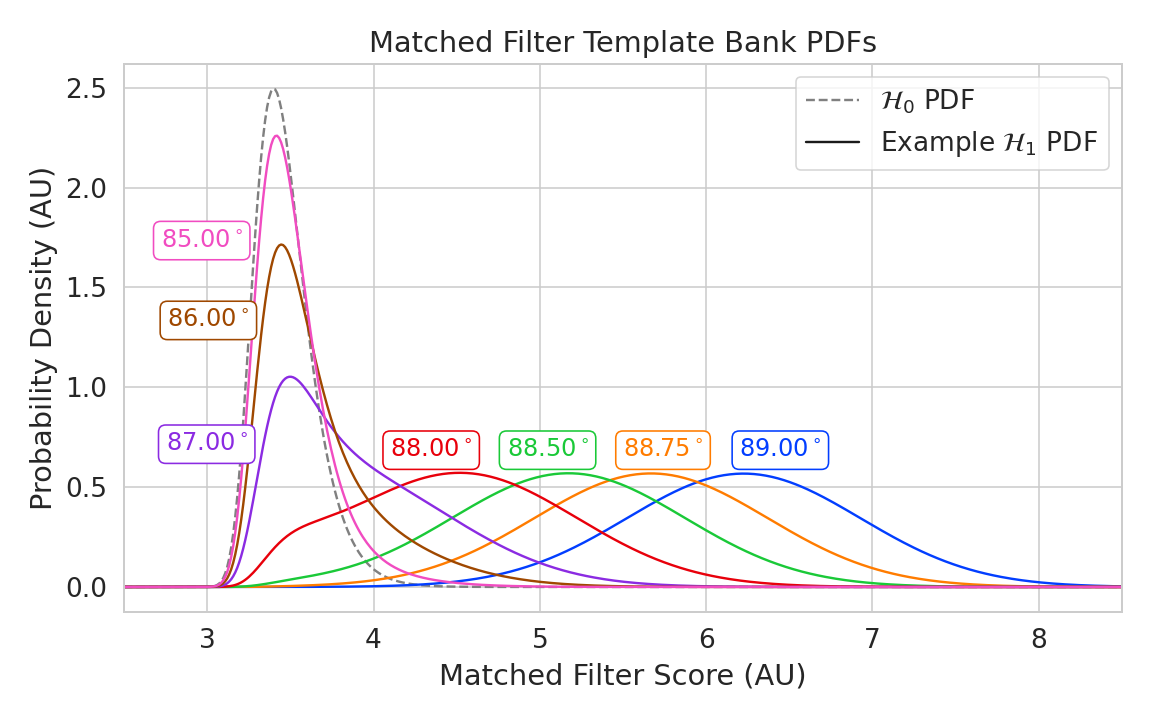
\includegraphics[width=0.7\textwidth]{figs/Chapter-4/230915_mf_pdf_by_pitch.png}
    \caption{Example PDFs that describe the matched filter template bank test statistic for CRES signals with various pitch angles, as well as the estimated PDF for the noise-only case. $10^5$ matched filter templates and perfect match between signal and template, i.e. $\Gamma=1$, is assumed. One can observe that there is greater separation between the signal PDFs and the noise PDF for the matched filter template bank compared to the power threshold. Therefore, one expects that the matched filter will have generally better detection efficiency than the power threshold.}
    \label{fig:mf_pdf}
\end{figure}

The probability that the matched filter score falls below the decision threshold under $\mathcal{H}_0$ is again given by the CDF. Because of the assumption that matched filter scores from different templates are independent, the probability that the matched filter score for all templates falls below the threshold value is simply the joint CDF, which is
\begin{equation}
    F_{0}(w) = \left(1-e^{-w^2}\right)^{N_t},
    \label{eq:mf_joint_cdf_0}
\end{equation}
where $w$ is the matched filter score threshold and $N_t$ is the number of templates. One should expect that the distribution describing the maximum score of the matched filter template bank depends on $N_t$, because with more templates there is a greater chance of a random match between the template and noise data.

The CDF that describes $\mathcal{H}_1$ is derived by starting with the CDF of the best matching template. The best matching template is simply the template that yields the largest matched filter score. The score of the best template is defined by
\begin{equation}
    \mathcal{T}_\mathrm{best}=\max_{m}\left(|\mathbf{h}_m||\mathbf{x}|\Gamma_{m}\right) = |\mathbf{h}_\mathrm{best}||\mathbf{x}|\Gamma_{\mathrm{best}}.
\end{equation}
where variables $\mathbf{h}_\mathrm{best}$ and $\Gamma_\mathrm{best}$ are the template and corresponding match of the best-fitting template. A key performance parameter for a matched filter template bank is the mean value of $\Gamma_\mathrm{best}$ over the parameter space covered by the template bank. A higher density of matched filter templates will result in a higher $\overline{\Gamma_\mathrm{best}}$ and lead to better detection efficiency at the cost of a larger template bank.

The final form of the CDF under $\mathcal{H}_1$ is the joint distribution between the best matching template CDF and the CDFs of all other templates. By the orthogonality assumption described above, the matched filter scores for all other templates are treated as negligible ($\mathcal{T}_\mathrm{0}\approx0$). Therefore, the CDF for the matched filter template bank under $\mathcal{H}_1$ is simply
\begin{equation}
    F_{1}(w;\mathcal{T}_\mathrm{best})=F_\mathrm{best}(w;\mathcal{T}_\mathrm{best})\left(1-e^{-w^2}\right)^{N_t}.
    \label{eq:cdf1_mf}
\end{equation}
Figure \ref{fig:mf_pdf} shows plots of the matched filter template bank PDFs under $\mathcal{H}_0$ and $\mathcal{H}_1$.

\subsubsection{Machine Learning}
In this paper we specifically focus on the potential of Convolutional Neural Networks (CNN) as machine learning based signal classifiers at the trigger level. CNNs are constructed using a series of convolutional layers, each composed of a set of filters that are convolved with the input data. The individual convolutional filters can be viewed heuristically as matched filter templates \cite{cnn_are_mf} that are learned from a set of simulated data rather than being directly generated. This opens the possibility of finding a more efficient representation of the matched filter templates during the training process that can potentially reduce computational cost at inference time while retaining good classification performance. 

The machine learning approach is distinct from the power threshold and matched filtering in that there is no attempt to manually engineer a test statistic that can be computed from the input data. Instead, a test statistic is calculated by constructing a differentiable function that maps the complex frequency series to a binary classification as signal or noise. The differentiable function is trained using supervised learning to correctly perform this mapping. The test statistic for the machine learning classifier is expressed mathematically as
\begin{equation}
    \mathcal{T} = G(\mathbf{y};\mathbf{\Omega}),
\end{equation}
where $\mathbf{y}$ is the noisy data vector and $G(\mathbf{y}; \mathbf{\Omega})$ is the machine learning model parameterized by the weights $\mathbf{\Omega}$.

\begin{table}[h]
\centering
\caption{A summary of the CNN model layers and parameters. The output of each 1D-Convolution and Fully Connected layer is passed through a LeakyReLU activation function and re-normalized using batch normalization before being passed to the next layer in the model. The output of the final Fully Connected layer in the model is left without activation so that the model outputs can be directly passed to the Binary Cross-entropy loss function used during training. The first layer in the network has two input channels for the real and imaginary components of the spectrum. \label{tab:cnn_model_params}}
\smallskip
\begin{tabular}{@{}lllll@{}}
\hline
Layer&Type&Input Channels&Output Channels&Parameters\\
\hline
1 & 1D-Convolution & 2 & 15 & ($N_{\textrm{kernel}}=4$, $N_{\textrm{stride}}=1$)\\
2 & Maximum Pooling & 15 & 15 & ($N_{\textrm{kernel}}=4$, $N_{\textrm{stride}}=4$) \\
3 & 1D-Convolution & 15 & 20 & ($N_{\textrm{kernel}}=4$, $N_{\textrm{stride}}=1$)\\
4 & Maximum Pooling & 20 & 20 & ($N_{\textrm{kernel}}=4$, $N_{\textrm{stride}}=4$) \\
5 & 1D-Convolution & 20 & 25 & ($N_{\textrm{kernel}}=4$, $N_{\textrm{stride}}=1$)\\
6 & Maximum Pooling & 25 & 25 & ($N_{\textrm{kernel}}=4$, $N_{\textrm{stride}}=4$) \\
7 & Fully Connected & 3200 & 512 & NA \\
8 & Fully Connected & 512 & 64 & NA \\
9 & Fully Connected & 64 & 2 & NA \\
\hline
\end{tabular}
\end{table}

The CNN architecture used for this work is summarized by Table \ref{tab:cnn_model_params}. No strategic hyper-parameter optimization approach was implemented beyond the manual testing of different CNN architecture variations, so this particular model is best viewed as a proof-of-concept rather than a rigorously optimized design. Numerous model variations were tested, some with significantly more layers and convolutions filters per layer, as well as others that were even smaller than the architecture in Table \ref{tab:cnn_model_params}. Ultimately, the model architecture choice was driven by the motivation to find the minimal model whose classification performance was still comparable to the larger CNN's tested, because of the importance of minimizing computational cost in real-time applications. It is possible that more sophisticated machine learning models could improve upon the classification results achieved here, but this investigation is left for future work.


\subsection{Methods}
\label{sec:method}

\subsubsection{Data Generation}
\label{sec:datasets}
Simulated CRES signals were generated using the Locust simulations package \cite{p8locustpaper, nb_thesis}. Locust uses the separately developed Kassiopeia package \cite{kassiopeia} to calculate the magnetic fields produced by a user-specified set of current carrying coils along with any specified background magnetic fields, resulting in a magnetic trap. Next, Kassiopeia calculates the trajectory of an electron in this magnetic field starting from a set of user specified initial conditions. The Locust software then uses the electron trajectories from Kassiopeia to calculate the resulting electromagnetic fields using the Li\'{e}nard-Wiechert equations, and determines the voltages generated in the antenna array with the antenna transfer function. Locust then simulates the down-conversion, filtering, and digitization steps resulting in the simulated CRES signals for an electron.

The shape of the received CRES signal is determined by the initial kinematic parameters, including the starting position of the electron, the starting kinetic energy of the electron, and the pitch angle. The studies performed here are constrained to a single initial electron position located at $(x,y,z)=(5, 0, 0)$~mm. Two datasets are generated using this starting position by varying the initial kinetic energy and pitch angle. 

The first dataset consists of a two-dimensional square grid spanning an energy range from 18575-18580~eV with a spacing of 0.1~eV, and pitch angles from $85.5$-$88.5^\circ$ with a spacing of $0.001^\circ$, resulting in 153051 signals with a unique energy-pitch angle combination. This dataset is intended to represent a matched filter template bank. The upper range of pitch angles is limited because of the greater relative detection efficiency of the matched filter and neural network classifiers in this pitch angle range. 

The second dataset was generated by randomly sampling uniform probability distributions covering the same parameter space to produce approximately 50000 signals randomly parameterized in energy and pitch angle. This dataset provides the training and test data for the machine learning approach, and acts as a representative sample of signals to evaluate the performance of the matched filter template bank.

Each signal was simulated for a duration of $40.96$~$\mu$s or 8192 samples starting at time $t=0$~s. This duration represents a single frequency spectrum generated by the STFT. The FSCD antenna array has sixty channels, and the output of the Locust simulations are a matrix of array snapshots with a size given by the number of channels times the event length ($N_\textrm{ch}\times N_\textrm{sample}$). The raw data from Locust is first summed using digital beamforming and converted to frequency spectra using a Fourier transform. The beamforming procedure uses the exact position and grad-B drift correction to simplify the comparison between trigger algorithms. Many beamforming positions would be used in practice and potentially several estimates of a typical $\omega_{\nabla B}$ depending on the variation of the grad-B drift frequency with pitch angle.

\subsection{Ensemble Averaging of Distributions}
\label{sec:ensemble_average}

As described above (see Section \ref{sec:datasets}), the parameter region of interest spans a 2-dimensional grid in energy and pitch angle, and the quantity of interest is the classifier's overall detection efficiency across this range. Equations \ref{eq:cdf1_mf} and \ref{eq:fft_spectrum_cdf1} were derived under the assumption that a particular signal was present in the data. Therefore, in order to describe the overall efficiency of the classifiers, we perform an ensemble average of the distributions, given by Equations \ref{eq:cdf1_mf} and \ref{eq:fft_spectrum_cdf1}, that describe detection probabilities for individual electrons in the dataset. From this set of distributions, we can obtain a single distribution the describes the overall detection efficiency of the classifier by performing an ensemble average. This averaging is performed (see Section \ref{sec:results}) using the second dataset described in Section \ref{sec:datasets}, which is randomly parameterized in energy and pitch angle.

\subsubsection{Template Number and Match Estimation}
In section \ref{sec:classifiers-mf}, we introduced $\overline{\Gamma_\mathrm{best}}$ as a figure-of-merit for a matched filter template bank. Generally, as the number and density of the matched filter templates is increased towards infinity $\overline{\Gamma_\mathrm{best}}\rightarrow1$, since it becomes increasingly likely that the signal will match at least one template. In the opposite extreme, where the template bank contains only one template, then $\overline{\Gamma_\mathrm{best}}\approx0$, since it is unlikely that any particular template will match a random signal from the experiment. The size of a matched filter template bank will always be limited based on practical constraints such as the availability of computational resources; therefore, it's undesirable to use more templates than what is required to achieve a $\overline{\Gamma_\mathrm{best}}$ that is close to one. 

\begin{figure}[htbp]
    \centering
    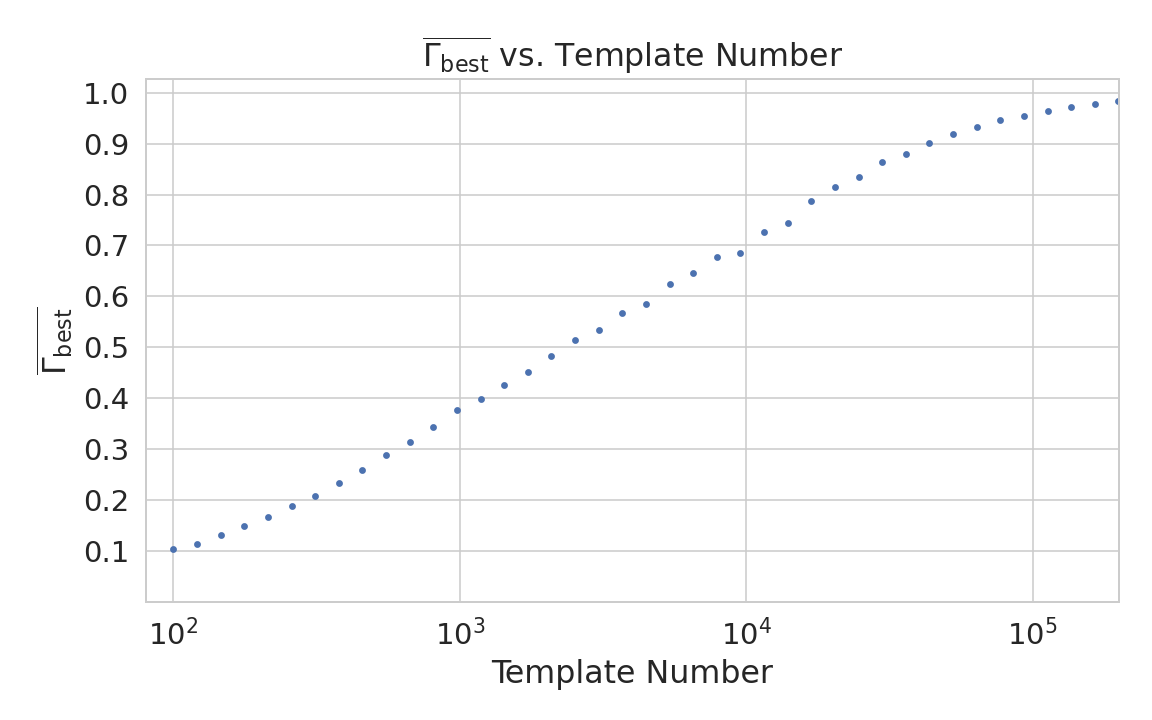
\includegraphics[width=0.69\textwidth]{figs/Chapter-4/230915_mean_match_vs_templates.png}
    \caption{The mean match of the matched filter template bank to a test set of randomly parameterized signals as a function of the number of templates. The parameter space includes pitch angles from $85.5-88.5^\circ$ and energies from $18575-18580$~eV.}
    \label{fig:match_vs_template_number}
\end{figure}

In this work we elected to evaluate the detection efficiency of a template bank where $\overline{\Gamma_\mathrm{best}}=0.95$. The number of templates required to achieve this value of mean match was determined by Monte-Carlo studies using template banks of different sizes, which were obtained by decimating the regularly spaced dataset (see Section \ref{sec:datasets}) with series of integer factors. The randomly parameterized signals were used as test signals to calculate the mean match of the template bank by evaluating 
\begin{equation}
    \overline{\Gamma_\mathrm{best}}=\frac{1}{N_s}\sum_{l=1}^{N_s}{\frac{\mathcal{T}_\mathrm{best}}{\mathcal{T}_l}},
\end{equation}
where $N_s$ is the number of test signals and $\mathcal{T}_l$ is the ideal matched filter score for test signal $l$, which is obtained if there is perfect match between signal and template. 

The results of these calculations are summarized by Figure \ref{fig:match_vs_template_number}, which shows $\overline{\Gamma_\mathrm{best}}$ as a function of the number of templates ($N_t$). The linear trend of $\overline{\Gamma_\mathrm{best}}$ as a function of the logarithm of $N_t$ indicates that match scales exponentially with the size of the template bank, although this trend breaks down at large $N_t$ when match begins to saturate close to unity. Using linear interpolation between the data points, we identify $\approx10^5$ as the number of templates consistent with $\overline{\Gamma_\mathrm{best}}=0.95$.

\subsubsection{CNN Training and Data Augmentation}
The random dataset is split in half to create distinct training and test datasets for training the model. A randomly selected 20\% of the training data is isolated for use as a validation set during the training loop. The size of the training, validation, and test datasets are tripled by appending two additional copies of the data to increase the sample size of the dataset after data augmentation. A different sample of noise is added to the simulation data during the training loop, which prevents the model from overtraining on noise features. The training and test datasets contain an equal split between signal and noise data, which are randomly shuffled after each training epoch.

The Locust simulation data was augmented to make the datasets more representative of actual experiment data. As the signals are loaded for training a unique random phase shift is applied. Since the simulations are generated using the same initial axial position and cyclotron orbit phase, the randomization is an attempt to prevent overtraining on these features. During each training epoch the data is randomly shuffled and split into batches of 2500 signals. Each batch of signals is then circularly shifted by a random number of frequency bins to simulate a kinetic energy shift from $-75$ to $20$~eV, which imitates a dataset with a larger energy range. Next, a sample of cWGN, consistent with 10~K Nyquist-Johnson noise, is generated and added to the signal, which prevents overtraining on noise features. As a final step, the data is renormalized by the standard deviation of the noise so that the range of values in the data is close to $[-1,1]$, which ensures well-behaved back-propagation.

\begin{figure}[htbp]
    \centering
    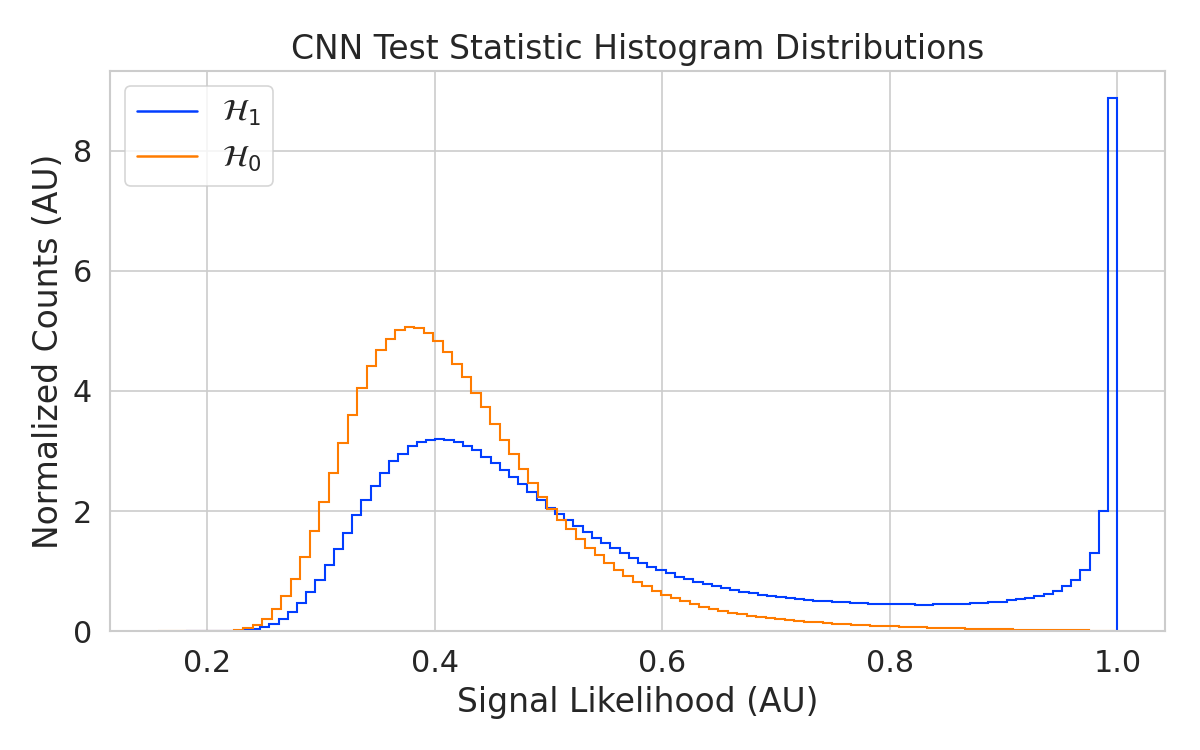
\includegraphics[width=0.69\textwidth]{figs/Chapter-4/230831_cnn_test_stat_hist.png}
    \caption{Histograms of the trained CNN model output from the test dataset. The blue histogram shows the model outputs for signal data. The oddly shaped peak near the end is the result of the softmax function mapping the long tail of the raw output distribution to the range $[0,1]$. }
    \label{fig:cnn_histogram}
\end{figure}

The Binary Cross-entropy loss function is used to compute the loss for each batch of data, and the model weights are updated using the ADAM optimizer with a learning rate of $5\times10^{-3}$. After each training epoch, the loss and classification accuracy of the validation dataset are computed to monitor for overtraining. It was noticed that because of the relatively high noise power and the fact that a new sample of noise was used for each batch, it was nearly impossible to over-train the model. Typically, the loss and classification accuracy of the model converged after a few hundred training epochs, but the training loop was extended to 3000 epochs to attempt to achieve the best possible performance. The training procedure generally took about 24~hrs using a single NVIDIA V100 Graphics Processing Unit (GPU) \cite{v100}.

After training the model, it was used classify the test dataset and generate histograms of the model outputs for both classes of data. The data augmentation procedure for the evaluation of the test data mirrors the training procedure without the validation split. Since a random circular shift and a new sample of WGN is added to each batch, the testing evaluation loop is run for 100 epochs to get a representative sample of noise and circular shifts. The model outputs are passed through a softmax activation and then combined into histograms (see Figure \ref{fig:cnn_histogram}).

\subsection{Results and Discussion}
\label{sec:results}

\subsubsection{Trigger Classification Performance}

\begin{figure}[htbp]
    \centering
    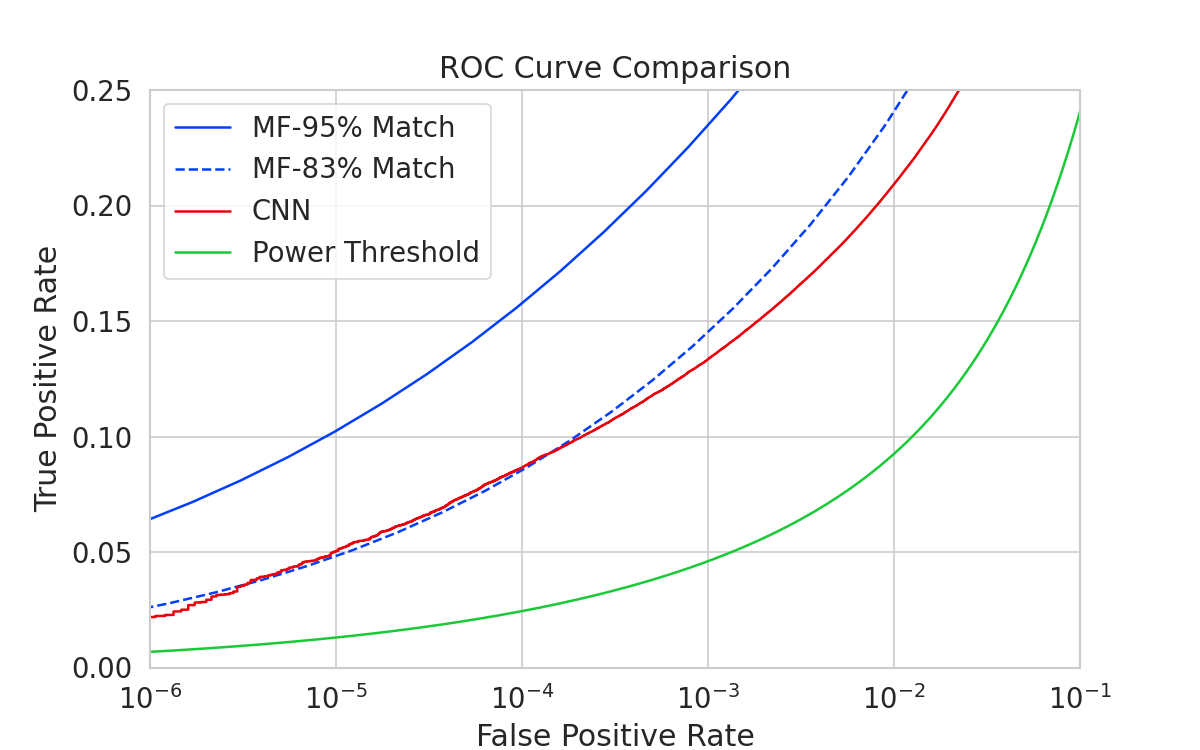
\includegraphics[width=0.7\textwidth]{figs/Chapter-4/230927_nn_roc_vs_mf_vs_fft.png}
    \caption{ROC curves describing the true positive rate (detection efficiency) for the three signal classification algorithms examined in this paper. The matched filter and power threshold curves are computed analytically using the distribution functions introduced in Section \ref{sec:classifiers}, and the CNN curve is computed numerically using the classification results on the test dataset. The percent match indicated in the legend refers to the value of $\overline{\Gamma_\mathrm{best}}$ for the template bank.
    }
    \label{fig:roc_compare}
\end{figure}
The detection performance of the signal classifiers can be compared by computing the receiver operating characteristic (ROC) curves (see Figure \ref{fig:roc_compare}).
A single ROC curve is obtained for the matched filter and power threshold classifiers by averaging over the distributions for individual CRES signals as described in Section \ref{sec:ensemble_average}. ROC curves are calculated for the matched filter using template banks of two different sizes corresponding to mean matches of 95\% and 83\%. The ROC curve describing the CNN is obtained numerically from the histograms of the model outputs for each signal class.

The true positive rates of the signal classifiers are equivalent to detection efficiency, and one sees that for the population of signals with pitch angles $<88.5^\circ$ the power threshold has a consistently lower detection efficiency than the CNN and the matched filter. This result might have been predicted from the visualization of signal spectra in Figure \ref{fig:signal_post_bf_example}, where it can be seen that a noise peak and a signal peak cannot be distinguished with high-confidence at small pitch angles. The CNN offers a significant and consistent increase in detection efficiency over the power threshold approach. 

If one compares the CNN to the matched filter, it can be seen that the performance of the tested network is roughly equivalent to a matched filter detector with a mean match of about 83\%, which uses approximately $2\times10^4$ matched filter templates. The overall best detection efficiency is achieved by the matched filter classifier if a large enough template bank is used. The plot displays the ROC curve for a matched filter template bank with 95\% mean match, which is achieved with approximately $10^5$ templates. Since the matched filter is known to be statistically optimal for detecting a known signal in WGN, it is unsurprising that this algorithm has the highest detection efficiency.

An important difference between the matched filter and CNN algorithms is that the CNN relies upon convolutions as its fundamental calculation mechanism, whereas our implementation of a matched filter utilizes an inner product. Since convolution is a translation invariant operation, the detection performance of CNN can be extended to a wider range of CRES event kinetic energies with less cost than the matched filter, a feature that is exploited during the CNN training by including circular translations of the CRES frequency spectra in the training loop. Increasing the range of detectable kinetic energies with a matched filter requires a proportional increase in the number of templates, which directly translates into increased computational and hardware costs. From a practical perspective, the detection algorithm is always limited by the available computational hardware, so estimating the relative costs is a key factor in determining their feasibility. A more detailed analysis of the relative costs of each of the detection algorithms is performed below.


\subsubsection{Computational Cost and Hardware Requirements}
\label{sec:dis-comp-cost}

The trade-off between better detection efficiency and computational cost is common to many signal detection problems and the FSCD is no exception. Computational costs can be related to actual hardware costs by calculating the theoretical amount of computer hardware required to implement the signal classifiers for real-time detection. The approach taken here utilizes order of magnitude estimates of the theoretical peak performance values for currently available GPUs as a metric. This approach underestimates the amount of required hardware, since it is unlikely that any CRES detection algorithm could reach the theoretical peak performance of the hardware. 

Since the signal detection algorithms are designed to work using beamformed frequency spectra, the computational cost of beamforming combined with a fast Fourier transform (FFT) is constant for all classifiers. The beamforming grid is assumed to contain $N_\mathrm{bf}$ beamforming positions, each of which will produce a frequency spectrum containing $N_\mathrm{bin}$ after the FFT. 

Considering the power threshold classifier, this results in $N_\mathrm{bin}N_\mathrm{b}$ frequency bins that must be checked every $N_\mathrm{bin}/f_\mathrm{s}$ seconds. The 20~cm diameter FSCD array requires $N_\mathrm{bf}\approx O(10^2)$ for sufficient coverage and has a sampling frequency $f_\mathrm{s}=200$~MHz with a Fourier analysis window of $N_\mathrm{bin}=8192$ samples. Therefore the power threshold requires approximately $O(10^{10})$~FLOPS to check in real-time with these parameters.

Current generations of GPUs have peak theoretical performances in the range of $O(10^{13})-O(10^{14})$~FLOPS \cite{h100}, dependent on the required floating-point precision of the computation. Therefore, the entire computational needs of a real-time triggering system using a power threshold classifier, including digital beamforming and generation of the STFT, could be met by a single high-end GPU or a small number of less powerful GPUs. Since triggering is only one step of the full real-time signal reconstruction approach, limiting the computational cost of this stage is ideal. However, the power threshold classifier does not provided sufficient detection efficiency across the entire range of possible signals, which is the primary motivation for exploring more complicated triggering solutions. 

As discussed, the computational cost of the matched filter approach requires counting the number of templates that must be checked for each frequency spectra produced by the STFT. Computing the matched filter scores requires $O(N_\mathrm{bf}N_\mathrm{t}N_\mathrm{bin})$ operations, since for each of the beamforming positions one must multiply $N_\mathrm{t}$ templates with a data vector that has length $N_\mathrm{bin}$. The computation must be performed in a time less-than or equal to $N_\mathrm{bin}/f_\mathrm{s}$ to keep up with the data generation rate. A 5~eV range of kinetic energies required $10^4$ to $10^5$ templates in order for the matched filter to exceed the performance of the CNN. The number of templates is expected to scale linearly with the total kinetic energy range of interest, therefore, $10^5$ to $10^6$ matched filter templates would be expected for the nominal 50~eV analysis window of the FSCD. Considering this, the estimated computational cost to implement a matched filter in a FSCD-scale experiment is between $O(10^{15})$ to $O(10^{16})$~FLOPS, which is $O(10^2)$ to $O(10^3)$ high-end GPUs .

The computational cost of the CNN can be estimated by simply summing the computational costs of the convolutions and matrix multiplications specified by the network architecture shown in Table \ref{tab:cnn_model_params}. Each convolutional layer consists of $N_\mathrm{in}N_\mathrm{out}N_\mathrm{kernel}L_\mathrm{input}$ floating-point operations, where $N_\mathrm{in}$ is the number of input channels, $N_\mathrm{out}$ is the number of output channels, $N_\mathrm{kernel}$ is the size of the convolutional kernel, and $L_\mathrm{input}$ is the length of the input vector, and the fully connected layers each contribute $N_\mathrm{in}N_\mathrm{out}$ operations. Summing all the neural network layers it is estimated that the CNN requires $O(10^6)$ floating point operations to evaluate each frequency spectra; therefore, the total computational cost of the CNN trigger is value multiplied by the number of beamforming positions per the data acquisition time, which is $O(10^{13})$~FLOPS or $O(10^0)$ GPUs.

Compared with the matched filter template bank approach the CNN requires $O(100)$ to $O(1000)$ fewer GPUs to implement, dependent on the exact number of templates used in the template bank. The 50~eV kinetic energy range is motivated by the application of these detection algorithms to an FSCD-like neutrino mass measurement experiment. However, if a significantly larger range of kinetic energies is required, a CNN may be the preferred detection approach despite the lower mean detection efficiency due to computational cost considerations.


Additional experiments with larger CNNs, generated by increasing the depth and width of the neural network, were performed. It was observed that these changes provided minimal ($\lesssim 1\%$) improvement in the classification accuracy of the model. A potential reason for this could be the sparse nature of the signals in the frequency domain and the low SNR, which makes for a challenging dataset to learn from. Future work might investigate modifications to the neural network architecture such as sparse convolutions, which may improve the classification accuracy of the model or further reduce the computational costs of this approach. Alternatively, more complicated CNN architectures such as a ResNet \cite{resnet, vgg} or VGG model may provide improved classification performance over a basic CNN. An additional promising area of investigation are recurrent neural networks, which may be able to exploit the time-ordered features of the STFT for more accurate signal detection if the electron signals last for multiple Fourier transform windows.

The estimate of the computational costs of the matched filter is somewhat naive if one notices that the majority of the values that make up a noise-free CRES frequency spectrum are zero (see Figure \ref{fig:signal_post_bf_example}). Therefore, the majority of operations in the matched filter inner product are unnecessary, and one could instead evaluate the matched filter inner product using only the $\lesssim10$ frequency peaks that make up the CRES signal. This optimization reduces the number of operations required to check each template by a factor of $O(100)$ to $O(1000)$, which brings the estimated computational cost of the matched filter in line with the CNN. Although this level of sparsity results in a multiplication with very low arithmetic complexity, the resulting sparse matched filter algorithm is still likely to be constrained by memory access speed rather than compute speed. Ultimately, the comparison of the relative computational and hardware costs between the matched filter and CNN will depend on the efficiency of the software implementation and hardware support for neural network and sparse matrix calculations, which will need to be determined using real-world benchmarks.



\subsection{Conclusion}
\label{sec:conclusion}

Increasing the detection efficiency and overall event rate represents a key developmental path towards new scientific results and broader applications of the CRES technique. It is what motivates both the antenna array detection approach and the development of real-time signal reconstruction algorithms. The work presented here demonstrates that gains in detection efficiency are achievable by utilizing triggering algorithms that account for the specific shape of CRES signals in the detector. These algorithms emphasize the need for accurate and fast methods for CRES simulation, since they directly contribute to the success of matched filter methods by providing a way to generate expected signal templates and also serve as a source of training data for machine learning approaches. 

The down-side of more advanced approaches to signal detection and reconstruction is oftentimes the increase in computational resources required to implement them. However, it was shown that a CNN of minimal size was able to significantly improve detection performance above the baseline power threshold trigger algorithm with a theoretical computational cost of only $O(1)$ high-end GPU. This algorithm improves on detection performance while requiring at least a factor $O(10^2)$ less in computer relative to a matched filter template bank, which would be the classical approach to signal detection in Gaussian noise. Future work that obtains real-life benchmarks of the CNN and matched filter algorithms are required to support these conclusions, but this study has indicated that a real-time signal detection algorithm for an antenna array CRES experiment is computationally feasible without an extraordinary increase in resources.

It is worth emphasizing that, while this real-time signal detection algorithm has been developed specifically for the FSCD experiment, which uses a 60-channel array of antennas, this approach allows one to combine the signals from an array with an arbitrary number of receiving elements. Therefore, this general procedure could be implemented to perform signal reconstruction with close to optimal efficiency, especially if a matched filter classifier is used, for significantly larger antenna-based CRES experiments.

While this work has focused on the real-time detection of CRES signals from antenna arrays, these same signal classifiers could be used in CRES experiments utilizing different detector technologies, since the same principles of signal detection will apply. For example, previous CRES measurements by the Project 8 collaboration that utilized a waveguide gas cell, could in principle increase detection efficiency by employing a matched filter or neural network classifier to identify trapped electrons with pitch angles that are too small to be detected by the power threshold approach. Furthermore, alternative CRES detector technologies such as resonant cavities \cite{p8snowmass2022} could also see similar improvements in detection efficiency, which is of crucial importance to future efforts by the Project 8 collaboration to utilize CRES to measure the neutrino mass.


% !TEX root = ../YourName-Dissertation.tex

\chapter{Antenna and Antenna Measurement System Development for the Project 8 Experiment}

\section{Introduction}

The FSCD and antenna array CRES represent an innovative approach to beta-decay spectroscopy. While much can be learned from simulations about the systematics of CRES with antenna arrays, laboratory measurements and demonstrations provide critical inputs to sensitivity and simulation models as well as provide a means for calibration and commissioning of the experiment. Therefore, a robust program of antenna and antenna measurement hardware development is important to the success of the FSCD and the development of antenna array CRES more broadly.

In this chapter we summarize the development of an antenna measurement system at Penn State to implement and test the techniques of antenna array CRES on the bench-top, in order to support the efforts of the Project 8 collaboration. In Section \ref{sec:chap4-ant-meas} we provide an introduction to some fundamental parameters and concepts related to antenna measurements as well as an overview of the Penn State antenna measurement system hardware. In Section \ref{sec:SYNCA} we include the manuscript of a paper \cite{p8synca} which details the design and characterization of a specialized antenna developed to mimic the electric fields emitted by an electron in a CRES experiment. This antenna, called the Synthetic Cyclotron Antenna (SYNCA), is intended as a calibration tool for antenna arrays developed for CRES measurements. Lastly, in Section \ref{sec:chap5-fscd-array-measurements} we summarize a set of prototype FSCD antenna array measurements with the SYNCA \cite{p8jugaad}, which we use to validate the simulated performance of the antenna array and estimate systematic errors associated with the antenna array.

\section{Antenna Measurements for CRES experiments}
\label{sec:chap4-ant-meas}

\subsection{Antenna Parameters}
\label{sec:ant-meas-fun}

Antenna characterization measurements are intended to validate simulations of the antenna array performance, which ultimately informs the neutrino mass sensitivity of the experiment. In this section, I shall summarize a few fundamental concepts relating to antennas and antenna measurement, before introducing how Project 8 uses antenna measurement for the development of antenna array CRES.

\subsubsection{Radiation Patterns}

\begin{figure}[htbp]
    \centering
    \begin{subfigure}[b]{0.48\textwidth}
        \centering
        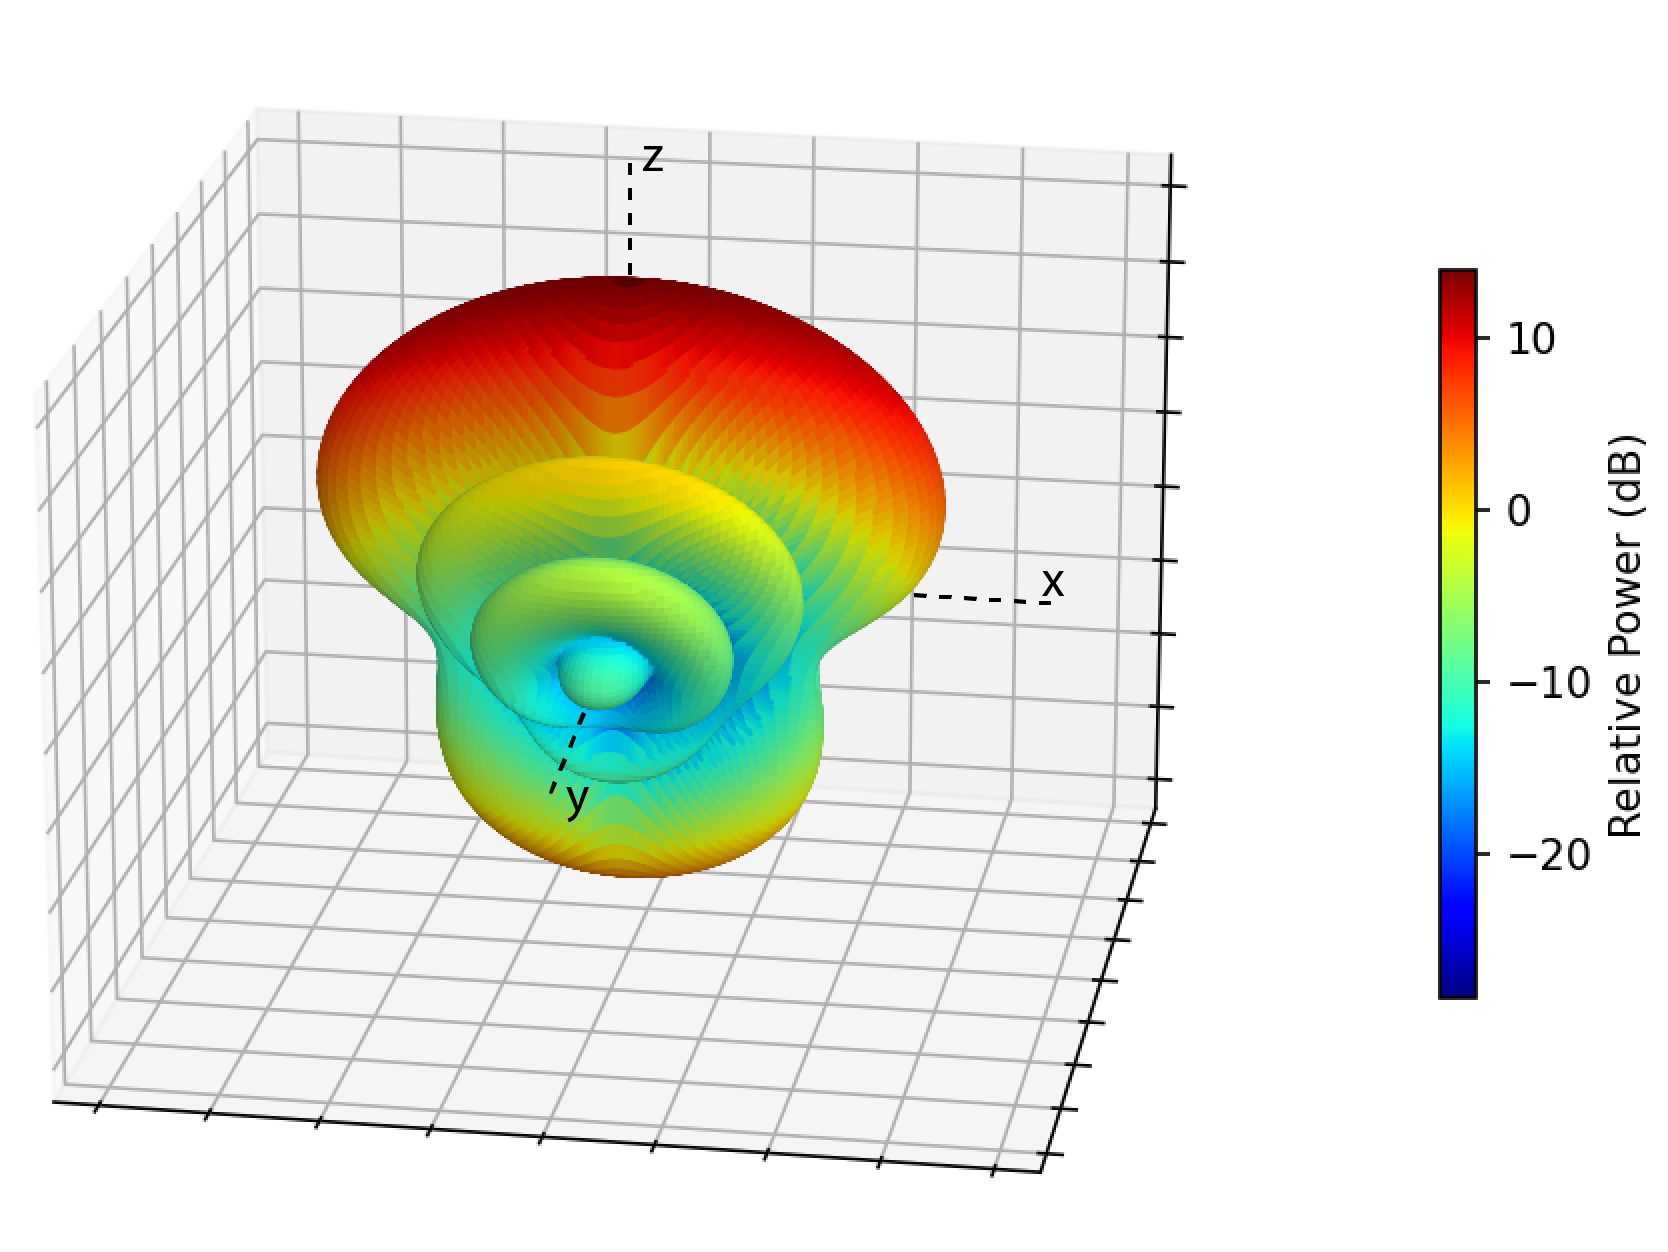
\includegraphics[width=1\textwidth]{figs/Chapter-5/230419_example_radiation_pattern2.png}
        \caption{\label{fig:rad-pattern-ex1}}
    \end{subfigure}
    \hfill
    \begin{subfigure}[b]{0.48\textwidth}
        \centering
        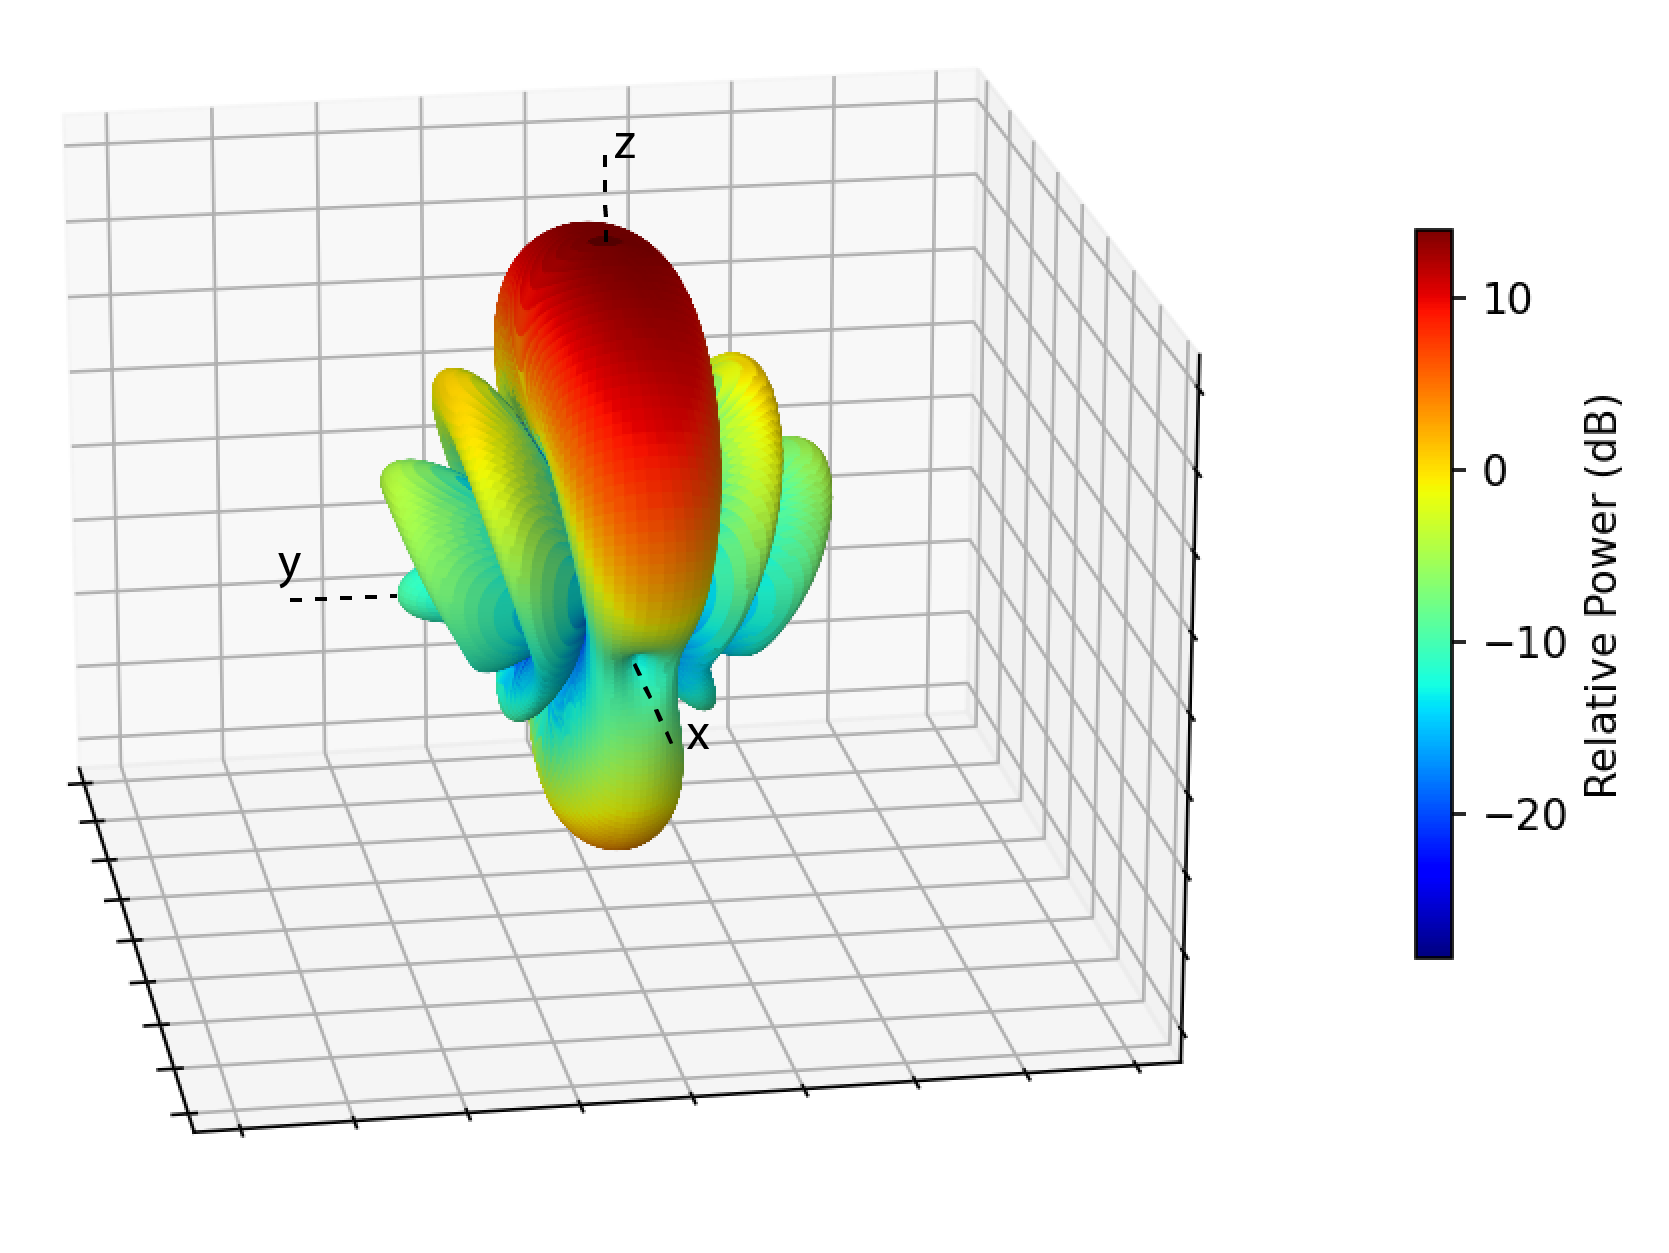
\includegraphics[width=1\textwidth]{figs/Chapter-5/230419_example_radiation_pattern.png}
        \caption{\label{fig:rad-pattern-ex2}}
    \end{subfigure}
    \hfill
    \caption{An example radiation pattern generated using HFSS simulations. The color and radial distance of the surface from the origin indicate the relative magnitude of radiation power emitted by the antenna in that direction. The primary goal of most antenna measurements is typically to measure the antenna pattern, which is used to derive many useful antenna performance parameters.}
    \qquad
    \label{fig:rad-pattern-examples}
\end{figure}

Antennas are conductive structures designed to carry alternating electric currents in order to transmit energy in the form of electro-magnetic (EM) waves \cite{balanis2015antenna}. Perhaps the most fundamental way to characterize an antenna, is to map out the radiated power density as a function of position, which is called the radiation pattern (see Figure \ref{fig:rad-pattern-examples}). We find the radiation power density by calculating the time-averaged Poynting vector for all positions surrounding the antenna, which in equation form is
\begin{equation}
    \mathbf{W}(x,y,z) = \left<\mathbf{E}(x,y,z,t)\times\mathbf{H}^\ast(x,y,z,t)\right>_t,
\end{equation}
where $\mathbf{E}(x,y,z,t)$ and $\mathbf{H}(x,y,z,t)$ are the time-dependent electric and magnetic fields produced by the antenna \cite{jackson_classical_1999}. The radiation power density has units of $\mathrm{W}/\mathrm{m}^2$ and is more typically called the energy flux density in physics applications, since it is a measure of the amount of energy passing through a unit area over time. 

Because the radiation power density is a measure of power per unit area, its value in a particular direction will depend on the distance from the antenna at which we are measuring. This is undesirable for practical applications A related quantity, which is distance independent, is the energy flux per unit solid angle or radiation intensity, which is computed directly from the radition power density by multiplying by the squared distance from the antenna. Specifically,
\begin{equation}
    U = r^2W(x,y,z),
\end{equation}
where $r$ is the distance from the antenna to the field measurement point. The radiation intensity is typically defined in regions where the Poynting vector consists only of a radial component where it is safe to treat as a scalar quantity. 

\subsubsection{Directivity and Gain}
Since the radiation intensity is a measure of average power per unit solid angle, it is independent of distance and more useful as feature for antenna measurement. However, most antenna measurements are performed in terms of the directly related directivity and gain quantities. Directivity is defined as the ratio between the radiation intensity at particular point on the radiation pattern to the average radiation intensity computed over all solid angles \cite{balanis2015antenna}.
The equation that relates the radiation intensity to directivity is
\begin{equation}
    D = \frac{U}{U_0}=\frac{4\pi U}{P_\textrm{rad}},
\end{equation}
where $U_0$ is the average radiation intensity over all solid angles, which simply the total radiated power ($P_\textrm{rad}$) divided by $4\pi$. Closely related to directivity is concept of gain, which accounts for energy losses that occur inside then antenna when attempting to transmit or receive a signal. The antenna gain is given by 
\begin{equation}
    G=\frac{4\pi U}{P_\mathrm{in}},
\end{equation}
where $P_\mathrm{in}$ is the total power delivered to the antenna. Gain can be thought of as the ratio of the antenna's radiation intensity to that of a hypothetical isotropic, lossless radiator. The maximum values of gain and directivity exhibited by the main lobe of the antenna pattern as well as the ratio between the gain of the main lobe and any side-lobes are important figures of merit used to evaluate antenna designs. 

\begin{figure}[htbp]
    \centering
    \includegraphics[width=0.7\textwidth]{figs/Chapter-5/230421_field_regions.png}
    \caption{An illustration of the three field regions important for the analysis of an antenna system. Very close to the antenna the electric fields are primarily reactive so there is no radiation. If a receiving antenna were placed in this region most of the energy would be reflected back to the transmitter. Outside of the reactive near-field is the radiative near field. At these distances the antenna does radiate, but the radiation pattern is not well-defined since it changes based on the distance of the receiving antenna. It is only in the far-field region where the radiation pattern becomes constant as a function of distance, which is where the majority of antenna engineering is assumed to take place. The antenna arrays developed by Project 8 for CRES measurements operate in the radiative near-field due to the importance of limiting power loss from free-space propagation, which complicates the design of the antenna system.}
    \label{fig:field-regions}
\end{figure}

\subsubsection{Far-field and Near-field}
Radiation patterns are only well-defined in regions where the shape of the radiation pattern is independent of distance. The region where this approximation is valid is called the "far-field", and in this region we can treat the EM fields from the antenna as spherical plane waves. A rule of thumb for antennas is that the far-field approximation is valid when the condition
\begin{equation}
    R > \frac{2l^2}{\lambda}
\end{equation}
is met. In this expression, $R$ is the distance from the antenna, $l$ is the largest characteristic dimension of the antenna, and $\lambda$ is the wavelength of the radiation (see Figure \ref{fig:field-regions}). 

The region very close to the antenna is called the reactive near-field, because in this region the reactive component of the EM field is dominant. Unlike radiative electric fields, the reactive electric and magnetic fields are out of phase from each other by $90^\circ$, since they are the result of electrostatic and magnetostatic effects coming from the self-capacitance and self-inductance of the antenna. The reactive fields are unable to transfer energy a significant distance from the antenna and are thus completely negligible for most antenna applications. The limit of the reactive near-field for an electrically-large antenna is typically taken to be
\begin{equation}
    R<0.62\sqrt{l^3/\lambda}.
\end{equation}
The unique application of antennas by Project 8 is somewhat limited by reactive near-field effects in the form of a maximum radial position for electrons inside the uniform cylindrical antenna array. If electrons are too close to the edge of the array than reactive near-field effects leads to a large reduction in the received power and consequently detection efficiency. This leads to a significant volume inside of the antenna array that is unsuitable for CRES lowering the volumetric efficiency of the antenna array CRES technique relative to a cavity experiment.

In between the reactive near-field and the far-field is the radiative near-field region. In this region the fields are primarily radiative, however we are still too close to the antenna for the spherical plane wave approximation to apply. Therefore, interference effects between EM waves emitted from different points on the antenna occur causing the shape of the radiation pattern to change as a function of distance from the antenna. If we evaluate the far-field distance limit for the FSCD one finds an estimated far-field distance of 43~cm, which is a factor of four larger than the radius of the antenna array designed for the experiment. Consequently, we expect near-field effects to influence the performance of the antenna array highlighting the importance of calibration and characterization measurements.

\subsubsection{Polarization}
The polarization of an EM wave defines the spatial orientation of the electric field oscillations in the plane perpendicular to the direction of the propagation, and is defined in terms of orthogonal polarization components. In our application, one analyzes the properties of radiation propagating along the radial ($\hat{r}$) direction away from the antenna, which implies that the electric fields can be described as a linear combination of orthogonal polarization components
\begin{equation}
    \mathbf{E}_\mathrm{tot}=E_x\hat{x}+E_y\hat{y}+E_z\hat{z},
\end{equation}
in Cartesian coordinates, or
\begin{equation}
    \mathbf{E}_\mathrm{tot}=E_\theta\hat{\theta}+E_\phi\hat{\phi},
\end{equation}
in spherical coordinates. 

In general, one defines partial radiation patterns, directivities, and gains so that the performance of the antenna for the desired polarization can be analyzed. The radiation pattern defined in terms of partial patterns is
\begin{equation}
    U_\mathrm{tot}=U_\phi + U_\theta,
\end{equation}
where $U_\phi$ and $U_\theta$ are the radiation intensities in a particular direction for the respective polarization components. Similarly, a quantity such as gain can be written in terms of partial gains,
\begin{equation}
    G_\mathrm{tot}=G_\phi+G_\theta=\frac{2\pi U_\phi}{P_\mathrm{in}}+\frac{2\pi U_\theta}{P_\mathrm{in}}.
\end{equation}

If we view an electron performing a circular orbit in the XY-plane from the side, that is, along the X or Y axes, then we would observe the electron to be performing a linear oscillation perpendicular to the viewing axis. From this intuitive picture, we can predict that the primary polarization of electric fields from CRES events to be linearly polarized in the $\hat\phi$ direction when viewed with an antenna positioned in the XY-plane.

\subsubsection{Antenna Factor and Effective Aperture}
\label{sec:ant-factor}
A useful way to characterize the performance of an antenna is to measure the electric field magnitude required to produce a signal with an amplitude of one volt in the antenna terminals. This ratio between the magnitude of the incoming electric field and the magnitude of the signal produced by the antenna is called the antenna factor, which is written as
\begin{equation}
    A_\mathrm{F} = \frac{|\mathbf{E}_\mathrm{in}|}{V_\mathrm{ant}},
    \label{eq:antenna-factor}
\end{equation}
where $A_\mathrm{F}$ is the antenna factor, $E_\mathrm{in}$ is the incoming electric field, and $V_\mathrm{ant}$ is the magnitude of the voltage produced by the antenna.

The antenna factor can be expressed in terms of the antenna's gain through a related quantity called the effective aperture. The effective aperture defines for a given incident radiation power density ($\mathrm{W}/\mathrm{m}^2$) the power that is received by the antenna. Therefore, the effective aperture gives the equivalent area of the antenna,
\begin{equation}
    A_\mathrm{eff}=\frac{P_\mathrm{rec}}{P_\mathrm{in}}=\frac{\lambda^2}{4\pi}G,
\end{equation}
where the received power is $P_r$ and the total incoming power is $P_\mathrm{in}$.

If we express the incident power in terms of the magnitude of the Poynting vector, then
\begin{equation}
    |\mathbf{S}_\mathrm{in}|=|\mathbf{E}_\mathrm{in}|^2/\eta_0,
\end{equation}
where $\eta_0$ is the impedance of free-space, which relates the magnitudes of the electric and magnetic fields in a vacuum, and is defined by
\begin{equation}
    \eta_0 = \frac{|\mathbf{E}|}{|\mathbf{H}|} = \sqrt{\frac{\epsilon_0}{\mu_0}}.
\end{equation}
The total received power by the antenna can therefore be expressed as
\begin{equation}
    P_\mathrm{rec}=|\mathbf{S}_\mathrm{in}|A_\mathrm{eff}=|\mathbf{S}_\mathrm{in}|\frac{\lambda^2}{4\pi}G=\frac{|\mathbf{E}_\mathrm{in}|^2\lambda^2G}{4\pi\eta_0}.
    \label{eq:power-rec-1}
\end{equation}

To relate this to the antenna factor recall that we can relate the voltage produced by the antenna to the received power with
\begin{equation}
    P_\mathrm{rec}=\frac{V_\mathrm{ant}^2}{Z}=\frac{|\mathbf{E}_\mathrm{in}|^2}{A_\mathrm{F}^2Z},
    \label{eq:power-rec-2}
\end{equation}
where $Z$ is the system impedance. Setting Equations \ref{eq:power-rec-1} and \ref{eq:power-rec-2} equal to each other, we obtain the following expression for antenna factor in terms of gain
\begin{equation}
    A_\mathrm{F} = \sqrt{\frac{4\pi\eta_0}{ZG\lambda^2}}=\frac{9.73}{\lambda\sqrt{G}}.
    \label{eq:ant-factor}
\end{equation}
The second expression in Equation \ref{eq:ant-factor} is obtained by evaluating the constant terms assuming a system impedance of 50~$\Omega$.

We have gone through the effort of expressing the antenna factor in terms of gain to highlight that the majority of antenna parameters that we care to measure for a CRES experiment can be obtained from the radiation or gain pattern of the antenna. The antenna factor is a particularly important parameter for CRES measurements due to it's relevance to antenna array simulations with the Locust software \cite{p8locustpaper, nb_thesis}. Specifically, Locust simulates the trajectory of an electron in a magnetic trap by running the Kassiopeia software package \cite{kassiopeia} and then uses the Li\'{e}nard-Wiechert equations \cite{lw_potential_1, lw_potential_2} to calculate the electric fields that are incident on the antenna. 

To compute the response of the antenna to the electric field, Locust relies upon linear time-invariant system theory \cite{lti_theory_wiki}, which computes the response of the antenna (i.e. the voltage time series generated by the antenna) using a convolution between the electric field time-series and the antenna impulse response. This approach is necessary for correctly modeling the antenna response to the electric field due to the broadband and non-stationary nature of the electric fields from CRES events. Since antenna measurements take place under steady-state conditions, parameters such as the radiation pattern, gain, and antenna factor are defined in the frequency domain. However, by performing an inverse Fourier transform on the antenna factor we can obtain the antenna impulse response, which allows us to simulate CRES events in the antenna array demonstrator experiment. 

\subsection{Antenna Measurement Fundamentals}
\subsubsection{Friis Transmission Equation}

The antenna factor, sometimes called the antenna transfer function, is used to model how the antenna will respond to electric fields emitted from a CRES event. Therefore, being able to measure the antenna transfer function of the antenna array is a key step in the commissioning and calibration phases of an antenna array CRES experiment. A common approach to antenna characterization is to perform a two antenna transmit-receive measurement where an antenna with a known gain is used to characterize the unknown gain of the antenna under test (see Figure \ref{fig:friis-meas}). 
\begin{figure}[htbp]
    \centering
    \includegraphics[width=0.6\textwidth]{figs/Chapter-5/230409_friis_figure.png}
    \caption{An illustration of the Friis measurement technique commonly used for antenna characterization measurements.}
    \label{fig:friis-meas}
\end{figure}

To analyze this two antenna setup we seek to calculate the amount of power from the transmitting antenna that we will detect with the receiving antenna. Using our understanding of antenna gain, we can calculate the power density transmitted by an antenna in a direction $(\theta_t,\phi_t)$ at frequency $f$ and distance $R$, which is given by
\begin{equation}
    w_t = \frac{P_t}{4\pi R^2}G_t(\theta_t,\phi_t,f).
\end{equation}
Here, $P_t$ is the total power delivered to the transmitting antenna and $G_t(\theta_t,\phi_t,f)$ is the value of the transmitting antenna gain. The power density is the power per unit area, so to calculate the total power delivered to the receiving antenna we multiply the transmitted power density by the effective area of the receiving antenna,
\begin{equation}
    P_r = w_tA_{eff,r}=P_t\frac{G_t(\theta_t,\phi_t,f)G_r(\theta_r,\phi_r,f)c^2}{(4\pi Rf)^2},
    \label{eq:friis-eqn}
\end{equation}
where $G_r(\theta_r,\phi_r,f)$ is the gain of the receiving antenna. Equation \ref{eq:friis-eqn} is called the Friis transmission equation \cite{friis_paper,friis_wiki}, which is of fundamental importance for antenna measurements, since it allows one to measure the gain of an unknown antenna by measuring the power received from an antenna with a known gain pattern. Alternatively, if no antenna with a known gain pattern is available, two identical antennas with unknown gain patterns can be used.

\subsubsection{S-Parameters and Network Analyzers}

Instead of directly measuring the power received by the antenna under test, it is more common to measure the ratio of the received power to the transmitted power,
\begin{equation}
    \frac{P_r}{P_t} = \frac{G_t(\theta_t,\phi_t,f)G_r(\theta_r,\phi_r,f)c^2}{(4\pi Rf)^2}.
\end{equation}
This power ratio can be easily measured using a vector network analyzer (VNA), which automates a significant fraction of the measurement process. Network analyzers are used to measure the scattering or S-parameters of a multi-port RF device \cite{pozar}, which describes how waves are scattered between the device ports. The antenna measurements we have been considering can be modeled as a two-port microwave device that we can characterize by measuring how incident voltage waves are transmitted or reflected (see Figure \ref{fig:2port-scattering}).
\begin{figure}[htbp]
    \centering
    \includegraphics[width=0.5\textwidth]{figs/Chapter-5/230429_2port_scattering_figure.png}
    \caption{Illustration of a two-port S-parameter measurement setup. S-parameters characterize how incoming waves of voltage or power scatter of of the RF device under test. This allows you to measure important properties of the device. In particular, we can use this framework to model a two antenna radiation pattern measurement, which we can then automate using a VNA. }
    \label{fig:2port-scattering}
\end{figure}
We can write the scattered waves ($V_1^-$ and $V_2^-$) in terms of the incident ($V_1^+$ and $V_2^+$) waves using the scattering matrix
\begin{equation}
    \begin{pmatrix}
        V_1^-\\
        V_2^-
    \end{pmatrix} = 
    \begin{pmatrix}
        S_{11}&S_{12}\\
        S_{21}&S_{22}
    \end{pmatrix}
    \begin{pmatrix}
        V_1^+\\
        V_2^+
    \end{pmatrix},
\end{equation}
where the elements of the matrix are the device S-parameters. It is assumed that, when exciting the device from a particular port, that all other ports in the network are terminated at the system impedance. This ensures that the incident waves from other ports in the network are zero. Therefore, the S-parameters are the ratios between the scattered and incident waves,
\begin{equation}
    S_{ij} = \frac{V_i^-}{V_j^+}.
\end{equation}
Alternatively, S-parameters can be defined as the ratio of the scattered and incident power, which is proportional to the ratio of the squared voltage waves. Returning to our antenna measurement setup, we see that measuring the ratio of the received to the transmitted power is equivalent to measuring the ratio of power being scattered from port 1 to port 2 in a RF network. Therefore, measuring an antenna's gain can be accomplished quite easily, by using a VNA to perform a two port $S_{21}$ measurement.

\subsubsection{Antenna Array Commissioning and Calibration Measurements}

Up to this point we have been discussing calibration and commissioning measurements as they apply to a single antenna. While these measurements play an important role in validating the radiation patterns of the individual array elements, the ultimate goal is to use a phased array of these antennas. Therefore, we must also consider antenna measurement techniques that apply to the whole array system.
\begin{figure}[htbp]
    \centering
    \begin{subfigure}[b]{0.4\textwidth}
        \centering
        \includegraphics[width=1\textwidth]{figs/Chapter-5/230409_beamform_array_meas.png}
        \caption{\label{fig:beam-array-meas}}
    \end{subfigure}
    \hfill
    \begin{subfigure}[b]{0.4\textwidth}
        \centering
        \includegraphics[width=1\textwidth]{figs/Chapter-5/230409_beamform_synth_array_meas.png}
        \caption{\label{fig:beam-synth-array-meas}}
    \end{subfigure}
    \hfill
    \caption{Two measurement approaches to characterizing an antenna array for CRES measurements. The full-array approach (a) requires a complete antenna array with all the associated hardware. The synthetic array approach (b) utilizes a single antenna and a set of rotation/translation stages to reposition the transmitter or the recieing antenna to synthesize the signals that would be received by the full-array. This approach reduces the cost and complexity of array measurements. A down-side of the synthetic array approach is that multi-channel effects such as reflections cannot be measured. Utilizing both the full-array and the synthetic array is a powerful way to quantify the impact of errors from the multi-channel array.}
    \qquad
    \label{fig:array-measurements}
\end{figure}

By measuring the gain of each individual array element we can predict the features of the signals received during a CRES event using the antenna factor (see Section \ref{sec:ant-factor}). However, unpredictable changes to the antenna performance can be introduced by the incorporation of the antennas into the circular array geometry, therefore, we employ both individual antenna and full-array measurements in the commissioning of the FSCD to account for these effects.

There are two main approaches to array measurements that could be used for characterization and calibration (see Figure \ref{fig:array-measurements}). One approach is to construct the complete array and use a omni-directional transmitting antenna to measure the power received by each channel in the antenna array. In Section \ref{sec:SYNCA} we describe the development of an omni-directional transmitter that also mimics the radiation phase characteristics of a CRES event, which is useful because the entire array can be tested without repositioning. Alternatively, a full antenna array can by synthesized by repeatedly moving and measuring a single array element. This approach is ideal for identifying if different channels in the antenna array are affecting each other through multi-path interference by comparing the measurement results of the synthetic array to the real array. 

\subsection{The Penn State Antenna Measurement System}
\label{sec:antenna_measurement_system}

The development of antenna array based CRES requires the capability to test and calibrate different antenna array designs to validate the performance of the as-built antenna array before and during the experiment. With these aims in mind we developed an antenna measurement system at Penn State specifically designed to mimic the characteristics of the antenna experiment designed for demonstration of the antenna array CRES technique by the Project 8 collaboration. 

The Penn State antenna measurement system utilizes a two antenna measurement configuration with a stationary reference antenna and a test antenna mounted on a set of motorized translation and rotation stages (see Figure \ref{fig:meas-sys-cartoon}). The antenna measurement system can be operated in two distinct modes, one focused on the characterization of the radiation patterns of prototype antennas and the other focused on the validation of data-acquisition (DAQ) and CRES signal reconstruction techniques to bridge the gap between real measurements and simulation. In both measurement configurations it is critical to isolate the antennas from the environment so that multi-path reflections do not negatively influence the measurement results. For this reason we surround the measurement volume with microwave absorber foam (AEMI AEC-1.5) \cite{absorber_foam} specifically designed to attenuate microwave radiation near the 26 GHz measurement range of the system.

\begin{figure}[htbp]
    \centering
    \includegraphics[width=0.5\textwidth]{figs/Chapter-5/230409_measurement_system_figure_cartoon.png}
    \caption{Illustration of the antenna measurement system developed for the Project 8 Collaboration. The reference and test antennas can be connected to different data acquisition configurations depending on the measurement goals The reference antenna is typically a standard horn antenna and the test antenna is mounted on a set of translation stages for positioning. Automated translation stages allows for relatively painless data-taking enabling synthetic antenna array measurements using only a single receiving antenna. Anechoic form designed to mitigate RF reflections surrounds the setup.}
    \label{fig:meas-sys-cartoon}
\end{figure}

In the first measurement configuration the reference antenna is typically a well-characterized horn antenna as pictured, since horn antennas have well-known and stable radiation patterns making them ideal as standard references. For characterization measurements, the test antenna represents the antenna-under-test whose pattern we wish to characterize. Mounting the test antenna on motorized rotation and translation stages allows us to automate the procedure significantly speeding up the radiation pattern measurement process. 

In the second measurement configuration one is interested in recreating the conditions of an antenna array CRES experiment as it concerns the antenna array and DAQ system. In this case, the reference antenna is a prototype FSCD antenna, which will be used to construct the antenna array in the FSCD experiment, and the test antenna is a specially designed synthetic cyclotron antenna (SYNCA) as picture in Figure \ref{fig:meas-sys-cartoon}. The SYNCA is designed such that the radiation pattern mimics that of a CRES electron so that the signals received by the prototype CRES array antenna mimic what is expected for a real CRES experiment. 

%\subsection{Antenna Measurement Hardware}

\begin{figure}[htbp]
    \centering
    \begin{subfigure}[b]{0.43\textwidth}
        \centering
        \includegraphics[width=1\textwidth]{figs/Chapter-5/230409_vna_sys_diag.png}
        \caption{\label{fig:vna-meas-sys}}
    \end{subfigure}
    \hfill
    \begin{subfigure}[b]{0.52\textwidth}
        \centering
        \includegraphics[width=1\textwidth]{figs/Chapter-5/230408_detail_meas_sys_diag.png}
        \caption{\label{fig:dig-meas-sys}}
    \end{subfigure}
    \hfill
    \caption{\label{fig:meas-sys-diagrams}Diagrams of two measurement system configurations. Configuration (a) utilizes a VNA and is more suited to antenna characterization. Configuration (b) utilizes an AWG and VNA as a signal generation system and digitizer to collect measurement data, which is more suited to simulating CRES measurements. The transmission chain utilizes a quadrature hybrid and a pair of baluns to drive the cross-dipole variant test antenna developed for synthetic CRES measurements.}
\end{figure}

In Figure \ref{fig:meas-sys-diagrams} we show two high-level system diagrams of the Penn State antenna measurement system that depict the important system components and the connections between them. The two configurations of the measurement system utilize different hardware. For characterization and radiation pattern measurements, one prefers the configuration shown in Figure \ref{fig:vna-meas-sys}. In this case a vector network analyzer (VNA) is used as both the transmission source and data acquisition system and it is relatively easy to calibrate over a wide range of frequencies. Whereas, if one is more interested in recreating what would take place in the FSCD experiment then the configuration shown in Figure \ref{fig:dig-meas-sys} is preferable, since this system effectively mimics the receiver chain envisioned for the FSCD experiment. 

The characterization configuration utilizes a network analyzer (Keysight N5222A) \cite{vna, keysight_vna} with two independent sources and four measurement ports as the primary measurement tool. A standard reference antenna is connected to one measurement port, and the test antenna is connected to a separate port. The typical reference antenna used for these studies is a Pasternack PF9851 horn antenna \cite{pasternack_antenna}. In the measurement shown, the test antenna represents a SYNCA antenna, which requires a transmission chain consisting of quadrature hybrid coupler \cite{marki, quad} (Marki QH-0226) connected to two baluns \cite{balun} (Marki BAL-0026) to generate feed signals with the appropriate phases. The VNA measures the radiation pattern by performing a transmission S-parameter measurement, which can be used with the knowledge of the reference antenna's radiation pattern to determine the radiation pattern of the test antenna (see Section \ref{sec:ant-meas-fun}).

The second configuration is more complicated and incorporates more hardware components in order to more closely mimic the DAQ system envisioned for the FSCD experiment. The basic approach is to produce CRES-like radiation and use an antenna combined with a realistic RF receiver chain to acquire the signals. On the transmit side, an arbitrary waveform generator  \cite{awg} (AWG, RIGOL DG5252) is used to generate a waveform that mimics a CRES signal at a baseband frequency up to 250~MHz. This frequency is then up-converted to the CRES signal frequency band of 25.8 to 26.0 GHz using a mixer \cite{mixer} (Marki MM1-0832L) and a bandpass filter (K\&L Microwave 3C62-25900/T200-K/K) to reject unwanted mixing components outside out of the 200~MHz CRES signal band. The local oscillator signal for mixing is provided by one of the VNA sources configured to run in a continuous wave setting. On the receive side, a prototype antenna is used to detect the radiation emitted by the test antenna, which is down-converted and filtered using the same mixer and bandpass filter as the transmission chain. Lastly, data acquisition is performed using a 14-bit ADC sampling at 500~MSa/s \cite{caen} (CAEN DT530) to digitize the down-converted signals.

In order to distribute the LO to all mixers a 4-way power splitter (MiniCircuits ZC4PD-18263-S+) along with an amplifier (Marki APM-6848) is used to drive the four mixers used in the measurement system. A limitation of using the VNA as an LO source is that there is no control of the LO phase when a measurement is triggered by the control script, which leads to a random phase offset between acquisitions. This makes it impossible to perform synthetic array measurements, which require strict control over the starting phase of the transmitted signal. In order to monitor the random phase of the LO, a 2-way power splitter (MiniCircuits Z99SC-62-S+) is used to split the signal from the AWG between the transmission path and a LO monitoring path. The LO monitoring path consists of an up-conversion and down conversion using two mixers connected by a coaxial cable, and monitors the relative phase of the LO using a channel on the digitizer to sample this path. A phase shift in the LO will lead to a proportional phase shift in the mixed signal, which is measured and removed from the received signals.

The test antenna is mounted on a set of motorized stages, which are identical for both measurement configurations. A rotational stage (ThorLabs PRMTZ8) is used as the base layer with additional translation stages mounted on top of this. The rotational stage is ideal for measuring a complete azimuthal scan of the test antenna's radiation pattern as well as for moving a SYNCA antenna in circular motion to recreate the symmetry of the FSCD antenna array. On top of the rotational stage we mount two linear translation stages (ThorLabs MTS50-Z8 and MTS25-Z8) in a cross-wise manner so that the test antenna can be moved along two perpendicular axes. Using the linear stages in combination with the rotational stage allows one to fine-tune the positioning of the test antenna so that it can be perfectly aligned with the central axis of the array. A LabView script was developed to automate the measurement of a full $360^\circ$ radiation pattern and control the measurement electronics. Data from these acquisitions is stored on university provided cloud storage.

\section{Development of a Synthetic Cyclotron Antenna (SYNCA) for Antenna Array Calibration}
\label{sec:SYNCA}
This section is the manuscript of the publication \cite{p8synca} detailing the development of a Synthetic Cyclotron Antenna (SYNCA) for antenna array characterization measurements by the Project 8 collaboration. 

\subsection{Introduction}
\label{sec:intro}

Neutrinos are the most abundant standard model fermions in our universe, but due to weak interaction cross-sections with other particles, neutrinos are particularly difficult to study. Consequently, many fundamental properties of neutrinos are still unknown including the absolute scale of the neutrino mass \cite{Workman:2022ynf}. Direct, kinematic measurements of the neutrino mass are particularly valuable due to their model independent nature \cite{FORMAGGIO20211}. To date the most sensitive direct neutrino mass measurements have been performed by the KATRIN collaboration \cite{Aker2022}, which measures the molecular tritium $\beta$-decay spectrum to infer the neutrino mass. Current data from neutrino oscillation measurements \cite{Workman:2022ynf} allow for neutrino masses significantly smaller than the design sensitivity of the KATRIN experiment; therefore, there is a need for new technologies for performing direct neutrino mass measurements to probe lower neutrino masses.

\begin{figure}[htbp]
\centering
\includegraphics[width=.6\textwidth]{figs/Chapter-5/220914_fscd_cartoon.pdf}
\qquad
\caption{\label{fig:fscd-cartoon} A sketch of an antenna array large-volume CRES experiment. Electrons from $\beta$-decays are confined in a magnetic field using a set of trap coils. The cyclotron radiation produced by the motion of the trapped electrons can be detected by a surrounding antenna array to determine the electron energies. Measuring the energies of many electrons produces a $\beta$-decay spectrum.}
\end{figure}

The Project 8 collaboration is developing new methods for neutrino mass measurement based on Cyclotron Radiation Emission Spectroscopy (CRES) \cite{Monreal:2009za, Project8:2014ivu, Project8:2017nal, Project8:2022wqh}, with the goal of measuring the absolute scale of the neutrino mass with a 40 $\textrm{meV}/\textrm{c}^2$ sensitivity \cite{PhysRevC.103.065501, FORMAGGIO20211}. This sensitivity goal will require the development of two separate technical capabilities. First is the development of an atomic tritium source, which avoids significant spectral broadening due to molecular final states \cite{Bodine:2015sma}. Second is the technology for performing CRES in a multi-cubic-meter experimental volume with high combined detection and reconstruction efficiency, which is required in order to obtain sufficient event statistics near the tritium spectrum endpoint.

One approach for a large-volume CRES experiment is to use an array of antennas, which surrounds a volume of tritium gas, to detect the cyclotron radiation produced by the $\beta$-decay electrons when they are trapped in a background magnetic field using a set of magnetic trapping coils (see Figure \ref{fig:fscd-cartoon}). Project 8 has developed a conceptual experiment design to study the feasibility of this approach. The design consists of a single circular array of antennas with a radius of 10~cm and 60 independent channels positioned around the center of the magnetic trap. The motivation behind this antenna array design is to first develop an understanding of the antenna array approach to CRES with a small scale experiment before attempting to scale the technique to large volumes by using multiple antenna rings to construct the full cylindrical array. The development of the antenna array approach to CRES has largely proceeded through simulations using the Locust software package \cite{Ashtari_Esfahani_2019, nb_thesis}, which is used to model the fields emitted by CRES events and predict the signals received by the surrounding antenna array. To validate these simulations, a dedicated test stand is being constructed to perform characterization measurements of the prototype antenna array developed by Project 8 (see Figure \ref{fig:testbed-cartoon}) and benchmark signal reconstruction methods using a specially designed transmitting calibration probe antenna.
\begin{figure}[htbp]
\centering
\includegraphics[width=.4\textwidth]{figs/Chapter-5/220726_synca_measurements.pdf}
\qquad
\caption{\label{fig:testbed-cartoon} A schematic of the antenna array test stand. The circular antenna array has a radius of 10~cm with 60 independent channels (limited number shown for clarity). The test stand includes an arbitrary waveform generator (AWG), local oscillator (LO), and data acquisition (DAQ) hardware. Finally, a specialized Synthetic Cyclotron Antenna (SYNCA) is used to inject signals to test the antenna array.}
\end{figure}

We call this probe antenna the Synthetic Cyclotron Antenna or SYNCA. The SYNCA is a novel antenna design that mimics the cyclotron radiation generated by individual charged particles trapped in a magnetic field, which will be used in the antenna test stand to perform characterization measurements, simulation validation, and reconstruction benchmarking. This paper provides an overview of the design, construction, and characterization measurements of the SYNCA performed in preparation for its usage as a transmitting calibration probe. 

In Section \ref{sec:pheno} we provide a description of the cyclotron radiation field characteristics that we recreate with the SYNCA. In Section \ref{sec:synca_design} we give an overview of the simulations performed to develop an antenna design that mimics the characteristics of cyclotron radiation. In Section \ref{sec:synca-characterization-meas} we outline characterization measurements to validate that the fields generated by the SYNCA match simulation, and finally in Section \ref{sec:synca-beamforming-meas} we demonstrate an application of the SYNCA to test phased array reconstruction techniques on the bench-top.

\subsection{Cyclotron Radiation Phenomenology}
\label{sec:pheno}

To understand the cyclotron radiation phenomenology that the SYNCA should mimic, we consider a charged particle moving at relativistic speed in the presence of an external magnetic field (see Figure \ref{fig:physics-situation}). In the special case we shall examine, the entirety of the electron's momentum is directed perpendicular to the magnetic field; therefore, the trajectory of the electron is confined to the cyclotron orbit plane. Because the momentum vector is oriented perpendicular to the magnetic field, electrons with these trajectories are said to have pitch angles of $90^\circ$. 

\begin{figure}[htbp]
\centering
\includegraphics[width=.5\textwidth]{figs/Chapter-5/221012_physical_situation.pdf}
\qquad
\caption{\label{fig:physics-situation} An electron (red dot) performing cyclotron motion in the x-y plane. The resulting cyclotron radiation is observed by an antenna located at the field point of interest. }
\end{figure}

The cyclotron radiation fields generated by this circular trajectory are those which we aim to reproduce with the SYNCA. We can describe the electromagnetic (EM) fields using the Li\'{e}nard-Wiechert equations \cite{jackson_classical_1999, nb_thesis}, which in non-covariant form express the electric field as
\begin{equation}
    \label{eq:lw-e}
      \vec{E}  =e\left[\frac{\hat{n}-\vec{\beta}}{\gamma^2(1-\vec{\beta}\cdot\hat{n})^3|\vec{R}|^2}\right]_{t_\textrm{r}}
      +\frac{e}{c}\left[\frac{\hat{n}\times[(\hat{n}-\vec{\beta})\times\dot{\vec{\beta}}]}{(1-\vec{\beta}\cdot\hat{n})^3|\vec{R}|}\right]_{t_\textrm{r}},
\end{equation}
where $e$ is the particle's charge, $\hat n = (\vec{r}-\vec{r_s})/|\vec{r}-\vec{r_s}|$ is the unit vector pointing from the electron to the field measurement point, $\vec\beta=\dot{\vec{r_s}}/c$ is the velocity of the particle divided by the speed of light, and $\gamma$ is the relativistic Lorentz factor. The equation is meant to be evaluated at the retarded time as indicated by $t_\textrm{r}=t-|\vec{R}|/c$, which accounts for the time delay due to the finite speed of light between the point where the field was emitted and the point where the field is detected.

We would like to simplify Equation \ref{eq:lw-e} it at all possible. As a first step we analyze the relative magnitudes of the electric field polarization components. Consider an electron following a circular cyclotron orbit in a uniform magnetic field whose guiding center is positioned at the origin of the coordinate system. The equation of motion can be expressed as 
\begin{equation}
    \vec r_s= (r_c\cos{\omega_ct_{r}})\hat x+(r_c\sin{\omega_ct_{r}})\hat y.
\end{equation}
For single antenna located along the y-axis at position $\vec{r}=r_{a}\hat{y}$ we are interested in the incident electric fields from the electron. The electric field is given by Equation \ref{eq:lw-e}, which we evaluate in the regime where $r_{a}\gg r_c$. This limit can justified by comparing the radius of the cyclotron orbit for an electron with the tritium beta-spectrum endpoint energy of 18.6~keV in a 1~T magnetic field to the typical ($r_{a}\simeq100$~mm) radial position of the receiving antenna. We find that the cyclotron orbit has a radius of 0.46~mm which is approximately a factor of 200 smaller than the typical antenna radial position. In this regime we can make the approximation $\vec{R}\simeq r_{a}\hat{y}$ and the expression for the electric field at the antenna's position becomes
\begin{multline}
    \label{eq:lw-xy-comp}
    \vec{E}=\frac{e}{\gamma^2r_{a}^2}\frac{\hat{x}(\frac{r_c\omega_c}{c}\sin{\omega_ct_{r}})+\hat{y}(1-\frac{r_c\omega_c}{c}\cos{\omega_ct_{r}})}{(1-\frac{r_c\omega_c}{c}\cos{\omega_ct_{r}})^3}
    - \frac{e}{cr_{a}}\frac{\hat{x}(\frac{r_c^2\omega_c^3}{c^2}-\frac{r_c\omega_c^2}{c}\cos{\omega_ct_{r}})}{(1-\frac{r_c\omega_c}{c}\cos{\omega_ct_{r}})^3}.
\end{multline}
Since the receiving antenna is part of a circular array of antennas, it is useful to rewrite Equation \ref{eq:lw-xy-comp} in terms of the azimuthal ($\hat{\phi}$) and radial ($\hat{r}$) polarizations. Making use of the fact that for an antenna located at $R=r_{a}\hat{y}$ that $\hat{\phi}=-\hat{x}$ and $\hat{r}=\hat{y}$ we find
\begin{align}
    \vec{E}&=\hat{\phi}E_\phi+\hat{r}E_r\\
    \label{eq:e-field-azimuthal-comp}
    E_\phi&=\frac{e}{(1-\frac{r_c\omega_c}{c}\cos{\omega_ct_{r}})^3}\left[-\frac{\frac{r_c\omega_c}{c}\sin{\omega_ct_{r}}}{\gamma^2r_{a}^2}+\frac{\omega_c\left(\frac{r_c^2\omega_c^2}{c^2}-\frac{r_c\omega_c}{c}\cos{\omega_ct_{r}}\right)}{cr_{a}}\right]\\
    E_r&=\frac{e(1-\frac{r_c\omega_c}{c}\sin{\omega_ct_{r}})}{\gamma^2r_{a}^2(1-\frac{r_c\omega_c}{c}\cos{\omega_ct_{r}})^3}.
\end{align}

For the purposes of designing a synthetic cyclotron radiation antenna we are interested in the dominant electric field polarization emitted by the electron. The antenna is being designed to mimic the cyclotron radiation produced by electrons with kinetic energies of approximately 18.6~keV in a 1~T magnetic field \cite{Bodine:2015sma}. Since the relativistic beta factor for an electron with this kinetic energy is  $|\vec{\beta}|\simeq\frac{1}{4}$, the approximations $\gamma\simeq1$ and $\frac{r_c\omega_c}{c}\simeq\frac{1}{4}$ are justified. Inserting these expressions into the equations for the electric field components above simplifies the comparison of the magnitudes of the two components. Additionally, we compare the time-averaged magnitudes to evaluate the root mean squared electric field ratio. The time-averaged ratio of the radial and azimuthally polarizied electric fields with the above simplifications is given by
\begin{equation}
    \label{eq:e-field-ratio}
    \frac{\left<|E_r|\right>}{\left<|E_\phi|\right>}=\frac{8-\sqrt{2}}{\left|1-\frac{r_{a}}{r_c}\frac{1-2\sqrt{2}}{8}\right|}\simeq\frac{r_c}{r_{a}}\frac{8(8-\sqrt{2})}{2\sqrt{2}-1}=0.13,
\end{equation}
where we have made use of the fact that for these magnetic fields and kinetic energies the cyclotron radius is much smaller than the radius of the antenna array.

From Equation \ref{eq:e-field-ratio} we see that the time-averaged azimuthal polarization is larger than the radial polarization by about a factor of 8, which makes it the dominant contribution to the electric fields at the position of the antenna. We must also consider the directivity of the receiving antenna which can have a gain that is disproportionately large for a specific polarization component. Because the $E_\phi$ component is dominant, the receiving antenna array is designed with an azimuthal polarization, which negates the voltages induced in the antenna from the radially polarized fields. Therefore, we conclude that for the purpose of designing the SYNCA antenna it is acceptable to approximate the electric fields from Equation \ref{eq:lw-e} as purely azimuthally or $\phi$-polarized. The simplified expression for the electric field received by an antenna becomes
\begin{equation}
    \label{eq:lw-e-phi-simple}
    \vec{E}=E_\phi\hat{\phi} = \frac{e\frac{r_c\omega_c}{c}}{4r_{a}r_c}\left[\frac{\frac{r_c\omega_c}{c}-\cos{\omega_ct}-\frac{4r_c}{ r_{a}}\sin{\omega_ct}}{(1-\frac{r_c\omega_c}{c}\cos{\omega_ct})^3}\right]_{t_r}\hat{\phi},
\end{equation}
where the radius of the cyclotron orbit is called $r_c$, the cyclotron frequency is called $\omega_c$, and the radial position of the receiving antenna is called $r_a$. Equation \ref{eq:lw-e-phi-simple} has been evaluated in the non-relativistic limit where $\gamma\simeq1$, which is justified by the fact that $|\vec{\beta}|\simeq\frac{c}{4}$ for an electron with an 18.6~keV kinetic energy in a 1~T magnetic field.

This rather complicated expression can be simplified using Fourier analysis. Assuming a background magnetic field of 1~T and a kinetic energy of 18.6~keV we calculate numerically the electric field using Equation \ref{eq:lw-e-phi-simple} and apply a discrete Fourier Transform to visualize the frequency spectrum (see Figure \ref{fig:lw-azimuth-time-spectrum}).
\begin{figure}[htbp]
    \centering
    \includegraphics[width=\textwidth]{figs/Chapter-5/221122_lw_azimuthal_time_and_spectrum.png}
    \caption{A plot of the numeric solution to Equation \ref{eq:e-field-azimutal-comp-final}. The time-domain representation of the signal (a) is composed of a zero frequency term and a series of harmonics separated by the main cyclotron frequency as shown in the plot of the frequency spectrum (b). We can see that the relative amplitude of the harmonics beyond $k=7$ are smaller than the main carrier by a factor of about $10^{-5}$ and are completely negligible.}
    \label{fig:lw-azimuth-time-spectrum}
\end{figure}

We observe that the azimuthally polarized electric field is periodic with a base cyclotron frequency of 25.898~GHz corresponding to the highest power frequency component in Figure \ref{fig:lw-azimuth-time-spectrum}. The frequency spectrum reveals that the signal is composed of a constant term with zero frequency and a series of harmonics separated by 25.898~GHz. Therefore, we can represent the azimuthal electric fields from the electron as a linear combination of pure sinusoids with frequencies given by $\omega_k=k\omega_c$ ($k\in0,1,2...$) and amplitudes extracted from the Fourier representation. Using this representation we can transform the equation for the azimuthally polarized electric fields in Equation \ref{eq:lw-e-phi-simple} into 
\begin{equation}
    \label{eq:e-field-azimutal-comp-final}
    E_\phi = \frac{e\frac{r_c\omega_c}{c}}{4r_{a}r_c}\sum_{k=0}^7{A_k e^{i\omega_k t_{r}}},
\end{equation}
where we have truncated the sum over harmonics at the 7th order for completeness. The amplitudes $A_k$ are dimensionless complex numbers, which encode the relative powers of the harmonics as well as the starting overall phase of the cyclotron radiation. Because magnitude of the relative amplitudes exponentially decreases for higher harmonics, it is usually sufficient to consider only the terms up to $k=4$ where the relative amplitude of the hamonics has decresed from the main carrier by a factor of approximately 100. However, for completeness we include harmonics up to 7th order in Equation \ref{eq:e-field-azimutal-comp-final}. The range of frequencies to which the receiving antenna array in the antenna test stand is sensitive is defined by the antenna's transfer function. The receptive bandwidth for the antennas used in the test stand is a range of frequencies with a bandwidth on the order of a few GHz centered around the main cyclotron carrier frequency of 25.898~GHz. Therefore, the higher order harmonics as well as the zero frequency term can be ignored when considering only the signals that will be received by the antenna array.

Considering only the 1st order harmonic term from Equation \ref{eq:e-field-azimutal-comp-final}, which represents the portion of the electric field that will be detected by the array, and evaluating this at the retarded time we obtain the following for the $\phi$-polarized electric fields
\begin{equation}
    \label{eq:lw-e-phi}
    E_\phi \propto \cos{\left(\omega_c\left(t - |\vec{R}|/c\right)-\Delta\right)},
\end{equation}
where the arbitrary phase $\Delta$ is defined by $A_k=|A_k|e^{i\Delta}$. We are interested in the characteristics of the amplitude of the electric field as a function of the radial distance component ($|\vec{R}|$) of the retarded time. In particular, the maximum of $E_\phi$ occurs when the argument of the cosine function is equal $n\pi$ where $n\in\{0,\pm2,\pm4,...\}$; however, the solutions where $n$ is negative can be discarded since they represent unphysical negative overall phases. Applying this condition to Equation \ref{eq:lw-e-phi} gives a condition on the radial position of the maximum of $E_\phi$
\begin{subequations}
\label{eq:ephi_max}
  \begin{align}
      \omega_c (t-|\vec{R}|/c)-\Delta & = n\pi,\\
      |\vec{R}| & = \frac{c}{\omega_c}\left((\omega_c t-\Delta)-n\pi\right),
  \end{align}
\end{subequations}
which is a function of time in the frame of the moving electron ($t$). Equation \ref{eq:ephi_max} can be further simplified by noticing that the azimuthal position of the electron ($\phi_e(t)$) as a function of time is defined by $\phi_e(t)=\omega_c t - \Delta$ which reduces Equation \ref{eq:ephi_max} to
\begin{equation}
\label{eq:spiral}
    |\vec R| = \frac{c}{\omega_c}(\phi_e(t)-n\pi).
\end{equation}
Equation \ref{eq:spiral} represents an archimedian spiral which is formed when plotting the amplitude of $E_\phi$ in the x-y plane. The solution where $n=0$ represents the leading edge of the radiation spiral which propagates outward from the electron at the speed of light. The additional solutions for $n>0$ represent the persistent spiral at radii inside the leading edge of the radiated fields that have not yet been detected by the receiver at the current time. In Figure \ref{fig:arch-spiral} we show the expected spiral pattern for the maxima of the cyclotron radiation. 

In particular, we note that for the circular array geometry of the test stand, depicted as the series of circles in Figure \ref{fig:arch-spiral}, each antenna receives a linearly polarized wave with a phase offset that corresponds to the azimuthal angle for that antenna element. Therefore, as we show in Figure \ref{fig:array-sprial}, when the relative phase of the received signal is plotted as a function of the recieving antenna's azimuthal position the result is also an Archimedean spiral. 

\begin{figure}[h]
    \centering
    \begin{subfigure}[b]{0.48\textwidth}
        \centering
        \includegraphics[width=.9\textwidth]{figs/Chapter-5/221012_cyclotron_spiral_polar.png}
        \caption{\label{fig:arch-spiral}}
    \end{subfigure}
    \hfill
    \begin{subfigure}[b]{0.48\textwidth}
        \centering
        \includegraphics[width=.9\textwidth]{figs/Chapter-5/221012_cyclotron_array_spiral_relative.png}
        \caption{\label{fig:array-sprial}}
    \end{subfigure}
    \hfill
    \caption{ The amplitude maxima of the cyclotron radiation form an Archimedean spiral as the radiation propagates outward from the cyclotron orbit center (a). A circular antenna array located at a fixed radius from the orbit center will receive electric fields with equal magnitude in each of its channels, but the phase of the electric field incident on each array channel will be linearly out of phase from its neighbor antennas by an amount equal to the angular separation of the two channels (b).}
    \qquad
\end{figure}

Based on these analytical calculations we can characterize the magnitude, polarization, and phase of the signals received by the antenna array using three criteria. These criteria are the basis of comparison for the radiation produced by the SYNCA and cyclotron radiation emitted by electrons and will be used to evaluate the performance of antenna designs. The criteria are:
\begin{enumerate}
    \item Electric fields that are $\phi$-polarized near $\theta=90^\circ$
    \item Uniform time-averaged electric field magnitudes around the circumference of a circle centered on the antenna
    \item Electric fields whose phase is equal to the azimuthal angle at the point of measurement plus a constant
\end{enumerate}

The Locust simulation package \cite{Ashtari_Esfahani_2019} can be used to directly simulate the EM fields generated by electrons performing cyclotron motion to validate the analytical calculations. Locust simulates the EM fields by first calculating the trajectory of the electrons in the magnetic trap using the Kassiopeia software package \cite{Furse_2017}. The trajectory can then be used to solve for the EM fields using the Li\'{e}nard-Wiechert equations directly with no approximations. The resulting electric field solutions drive a receiving antenna by convolving the time-domain fields with the finite-impulse response filter of the antenna or they can be examined directly to study the field characteristics that the SYNCA must reproduce. In the next section we compare the radiation field patterns for electrons simulated with Locust to patterns from a SYNCA antenna design.

\subsection{SYNCA Simulations and Design}
\label{sec:synca_design}
One potential SYNCA design is the crossed-dipole antenna \cite{balanis2011modern}. A crossed-dipole antenna consists of two dipole antennas, one of which is rotated $90^\circ$ with respect to the other, which are fed with signals that are out of phase from the opposite dipole by $90^\circ$ (see Figure \ref{fig:cross-dipole}). 
\begin{figure}[h]
    \centering
    \includegraphics[width=0.7\textwidth]{figs/Chapter-5/220727_quad_balun_chain.pdf}
    \caption{\label{fig:cross-dipole} An idealized crossed-dipole antenna consists of two electric dipole antennas oriented perpendicular to each other and is fed with four signals with a quadrature phase relationship. An example antenna feed circuit is shown which is composed of a chained combination of a quadrature hybrid-coupler (Quad) and two baluns. }
\end{figure}
This arrangement causes the signals fed to each arm of the dipole to be out of phase from each of the neighboring arms by $90^\circ$, which mirrors the spatial phase relationship of cyclotron radiation fields.

A potential drawback of this design is that standard crossed-dipole antennas do not radiate uniform electric fields near the $\theta=\pi/2$ plane. Typical crossed-dipole antennas use dipole arm lengths equal to $\lambda/4$ or larger \cite{balanis2011modern}, where $\lambda$ is the wavelength at the desired operating frequency. Such large arm lengths cause the electric field magnitude to vary significantly around the circumference of the antenna. However, making the antenna electrically small by shrinking the arm length can improve the antenna pattern uniformity.

In general, the criterion for an electrically small antenna is that the largest dimension of the antenna ($D$) obey $D\lesssim\lambda/10$ \cite{balanis2015antenna}. In our application, we are attempting to mimic the cyclotron radiation emitted by electrons produced from tritium $\beta$-decay with energies near the spectrum endpoint. For a background magnetic field of 1~T, the corresponding cyclotron frequency of tritium endpoint electrons is approximately 26~GHz. Therefore, the electrically small condition would require that the largest dimension of the crossed-dipole antenna be smaller than 1.2~mm.

A crossed-dipole antenna with an overall size of 1.2~mm is challenging to fabricate due to the small dimensions of the dipole arms that, in practice, are fragile and unsuitable for use as a calibration probe. To mitigate some of the challenges with the fabrication of such a small antenna, a variant crossed-dipole antenna design using printed circuit board (PCB) technology (see Figure \ref{fig:cross-dipole-pcb-model}) was developed in partnership with an antenna prototyping company, Field Theory Consulting \footnote{https://fieldtheoryinc.com/}. 
\begin{figure}[h]
\centering
\includegraphics[width=.5\textwidth]{figs/Chapter-5/221101_cres_asbuilt_dims.pdf}
\qquad
\caption{\label{fig:cross-dipole-pcb-model} A model of the PCB crossed-dipole antenna with dimensions. The design has an inside diameter of 2.16~mm for the central circular trace, which is 0.13~mm wide. The dipole arms each have a width of 1.27~mm and protrude beyond the circular trace by 1.40~mm, which gives an overall width of 4.96~mm for the length of the antenna PCB trace from end-to-end. The overall size of the antenna is 20.0~mm the majority of which is the PCB dielectric material. This design was observed in simulation to maintain the field characteristics of the idealized crossed-dipole while being simpler to fabricate due to the increased size of the antenna.}
\end{figure}

The PCB crossed-dipole design uses four rectangular pads to represent the dipole arms, which are connected by a thin circular trace. The circular trace both adds mechanical stability to the antenna and improves the azimuthal uniformity of the electric fields compared to a more standard crossed-dipole geometry. Futhermore, the circular trace allows for a greater separation between dipole arms than standard crossed-dipoles, which is required to accommodate the coaxial connections to each pad. The pads each contain a through-hole solder joint to connect coaxial transmission lines using hand soldering. The antenna PCB has no ground plane on the bottom layer as this was observed in simulation to significantly distort the radiation pattern in the plane of the PCB. The only ground planes present in the model are the outer conductors of the four coaxial transmission lines which feed the antenna. These are left unterminated on the bottom of the PCB dielectric material.

The antenna design development utilized a combination of Locust electron simulations and antenna simulations using ANSYS HFSS \cite{hfss}, a commercial finite-element electromagnetic simulation software. Two antenna designs were simulated: an idealized electrically small crossed-dipole antenna with an arm length of 0.40~mm and an arm separation of 0.05~mm, as well as a PCB crossed-dipole antenna with the dimensions shown in Figure \ref{fig:cross-dipole-pcb-model}. Plotting the magnitude of the electric fields generated by the antennas across a 10~cm square located in the same plane as the respective antennas reveals the expected cyclotron spiral pattern (see Figure \ref{fig:spiral-comparison}) which closely matches the prediction for simulated electrons. The spiral pattern demonstrates that the electric fields have the appropriate phases to mimic cyclotron radiation, which fulfills SYNCA criterion 3 identified in Section \ref{sec:pheno}.
\begin{figure}[h]
    \centering
    \includegraphics[width=1.\textwidth]{figs/Chapter-5/220812_compare_spirals.png}
    \caption{A comparison of the electric field magnitudes, normalized by the maximum value of the electric field in each simulation, plotted on a 10~cm square to visualize the Archimedean spirals formed by the electron (a), the crossed-dipole antenna (b), and a PCB crossed-dipole antenna (c). The matching patterns indicate that the electric fields have similar phase characteristics. These images were generated using Locust simulations for the electron and ANSYS HFSS for both antennas.}
    \label{fig:spiral-comparison}
\end{figure}

As we can see from Figure \ref{fig:field-comparison-theta}, the crossed-dipole antenna, which uses an idealized geometry, exhibits good agreement with simulation. The antenna has a maximum deviation from a simulated electron of approximately 0.5 dB in the total electric field, 1 dB for the $\phi$-polarized electric field and 1 dB for the $\theta$-polarized electric field.

In comparison, the pattern of the PCB crossed-dipole antenna, because the simulation incorporates the geometry of the coax transmission lines, exhibits some distortion from the idealized cross-dipole simulations. The vertically oriented ground planes of the coax lines introduce more $\theta$-polarized electric fields than are observed for simulated electrons near $\theta=90^\circ$. The significant $\theta$-polarized field minimum is still present but shifted to approximately $\theta=65^\circ$.
\begin{figure}[h]
    \centering
    \includegraphics[width=1.\textwidth]{figs/Chapter-5/221101_field_mag_comparison_theta_only.png}
    \caption{A comparison of the normalized electric field magnitudes for the ideal crossed-dipole, PCB crossed-dipole, and a simulated electron as a function of the polar angle ($\theta$). (a) Shows the total electric field, (b) shows the $\phi$-polarized electric field component, and (c) shows the $\theta$-polarized electric field component. These images were generated using Locust simulations for the electron and ANSYS HFSS for both antennas.} 
    \label{fig:field-comparison-theta}
\end{figure}
The $\theta$-polarized field deviations of the PCB crossed-dipole antenna should not greatly impact the performance of the antenna because the receiving antenna array is primarily $\phi$-polarized. Therefore deviations in the $\theta$-polarized fields will be suppressed due to the polarization mismatch. More importantly, the $\phi$-polarized electric field pattern generated by the PCB crossed-dipole closely matches simulated electrons across the polar angle range of $50^\circ<\theta<150^\circ$. In this region the PCB crossed-dipole differs by less than $0.5$~dB from simulated electrons. This range greatly exceeds the beamwidth of the receiving antenna array which is designed to be most sensitive to fields produced near $\theta=90^\circ$. Therefore, we conclude that the PCB crossed-dipole antenna generates a $\phi$-polarized radiation pattern that fulfills SYNCA criterion 1 from Section \ref{sec:pheno}.

The final SYNCA criterion is related to the uniformity of the electric fields when measured azimuthally around the antenna. As we saw for real electrons in Section \ref{sec:pheno} it is expected that the magnitude of the electric field be completely uniform as a function of the azimuthal angle due to the symmetry of the cyclotron orbit. In Figure \ref{fig:field-comparison-phi} we plot the total electric field as a function of azimuthal angle for an electron, the crossed-dipole antenna, and the PCB crossed-dipole antenna. 
\begin{figure}[h]
    \centering
    \includegraphics[width=0.45\textwidth]{figs/Chapter-5/221109_field_mag_comparison_phi_only.png}
    \caption{A comparison of the normalized electric field magnitudes for the crossed-dipole, PCB crossed-dipole, and a simulated electron as a function of the azimuthal angle ($\phi$) evaluated at $\theta=90^\circ$. This image was generated using Locust simulations for the electron and ANSYS HFSS for both antennas.}
    \label{fig:field-comparison-phi}
\end{figure}
The crossed-dipole antenna exhibits perfect uniformity around the azimuthal angle, whereas the PCB crossed-dipole has a small periodic deviation with a maximum difference of 0.3~dB caused by the coaxial transmission lines below the PCB. Such a small deviation from uniformity is acceptable since it is smaller than the expected variation in uniformity caused by imperfections in the antenna fabrication process, which modifies the antenna shape in an uncontrolled manner by introducing solder blobs with a typical size of a few tenths of a millimeter on the dipole arms (see Figure \ref{fig:prototype-antenna}). Additionally, the SYNCA will be separately calibrated to account for azimuthal differences in the electric field magnitude. Therefore we see from the simulated performance of the PCB crossed-dipole antenna that this antenna design meets all three of the SYNCA criteria.

\subsection{Characterization of the SYNCA}
\label{sec:synca-characterization-meas}

Two SYNCAs were manufactured using the PCB crossed-dipole design (see Figure \ref{fig:prototype-antenna}). The antenna PCB (Matrix Circuit Board Materials, MEGTRON 6) is connected to four 2.92~mm coaxial connectors (Fairview Microwave, SC5843) using semi-rigid coax (Fairview Microwave, FMBC002), which also physically support the antenna PCB. The antenna PCB consists only of two layers which correspond to the copper antenna trace and the PCB dielectric. Each coax line is connected to the associated dipole arm using through-hole soldering and phase matched to ensure that the electrical length of each of the transmission lines is identical at the operating frequency. The antenna PCB is further reinforced using custom cut polystyrene foam blocks, which have an electrical permittivity nearly identical to air. A custom 3D printed mount is included at the base of the antenna to support the coax connectors and to provide a sturdy mounting base.

\begin{figure}[h]
    \centering
    \begin{subfigure}[b]{0.48\textwidth}
        \centering
        \includegraphics[width=1\textwidth]{figs/Chapter-5/220916_antenna_cartoon.pdf}
        \caption{\label{fig:prototype-antenna-photo}}
    \end{subfigure}
    \hfill
    \begin{subfigure}[b]{0.48\textwidth}
        \centering
        \includegraphics[width=0.75\textwidth]{figs/Chapter-5/220727_synca_photo.png}
        \caption{\label{fig:prototype-antenna-cartoon}}
    \end{subfigure}
    \hfill
    \caption{\label{fig:prototype-antenna} (a) A cartoon schematic which highlights the routing of the semi-rigid coax transmission lines. (b) A photograph of a SYNCA constructed using the modified crossed-dipole PCB antenna design. Visible in the photograph of the SYNCA are four blobs of solder which are an artifact of the SYNCA's hand-soldered construction. These solder blobs are the most significant deviation from the SYNCA design shown in Figure \ref{fig:cross-dipole-pcb-model} and are responsible for a significant fraction of the irregularities seen in the antenna pattern.}
    \qquad
\end{figure}

Characterization measurements were performed using a Vector Network Analyzer (VNA) to measure the electric field magnitude and phase radiated by the SYNCA to verify the radiation pattern (see Figure \ref{fig:vna-meas-schematic}). The VNA is connected to the SYNCA at one port through a hybrid-coupler whose outputs are connected to two baluns to generate the signals with the appropriate phases to feed the SYNCA (see Figure \ref{fig:cross-dipole}). The other port of the VNA is connected to a single reference horn antenna that serves as a field probe. To position the SYNCA, a combination of translation and rotation stages are used to characterize the antenna's fields across the entire radiation pattern circumference. This measurement scheme is equivalent to measuring the fields generated by the SYNCA using a full circular array of probe antennas.

The antenna measurement space is surrounded by RF anti-reflective foam to isolate the measurements from the lab environment (see Figure \ref{fig:lab-meas-photo}) and remaining reflections are removed using the VNA's time-gating feature. The SYNCA is affixed to the stages by a custom RF transparent mount made of polystyrene foam. The coaxial cables deliver the antenna feed signals generated by the VNA to the SYNCA while still allowing unrestricted rotation. The horn antenna probe is nominally positioned in the plane formed by the antenna PCB ($\theta=90^\circ$ or $z=0$~mm) at a distance of 10~cm from the SYNCA, to match the expected position of the antenna array relative to the SYNCA in the antenna array test stand. The horn antenna can be manually raised or lowered to different relative vertical positions to characterize the radiation pattern at different polar angles.

\begin{figure}[t]
    \centering 
    \begin{subfigure}[b]{0.48\textwidth}
        \centering
        \includegraphics[width=\textwidth]{figs/Chapter-5/220919_vna_measurement_cartoons.pdf}
        \caption{\label{fig:vna-schematic}}
    \end{subfigure}
    \hfill
    \begin{subfigure}[b]{0.45\textwidth}
        \centering
        \includegraphics[width=\textwidth]{figs/Chapter-5/220418_measurement_lab_setup.png}
        \caption{\label{fig:lab-meas-photo}}
    \end{subfigure}
    \hfill
    \caption{\label{fig:vna-meas-schematic} A schematic of the VNA characterization measurements (a). This setup allows for antenna gain and phase measurements across a full $360^\circ$ of azimuthal angles using a motorized rotation stage and control of the radial position of the SYNCA using a translation stage. A photo of the setup in the lab is shown in (b).}
    \qquad
\end{figure}

Several $360^\circ$ scans were performed with probe vertical offsets of -10.0~mm, -5.0~mm, 0.0~mm, 5.0~mm, and 10.0~mm relative to the antenna PCB plane. These probe offsets cover a 2~cm wide vertical region centered on the SYNCA PCB, approximately equal to $\pm6$ degrees of polar angle. The measurements show that the SYNCA is generating fields with nearly isotropic magnitude across the probed region. The standard deviation of the electric field magnitude measured around the antenna circumference is approximately 2.9~dB for a typical rotational scan.
The presence of a significant pattern null is noted near $45^\circ$ (see Figure \ref{fig:vna-meas}), which we attribute to small imperfections in the antenna PCB that could be introduced from the hand soldered terminations connecting the coax cables to the antenna. There is no significant difference in the radiation pattern when measured across the 2~cm vertical range. The measured relative phases closely follow the expectation for an electron, being linear with the measurement rotation angle and forming the expected spiral pattern. Other than the small phase imperfections there is a slight sinusoidal bias to the phase data, which we determined is the result of a small ($\lesssim 1$~mm) offset of the antenna's phase center from the rotation axis of the automated stages.

\begin{figure}[h]
    \centering 
    \begin{subfigure}[b]{0.48\textwidth}
        \centering
        \includegraphics[width=\textwidth]{figs/Chapter-5/221031_mag_vs_rotation_cyclotron_emitter_interpolate.png}
        \caption{\label{fig:vna-meas-mag}}
    \end{subfigure}
    \hfill
    \begin{subfigure}[b]{0.48\textwidth}
        \centering
        \includegraphics[width=1.\textwidth]{figs/Chapter-5/220913_measured_relative_phase_interpolate.png}
        \caption{\label{fig:vna-meas-phase}}
    \end{subfigure}
    \hfill
    \caption{\label{fig:vna-meas} Linear interpolations of the measured electric field magnitude (a) and phase (b). The data was acquired using a VNA at 120 points spaced by 3 degrees from 0 to 357 degrees of azimuthal angle. The different color lines indicate the vertical offset of the horn antenna relative to the SYNCA PCB and the dashed line shows the expected shape from electron simulations. No significant difference in the antenna pattern is observed for the measured vertical offsets.}
    \qquad
\end{figure}

The characterization measurements confirm the simulated performance of the SYNCA. As expected the fields generated by the antenna are nearly isotropic in magnitude, $\phi$-polarized, and are linearly out of phase around the circumference of the antenna as predicted for cyclotron radiation in Section \ref{sec:pheno}. Small imperfections in the magnitude and phase of the antenna are expected, particularly at the antenna's high operating frequency of 26~GHz where small geometric changes can have significant impacts on electrical properties. However, calibration through careful characterization measurements can be used to remove the majority of these pattern imperfections, including the relatively large pattern null near $45^\circ$, which will allow for the usage of the SYNCA as a test source for free-space CRES experiments utilizing antenna arrays. In the next section we use the VNA measurements obtained here as a calibration for signal reconstruction using digital beamforming.


\subsection{Beamforming Measurements with the SYNCA}
\label{sec:synca-beamforming-meas}

\begin{figure}[b]
    \centering
    \begin{subfigure}[b]{0.45\textwidth}
        \centering
        \includegraphics[width=.85\textwidth]{figs/Chapter-5/220728_beamforming_concept.pdf}
        \caption{\label{fig:beamforming-concept}}
    \end{subfigure}
    \hfill
    \begin{subfigure}[b]{0.45\textwidth}
        \centering
        \includegraphics[width=\textwidth]{figs/Chapter-5/220815_beamforming_schematic.001.png}
        \caption{\label{fig:beamforming-measurement}}
    \end{subfigure}
    \hfill
    \caption{\label{fig:beamforming} (a) A depiction of the relative phase differences for signals received by a circular antenna array from an isotropic source. The phases correspond to a unique spatial position. (b) A schematic of the setup used to perform digital beamforming.}
    \qquad
\end{figure}

Digital beamforming is a standard technique for signal reconstruction using a phased array \cite{wirth2001radar}. The SYNCA, since it exhibits the same cyclotron phases as a trapped electron, can be used to perform simulated CRES digital beamforming reconstruction experiments on the bench-top without the need for the magnet, cryogenics, and vacuum systems required by a full CRES experiment. The fields received by the individual elements of the antenna array will have phases dependent on the spatial position of the source relative to the antennas. Therefore, a simple summation of the received signals will fail to reconstruct the signal due to destructive interference between the individual channels in the array. However, applying a phase shift associated with the source's spatial position removes phase differences and results in a constructive summation of the channel signals (see Figure \ref{fig:beamforming}). We can summarize the digital beamforming operation succinctly using the following equation
\begin{equation}
    y[t_n]=\sum_{m=0}^{N-1}x_m[t_n]A_m e^{i\phi_m},
\end{equation}
where $y[t_n]$ represents the summed array signal at time $t_n$, $x_m[t_n]$ is the signal received by channel $m$ at time $t_n$, $\phi_m$ is the phase shift applied to the signal received at channel $m$, and $A_m$ is an amplitude weighting factor that accounts for the different signal power received by individual channels. By changing the digital beamforming phases, the point of constructive interference can be scanned across the sensitive region of the array to search for the location of a radiating source, which is identified as the point of maximum summed signal power above a specified threshold. The digital beamforming phases consist of two components,
\begin{equation}
    \phi_m=2\pi d_m/\lambda+\theta_m,
    \label{eq:beamform-phase}
\end{equation}
where $d_m$ is the distance from the $m$-th array element to the source, and $\theta_m$ is the relative angle between the source position and the $m$-th antenna. The first component is the standard digital beamforming phase that corresponds to the spatial position of the source, and the second component is the cyclotron phase that corresponds to the relative azimuthal phase offset. 

\begin{figure}[h]
    \centering
    \includegraphics[width=0.8\textwidth]{figs/Chapter-5/220812_10mm_beamforming_compare.png}
    \caption{\label{fig:bf} Digital beamforming maps generated using a simulated 60 channel array and electron simulated using the Locust package. (a) and (b) show the beamforming maps for simulated electrons without the cyclotron spiral phases and with the cyclotron spiral phases respectively. (c) and (d) show the beamforming maps produced from SYNCA measurements. We observe good agreement between simulated electrons and the SYNCA measurements.}
    \qquad
\end{figure}

With a small modification to the hardware used to characterize the SYNCA (see Figure \ref{fig:vna-meas-schematic}), we can perform a digital beamforming reconstruction of a synthetic CRES event. By replacing the VNA with an arbitrary waveform generator (AWG), the SYNCA can be used to generate cyclotron radiation with an arbitrary signal structure, which can then be detected by digitizing the signals received by the horn antenna. Rotational symmetry allows us to use the rotational stage of the positioning system to rotate the SYNCA to recreate the signals that would have been received by a complete circular array of antennas. 

Using this setup, signals from a 60 channel circular array of equally spaced horn antennas were generated with the SYNCA positioned 10~mm off the central array axis, reconstructed using digital beamforming, and compared to Locust simulation (see Figure \ref{fig:bf}). When the cyclotron spiral phases are not used, which is equivalent to setting $\theta_m$ in Equation \ref{eq:beamform-phase} to zero, the SYNCA's position is reconstructed as a relatively faint ring as predicted by simulation. However, when the appropriate cyclotron phases are used during the beamforming procedure, both the simulated electron and the SYNCA appear as a single peak of high relative power corresponding to the source position. Therefore, we observe good agreement between the simulated and SYNCA reconstructions. While it may seem that for the case with no cyclotron phase corrections the ring reconstructs the position of the electron as effectively as beamforming with the cyclotron phase corrections, it is important to note that the simulations and measurements were generated without a realistic level of thermal noise. The larger maxima region and lower signal power, which occurs without the cyclotron phase corrections, significantly reduce the probability of detecting an electron in a realistic noise background.
\begin{figure}[htbp]
\centering 
    \begin{subfigure}[b]{0.48\textwidth}
        \centering
        \includegraphics[width=1\textwidth]{figs/Chapter-5/220920_synca_radial_position_reconstruction_sweep.png}
        \caption{\label{fig:synca-sweep-recon}}
    \end{subfigure}
    \hfill
    \begin{subfigure}[b]{0.48\textwidth}
        \centering
        \includegraphics[width=\textwidth]{figs/Chapter-5/220920_synca_reconstruction_sweep_errors_2.png}
        \caption{\label{fig:synca-sweep-error}}
    \end{subfigure}
    \hfill
\caption{\label{fig:synca-sweep} A plot of the SYNCA's reconstructed position using the synthesized horn-antenna array and digital beamforming. (a) Shows the reconstructed position of the SYNCA compared with the target position indicated by the positioning system readout. (b) Shows the reconstruction error, which is the difference between the target and reconstructed positions. The error bars in (b) are the uncertainty in the mean position of the 2D Gaussian used to fit the digital beamforming reconstruction peak obtained from the fit covariance matrix. The mean fit position uncertainty of 0.02~mm is an order of magnitude smaller than the typical reconstruction error of 0.3~mm obtained by calculating the standard deviation of the difference between the reconstructed and target position.}
\end{figure}

To bound the beamforming capabilities of the synthetic array of horn antennas, we performed a series of beamforming reconstructions where the SYNCA was progressively moved off the central axis of the array (see Figure \ref{fig:synca-sweep}). To extract an estimate of the position of the SYNCA using the digital beamforming image we apply a 2-dimensional (2D) Gaussian fit to the image data and extract the estimated centroid value. We find that the synthetic horn antenna array reconstructs the position of the SYNCA with a $1\sigma$-error of 0.3~mm with no apparent trend across the 30~mm measurement range. This reconstruction error is an order of magnitude larger than mean fit position uncertainty of 0.02~mm indicating that systematic effects related to the SYNCA positioning system could be contributing additional uncertainty to the measurements. Note that the current mean reconstruction error of 0.3~mm is a factor of 20 smaller than the full width at half maximum of the digital beamforming peak (6~mm), which could be interpreted as a naive estimate of the position reconstruction performance of this technique. Because these measurements are intended as a proof-of-principle demonstration, we do not investigate potential sources of systematic errors further; however, we expect that a similar and more thorough investigation will be performed using the Project 8 antenna array test stand, where typical reconstruction errors can be used to estimate the energy resolution limits of antenna array designs.

\subsection{Conclusions}

In this paper we have introduced the SYNCA, which is a novel antenna design that emits radiation that mimics the unique properties of the cyclotron radiation generated by charged particles moving in a magnetic field. The characterization measurements of the SYNCA validated the simulated performance of the PCB crossed-dipole antenna design. Additionally, the SYNCA was used to estimate the position reconstruction capabilities of a synthesized array of horn antennas and experimentally reproduced the simulated digital beamforming reconstruction of electrons. 

While the SYNCA performs well, there exist discrepancies in the phase and magnitude of the radiation pattern compared to the simulated SYNCA design that are related to the small geometric differences in the soldered connections. Future design iterations that replace the soldered connections with a fully surface mount design could improve the radiation pattern at the cost of some complexity and expense. Furthermore, improving the design of the antenna PCB and mounting system would allow the antenna to be inserted into a cryogenic and vacuum environment where in-situ antenna measurement calibrations could be performed. 

The discrepancies in the radiation pattern and phases exhibited by the as-built SYNCA should not greatly impact its performance as a calibration probe. Both magnitude and phase variations can be accounted by applying the SYNCA characterization measurements as a calibration to the data collected by the antenna array test stand. The separate calibration of the SYNCA radiation does not impact the primary goals for the antenna array test stand which are array calibration and signal reconstruction algorithm performance characterization, because it can be performed with standard reference horn antennas with well understood characteristics.

The SYNCA antenna technology advances the CRES technique by providing a mechanism to characterize free-space antenna arrays for CRES measurements without the need for a magnet and cryogenics system, which would be required for calibration using electron sources. Both the Project 8 collaboration as well as future collaborations which are developing antenna array based CRES experiments can make use of SYNCA antennas as an important component of their calibration and commissioning phases.

\section{FSCD Antenna Array Measurements with the SYNCA}
\label{sec:chap5-fscd-array-measurements}

\subsection{Introduction}
\begin{figure}[htbp]
    \centering
    \includegraphics[width=0.7\textwidth]{figs/Chapter-5/230410_jugaad_system.png}
    \caption{A diagram of the array measurement system used to test the prototype FSCD antenna array. A VNA is used as the primary measurement tool, which is connected to the array through a series of switches. The other port of the VNA connects to the SYNCA through the quad-balun chain used to provide the SYNCA feed signals. During measurements the SYNCA is positioned inside the center of the antenna array and translated to different radial and axial positions using a 3-axis manual translation stage setup.}
    \label{fig:jugaad_system}
\end{figure}

Using the SYNCA we can perform full-array measurements of prototype versions of the FSCD antenna array to test its performance with a realistic cyclotron radiation source (see Figure \ref{fig:jugaad_system}). The goal is to check how the measured power received by the array compares to FSCD simulations as a function of the radial and axial position of the SYNCA. These measurements are intended to validate the antenna research and development by Project 8, which has been driven primarily by simulations with Locust \cite{p8locustpaper} and CRESana (see Section \ref{sec:chap4-cresana}), and identify any discrepancies with these simulations tools. This knowledge will provide confidence in the simulations necessary for the analysis of the sensitivity of larger antenna array based CRES experiment designs to the neutrino mass.

As shown in Section \ref{sec:SYNCA}, the SYNCA does have some radiation pattern imperfections that complicate the comparison between measurement and simulation data. One way to disentangle some of the effects of these imperfections is to perform an additional set of measurements using a synthetic antenna array setup along with the SYNCA antenna. Since the synthetic array setup uses only a single array antenna, the data should be free of errors associated with individual antenna differences and multi-path interference, which are two error sources being tested with the full-array setup. By comparing the synthetic array data to the FSCD array data and to simulation data one can evaluate the significance of these effects relative to the errors introduced by SYNCA imperfections.

\subsection{Measurement Setups}

\subsubsection{FSCD Array Setup}

\begin{figure}[htbp]
    \centering
    \begin{subfigure}{0.7\textwidth}
        \centering
        \includegraphics[width=\textwidth]{figs/Chapter-5/230502_slot_antenna.png}
        \caption{}
        \label{fig:jugaad_antenna_photo}
    \end{subfigure}
    \par\medskip
    \begin{subfigure}{0.7\textwidth}
        \centering
        \includegraphics[width=\textwidth]{figs/Chapter-5/230410_jugaad_photo.png}
        \caption{}
        \label{fig:jugaad_photo}
    \end{subfigure}
    \par\medskip
    \begin{subfigure}{0.7\textwidth}
        \centering
        \includegraphics[width=\textwidth]{figs/Chapter-5/230502_jugaad_positioning_system.png}
        \caption{}
        \label{fig:jugaad_positioning_system}
    \end{subfigure}
    \caption{Photos of the prototype FSCD antenna (a), the FSCD array and SYNCA (b), and the translation stages and coordinate system used to position the SYNCA (c).}
    \label{fig:fscd_array_setup}
\end{figure}

The antenna design used in the array is the 5-slot waveguide antenna developed for the FSCD experiment (see Figure \ref{fig:jugaad_antenna_photo}). The antenna is 5~cm long and is constructed out of WR-34 waveguide with a 2.92~mm coax connector located at the center of the antenna. Copper flanges located on both ends of the antenna are used to mount the antenna in the array support structure. The antennas are supported by two circular steel brackets that can be bolted to both ends of the waveguide to construct the circular array (see Figure \ref{fig:jugaad_photo}). The antenna array consists of sixty identical waveguide antennas with a radius of 10~cm. The array  is mounted perpendicular to an optical breadboard surface using a pair of the steel brackets, which provide sufficient space for the coaxial cable connections and allows for easy positioning of the SYNCA antenna. The SYNCA is mounted on the end of a carbon fiber rod attached to a set of manual translation stages, which are used to move the SYNCA antenna to different positions inside the array (see Figure \ref{fig:jugaad_positioning_system}). The stages allow for independent motion in three different axes and can position the SYNCA at radial distances up to 5~cm from the center.

Data acquisition is accomplished using a two-port VNA in combination with a series of microwave switches that allow the VNA to connect to each channel in the array .  The first port of the VNA is connected to the quad-balun chain used to feed the SYNCA (see Section \ref{sec:SYNCA}), and the second port of the VNA connects to a 1P5T microwave switch. The 1P5T switch is connected to four separate 1P16T switch boards that connect directly to the array. The data acquisition is controlled by a python script running on a lab computer which, is connected to the VNA and an Arduino board programmed to control the microwave switches. The script uses the switches to iteratively connect each of the antennas in the array to the VNA, which loads the calibration file for the appropriate channel and performs the measurements for all S-parameters.

Array measurements were performed for the set of SYNCA positions consisting of radial (x-axis) positions from 0 to 50~mm in 5~mm steps and axial (z-axis) positions from 0 to 50~mm in 5~mm steps resulting in 121 array measurements. At each SYNCA position we measured the two-port S-parameter matrix using a linear frequency sweep from 25.1 to 26.1 GHz with 101 discrete frequencies. For each antenna in the array the VNA uses a separate calibration file so that errors arising from path differences in the RF switches are effectively removed. 

\subsubsection{Synthetic Array Setup}

The setup used to perform the synthetic array measurements is shown in Figure \ref{fig:dig-meas-sys}. The notable difference between this setup and the FSCD array setup is that the synthetic array measurements were performed with a waveform generator and digitizer instead of a VNA. However, we are still be able to compare the measured phases of the synthetic array and the relative magnitude of the power, since the digitized signal power is directly proportional to S21. 

The arbitrary waveform generator is configured to produce a 64 MHz sine wave signal that is upconverted to 25.864~GHz using the a mixer and the VNA source configured to output a 25.8~GHz continuous wave. This signal is passed through a filter and fed to the SYNCA quad-balun chain. A single FSCD antenna is positioned 10~cm from the SYNCA and aligned vertically so that the center of the 5-slot waveguide is in the plane of the SYNCA PCB (see Figure \ref{fig:synth_array_photo}). This position corresponds to $z=0$ in Figure \ref{fig:jugaad_positioning_system}. 
\begin{figure}[htbp]
    \centering
    \includegraphics[width=0.5\textwidth]{figs/Chapter-5/230412_IMG_2756.png}
    \caption{A photo of the FSCD antenna and the SYNCA in the synthetic array measurment setup at Penn State.}
    \label{fig:synth_array_photo}
\end{figure}
The SYNCA is rotated in three degree steps to synthesize an antenna array with 120 channels, which is more than could physically fit in a 10~cm radius array, to check of the smoothness of the antenna array radiation pattern. The signals from the FSCD antenna are downconverted using another mixer connected to the VNA source before being digitized at 250~MHz and saved to disk. Several synthetic array measurement scans were performed by using the linear translation stage to change the radial position of the SYNCA. In total eight scans were taken from 0 to 35~mm using a radial position step size of 5~mm.

\subsection{Simulations, Analysis, and Results}

The Locust and CRESana simulation packages utilize the antenna transfer functions to calculate the amount of power that would be received by each antenna in the array from the electric fields produced by a trapped electron. For our VNA array setup the quantity that is directly proportional to this is the S21 matrix element, which indicates the ratio of the power received by an antenna in the array to the amount of power delivered to the SYNCA. Therefore, our analysis will focus on comparing the relative magnitude and phase of the the S21 parameters measured by the VNA as a function of the array channel and the SYNCA position. Additionally, we apply a beamforming reconstruction to the S21 data to evaluate how the summed power and beamforming images change as a function of the position of the SYNCA.

\subsubsection{Simulations}

Simulations for the FSCD array measurements were performed using CRESana, which performs analytical calculations of the EM-fields produced by an electron at the position of the antennas. At each sampled time CRESana computes the electric field vector at the antenna positions, which is projected onto the antenna polarization axis to obtain the copolar electric field. The magnitude of the copolar electric field is then multiplied by a flat antenna transfer function to calculate the voltage signal produced by the antenna. CRESana simulations exploit the flat transfer functions of the FSCD antennas, which allows the electric field to be multiplied by the antenna transfer function rather than performing the full FIR calculation. These calculations produce a voltage time-series for each of the antennas in the array which can be analyzed in terms of the power in each antenna channel and the relative phase between channels to compare to the laboratory measurements.

CRESana was configured to simulate a $90^\circ$ electron in a constant background magnetic field of $\approx0.958$~T to with a kinetic energy of 18.6~keV. These parameters were chosen in order to mimic a possible CRES event near the tritium beta-decay spectrum endpoint in the FSCD experiment. The constant background magnetic field guarantees that the guiding center of the electron is stationary across the duration of the simulation which is consistent with the SYNCA in the laboratory measurements. Simulations were performed with the electron's guiding center at radial positions from 0 to 45~mm in steps of 1~mm and axial positions from 0 to 30~mm in steps of 1~mm. The simulations generated time series consisting of 
8192 samples at 200~MHz for the sixty channel FSCD antenna array geometry.

\subsubsection{Phase Analysis}

\begin{figure}[htbp]
    \centering
    \includegraphics[width=0.7\textwidth]{figs/Chapter-5/230504_cresana_phases.png}
    \caption{The unwrapped phases of signals received by the FSCD antenna array from an electron with a $90^\circ$ pitch angle located in the plane of the antenna array. The data points indicated the phases extracted from simulation and the dashed lines show the model predictions. }
    \label{fig:cresana_simulated_phases}
\end{figure}

The first part of our analysis examines the phases of the signals received by each channel in the antenna array since these features are fundamental to performing a beamforming reconstruction of the array signals as well as constructing accurate matched filter templates. Using simulations we have developed a beamforming phase model that allows us to predict the correct beamforming phases for a specific magnetic trap and assumed electron position. The equation for the model is
\begin{equation}
    \phi_{ij}(t) = \frac{2\pi d_{ij}(t)}{\lambda} + \theta_{ij}(t),
    \label{eq:phase_model_eqn}
\end{equation}
where $d_{ij}(t)$ is distance between the assumed electron position and the antenna position, and $\theta_{ij}(t)$ is the angular separation between the electron and antenna positions. For more details on the components of the phase model see Section \ref{sec:pheno}. In Figure \ref{fig:cresana_simulated_phases} we compare the phases predicted by Equation \ref{eq:phase_model_eqn} to phases extracted from CRESana simulations of an electron located in the plane of the antenna array at a series of radial positions and observe excellent agreement between the model and simulation.

In Figures \ref{fig:jugaad_phase} and \ref{fig:synth_jugaad_phase} we compare the phases measured in the FSCD array setup and the synthetic array setup to the phase model for a set of SYNCA radial positions. The axial position of the SYNCA in both plots is $z=0$~mm, such that the plane of the PCB is aligned with the center of the FSCD antenna. The data shown in Figure \ref{fig:jugaad_phase} corresponds to the S-parameters measured at 25.80~GHz which is the frequency closest to the one used in the synthetic array setup. The different slope and sinusoidal phases exhibited by Figure \ref{fig:jugaad_phase} and \ref{fig:synth_jugaad_phase} reflects differences in the coordinate system for each setup. In general, we see that the phase model predicts the large scale features of the phases quite well, but there are some small scale deviations or errors from the phase model that do not appear to be present in simulation. 
\begin{figure}[htbp]
\centering
\begin{subfigure}{.7\textwidth}
  \centering
  \includegraphics[width=1\textwidth]{figs/Chapter-5/230411_jugaad_measured_phases_z0.png}
  \caption{}
  \label{fig:jugaad_phase}
\end{subfigure}
\par\medskip % force a bit of vertical whitespace
\begin{subfigure}{.7\textwidth}
  \centering
  \includegraphics[width=1\textwidth]{figs/Chapter-5/230411_synthetic_array_measured_phases_z0.png}
  \caption{}
  \label{fig:synth_jugaad_phase}
\end{subfigure}
\caption{Plots of the measured unwrapped phases from the FSCD array (a) and the synthetic array (b) compared to the model predictions for a series of radial positions. The different phases of the sinusoidal phase oscillations in the two plots reflects differences in the coordinate systems of the measurements.}
\label{fig:jugaad_measured_phases}
\end{figure}

We are interested in examining the differences between the data and model more closely, so in Figure \ref{fig:phase-error-curve-comp} we plot comparisons between the phase errors of the synthetic array data and the FSCD array data (labeled JUGAAD in the legend) as a function of the radial position of the SYNCA.
\begin{figure}[htbp]
    \centering
    \includegraphics[width=1\textwidth]{figs/Chapter-5/230414_synthetic_array_phase_error_curves_z0.png}
    \caption{The phase errors between the measurement and model for the synthetic array (blue) and the FSCD array (orange) for a series of radial positions. }
    \label{fig:phase-error-curve-comp}
\end{figure}
Focusing on the trend for the synthetic array phase error data in Figure \ref{fig:phase-error-curve-comp} we see that at $R=0$~mm the phase error forms a relatively smooth curve with the exception of an outlier data point caused by an unintended error in the data acquisition script. Since the position of the SYNCA antenna is stationary at $R=0$~mm, we attribute the observed phase errors to imperfections in the antenna pattern of the SYNCA that cause it to emit a radiation pattern whose phases do not perfectly match the beamforming phase model in Equation \ref{eq:phase_model_eqn}. As the SYNCA is moved away from $R=0$~mm in the synthetic array data we see that the phase error exhibits oscillations whose frequency increases as a function of the radial position of the SYNCA. These oscillations have the appearance of a diffraction pattern, which is particularly obvious for radii $\geq15$~mm, due to the bilateral symmetry of the phase error peaks around $180^\circ$. 

Comparing the phase errors measured in the FSCD array to the synthetic array we see that there is a higher average variance in the phase error. This is best seen by comparing the curves at $R\leq15$~mm where the smooth synthetic array curves are distinct from the relatively noisy FSCD array errors. The extra noise in the FSCD array is most likely caused by differences in the radiation patterns of the antennas that make up the array as well as differences in the transmission lines through the switch network that introduce additional phase errors into the measurement. Since the synthetic array measurements use only a single antenna, these extra error terms are not present, which explains the relatively smoother phase error curves. Despite the extra phase errors in the FSCD array, it is still possible to observe a similar phase error oscillation effect as the SYNCA is moved away from $R=0$~mm.

\begin{figure}[h]
\centering
\begin{subfigure}{.7\textwidth}
  \centering
  \includegraphics[width=1\textwidth]{figs/Chapter-5/230120_synth_array_phase_error_map_z0.png}
  \caption{}
  \label{fig:jugaad_phase_map}
\end{subfigure}
\par\medskip % force a bit of vertical whitespace
\begin{subfigure}{.7\textwidth}
  \centering
  \includegraphics[width=1\textwidth]{figs/Chapter-5/230123_jugaad_phase_error_map_z0.png}
  \caption{}
  \label{fig:synth_jugaad_phase_map}
\end{subfigure}
\caption{Two dimensional plots of the phase errors for the synthetic array (a) and the FSCD (JUGAAD) array (b). In both plots we observe evidence of a similar diffraction pattern with bilateral symmetry, but the FSCD array measurments have an additional phase error contribution from the different antennas and paths through the switch network.}
\label{fig:jugaad_measured_phase_maps}
\end{figure}

The diffraction pattern exhibited by the phase error oscillations is more easily observed by plotting the phase errors in a two-dimensional map, which we do in Figures \ref{fig:jugaad_phase_map} and \ref{fig:synth_jugaad_phase_map}. For the synthetic array data we observe a relatively clear diffraction pattern that emerges as the SYNCA is moved radially. The bilateral symmetry of the diffraction patterns is due to the bilateral symmetry of the circular synthetic array around the translation axis of the SYNCA. A similar pattern is also visible in the FSCD array data although it is obscured by the additional phase error that results from the multi-channel array.

The physical origin of the phase error diffraction pattern is interference effects arising from path-length differences between the individual slots in the FSCD antenna and the SYNCA transmitter. Since we are operating in the radiative near-field of the FSCD antenna, the path length differences between the slots introduces a significant change in the summation of the signals that occurs inside the waveguide, which causes the radiation pattern of the antenna to change as a function of distance. Therefore, when the SYNCA is positioned off-axis the different path-lengths from the SYNCA to each antenna in the array results in different radiation patterns for each of the array antennas producing the observed diffraction pattern. 

This near-field effect is not present in simulations, because in order to simplify the calculations we assume that the far-field approximation can be applied to the FSCD antennas. This means that the radiation pattern and antenna transfer functions are independent of the distance between the transmitter and the receiving antenna. In principle, we can account for these near-field effects with a more detailed simulation of the FSCD antennas either in CRESana or Locust, which would result in an additional term in the beamforming phase model. In the next section we briefly discuss the impact of these near-field effects on the measured magnitude of the signals.

\subsubsection{Magnitude Analysis}

In addition to phase, magnitude is the second component necessary to fully describe the radiation pattern and performance of the antenna array. However, it is not the dominant component from the perspective of beamforming and signal reconstruction. In many cases it is safe to approximate the relative amplitudes of the signals received by each channel as equal with minimal loss in detection efficiency. Therefore, our analysis of the magnitudes from CRESana, the FSCD array, and the synthetic array is less complete and serves mostly to reinforce the conclusions of the phase analysis.

We can use simulations to construct a model that describes the magnitude of the signals received by each channel in the antenna array. By examining the results of simulations or by analyzing the Li\'{e}nard-Wiechert equation one can show that radiation pattern from a $90^\circ$ pitch angle electron in a magnetic field is omni-directional. Therefore the relative magnitudes of the signals received by each channel will be determined by the free-space power loss, which is proportional to the inverse distance between the assumed electron position and the antenna. A consequence of this is that the signals produced in the array for electrons off the central axis will have larger amplitudes for the antennas closer to the electron compared to those which are further away. In Figure \ref{fig:cresana_mags} we plot the amplitudes of the signals received by each antenna in the array from an electron located at a series of radial positions.
\begin{figure}[htbp]
    \centering
    \includegraphics[width=0.7\textwidth]{figs/Chapter-5/230508_cresana_mags.png}
    \caption{The amplitude of the signals from CRESana for the FSCD array from a $90^\circ$ electron. As the electron is moved from $R=0$ the signals begin to have unequal amplitudes depending on the distance from the electron to the antenna.}
    \label{fig:cresana_mags}
\end{figure}

We expect to see a similar trend in the signal magnitudes in both the FSCD and synthetic arrays. In Figure \ref{fig:jugaad_synth_mag_curve_comp} we plot the normalized signal magnitudes extracted from the VNA and digitizer measurements for a series of radial SYNCA positions. We use the data collected at the SYNCA axial position of $z=0$~mm for both the FSCD and synthetic arrays and show the S-parameters measured by the VNA at 25.86~GHz. A complication with these measurements is that the radiation pattern of the SYNCA is not perfectly omni-directional, which causes the measured magnitudes at $R=0$~mm to diverge from the perfectly flat behavior exhibited by electrons.
\begin{figure}[htbp]
    \centering
    \includegraphics[width=1\textwidth]{figs/Chapter-5/230412_jugaad_mag_curves_z0.png}
    \caption{The normalized magnitudes of the S21 parameters measured in the FSCD (orange) and synthetic array (blue) setups. The dominant observed behavior as a function of radius is the increase in the number of magnitude peaks, which was noted in the phase error curves. There does not appear to be a strong change in the relative amplitude of a group of antennas as predicted by CRESana.}
    \label{fig:jugaad_synth_mag_curve_comp}
\end{figure}
As the SYNCA is moved away from $R=0$~mm in the synthetic array we observe a similar increase in the number of magnitude peaks that we would expect in a diffraction pattern, though this trend is less obvious than the phase data. Noticeably, there does not appear to be a set of channels with disproportionately larger amplitude at large $R$, which would be expected based on the trend from simulation. 

\begin{figure}[htbp]
\centering
\begin{subfigure}{.7\textwidth}
  \centering
  \includegraphics[width=1\textwidth]{figs/Chapter-5/230120_synth_array_signal_amplitude_map_z0.png}
  \caption{}
  \label{fig:synth-jugaad-mag-map}
\end{subfigure}
\par\medskip % force a bit of vertical whitespace
\begin{subfigure}{.7\textwidth}
  \centering
  \includegraphics[width=1\textwidth]{figs/Chapter-5/230123_jugaad_magnitude_map_z0.png}
  \caption{The two-dimensional maps showing the diffractive pattern exhibited by the FSCD and synthetic array signal magnitudes.}
  \label{fig:jugaad-mag-map}
\end{subfigure}
\caption{}
\label{fig:measured-mag-map-comp-jugaad}
\end{figure}

Comparing the magnitudes of the synthetic array to the FSCD array in Figure \ref{fig:jugaad_synth_mag_curve_comp} we see that there is a similar amount of variability in the magnitudes at $R=0$~mm, although there is potentially more small scale error in the magnitude curve caused by channel differences in the FSCD array. We observe a similar trend in the number of magnitude error peaks in the FSCD array data to the synthetic array data, which mirrors the diffraction effect observed in the phase data. The diffraction effect can be visualized more clearly by plotting a similar two-dimensional map of the magnitudes (see Figure \ref{fig:measured-mag-map-comp-jugaad}).

Observing a similar diffractive pattern in the signal magnitudes as a function the SYNCA position reinforces our conclusions from the phase analysis that near-field effects are having a significant impact on the radiation pattern of the FSCD array. These near-field effects lead to changes in the magnitude and phase of the radiation pattern of the FSCD antenna as a function of distance. If left uncorrected these errors reduce detection efficiency by causing power loss in the beamforming or matched filter reconstruction due to phase mismatch. We explore the impact of these phase and magnitude errors on beamforming in the next section.

\subsubsection{Beamforming Characterization}
\label{sec:jugaad_bf_analysis}

The errors in the magnitude and phase of the FSCD array radiation pattern lead to errors in the signal reconstruction. For example, a matched filter reconstruction requires accurate knowledge of the relative phases and magnitudes of the signals in each channel to achieve optimal performance. Uncorrected errors here leads to mismatch between the template and signal, which reduces detection efficiency and introduces uncertainty in the parameter estimation. In this section, we analyze the beamformed signal amplitude as a function of the position of the SYNCA to quantify the impact of the phase and magnitude errors on signal reconstruction. Because of the imperfections in the SYNCA source, it is inappropriate to directly compare the beamformed signal amplitude of the FSCD array or synthetic array. Such a comparison would not allow us to disentangle losses that occur because of the antenna array from those that occur because of the source. Therefore, we focus on comparing the beamforming of the FSCD array to the synthetic array.

\begin{figure}[htbp]
    \centering
    \begin{subfigure}[b]{0.48\textwidth}
        \includegraphics[width=1\textwidth]{figs/Chapter-5/230414_z00r15_synth_beamform.png}
        \caption{}
        \label{fig:synth-jugaad-bf-image}
    \end{subfigure}
    \hfill
    \begin{subfigure}[b]{0.48\textwidth}
        \includegraphics[width=1\textwidth]{figs/Chapter-5/230414_z00r15_jugaad_beamform_mean.png}
        \caption{}
        \label{fig:jugaad-bf-image}
    \end{subfigure}
    \hfill
    \caption{Beamforming images from the synthetic array (a) and FSCD array (b) setups with the SYNCA positioned 15~mm off the central axis. In both images we see a clear maxima that corresponds to the true SYNCA position. However, in the FSCD array there is an additional faint peak located at the opposite position of the beamforming maximum. This additional peak is the mirror of the true peak and is the result of reflections between antennas in the FSCD array.}
    \label{fig:measured-bf-images}
\end{figure}

Our first method of comparison is to analyze the images generated by applying the beamforming reconstruction specified in Section \ref{sec:chap4-dig-bf} to the FSCD and synthetic array data (see Figure \ref{fig:jugaad-bf-compare}). We use a beamforming grid consisting of a square $121\times121$ grid spanning a range of -60-mm to 60~mm in the x and y dimensions. The beamforming images formed from the synthetic array produces a three-dimensional matrix where each grid position contains a summed time series. We form a single beamforming image from this matrix by taking the average over the time dimension. Applying beamforming to the FSCD array data also produces a three-dimensional matrix, but in this case each grid position contains a summed frequency series produced by the VNA sweep. In order to generate a clearer beamforming image we average over the entire frequency sweep.

There is a clear difference between the synthetic and FSCD array beamforming images, which is the additional faint beamforming maxima located directly opposite the maxima corresponding to the SYNCA position. The images in Figure \ref{fig:measured-bf-images} were generated with data collected at a SYNCA radial position of 15~mm, which agrees well with the observed beamforming maximum in both images. We observe that the faint beamforming peak is located directly opposite of the true beamforming maximum similar to a mirror image. Therefore, the origin of this additional feature appears to be reflections between the two sides of the circular antenna array that are not present for the synthetic array since only a single physical antenna is used.

\begin{figure}[htbp]
    \centering
    \begin{subfigure}[b]{0.48\textwidth}
        \includegraphics[width=1\textwidth]{figs/Chapter-5/230509_synth_beamform_amplitude.png}
        \caption{}
        \label{fig:synth-jugaad-bf-amp}
    \end{subfigure}
    \hfill
    \begin{subfigure}[b]{0.48\textwidth}
        \includegraphics[width=1\textwidth]{figs/Chapter-5/230509_fscd_array_beamform_amplitude.png}
        \caption{}
        \label{fig:jugaad-bf-amp}
    \end{subfigure}
    \hfill
    \caption{A comparison of the maximum signal amplitude obtained by beamforming to the signal amplitude obtained with an ideal summation as a function of the radial position of the SYNCA. The amplitudes for the synthetic array are shown in (a) and the FSCD array are shown in (b). In both setups we observe that the signal amplitudes obtained from beamforming are smaller than the signal amplitude that could be attained with the ideal summation without phase mismatch.}
    \label{fig:measured-bf-amp}
\end{figure}

From the beamforming images we extract the maximum amplitude, which we plot as a function of the radial position of the SYNCA (see Figure \ref{fig:measured-bf-amp}). The phase errors we observed in the FSCD and synthetic arrays leads to power loss at the beamforming stage due to phase mismatches between the signals at different channels. This power loss can be quantified by comparing the signal amplitude obtained from beamforming to the amplitude which would be obtained from an ideal summation. We perform the ideal summation by phase shifting each array channel to the same phase and then summing. The comparison between the beamforming and ideal sums is shown in Figure \ref{fig:measured-bf-amp}, where we observe that both the synthetic and FSCD arrays experience power losses from the beamforming summation. 

\begin{figure}[htbp]
    \centering
    \includegraphics[width=.6\textwidth]{figs/Chapter-5/230509_beamformed_idealsum_ratio_compare.png}
    \caption{The ratio of the beamforming signal amplitude to the ideal signal amplitude for the FSCD and synthetic arrays. We see that the FSCD array has a larger power loss from phase error compare to the synthetic array which indicates that calibration errors associated with the multiple channels as well as reflections are impacting the signal reconstruction. }
    \label{fig:jugaad-synth-bf-amp-ratio}
\end{figure}

The beamforming power loss can be quantified using the ratio of the beamforming to ideal signal amplitudes. Computing this ratio as a function of SYNCA radial position radius for the FSCD and synthetic arrays we find that the FSCD array has a uniformly smaller beamforming amplitude ratio, which means that the FSCD array has a larger beamforming power loss (see Figure \ref{fig:jugaad-synth-bf-amp-ratio}). The primary contributions to the beamforming power loss in the synthetic array are phase errors from the SYNCA and phase errors from the FSCD antenna near-field. Both of these phase errors contribute to beamforming losses in the FSCD array, but there are clearly additional phase errors in the FSCD array measurements contributing to the smaller ratio. Two potential error sources include phase differences in the different antenna channels that could not be corrected by calibration as well as reflections between antennas in the array. The total effect of these additional phase errors is to reduce the beamforming amplitude ratio by about 5\% from the beamforming ratio of the synthetic array. Therefore, we estimate that if no effort is made to correct these phase errors in an FSCD-like experiment, then we expect approximately a 10\% total signal amplitude loss from a beamforming signal reconstruction. 

\subsection{Conclusions}

The estimated power loss of a beamforming reconstruction obtained from this analysis provides valuable inputs to sensitivity calculations of a FSCD-like antenna array experiment to measure the neutrino mass, since it helps to bound systematic uncertainties from the antenna array and reconstruction pipeline. This power loss lowers the estimated detection efficiency of the experiment since some of the signal power is lost due to improper combining between channels and also increases the uncertainty in the electron's kinetic energy by contributing to errors in the estimation of the electron's cyclotron frequency. 

If these reconstruction losses prove unacceptable there are steps that can be taken to mitigate their effects. Some examples include the development of a more accurate antenna simulation approach that can reproduce the observed near-field interference patterns of the FSCD antennas and the implementation of a calibration approach that allows for the relative phase delays of the array to be measured without changing or disconnecting the antenna array configuration. 
% !TEX root = ../YourName-Dissertation.tex

\chapter{Development of Resonant Cavities for Large Volume CRES Measurements}

\section{Introduction}

The cavity approach is an alternative CRES measurement technology under consideration by the Project 8 collaboration for a neutrino mass measurement experiment with 40~meV sensitivity. After pursuing an antenna array based CRES demonstrator design for several years the increasing costs and complexity of the antenna arrays led to a rexamination of resonant cavities for a large scale experiment. Currently, a cavity based CRES experiment is the preferred technology for the Project 8 neutrino mass measurement goal with antennas as a fall-back approach. 

In this chapter we provide a brief summary of resonant cavities and sketch out the key features of a cavity based CRES experiment. In Section \ref{sec:chap6-resonant-cavities} we provide a brief introduction to cylindrical resonant cavities and the solutions for the electromagnetic fields in the cavity volume.

In Section \ref{sec:chap6-cavity-approach} we describe the main components of a cavity based CRES experiment. Including the background and trap magnets, cavity geometry and design, and cavity coupling considerations. We also discuss some relevant trade-offs between an antenna array and cavity CRES experiment, and highlight some reasons for the transition of Project 8 to the development of a cavity based experiment.

Finally, in Sections \ref{sec:chap6-single-mode-cavity-sims} and \ref{sec:chap6-single-mode-cavity-measurement} I present the design and development of an open, mode-filtered cavity that could be used in a cavity based CRES experiment. The results of the cavity simulations are confirmed by laboratory measurements of a proof-of-principle prototype cavity intended to demonstrate key features of the design.

\section{Cylindrical Resonant Cavities}
\label{sec:chap6-resonant-cavities}

Resonant cavities are essentially sealed conductive containers, which allows us to describe the electromagnetic (EM) fields as a superposition of resonant modes. The field shapes of the resonant modes are determined by Maxwell's equations and the boundary conditions enforced by the cavity geometry. Of interest to Project 8 for CRES measurements are cylindrical cavities due to their ease of construction and integration with atom and electron trapping magnets. 

\subsection{General Field Solutions}

Consider a long segment of conducting material with a cylindrical cross-section (see Figure \ref{fig:chap6-circ-waveguide}). A geometry such as this can be used as a waveguide transmission line to transfer EM energy from point to point, or, if conducting shorts are inserted on both ends of the cylinder, the waveguide becomes a resonant cavity. 

\begin{figure}[htbp]
    \centering
    \includegraphics*[width=0.4\textwidth]{figs/Chapter-6/230606_circular_waveguide.png}
    \caption{\label{fig:chap6-circ-waveguide} Geometry of a cylindrical waveguide with radius $b$. }
\end{figure}

The fields allowed inside a cylindrical cavity are determined by the boundary conditions of the cylindrical geometry. The general approach to solving for the fields begins by assuming solutions to Maxwell's equations of the form
\begin{align}
    \label{eq:chap6-maxwell-eqn-solutions-E}\bm{E}(x,y,z)&=(\bm{e}(x,y)+\hat{z}e_z(x,y))e^{-i\beta z},\\
    \label{eq:chap6-maxwell-eqn-solutions-H}\bm{H}(x,y,z)&=(\bm{h}(x,y)+\hat{z}h_z(x,y))e^{-i\beta z}.
\end{align}

The solutions assume a harmonic time dependence of the form $e^{i\omega t}$ and propagation along the positive z-axis. The functions $\bm{e}(x,y)$ and $\bm{h}(x,y)$ represent the transverse ($\hat{x}, \hat{y}$) components of the electric and magnetic fields respectively, and $e_z(x,y)$, $h_z(x,y)$ are the longitudinal components. The version of Maxwell's equations in the case where there are no source terms can be written as a pair of coupled differential equations, 
\begin{align}
    \nabla\times\bm{E}&=-i\omega\mu\bm{H},\\
    \nabla\times\bm{H}&=i\omega\epsilon\bm{E},
\end{align}
where $\epsilon$ and $\mu$ are the permittivity and permeability of the material inside the waveguide or cavity. Using the field solutions from Equations \ref{eq:chap6-maxwell-eqn-solutions-E} and \ref{eq:chap6-maxwell-eqn-solutions-H} one can solve for the transverse components of the fields in terms of the longitudinal fields. Because we are interested in cylindrical cavities it is advantageous to write the field solutions in cylindrical coordinates. After performing this transformation the set of four equations for the transverse field components are,
\begin{align}
    H_\rho&=\frac{i}{k_c^2}\left(\frac{\omega\epsilon}{\rho}\frac{\partial E_z}{\partial \phi}-\beta \frac{\partial H_z}{\partial \rho}\right),\\
    H_\phi&=\frac{-i}{k_c^2}\left(\omega\epsilon\frac{\partial E_z}{\partial \rho}+\frac{\beta}{\rho}\frac{\partial H_z}{\partial \phi}\right),\\
    E_\rho&=\frac{-i}{k_c^2}\left(\beta\frac{\partial E_z}{\partial \rho}+\frac{\omega\mu}{\rho}\frac{\partial H_z}{\partial \phi}\right),\\
    E_\phi&=\frac{i}{k_c^2}\left(\frac{-\beta}{\rho}\frac{\partial E_z}{\partial \phi}+\omega\mu\frac{\partial H_z}{\partial \rho}\right),
\end{align}
where $k_c$ is the cutoff wavenumber defined by $k_c^2=k^2-\beta^2$ with $k=\omega\sqrt{\mu\epsilon}$ being the wavenumber of the EM radiation. 

This set of equations can be used to solve for a variety of different modes that can be obtained by setting conditions on $E_z$ and $H_z$. For cylindrical cavities two types of modes are allowed, which correspond to solutions where $E_z=0$ and $H_z=0$ respectively. 

\subsection{TE and TM Modes}
\label{sec:chap6-TE-TM-modes}

The TE family of modes corresponds to the case where $E_z=0$. This implies that $H_z$ is a solution to the Helmholtz wave equation 
\begin{equation}
    (\nabla^2 + k^2)H_z = 0.
    \label{eq:chap6-helmholtz-magnetic}
\end{equation}
For solutions of the form $H_z(\rho,\phi,z)=h_z(\rho,\phi)e^{-i\beta z}$, Equation \ref{eq:chap6-helmholtz-magnetic} can be solved using the standard technique of separation of variables. Rather than reproduce the derivation here we shall simply quote the solutions for the transverse fields, which are 
\begin{align}
    H_\rho &= \frac{-i\beta }{k_{c_{nm}}}(A\sin{n\phi}+B\cos{n\phi})J_n^\prime(k_{c_{nm}}\rho)e^{-i\beta_{nm} z},\\
    H_\phi &=\frac{-i\beta n}{k_{c_{nm}}^2\rho}(A\cos{n\phi}-B\sin{n\phi})J_n(k_{c_{nm}}\rho)e^{-i\beta_{nm} z},\\
    E_\rho &=\frac{-i\omega\mu n}{k_{c_{nm}}^2 \rho}(A\cos{n\phi}-B\sin{n\phi})J_n(k_{c_{nm}}\rho)e^{-i\beta_{nm} z},\label{eq:chap6-erho-TE}\\
    E_\phi &=\frac{i\omega\mu}{k_{c_{nm}}}(A\sin{n\phi}+B\cos{n\phi})J_n^\prime(k_{c_{nm}}\rho)e^{-i\beta_{nm} z}\label{eq:chap6-ephi-TE}.
\end{align}
One can observe that the solutions have a periodic dependence on $\phi$, and radial profiles given by the Bessel functions of the first kind. The integer indices $n$ and $m$ arise from continuity conditions on the EM fields in the azimuthal and radial directions. For the TE modes $n\geq0$ and $m\geq1$. $k_{c_{nm}}$ is the cutoff wavenumber for the $\mathrm{TE}_{nm}$ mode given by 
\begin{equation}
    k_{c_{nm}} = \frac{p^\prime_{nm}}{b},
\end{equation}
where $b$ is the radius of the cavity or waveguide and $p^\prime_{nm}$ is the $m$-th root of the derivative of the $n$-th order Bessel function (see Table \ref{tab:chap6-bessel-derivative roots}).

\begin{table}[htbp]
    \centering
    \caption{\label{tab:chap6-bessel-derivative-roots} A table of the values of $p_{nm}^\prime$.}
    \begin{tabular}{c c c c }
        \hline
        $n$ & $p_{n1}^\prime$ & $p_{n2}^\prime$ & $p_{n3}^\prime$ \\
        \hline
        0 & 3.832 & 7.016 & 10.174\\
        1 & 1.841 & 5.331 & 8.536\\
        2 & 3.054 & 6.706 & 9.970\\
        \hline
    \end{tabular}
\end{table}

The TM mode family corresponds to the case where $H_z=0$, and $(\nabla^2 +k^2)E_z=0$. Again, we assume solutions of the form $E_z(\rho,\phi,z)=e_z(\rho,\phi)e^{-i\beta z}$, for which the general form of the solutions is the same as for the TE modes. However, the different boundary conditions for the TM modes results in particular solutions with a different from, which we shall quote here without derivation. The transverse fields of the TM modes are given by 
\begin{align}
    H_\rho &=\frac{-i\omega\epsilon n}{k_{c_{nm}}^2 \rho}(A\cos{n\phi}-B\sin{n\phi})J_n(k_{c_{nm}}\rho)e^{-i\beta_{nm} z},\\
    H_\phi &=\frac{-i\omega\epsilon}{k_{c_{nm}}}(A\sin{n\phi}+B\cos{n\phi})J_n^\prime(k_{c_{nm}}\rho)e^{-i\beta_{nm} z}\\
    E_\rho &= \frac{-i\beta }{k_{c_{nm}}}(A\sin{n\phi}+B\cos{n\phi})J_n^\prime(k_{c_{nm}}\rho)e^{-i\beta_{nm} z},\\
    E_\phi &=\frac{-i\beta n}{k_{c_{nm}}^2\rho}(A\cos{n\phi}-B\sin{n\phi})J_n(k_{c_{nm}}\rho)e^{-i\beta_{nm} z},
\end{align}
which one may notice are the same solutions as the TE modes with $H$ and $E$ flipped. The cutoff wavenumber for the TM modes is given by, $k_{c_{nm}}=p_{nm}/b$, where the values of $p_{nm}$ correspond to the $m$-th zero of the $n$-th order Bessel function (see Table \ref{tab:chap6-bessel-roots}).

\begin{table}[htbp]
    \centering
    \caption{\label{tab:chap6-bessel-roots} A table of the values of $p_{nm}$.}
    \begin{tabular}{c c c c }
        \hline
        $n$ & $p_{n1}$ & $p_{n2}$ & $p_{n3}$ \\
        \hline
        0 & 2.405 & 5.520 & 8.654\\
        1 & 3.832 & 7.016 & 10.174\\
        2 & 5.135 & 8.417 & 11.620\\
        \hline
    \end{tabular}
\end{table}

\subsection{Resonant Frequencies of a Cylindrical Cavity}

A cylindrical cavity is essentially constructed by taking a section of cylindrical waveguide and shorting both ends with conductive material. This means that the electric fields inside a cylindrical cavity are exactly those we derived in Section \ref{sec:chap6-TE-TM-modes} with the additional condition that the electric fields must go to zero at $z=0$ and $z=L$ (see Figure \ref{fig:chap6-cyl-cav}).
\begin{figure}[htbp]
    \centering
    \includegraphics*[width=0.3\textwidth]{figs/Chapter-6/230606_cylindrical_cavity.png}
    \caption{\label{fig:chap6-cyl-cav} The geometry of a cylindrical cavity with length $L$ and radius $b$.}
\end{figure}

The transverse electric field solutions for a cylindrical waveguide are of the form
\begin{equation}
    \bm{E}(\rho,\phi,z)=\bm{e}(\rho,\phi)\left(A_+e^{-i\beta_{nm}z}+A_-e^{i\beta_{nm}z }\right),
\end{equation}
where $A_+$ and $A_-$ are arbitrary amplitudes of forward and backward propagating waves. In order to enforce that $\bm{E}$ is zero at both ends of the cavity we require that 
\begin{equation}
    \beta_{nm}L = 2\pi \ell,
\end{equation}
where $\ell=0,1,2,3\ldots$. Using this constraint on the propagation constant we can solve for the resonant frequencies of the $\mathrm{TE}_{nm\ell}$ and the $\mathrm{TM}_{nm\ell}$ modes in a cylindrical cavity. For the TE modes the resonant frequencies are
\begin{equation}
    f_{nm\ell}=\frac{c}{2\pi\sqrt{\mu_r\epsilon_r}}\sqrt{\left(\frac{p_{nm}^\prime}{b}\right)^2+\left(\frac{\ell\pi}{L}\right)^2},
\end{equation}
and the frequencies of the TM modes are 
\begin{equation}
    f_{nm\ell}=\frac{c}{2\pi\sqrt{\mu_r\epsilon_r}}\sqrt{\left(\frac{p_{nm}^\prime}{b}\right)^2+\left(\frac{\ell\pi}{L}\right)^2}.
\end{equation}

\begin{figure}[htbp]
    \centering
    \includegraphics[width=0.75\textwidth]{figs/Chapter-6/230610_mode_lines.png}
    \caption{\label{fig:chap6-cavity-mode-lines} Relation of mode frequency to cavity length for a cylindrical cavity with a radius of 18.32~cm.}
\end{figure}

\subsection{Cavity Q-factors}

\begin{figure}[htbp]
    \centering
    \includegraphics*[width=0.6\textwidth]{figs/Chapter-6/230607_rlc.png}
    \caption{\label{fig:chap6-series-rlc} A series RLC circuit.}
\end{figure}

The resonant behavior of cylindrical cavities can be modeled as a series RLC circuit (see figure \ref{fig:chap6-series-rlc}). The input impedance of the circuit can be obtained by applying Kirchhoff's laws to calculate the impedance of the equivalent circuit. For a series RLC circuit the input impedance is 
\begin{equation}
    Z_\mathrm{in}=\left(\frac{1}{R}+\frac{1}{i\omega L}+i\omega C\right).
\end{equation}
The resistance in the circuit represents all sources of loss in the cavity, which is primarily caused by the finite conductivity of the cavity walls, and the inductor and capacitor represent the energy stored in the cavity in the form of electric and magnetic fields. If the circuit is being driven by an external power source we can write the input power in terms of the circuit input impedance and the source voltage 
\begin{equation}
    P_\mathrm{in} = \frac{1}{2}Z_\mathrm{in}|I|^2=\frac{1}{2}|I|^2\left(\frac{1}{R}+\frac{1}{i\omega L}+i\omega C\right).
\end{equation} 
The resistor introduces a loss into the system with a power given by 
\begin{equation}
    P_\mathrm{loss} = \frac{1}{2}|I|^2R,
\end{equation}
and the capacitor and inductor store energies given by
\begin{align}
    W_e&=\frac{1}{4}\frac{|I|^2}{\omega^2 C},\\
    W_m&=\frac{1}{4}|I|^2 L,
\end{align}
respectively. Using these expressions we can write the input power and input impedance expressions in terms of the lost power and stored energy 
\begin{align}
    P_\mathrm{in}=P_\mathrm{loss}+2i\omega(W_m-W_e),\\
    Z_\mathrm{in}=\frac{P_\mathrm{loss}+2i\omega(W_m-W_e)}{\frac{1}{2}|I|^2}.
\end{align}

The condition for resonance in the RLC circuit is that the stored magnetic energy is equal to the stored electric energy ($W_e$=$W_m$). When this occurs $Z_\mathrm{in}=R$, which is a purely real impedance, and $P_{in}=P_{loss}$. The resonant frequency of the circuit can be determined from the condition $W_e=W_m$ from which one finds that 
\begin{equation}
    \omega_0=\frac{1}{\sqrt{LC}}.
\end{equation}
An important performance parameter for any resonant system is the Q-factor, which quantifies the quality of the resonator as the ratio of the stored energy multiplied by the resonant frequency to the average energy lost per second. For the series RLC circuit, the Q-factor is given by the expression 
\begin{equation}
    Q_0=\omega\frac{W_e+W_m}{P_\mathrm{loss}}=\frac{1}{\omega_0RC},
\end{equation}
from which one observes that as the resistance of the RLC circuit is decreased the quality factor of the resonator increases. From the perspective of cylindrical cavities this implies that as one decreases the resistance of the cavity walls it is expected that the Q-factor of the cavity should increase, which is indeed the case. In certain applications where a high Q is desireable it is possible to manufacture a cavity out of superconducting materials in order to minimize the power losses of the system.

\begin{figure}[htbp]
    \centering
    \includegraphics*[width=0.6\textwidth]{figs/Chapter-6/230607_rlc_resonance.png}
    \caption{\label{fig:chap6-rlc-resonance}}
\end{figure}

The Q-factor of the resonator also determines with bandwidth (BW) of the system. A cavity with a high Q-factor will resonant with a smaller range of frequencies than a cavity with a low Q-factor. To see this we can examine the behavior of the RLC circuit when driven by frequencies near the resonance. For a frequency $\omega=\omega_0+\Delta \omega$, where $\Delta \omega=\omega-\omega_0\ll \omega_0$, we can write the input impedance as 
\begin{equation}
    Z_\mathrm{in}=R+i\omega L\left(\frac{\omega^2-\omega_0^2}{\omega^2}\right),
\end{equation}
and by expanding $(\omega^2-\omega_0^2)/\omega^2$ to first order in $\Delta\omega$, we obtain 
\begin{equation}
    Z_\mathrm{in}\approx R+i\frac{2RQ_0\Delta\omega}{\omega_0}.
\end{equation}
Therefore, the magnitude of the input impedance near the resonance is given by 
\begin{equation}
    |Z_\mathrm{in}|=R\sqrt{1+4Q_0^2\frac{\Delta\omega^2}{\omega^2}}, 
    \label{eq:chap6-mag-input-impedance}
\end{equation}
from which we observe that for the series RLC circuit the input impedance is minimized at the resonant frequency, which corresponds to the maximum input power (see Figure \ref{fig:chap6-rlc-input-impedance}). The half-power BW is the range of frequencies over which the input power drops to half the input power on resonance. This occurs when $|Z_\mathrm{in}|=\sqrt{2}R$, which corresponds to $\Delta\omega/\omega=\textrm{BW}/2$. Using Equation \ref{eq:chap6-mag-input-impedance} one can find that
\begin{equation}
    2R^2=R^2(1+Q_0^2\mathrm{BW}^2),
\end{equation}
which implies
\begin{equation}
    \mathrm{BW}=\frac{1}{Q_0}
\end{equation}

\begin{figure}[htbp]
    \centering
    \includegraphics*[width=0.7\textwidth]{figs/Chapter-6/230607_loaded_rlc.png}
    \caption{\label{fig:chap6-loaded-resonator-circuit} A series RLC circuit coupled to an external circuit with input impedance $R_L$.}
\end{figure}

It is important to emphasize that the Q-factor defined here, $Q_0$, is technically the unloaded Q. It reflects the quality of the cavity or resonant circuit without the influence of any external circuitry. In practice, however, a cavity is invariably coupled to an external circuit to drive a cavity resonance or to measure the energy of a resonant mode. Coupling a cavity to an external circuit changes the Q by loading the equivalent cavity RLC circuit (see Figure \ref{fig:chap6-loaded-resonator-circuit}). The Q-factor of the cavity when it is loaded by an external circuit is called the loaded Q, which is the quantity that one actually measures when exciting a resonance in the cavity. Using the series RLC circuit model one can see that the load resistor in Figure \ref{fig:chap6-loaded-resonator-circuit} will add in series with the resistor in the circuit for a total equivalent resistance of $R+R_L$. Therefore, the loaded Q is given by 
\begin{equation}
    Q_L=\frac{1}{\omega_0(R+R_L)C},
\end{equation}
from which one observes that the loaded Q is always less than the intrinsic Q of the cavity.

The amount of coupling that is desireable depends on the specific application of the resonator. If one wants a resonator that is particular frequency selective than it makes sense to limit the amount of coupling to the cavity to maintain a small BW, alternatively, if a larger BW is need one can increase the cavity coupling by tuning the input impedance of the external circuit. The critical point, where maximum power is transferred between the cavity and the external circuit, occurs when the input impedance of the cavity matches the input impedance of the external transmission line.  For the series RLC circuit on resonance, this matching condition corresponds to 
\begin{equation}
    Z_0=Z_\mathrm{in}=R,
\end{equation}
where $Z_0$ is the impedance of the transmission line. The loaded Q at this critical point is, therefore,
\begin{equation}
    Q_L=\frac{1}{2\omega_0Z_0C}=\frac{Q_0}{2}.
\end{equation}
One can described the degree of coupling between the cavity and an external circuit by defining a coupling factor, $g$, such that,
\begin{equation}
    g=\frac{Q_0}{Q_L}-1.
\end{equation} 
When $g=1$ then $Q_L=Q_0/2$, and the cavity is said to be critically coupled as we described. If $Q_L<Q_0/2$, then the cavity is undercoupled to the transmission line, corresponding to $g<1$. Alternatively, if $Q_L>Q_0/2$, then $g>1$, and the cavity is overcoupled to the transmission line. Various specialized circuits can be used to tune the input impedance of the external circuit as seen by the cavity to achieve a wide range of different coupling factors based on the desired application of the cavity.

\section{The Cavity Approach to CRES}
\label{sec:chap6-cavity-approach}

\subsection{A Sketch of a Molecular Tritium Cavity CRES Experiment}

Resonant cavities can be used to perform CRES measurements, and they represent the current preferred technology by the Project 8 collaboration for the ultimate goal of a 40~meV neutrino mass measurement using CRES. The basic approach to a neutrino mass measurement using a resonant cavity and molecular tritium beta-decay source is illustrated by Figure \ref{fig:chap6-cav-cartoon}.
\begin{figure}[htbp]
    \centering
    \includegraphics*[width=0.7\textwidth]{figs/Chapter-6/230606_cavity_cartoon.png}
    \caption{\label{fig:chap6-cav-cartoon} Caption}
\end{figure}

At the core of the experiment is a large resonant cavity filled with tritium gas. In principle a sealed metallic cavity serves a dual purpose as the tritium containment vessel although the risks of exposure to radioactive tritium may necessitate a secondary dielectric containment vessel (such as fused scilica) inside the cavity volume. The filled cavity is then placed in a uniform magnetic field provided by a primary magnet that sets the values of the cyclotron frequencies for electrons emitted with energies near the tritium spectrum endpoint. When a beta-decay electron is produced in the cavity it is trapped using an additional set of magnetic coils that prevents the electrons from running into the cavity walls.

Electrons trapped inside the cavity volume do not radiate in the same way as electron in free-space. Effectively, the same boundary conditions that were used to derive the resonant modes of a cylindrical cavity in Section \ref{sec:chap6-resonant-cavities} apply to the radiation of the electron as well. If an electron is emitted with a kinetic energy that corresponds to a cyclotron frequency that matches a resonant frequency of the cavity, then the power radiated by the electron excites the corresponding resonance in the cavity. The strength of the electron's coupling to the cavity is given by the dot product between the electrons trajectory and the electric field vector of the resonant mode. However, if an electron is moving with a cyclotron frequency that is far from any resonant modes in the cavity, then radiation from the electron is suppressed. One can interpret this somewhat surprising effect as the metallic walls of the cavity reflecting the radiated energy back into the electron. 

To detect the electron the cavity is coupled to an external transmission line that leads to an amplifier and RF receiver chain similar to an antenna array based experiment. The coupling of the cavity resonance to the amplifier occurs through a coupling probe designed to resonate with the same mode or modes excited by the electron. In other resonant cavity systems this is often accomplished using a simple wire antenna,  which could be connected to the amplifier through a segment of coaxial cable. Alternatively, cavities are oftentimes coupled to waveguides or smaller external cavities using small holes or apertures cut into the main cavity wall. For CRES measurements, the placement of a wire coupling probe inside the cavity volume leads to additional scattering of electrons and eventually tritium atoms, therefore, the apertures are the preferred coupling method for cavity CRES experiments.

One of the attractive features of the CRES technique for neutrino mass measurement is the gain in statistics that comes from the differential nature of the tritium spectrum measurement. Initially, this seems incompatible with cavities, due to the narrow resonances of cavity modes giving relatively small bandwidth. However, by intentionally overcoupling to a single cavity mode one can achieve bandwidths of a few 10's of MHz, which is sufficient for a measurement of the tritium spectrum endpoint region.  

\subsection{Magnetic Field, Cavity Geometry, and Resonant Modes}

\subsubsection*{Magnetic Field and Volume Scaling}

For a CRES experiment, cylindrical cavities are a natural choice since they match the geometry of standard solenoid magnets, which are needed in order to produce the background magnetic field for CRES measurements. Furthermore, the cylindrical shape is compatible with a Halbach array, which is the leading choice of atom trapping technology for future atomic tritium experiments by the Project 8 collaboration. Cylindrical cavities also benefit from well-established machining practices that are able to achieve high geometric precision at large lengths scales. Currently, a cylindrical cavity is the preferred cavity shape for CRES measurements by Project 8, although, there are on-going efforts to investigate more complicated cavity designs that may offer advantages over the more standard geometry.

As we saw in Section \ref{sec:chap6-resonant-cavities}, the physical dimensions of the cavity are directly coupled to the resonant frequencies of the cavity. This dependency links the size of the cavity to the magnitude of the background magnetic field, because the magnetic field determines the cyclotron frequencies of trapped electrons. Specifically, as the size of the cavity is increased to accommodate larger volumes of tritium gas, the wavelengths and frequencies of the resonant modes increase and decrease respectively. This requires that the magnetic field also decrease in order to maintain coupling between electrons and the desired cavity mode. 

The required cavity size is ultimately determined by the required statistics in the tritium spectrum endpoint region. Because the gas density must be kept below a certain level to ensure that electrons have sufficient time to radiate before scattering, larger volumes become the only way to achieve higher event statistics. To achieve the sensitivity goals of Phase III and IV cavity volumes on the order of several cubic-meters are required, which pushes one towards frequencies in the range of 100's of MHz.

\subsubsection*{Single-mode Cavity CRES}

It is tempting to consider maintaining a high magnetic field while increasing the size of the cavity in order to increase the radiated power from trapped electrons for a potentially better SNR. However, if one were to maintain the same magnetic field while increasing the size of the cavity, the electrons would begin to couple to higher order modes with more complicated transverse geometries. The danger with this approach is that a complicated mode structure could introduce systematic errors into the CRES signals, for example by unpredicted mode hybridization or changes in the mode shapes from imperfections in the cavity construction, that would prevent reconstruction of the electron's starting kinetic energies with adequate resolution. For this reason, it may be ideal to operate with magnetic fields that give cyclotron frequencies near the fundamental frequency of the cavity, where the mode structure is relatively simple. In this frequency region it may be possible to perform CRES by coupling to only a single resonant mode, however, it is currently an open question if a single mode measurement will provide enough information about an individual electron to reconstruct the full event. Regardless, developing a solid understanding of the CRES phenomenology when an electron is coupling to a single mode will be a necessary step towards a future multi-mode cavity experiment.

\subsubsection*{Considerations for Resonant Mode Selection}

The design of a single-mode cavity experiment begs the question of which resonant mode is best for CRES measurements. There is an immediate bias towards low order $\mathrm{TE}_{nm}$ and $\mathrm{TM}_{nm}$ modes due to the multi-mode considerations discussed above. Additionally, there is a preference towards modes with longitudinal index $\ell=1$ with a single antinode along the vertical axis of the cylindrical cavity. The reason for this is that there is a phase change in the electric fields between antinodes that could lead to interference effects that destroy signal information when an electron is moving between antinodes. 

A second consideration for mode selection is the volumetric efficiency of the mode. Volumetric efficiency can be thought of as an integral over the volume of the cavity weighted by the relative amplitude of the mode. From the perspective of simply maximizing the volume useable for CRES measurements this integral would be as close to unity as possible. However, there is a requirement to reconstruct the position of the electrons inside the cavity volume so that the local magnetic fields can be used to convert the measured cyclotron frequency to a kinetic energy. With a single mode this necessarily requires a variable transverse mode amplitude, which lowers the volumetric efficiency, so that position of the electron in the cavity can be estimated from the average amplitude of the CRES signal. Longitudinal indices of $\ell=1$ have an advantage in volumetric efficiency over higher order $\ell$ modes, since there are only two longitudinal nodes, one at each end of the cavity. Therefore, the average coupling strength of trapped electrons as they oscillate axially is higher for $\ell=1$ modes.

The longitudinal variation in the mode strength is ultimately critical for achieving the energy resolution required for neutrino mass measurements. Correcting for the change in the average magnetic fields experienced by electrons with different pitch angles requires that information on the axial motion of the electron be encoded into the CRES signal. The longitudinal variation in the mode amplitude leads to amplitude modulation of the CRES signal with a frequency proportional to the electron's pitch angle. 

\begin{figure}
    \centering
    \begin{subfigure}{0.67\textwidth}
        \centering
        \includegraphics*[width=1\textwidth]{figs/Chapter-6/230610_resmodes_1ghz_ld4pt5_wide.png}
        \caption{}
    \end{subfigure}
    \hfill
    \begin{subfigure}{0.67\textwidth}
        \centering
        \includegraphics*[width=1\textwidth]{figs/Chapter-6/230610_resmodes_1ghz_ld4pt5.png}
        \caption{}
    \end{subfigure}
    \caption{\label{fig:chap6-res-mode-freq-cylindrical-cav} Examples of the resonant mode frequencies of a cylindrical cavity.}
\end{figure}

An additional factor for mode selection is the intrinsic or unloaded Q of the mode. In terms of SNR it is advantageous to use a mode with a very high $Q_0$, which is then highly overcoupled to achieve the necessary bandwidth to cover the tritium endpoint spectrum. This scheme leads to a decoupling of the physical cavity temperature from the effective noise temperature after the amplifier, which allows us to achieve adequate SNR without the requirement of cooling the entire cavity to single Kelvin temperatures. 

An example of a resonant mode that exhibits these traits is the $\mathrm{TE}_{011}$ mode. At present the $\mathrm{TE}_{011}$ mode is the preferred resonance for a single-mode cavity CRES experiment by the Project 8 collaboration. $\mathrm{TE}_{011}$ is a low order mode located in a region relatively far from other cavity modes. Furthermore, the separation of the $\mathrm{TE}_011$ mode can be improved by various mode-filtering techniques discussed in Section \ref{sec:chap6-mode-filtering-techniques} below. $\mathrm{TE}_{011}$ consists of a single longitudinal antinode that can provide pitch angle information in the form of amplitude modulation, and has an electric field with a radial profile given by the $J_0^\prime$ Bessel function allowing for radial position estimation. Lastly, the $\mathrm{TE}_{011}$ mode has a relatively high intrinsic Q compared to nearby modes, which helps with SNR. Unloaded Q's greater than 80000 are achievable for a 1~GHz $\mathrm{TE}_{011}$ resonance using a copper walled cavity. 

\subsection{Trade-offs Between the Antenna and Cavity Approaches}

The choice between cavities and antennas for large-scale CRES measurements is not without trade-offs. While both the antenna array and cavity approach are in their technical infancy, at present there are no known obstacles that would prevent either approach from being used for a large scale neutrino mass measurement. The emergent preference for cavities is partly driven by important practical considerations that could make a cavity based experiment significantly cheaper than an antenna experiment of similar size and scope. However, the switch to cavities also introduces new challenges less relevant to the antenna array, which must be solved in order for Project 8 to achieve its neutrino mass measurement goals. 

One of the major drawbacks of the antenna array approach compared with the cavity is the size and complexity of the data-acquisition system. A large-scale antenna array experiment would require $O(100)$ antennas all independently digitized at rates of $O(10)$ to $O(100)$~MHz. Since there is insufficient information in a single antenna channel to detect or reconstruct the CRES signal, the entire array output must be processed during the signal reconstruction. Because data storage becomes an issue with these data volumes, there is a requirement for some form of real-time signal reconstruction capable of detecting CRES signals buried in the thermal noise. As we discuss in Section \ref{sec:chap4-trigger-paper}, the computational cost of these real-time detection algorithms are potentially quite large for even a small scale antenna array experiment. However, the operating principle of a cavity experiment allows the CRES signal to be detected using only a single read-out channel digitized at rates of O(10)~MHz, which reduces the cost of the data acquisition system by many orders of magnitude.

From an engineering perspective, the simple geometry and thin-walls of a cylindrical cavity are much simpler to interface with the cryogenic and magnetic subsystems required for a CRES experiment. Whereas, the antenna array requires careful design and engineering to accommodate the antenna array and receiver electronics in proximity to the electron and eventually atom trapping magnets. Additionally, due to near-field interference effects the antenna array is unable to reconstruct CRES events within the reactive near-field distance of the antennas. Because atom trapping requirements require magnetic fields which correspond to cyclotron frequencies for endpoint electrons less than 1~GHz, the required stand-off distance leads to a significant loss in useable experiment volume, necessitating larger and more expensive magnets.

Another advantage to the cavity approach is the relatively compact sideband structure, which is a result of the low modulation index for cavity CRES signals. The axial motion in an antenna array experiment leads to frequency modulation and sidebands. The shape of the sideband structure is determined by the modulation index, $h=\frac{\Delta f}{f_a}$, where $\Delta f$ is the size of the frequency deviation and $f_a$ is the axial frequency. The large electron traps required for a cubic-meter-scale experiment leads to high modulation indices, which causes the signal spectrum to be made up of numerous low power sidebands that make reconstruction and detection challenging. This behavior was observed in simulations of the FSCD in which carrier power decreased with pitch angle due to the increase in modulation index (see Figure \ref{fig:signal_post_bf_example}). For cavities, however, the modulation index remains near $h=1$ even for very long magnetic traps due to the high phase velocity in cavities relative to the axial velocity of the electron. This results in an almost ideal spectrum shape that has a strong carrier frequency with a few sidebands whose relative amplitudes encode pitch angle information. 

A potential downside of the cavity approach is the apparent difficulty of estimating the position of the electron using only the coupling of the electron to a single mode. The amplitude of the $\mathrm{TE}_{011}$ mode is completely independent of the azimuthal coordinate, therefore, position reconstruction using the $\mathrm{TE}_{011}$ mode is only able to estimate the radial position of the electron. This position degeneracy may lead to magnetic field uniformity requirements that are extremely challenging to meet due to mechanical uncertainties in cavity and magnet construction, as well as uncertainties caused by nuisance external magnetic fields such as the Earth's field and magnetic fields from building materials. A multi-mode cavity experiment may provide a way to extract more precise information on the position of the electron by analyzing the coupling of the electron to several modes that overlap in different ways.

\section{Single-mode Resonant Cavity Design and Simulations}
\label{sec:chap6-single-mode-cavity-sims}

The single-mode cylindrical cavities envisioned for the Phase III and IV experiments must be carefully engineered in order to measure the neutrino mass with the desired sensitivity. In this section I summarize some simulation studies performed to analyze early design concepts for a single-mode cavity. The primary tool for these investigations was Ansys HFSS, which was also used for the development of the SYNCA antenna described in Section \ref{sec:SYNCA}. 

\subsection{Open Cylindrical Cavities with Coaxial Terminations}

\subsubsection*{Design Concept}

A basic cavity design question relevant to Project 8's ultimate goal of an atomic tritium CRES experiment is how to build a cavity that can be efficiently filled with atomic tritium. To keep the rate of atom loss from recombination on surfaces it is ideal if the ends of the cylindrical cavity are as open as possible so that tritium atoms can flow inside unimpeded. Additionally, one of the primary calibration techniques planned for future CRES experiments involves CRES measurements using electrons injected from an electron gun source, which also requires an openings at the cavity ends. Cylindrical cavities with open ends can be manufactured, however, the intrinsic Q-factors of these cavities are orders of magnitude less than their sealed counterparts, which reduces the signal-to-noise ratio when that cavity is used for CRES measurement.

Cylindrical cavities with mostly open ends that also exhibit Q values for the $\mathrm{TE}_{01\ell}$ modes similar to sealed cavities can be built by using coaxial endcaps to terminate the cavity. Cavities of this type have been manufactured for specialized applications related to the measurements of the dielectric constants of liquefied gasses (see Figure \ref{fig:chap6-open-cavity-image}).
\begin{figure}[htbp]
    \centering
    \includegraphics*[width=0.6\textwidth]{figs/Chapter-6/230606_open_cavity_image.png}
    \caption{\label{fig:chap6-open-cavity-image} An image of an open cavity with coaxial terminations used for dielectric constant measurements. Figure from ??}
\end{figure}
This cavity design leaves the ends of the cavity wide open, but retains high Q-values for the $\mathrm{TE}_{01\ell}$ modes due to the coaxial endcap, which are designed to perfectly reflect the electric fields of $\mathrm{TE}_{01\ell}$ modes. Coupling to the $\mathrm{TE_{01\ell}}$ mode is achieved via an aperture located at the center of the cavity wall. 

A cavity similar to Figure \ref{fig:chap6-open-cavity-image} is a candidate design for the future CRES experiments by Project 8, since it appears to elegantly solve many practical issues that arise when combining cavity CRES and atomic tritium. The coaxial endcaps leave significant regions of the cavity ends completely open, which allows for the entrance of atomic tritium as well as the pumping away of molecular tritium that has recombined on the cavity walls. These open ends are achieved while preserving the high Q-values of the $\mathrm{TE}_{01\ell}$ modes, which is important for extracting as much signal power from the electron as possible. In subsequent sections we shall analyze this cavity design in more detail, primarily by using HFSS simulations to analyze the resonant mode structure of this cavity geometry.

\subsubsection*{Coaxial Terminator Constraints}

The reason that coaxial endcaps can be used to achieve high Q-values for the $\mathrm{TE}_{01\ell}$ modes is that the electric fields for these modes are purely azimuthally polarized (see Equations \ref{eq:chap6-erho-TE} and \ref{eq:chap6-ephi-TE}). Therefore, the boundary conditions that require the electric field to go to zero at the cavity ends can be supplied uisng a coaxial partition of the correct radius (see Figure \ref{fig:chap6-open-cavity-sketch}). Because the cylindrical shape enforced by the partition does not match the boundary conditions of other cavity modes, these terminations also significantly suppress the Q-factors of non-$\mathrm{TE}_{01\ell}$ modes, which is potentially beneficial for a single-mode cavity CRES experiment.  
\begin{figure}[htbp]
    \centering
    \includegraphics*[width=0.6\textwidth]{figs/Chapter-6/230606_open_cavity_sketch.png}
    \caption{\label{fig:chap6-open-cavity-sketch} The simplified geometry of an open cavity with coaxial terminations. Figure from ??}
\end{figure}

The correct radius of the cylindrical partition can can be derived by setting up the boundary value problem in Figure \ref{fig:chap6-open-cavity-sketch}, and analyzing the reflection and transmission coefficients for waves incident on the coaxial terminators. The basic problem is to identify the radius $a$ at which the reflection coefficient for the $\mathrm{TE}_{01\ell}$ modes is equal to 1. One can show that if the coaxial partitions are made sufficiently long relative to the wavelength of the $\mathrm{TE}_{01}$ modes than perfect reflection can be achieved. This derivation is quite lengthy and complex and is presented in full in reference ??. Here, we shall simply explain the resulting conditions on the partition radius for perfect reflection.

\begin{figure}[htbp]
    \centering
    \includegraphics*[width=0.6\textwidth]{figs/Chapter-6/230612_open_cavity_regions.png}
    \caption{\label{fig:chap6-open-cavity-regions} Electric field regions for the open cavity boundary value problem.}
\end{figure}

The open cavity boundary value problem is solved by expressing the forms of the electric fields in the different regions of the cavity and requiring that the electric fields are continuous. There are effectively three distinct regions in the open cavity corresponding to the central cavity volume, the inner coaxial volume, and the outer coaxial volume (see Figure \ref{fig:chap6-open-cavity-regions}). 

In Region I the boundary conditions are those of a cylindrical waveguide, and we require that $E_\phi$ for the $\mathrm{TE}_{0m}$ modes go to zero at the cavity wall ($r=b$). This requires that $J^\prime_{0m}(k_{c_{0m}}b)=0$. We aim to solve for the radius $a$ in the specific situation where the $\mathrm{TE}_{01}$ mode can propogate but all other $\mathrm{TE}_{0m}$ modes are below the cutoff frequency for the circular waveguide. This is equivalent to requiring 
\begin{equation}
    3.832<k_{c_{0m}}b<7.016,
\end{equation}
where the numbers $3.832$ and $7.016$ correspond to the first and second zeros of the Bessel function (see Table \ref{tab:chap6-bessel-derivative-roots}).

In Region II the boundary conditions are also those of a cylindrical waveguide, but with a new, smaller radius. The condition that $E_\phi=0$ at the cylindrical partition radius is that $J^\prime_{0m}(k_{c_{0m}}a)=0$. To ensure perfect reflection we want all modes in Region 1 of the cavity to be below the cutoff frequency of the circular waveguide formed by the inner volume of the coaxial terminator. Therefore, we consider the solutions where
\begin{equation}
    k_{c_{0m}}a<3.832.
\end{equation}

Finally, in Region III the boundary condition are those of a coaxial waveguide. We need to guarantee that $E_\phi = 0$ at both $r=b$ and $r=a$, which involves finding the eigenvalues of the following equation
\begin{equation}
    J^\prime_{0}(k_{c_{0m}}a)Y^\prime_0(k_{c_{0m}}b)-J^\prime_0(k_{c_{0m}}b)Y^\prime_0(k_{c_{0m}}a) = 0,
    \label{eq:chap6-regionIII-evalue-eqn}
\end{equation}
where $Y_0^\prime$ the zeroth-order derivatives of the Bessel function of the second kind. The solutions to this equation depend on the value of the ratio $b/a$. The approximate solution is given by 
\begin{equation}
    \delta_na\simeq\frac{n\pi}{b/a-1},  
\end{equation}
where $\delta_n$ are eigenvalues of Equation \ref{eq:chap6-regionIII-evalue-eqn}. Similar to Region II, we are interested in solutions for which the $\mathrm{TE}_{01}$ modes of Region I are below the cutoff of Region III. Therefore, we require that 
\begin{equation}
    k_{c_{0m}}<\delta_1.
\end{equation}
In general, one has some freedom in specifying the value of $b/a$. A value typically used in practice is $b/a=2.082$, which corresponds to positioning the radius of the cylindrical partition at the maxima of the $\mathrm{TE}_{01}$ electrical fields. 

Using the constraints from the three field regions one can develop a coaxial terminator that acts as a virtual perfectly conducting surface for the $\mathrm{TE}_{01}$ modes. The only required inputs are the desired frequency of the $\mathrm{TE}_{011}$ mode and a choice for the value of $b/a$. 

\subsection{Mode Filtering}
\label{sec:chap6-mode-filtering-techniques}

The general case of an electron coupling to a resonant cavity can quickly be come quite complicated. This is because cavities contain an infinite number of resonant modes that at higher orders have a coupling to the electron with a complex spatial dependence. The danger is that improper modeling of the electron's coupling to the cavity can lead to systematic errors in the CRES measurements that prevent a high enough resolution measurement of the electron's kinetic energy. This in part drives the preference for a single-mode cavity experiment that uses only the electron's coupling to the $\mathrm{TE}_{011}$ mode to perform CRES. If sufficient information on the electron's position can be obtained with only this mode then this represents the ideal case. 

The $\mathrm{TE}_{011}$ mode is in a region where there are relatively few other modes to which the electron could couple(see Figure \ref{fig:chap6-res-mode-freq-cylindrical-cav}). However, one can see that the frequency of the $\mathrm{TE}_{011}$ is perfectly degenerate with the $\mathrm{TM}_{111}$ mode, 

\begin{figure}[htbp]
    \centering
    \begin{subfigure}{0.7\textwidth}
        \centering
        \includegraphics*[width=\textwidth]{figs/Chapter-6/230608_insulator_mode_filter_cartoon.png}
        \caption{}
    \end{subfigure}
    \hfill
    \begin{subfigure}{0.7\textwidth}
        \centering
        \includegraphics*[width=\textwidth]{figs/Chapter-6/230608_grooved_mode_filter_cartoon.png}
        \caption{}
    \end{subfigure}
    \caption{}
\end{figure}

\subsection{Simulations of Open, Mode-filtered Cavities}

\begin{figure}[htbp]
    \centering
    \includegraphics*[width=0.7\textwidth]{figs/Chapter-6/230610_cavity_variations.png}
    \caption{}
\end{figure}

\begin{figure}[htbp]
    \centering
    \includegraphics*[width=0.9\textwidth]{figs/Chapter-6/230610_cavity_variation_eigenmodes_linear_annotate.png}
    \caption{}
\end{figure}

\section{Single-mode Resonant Cavity Measurements}
\label{sec:chap6-single-mode-cavity-measurement}

\subsection{Cavities and Setup}

\begin{figure}[htbp]
    \centering
    \includegraphics*[width=0.7\textwidth]{figs/Chapter-6/230612_toy_cavity_cartoon.png}
    \caption{}
\end{figure}


\begin{figure}[htbp]
    \centering
    \begin{subfigure}{0.48\textwidth}
        \includegraphics*[width=\textwidth]{figs/Chapter-6/230612_open_cav_meas_image.jpg}
        \caption{}        
    \end{subfigure}
    \hfill
    \begin{subfigure}{0.48\textwidth}
        \includegraphics*[width=\textwidth]{figs/Chapter-6/230612_filtered_cav_meas_image.jpg}
        \caption{}
    \end{subfigure}
    \hfill
    \begin{subfigure}{0.48\textwidth}
        \includegraphics*[width=\textwidth]{figs/Chapter-6/230612_coupling_loop.png}
        \caption{}
    \end{subfigure}
    \caption{}
\end{figure}

\subsection{Results and Discussion}

\begin{figure}[htbp]
    \centering
    \includegraphics*[width=0.7\textwidth]{figs/Chapter-6/230612_simulated_toy_cav_no_term_modes_annotated.png}
    \caption{}
\end{figure}

\begin{figure}[htbp]
    \centering
    \begin{subfigure}{0.67\textwidth}
        \includegraphics*[width=\textwidth]{figs/Chapter-6/210922_open_cavity_no_term_TM_vs_TE.png}
        \caption{}
    \end{subfigure}
    \hfill
    \begin{subfigure}{0.67\textwidth}
        \includegraphics*[width=\textwidth]{figs/Chapter-6/210922_open_cavity_no_term_TM_vs_TE_zoom.png}
        \caption{}
    \end{subfigure}
    \caption{}
\end{figure}

\begin{figure}[htbp]
    \centering
    \begin{subfigure}{0.67\textwidth}
        \includegraphics*[width=\textwidth]{figs/Chapter-6/210922_open_cavity_with_and_without_term_TE.png}
        \caption{}
    \end{subfigure}
    \hfill
    \begin{subfigure}{0.67\textwidth}
        \includegraphics*[width=\textwidth]{figs/Chapter-6/210922_open_cavity_with_and_without_term_TM.png}
        \caption{}
    \end{subfigure}
    \caption{}
\end{figure}

\begin{figure}[htbp]
    \centering
    \begin{subfigure}{0.67\textwidth}
        \includegraphics*[width=\textwidth]{figs/Chapter-6/220601_TE_resonance_filtering.png}
        \caption{}
    \end{subfigure}
    \hfill
    \begin{subfigure}{0.67\textwidth}
        \includegraphics*[width=\textwidth]{figs/Chapter-6/220505_TM_resonance_filtering.png}
        \caption{}
    \end{subfigure}
    \caption{}    
\end{figure}

% !TEX root = ../YourName-Dissertation.tex

\chapter{Conclusion and Future Prospects}

In this dissertation we have discussed research and development efforts towards the development of a scalable CRES measurement technology that can be used to build a CRES experiment at cubic-meter scales with sensitivity to neutrino masses of 40~meV. The primary contributions of my dissertation are the development and analysis of signal reconstruction algorithms for an antenna array based CRES experiment, which lead to better estimates of the neutrino mass sensitivity; the development of a synthetic cyclotron radiation antenna (SYNCA), which allowed for laboratory validation of antenna array CRES simulation models; and the development of an open-ended cavity design compatible with atomic tritium for a cavity based CRES experiment. A measureable impact of this work is the transistion of the Project 8 collaboration's experimental plan from an antenna array based approach to a cavity based approach, where my work played a key role in demonstrating the significantly higher cost and complexity of the antenna array experiment.

The transition from an antenna array based Phase IV experiment to one based on cavities requires a new set of demonstrator experiments intended to make incremental progress towards a 40~meV measurement of the neutrino mass. At the time of writing the near-term plan of Project 8 is to design and construct a small-scale cavity CRES experiment utilizing the 1~T magnet installed in the UW-Seattle lab space originally for the antenna array demonstrator experiments. This cavity is designed to have a TE011 resonance with a frequency of about 26~GHz with a length-to-diameter ratio that mimics the larger cavities intended for the pilot-scale and Phase IV experiments. The goal of this experiment is to demonstrate cavity CRES as well as validate models of CRES systematics using electrons from $^{83m}$Kr and an electron gun. Though the primary goal is demonstration some near-term physics measurements are available in the form of high-resolution measurements of the $^{83m}$Kr conversion spectrum of interest to the KATRIN collaboration.

In addition, to better understand the principles of cavity based CRES at lower magnetic fields and frequency Project 8 is currently constructing a low-frequency CRES setup located at Yale University. The Low, UHF Cavity Krypton Experiment at Yale (LUCKEY) is a 1.5~GHz cavity CRES experiment designed to perform CRES measurements at the lowest frequencies every attempted using conversion electrons from $^{83m}Kr$. LUCKEY will validate frequency scaling models developed by Project 8 and will pave the way for the future Low-Frequency Apparatus (LFA), which will be a larger, 1~GHz cavity CRES experiment that will build off of LUCKEY and towards the eventual pilot-scale CRES experiment.

Development on the atomic tritium front continues in parallel to cavity CRES development. Recent demonstrations of the production of atomic hydrogen are being expanded to fully characterize the efficiency of atom production to fully demonstrate the capability to provide enough tritium atoms for the pilot-scale experiment. Near-term plans include the development of magnetic, evaporatively cooled beamline as well as prototyping of Halbach array atoms traps to demonstrate all of the components of an atomic tritium system. The long-term goal of the atomic tritium work is to construct a full atomic tritium prototype that demonstrates the production, cooling, trapping, and recycling of tritium at the scale needed for the pilot-scale experiment.

The long-term goal of the Project 8 collaboration is to fully develop both the atomic tritium and cavity CRES technologies so that both can be combined in a pilot-scale CRES experiment. It is envisioned that this process will take approximately 10~years for both atomic tritium and cavity CRES. After these developments comes the pilot-scale experiment which will be the first CRES experiment that simultaneously demonstrates all the required technologies for Phase IV. This will likely require a few more years of development, construction, and analysis time. Scaling to Phase IV with cavity CRES will require the construction of multiple copies (approximately 10) of the pilot-scale experiment to obtain sufficient statistics for 40~meV sensitivity.

Development of the CRES experimental technique by Project 8 has led to new experiments utilizing the CRES technique for basic physics research, such as the $^6$He Collaboration, and has also found applications as a new approach to x-ray spectroscopy. Recently, a new experimental effort called CRESDA has begun in the UK to develop new quantum technologies applied to CRES measurements for the neutrino mass. This flourishing of new experimental efforts based on the CRES technique is likely to continue as Project 8 continues to develop the technique towards its neutrino mass measurement goal.


%\include{Chapter-8/Chapter-8}

%% !TEX root = ../YourName-Dissertation.tex

\chapter{Development of Resonant Cavities for Large Volume CRES Measurements}

\section{Introduction}

The cavity approach is an alternative CRES measurement technology under consideration by the Project 8 collaboration for a neutrino mass measurement experiment with 40~meV sensitivity. After pursuing an antenna array based CRES demonstrator design for several years the increasing costs and complexity of the antenna arrays led to a rexamination of resonant cavities for a large scale experiment. Currently, a cavity based CRES experiment is the preferred technology for the Project 8 neutrino mass measurement goal with antennas as a fall-back approach. 

In this chapter we provide a brief summary of resonant cavities and sketch out the key features of a cavity based CRES experiment. In Section \ref{sec:chap6-resonant-cavities} we provide a brief introduction to cylindrical resonant cavities and the solutions for the electromagnetic fields in the cavity volume.

In Section \ref{sec:chap6-cavity-approach} we describe the main components of a cavity based CRES experiment. Including the background and trap magnets, cavity geometry and design, and cavity coupling considerations. We also discuss some relevant trade-offs between an antenna array and cavity CRES experiment, and highlight some reasons for the transition of Project 8 to the development of a cavity based experiment.

Finally, in Sections \ref{sec:chap6-single-mode-cavity-sims} and \ref{sec:chap6-single-mode-cavity-measurement} I present the design and development of an open, mode-filtered cavity that could be used in a cavity based CRES experiment. The results of the cavity simulations are confirmed by laboratory measurements of a proof-of-principle prototype cavity intended to demonstrate key features of the design.

\section{Cylindrical Resonant Cavities}
\label{sec:chap6-resonant-cavities}

Resonant cavities are essentially sealed conductive containers, which allows us to describe the electromagnetic (EM) fields as a superposition of resonant modes. The field shapes of the resonant modes are determined by Maxwell's equations and the boundary conditions enforced by the cavity geometry. Of interest to Project 8 for CRES measurements are cylindrical cavities due to their ease of construction and integration with atom and electron trapping magnets. 

\subsection{General Field Solutions}

Consider a long segment of conducting material with a cylindrical cross-section (see Figure \ref{fig:chap6-circ-waveguide}). A geometry such as this can be used as a waveguide transmission line to transfer EM energy from point to point, or, if conducting shorts are inserted on both ends of the cylinder, the waveguide becomes a resonant cavity. 

\begin{figure}[htbp]
    \centering
    \includegraphics*[width=0.4\textwidth]{figs/Chapter-6/230606_circular_waveguide.png}
    \caption{\label{fig:chap6-circ-waveguide} Geometry of a cylindrical waveguide with radius $b$. }
\end{figure}

The fields allowed inside a cylindrical cavity are determined by the boundary conditions of the cylindrical geometry. The general approach to solving for the fields begins by assuming solutions to Maxwell's equations of the form
\begin{align}
    \label{eq:chap6-maxwell-eqn-solutions-E}\bm{E}(x,y,z)&=(\bm{e}(x,y)+\hat{z}e_z(x,y))e^{-i\beta z},\\
    \label{eq:chap6-maxwell-eqn-solutions-H}\bm{H}(x,y,z)&=(\bm{h}(x,y)+\hat{z}h_z(x,y))e^{-i\beta z}.
\end{align}

The solutions assume a harmonic time dependence of the form $e^{i\omega t}$ and propagation along the positive z-axis. The functions $\bm{e}(x,y)$ and $\bm{h}(x,y)$ represent the transverse ($\hat{x}, \hat{y}$) components of the electric and magnetic fields respectively, and $e_z(x,y)$, $h_z(x,y)$ are the longitudinal components. The version of Maxwell's equations in the case where there are no source terms can be written as a pair of coupled differential equations, 
\begin{align}
    \nabla\times\bm{E}&=-i\omega\mu\bm{H},\\
    \nabla\times\bm{H}&=i\omega\epsilon\bm{E},
\end{align}
where $\epsilon$ and $\mu$ are the permittivity and permeability of the material inside the waveguide or cavity. Using the field solutions from Equations \ref{eq:chap6-maxwell-eqn-solutions-E} and \ref{eq:chap6-maxwell-eqn-solutions-H} one can solve for the transverse components of the fields in terms of the longitudinal fields. Because we are interested in cylindrical cavities it is advantageous to write the field solutions in cylindrical coordinates. After performing this transformation the set of four equations for the transverse field components are,
\begin{align}
    H_\rho&=\frac{i}{k_c^2}\left(\frac{\omega\epsilon}{\rho}\frac{\partial E_z}{\partial \phi}-\beta \frac{\partial H_z}{\partial \rho}\right),\\
    H_\phi&=\frac{-i}{k_c^2}\left(\omega\epsilon\frac{\partial E_z}{\partial \rho}+\frac{\beta}{\rho}\frac{\partial H_z}{\partial \phi}\right),\\
    E_\rho&=\frac{-i}{k_c^2}\left(\beta\frac{\partial E_z}{\partial \rho}+\frac{\omega\mu}{\rho}\frac{\partial H_z}{\partial \phi}\right),\\
    E_\phi&=\frac{i}{k_c^2}\left(\frac{-\beta}{\rho}\frac{\partial E_z}{\partial \phi}+\omega\mu\frac{\partial H_z}{\partial \rho}\right),
\end{align}
where $k_c$ is the cutoff wavenumber defined by $k_c^2=k^2-\beta^2$ with $k=\omega\sqrt{\mu\epsilon}$ being the wavenumber of the EM radiation. 

This set of equations can be used to solve for a variety of different modes that can be obtained by setting conditions on $E_z$ and $H_z$. For cylindrical cavities two types of modes are allowed, which correspond to solutions where $E_z=0$ and $H_z=0$ respectively. 

\subsection{TE and TM Modes}
\label{sec:chap6-TE-TM-modes}

The TE family of modes corresponds to the case where $E_z=0$. This implies that $H_z$ is a solution to the Helmholtz wave equation 
\begin{equation}
    (\nabla^2 + k^2)H_z = 0.
    \label{eq:chap6-helmholtz-magnetic}
\end{equation}
For solutions of the form $H_z(\rho,\phi,z)=h_z(\rho,\phi)e^{-i\beta z}$, Equation \ref{eq:chap6-helmholtz-magnetic} can be solved using the standard technique of separation of variables. Rather than reproduce the derivation here we shall simply quote the solutions for the transverse fields, which are 
\begin{align}
    H_\rho &= \frac{-i\beta }{k_{c_{nm}}}(A\sin{n\phi}+B\cos{n\phi})J_n^\prime(k_{c_{nm}}\rho)e^{-i\beta_{nm} z},\\
    H_\phi &=\frac{-i\beta n}{k_{c_{nm}}^2\rho}(A\cos{n\phi}-B\sin{n\phi})J_n(k_{c_{nm}}\rho)e^{-i\beta_{nm} z},\\
    E_\rho &=\frac{-i\omega\mu n}{k_{c_{nm}}^2 \rho}(A\cos{n\phi}-B\sin{n\phi})J_n(k_{c_{nm}}\rho)e^{-i\beta_{nm} z},\label{eq:chap6-erho-TE}\\
    E_\phi &=\frac{i\omega\mu}{k_{c_{nm}}}(A\sin{n\phi}+B\cos{n\phi})J_n^\prime(k_{c_{nm}}\rho)e^{-i\beta_{nm} z}\label{eq:chap6-ephi-TE}.
\end{align}
One can observe that the solutions have a periodic dependence on $\phi$, and radial profiles given by the Bessel functions of the first kind. The integer indices $n$ and $m$ arise from continuity conditions on the EM fields in the azimuthal and radial directions. For the TE modes $n\geq0$ and $m\geq1$. $k_{c_{nm}}$ is the cutoff wavenumber for the $\mathrm{TE}_{nm}$ mode given by 
\begin{equation}
    k_{c_{nm}} = \frac{p^\prime_{nm}}{b},
\end{equation}
where $b$ is the radius of the cavity or waveguide and $p^\prime_{nm}$ is the $m$-th root of the derivative of the $n$-th order Bessel function (see Table \ref{tab:chap6-bessel-derivative roots}).

\begin{table}[htbp]
    \centering
    \caption{\label{tab:chap6-bessel-derivative-roots} A table of the values of $p_{nm}^\prime$.}
    \begin{tabular}{c c c c }
        \hline
        $n$ & $p_{n1}^\prime$ & $p_{n2}^\prime$ & $p_{n3}^\prime$ \\
        \hline
        0 & 3.832 & 7.016 & 10.174\\
        1 & 1.841 & 5.331 & 8.536\\
        2 & 3.054 & 6.706 & 9.970\\
        \hline
    \end{tabular}
\end{table}

The TM mode family corresponds to the case where $H_z=0$, and $(\nabla^2 +k^2)E_z=0$. Again, we assume solutions of the form $E_z(\rho,\phi,z)=e_z(\rho,\phi)e^{-i\beta z}$, for which the general form of the solutions is the same as for the TE modes. However, the different boundary conditions for the TM modes results in particular solutions with a different from, which we shall quote here without derivation. The transverse fields of the TM modes are given by 
\begin{align}
    H_\rho &=\frac{-i\omega\epsilon n}{k_{c_{nm}}^2 \rho}(A\cos{n\phi}-B\sin{n\phi})J_n(k_{c_{nm}}\rho)e^{-i\beta_{nm} z},\\
    H_\phi &=\frac{-i\omega\epsilon}{k_{c_{nm}}}(A\sin{n\phi}+B\cos{n\phi})J_n^\prime(k_{c_{nm}}\rho)e^{-i\beta_{nm} z}\\
    E_\rho &= \frac{-i\beta }{k_{c_{nm}}}(A\sin{n\phi}+B\cos{n\phi})J_n^\prime(k_{c_{nm}}\rho)e^{-i\beta_{nm} z},\\
    E_\phi &=\frac{-i\beta n}{k_{c_{nm}}^2\rho}(A\cos{n\phi}-B\sin{n\phi})J_n(k_{c_{nm}}\rho)e^{-i\beta_{nm} z},
\end{align}
which one may notice are the same solutions as the TE modes with $H$ and $E$ flipped. The cutoff wavenumber for the TM modes is given by, $k_{c_{nm}}=p_{nm}/b$, where the values of $p_{nm}$ correspond to the $m$-th zero of the $n$-th order Bessel function (see Table \ref{tab:chap6-bessel-roots}).

\begin{table}[htbp]
    \centering
    \caption{\label{tab:chap6-bessel-roots} A table of the values of $p_{nm}$.}
    \begin{tabular}{c c c c }
        \hline
        $n$ & $p_{n1}$ & $p_{n2}$ & $p_{n3}$ \\
        \hline
        0 & 2.405 & 5.520 & 8.654\\
        1 & 3.832 & 7.016 & 10.174\\
        2 & 5.135 & 8.417 & 11.620\\
        \hline
    \end{tabular}
\end{table}

\subsection{Resonant Frequencies of a Cylindrical Cavity}

A cylindrical cavity is essentially constructed by taking a section of cylindrical waveguide and shorting both ends with conductive material. This means that the electric fields inside a cylindrical cavity are exactly those we derived in Section \ref{sec:chap6-TE-TM-modes} with the additional condition that the electric fields must go to zero at $z=0$ and $z=L$ (see Figure \ref{fig:chap6-cyl-cav}).
\begin{figure}[htbp]
    \centering
    \includegraphics*[width=0.3\textwidth]{figs/Chapter-6/230606_cylindrical_cavity.png}
    \caption{\label{fig:chap6-cyl-cav} The geometry of a cylindrical cavity with length $L$ and radius $b$.}
\end{figure}

The transverse electric field solutions for a cylindrical waveguide are of the form
\begin{equation}
    \bm{E}(\rho,\phi,z)=\bm{e}(\rho,\phi)\left(A_+e^{-i\beta_{nm}z}+A_-e^{i\beta_{nm}z }\right),
\end{equation}
where $A_+$ and $A_-$ are arbitrary amplitudes of forward and backward propagating waves. In order to enforce that $\bm{E}$ is zero at both ends of the cavity we require that 
\begin{equation}
    \beta_{nm}L = 2\pi \ell,
\end{equation}
where $\ell=0,1,2,3\ldots$. Using this constraint on the propagation constant we can solve for the resonant frequencies of the $\mathrm{TE}_{nm\ell}$ and the $\mathrm{TM}_{nm\ell}$ modes in a cylindrical cavity. For the TE modes the resonant frequencies are
\begin{equation}
    f_{nm\ell}=\frac{c}{2\pi\sqrt{\mu_r\epsilon_r}}\sqrt{\left(\frac{p_{nm}^\prime}{b}\right)^2+\left(\frac{\ell\pi}{L}\right)^2},
\end{equation}
and the frequencies of the TM modes are 
\begin{equation}
    f_{nm\ell}=\frac{c}{2\pi\sqrt{\mu_r\epsilon_r}}\sqrt{\left(\frac{p_{nm}^\prime}{b}\right)^2+\left(\frac{\ell\pi}{L}\right)^2}.
\end{equation}

\begin{figure}[htbp]
    \centering
    \includegraphics[width=0.75\textwidth]{figs/Chapter-6/230610_mode_lines.png}
    \caption{\label{fig:chap6-cavity-mode-lines} Relation of mode frequency to cavity length for a cylindrical cavity with a radius of 18.32~cm.}
\end{figure}

\subsection{Cavity Q-factors}

\begin{figure}[htbp]
    \centering
    \includegraphics*[width=0.6\textwidth]{figs/Chapter-6/230607_rlc.png}
    \caption{\label{fig:chap6-series-rlc} A series RLC circuit.}
\end{figure}

The resonant behavior of cylindrical cavities can be modeled as a series RLC circuit (see figure \ref{fig:chap6-series-rlc}). The input impedance of the circuit can be obtained by applying Kirchhoff's laws to calculate the impedance of the equivalent circuit. For a series RLC circuit the input impedance is 
\begin{equation}
    Z_\mathrm{in}=\left(\frac{1}{R}+\frac{1}{i\omega L}+i\omega C\right).
\end{equation}
The resistance in the circuit represents all sources of loss in the cavity, which is primarily caused by the finite conductivity of the cavity walls, and the inductor and capacitor represent the energy stored in the cavity in the form of electric and magnetic fields. If the circuit is being driven by an external power source we can write the input power in terms of the circuit input impedance and the source voltage 
\begin{equation}
    P_\mathrm{in} = \frac{1}{2}Z_\mathrm{in}|I|^2=\frac{1}{2}|I|^2\left(\frac{1}{R}+\frac{1}{i\omega L}+i\omega C\right).
\end{equation} 
The resistor introduces a loss into the system with a power given by 
\begin{equation}
    P_\mathrm{loss} = \frac{1}{2}|I|^2R,
\end{equation}
and the capacitor and inductor store energies given by
\begin{align}
    W_e&=\frac{1}{4}\frac{|I|^2}{\omega^2 C},\\
    W_m&=\frac{1}{4}|I|^2 L,
\end{align}
respectively. Using these expressions we can write the input power and input impedance expressions in terms of the lost power and stored energy 
\begin{align}
    P_\mathrm{in}=P_\mathrm{loss}+2i\omega(W_m-W_e),\\
    Z_\mathrm{in}=\frac{P_\mathrm{loss}+2i\omega(W_m-W_e)}{\frac{1}{2}|I|^2}.
\end{align}

The condition for resonance in the RLC circuit is that the stored magnetic energy is equal to the stored electric energy ($W_e$=$W_m$). When this occurs $Z_\mathrm{in}=R$, which is a purely real impedance, and $P_{in}=P_{loss}$. The resonant frequency of the circuit can be determined from the condition $W_e=W_m$ from which one finds that 
\begin{equation}
    \omega_0=\frac{1}{\sqrt{LC}}.
\end{equation}
An important performance parameter for any resonant system is the Q-factor, which quantifies the quality of the resonator as the ratio of the stored energy multiplied by the resonant frequency to the average energy lost per second. For the series RLC circuit, the Q-factor is given by the expression 
\begin{equation}
    Q_0=\omega\frac{W_e+W_m}{P_\mathrm{loss}}=\frac{1}{\omega_0RC},
\end{equation}
from which one observes that as the resistance of the RLC circuit is decreased the quality factor of the resonator increases. From the perspective of cylindrical cavities this implies that as one decreases the resistance of the cavity walls it is expected that the Q-factor of the cavity should increase, which is indeed the case. In certain applications where a high Q is desireable it is possible to manufacture a cavity out of superconducting materials in order to minimize the power losses of the system.

\begin{figure}[htbp]
    \centering
    \includegraphics*[width=0.6\textwidth]{figs/Chapter-6/230607_rlc_resonance.png}
    \caption{\label{fig:chap6-rlc-resonance}}
\end{figure}

The Q-factor of the resonator also determines with bandwidth (BW) of the system. A cavity with a high Q-factor will resonant with a smaller range of frequencies than a cavity with a low Q-factor. To see this we can examine the behavior of the RLC circuit when driven by frequencies near the resonance. For a frequency $\omega=\omega_0+\Delta \omega$, where $\Delta \omega=\omega-\omega_0\ll \omega_0$, we can write the input impedance as 
\begin{equation}
    Z_\mathrm{in}=R+i\omega L\left(\frac{\omega^2-\omega_0^2}{\omega^2}\right),
\end{equation}
and by expanding $(\omega^2-\omega_0^2)/\omega^2$ to first order in $\Delta\omega$, we obtain 
\begin{equation}
    Z_\mathrm{in}\approx R+i\frac{2RQ_0\Delta\omega}{\omega_0}.
\end{equation}
Therefore, the magnitude of the input impedance near the resonance is given by 
\begin{equation}
    |Z_\mathrm{in}|=R\sqrt{1+4Q_0^2\frac{\Delta\omega^2}{\omega^2}}, 
    \label{eq:chap6-mag-input-impedance}
\end{equation}
from which we observe that for the series RLC circuit the input impedance is minimized at the resonant frequency, which corresponds to the maximum input power (see Figure \ref{fig:chap6-rlc-input-impedance}). The half-power BW is the range of frequencies over which the input power drops to half the input power on resonance. This occurs when $|Z_\mathrm{in}|=\sqrt{2}R$, which corresponds to $\Delta\omega/\omega=\textrm{BW}/2$. Using Equation \ref{eq:chap6-mag-input-impedance} one can find that
\begin{equation}
    2R^2=R^2(1+Q_0^2\mathrm{BW}^2),
\end{equation}
which implies
\begin{equation}
    \mathrm{BW}=\frac{1}{Q_0}
\end{equation}

\begin{figure}[htbp]
    \centering
    \includegraphics*[width=0.7\textwidth]{figs/Chapter-6/230607_loaded_rlc.png}
    \caption{\label{fig:chap6-loaded-resonator-circuit} A series RLC circuit coupled to an external circuit with input impedance $R_L$.}
\end{figure}

It is important to emphasize that the Q-factor defined here, $Q_0$, is technically the unloaded Q. It reflects the quality of the cavity or resonant circuit without the influence of any external circuitry. In practice, however, a cavity is invariably coupled to an external circuit to drive a cavity resonance or to measure the energy of a resonant mode. Coupling a cavity to an external circuit changes the Q by loading the equivalent cavity RLC circuit (see Figure \ref{fig:chap6-loaded-resonator-circuit}). The Q-factor of the cavity when it is loaded by an external circuit is called the loaded Q, which is the quantity that one actually measures when exciting a resonance in the cavity. Using the series RLC circuit model one can see that the load resistor in Figure \ref{fig:chap6-loaded-resonator-circuit} will add in series with the resistor in the circuit for a total equivalent resistance of $R+R_L$. Therefore, the loaded Q is given by 
\begin{equation}
    Q_L=\frac{1}{\omega_0(R+R_L)C},
\end{equation}
from which one observes that the loaded Q is always less than the intrinsic Q of the cavity.

The amount of coupling that is desireable depends on the specific application of the resonator. If one wants a resonator that is particular frequency selective than it makes sense to limit the amount of coupling to the cavity to maintain a small BW, alternatively, if a larger BW is need one can increase the cavity coupling by tuning the input impedance of the external circuit. The critical point, where maximum power is transferred between the cavity and the external circuit, occurs when the input impedance of the cavity matches the input impedance of the external transmission line.  For the series RLC circuit on resonance, this matching condition corresponds to 
\begin{equation}
    Z_0=Z_\mathrm{in}=R,
\end{equation}
where $Z_0$ is the impedance of the transmission line. The loaded Q at this critical point is, therefore,
\begin{equation}
    Q_L=\frac{1}{2\omega_0Z_0C}=\frac{Q_0}{2}.
\end{equation}
One can described the degree of coupling between the cavity and an external circuit by defining a coupling factor, $g$, such that,
\begin{equation}
    g=\frac{Q_0}{Q_L}-1.
\end{equation} 
When $g=1$ then $Q_L=Q_0/2$, and the cavity is said to be critically coupled as we described. If $Q_L<Q_0/2$, then the cavity is undercoupled to the transmission line, corresponding to $g<1$. Alternatively, if $Q_L>Q_0/2$, then $g>1$, and the cavity is overcoupled to the transmission line. Various specialized circuits can be used to tune the input impedance of the external circuit as seen by the cavity to achieve a wide range of different coupling factors based on the desired application of the cavity.

\section{The Cavity Approach to CRES}
\label{sec:chap6-cavity-approach}

\subsection{A Sketch of a Molecular Tritium Cavity CRES Experiment}

Resonant cavities can be used to perform CRES measurements, and they represent the current preferred technology by the Project 8 collaboration for the ultimate goal of a 40~meV neutrino mass measurement using CRES. The basic approach to a neutrino mass measurement using a resonant cavity and molecular tritium beta-decay source is illustrated by Figure \ref{fig:chap6-cav-cartoon}.
\begin{figure}[htbp]
    \centering
    \includegraphics*[width=0.7\textwidth]{figs/Chapter-6/230606_cavity_cartoon.png}
    \caption{\label{fig:chap6-cav-cartoon} Caption}
\end{figure}

At the core of the experiment is a large resonant cavity filled with tritium gas. In principle a sealed metallic cavity serves a dual purpose as the tritium containment vessel although the risks of exposure to radioactive tritium may necessitate a secondary dielectric containment vessel (such as fused scilica) inside the cavity volume. The filled cavity is then placed in a uniform magnetic field provided by a primary magnet that sets the values of the cyclotron frequencies for electrons emitted with energies near the tritium spectrum endpoint. When a beta-decay electron is produced in the cavity it is trapped using an additional set of magnetic coils that prevents the electrons from running into the cavity walls.

Electrons trapped inside the cavity volume do not radiate in the same way as electron in free-space. Effectively, the same boundary conditions that were used to derive the resonant modes of a cylindrical cavity in Section \ref{sec:chap6-resonant-cavities} apply to the radiation of the electron as well. If an electron is emitted with a kinetic energy that corresponds to a cyclotron frequency that matches a resonant frequency of the cavity, then the power radiated by the electron excites the corresponding resonance in the cavity. The strength of the electron's coupling to the cavity is given by the dot product between the electrons trajectory and the electric field vector of the resonant mode. However, if an electron is moving with a cyclotron frequency that is far from any resonant modes in the cavity, then radiation from the electron is suppressed. One can interpret this somewhat surprising effect as the metallic walls of the cavity reflecting the radiated energy back into the electron. 

To detect the electron the cavity is coupled to an external transmission line that leads to an amplifier and RF receiver chain similar to an antenna array based experiment. The coupling of the cavity resonance to the amplifier occurs through a coupling probe designed to resonate with the same mode or modes excited by the electron. In other resonant cavity systems this is often accomplished using a simple wire antenna,  which could be connected to the amplifier through a segment of coaxial cable. Alternatively, cavities are oftentimes coupled to waveguides or smaller external cavities using small holes or apertures cut into the main cavity wall. For CRES measurements, the placement of a wire coupling probe inside the cavity volume leads to additional scattering of electrons and eventually tritium atoms, therefore, the apertures are the preferred coupling method for cavity CRES experiments.

One of the attractive features of the CRES technique for neutrino mass measurement is the gain in statistics that comes from the differential nature of the tritium spectrum measurement. Initially, this seems incompatible with cavities, due to the narrow resonances of cavity modes giving relatively small bandwidth. However, by intentionally overcoupling to a single cavity mode one can achieve bandwidths of a few 10's of MHz, which is sufficient for a measurement of the tritium spectrum endpoint region.  

\subsection{Magnetic Field, Cavity Geometry, and Resonant Modes}

\subsubsection*{Magnetic Field and Volume Scaling}

For a CRES experiment, cylindrical cavities are a natural choice since they match the geometry of standard solenoid magnets, which are needed in order to produce the background magnetic field for CRES measurements. Furthermore, the cylindrical shape is compatible with a Halbach array, which is the leading choice of atom trapping technology for future atomic tritium experiments by the Project 8 collaboration. Cylindrical cavities also benefit from well-established machining practices that are able to achieve high geometric precision at large lengths scales. Currently, a cylindrical cavity is the preferred cavity shape for CRES measurements by Project 8, although, there are on-going efforts to investigate more complicated cavity designs that may offer advantages over the more standard geometry.

As we saw in Section \ref{sec:chap6-resonant-cavities}, the physical dimensions of the cavity are directly coupled to the resonant frequencies of the cavity. This dependency links the size of the cavity to the magnitude of the background magnetic field, because the magnetic field determines the cyclotron frequencies of trapped electrons. Specifically, as the size of the cavity is increased to accommodate larger volumes of tritium gas, the wavelengths and frequencies of the resonant modes increase and decrease respectively. This requires that the magnetic field also decrease in order to maintain coupling between electrons and the desired cavity mode. 

The required cavity size is ultimately determined by the required statistics in the tritium spectrum endpoint region. Because the gas density must be kept below a certain level to ensure that electrons have sufficient time to radiate before scattering, larger volumes become the only way to achieve higher event statistics. To achieve the sensitivity goals of Phase III and IV cavity volumes on the order of several cubic-meters are required, which pushes one towards frequencies in the range of 100's of MHz.

\subsubsection*{Single-mode Cavity CRES}

It is tempting to consider maintaining a high magnetic field while increasing the size of the cavity in order to increase the radiated power from trapped electrons for a potentially better SNR. However, if one were to maintain the same magnetic field while increasing the size of the cavity, the electrons would begin to couple to higher order modes with more complicated transverse geometries. The danger with this approach is that a complicated mode structure could introduce systematic errors into the CRES signals, for example by unpredicted mode hybridization or changes in the mode shapes from imperfections in the cavity construction, that would prevent reconstruction of the electron's starting kinetic energies with adequate resolution. For this reason, it may be ideal to operate with magnetic fields that give cyclotron frequencies near the fundamental frequency of the cavity, where the mode structure is relatively simple. In this frequency region it may be possible to perform CRES by coupling to only a single resonant mode, however, it is currently an open question if a single mode measurement will provide enough information about an individual electron to reconstruct the full event. Regardless, developing a solid understanding of the CRES phenomenology when an electron is coupling to a single mode will be a necessary step towards a future multi-mode cavity experiment.

\subsubsection*{Considerations for Resonant Mode Selection}

The design of a single-mode cavity experiment begs the question of which resonant mode is best for CRES measurements. There is an immediate bias towards low order $\mathrm{TE}_{nm}$ and $\mathrm{TM}_{nm}$ modes due to the multi-mode considerations discussed above. Additionally, there is a preference towards modes with longitudinal index $\ell=1$ with a single antinode along the vertical axis of the cylindrical cavity. The reason for this is that there is a phase change in the electric fields between antinodes that could lead to interference effects that destroy signal information when an electron is moving between antinodes. 

A second consideration for mode selection is the volumetric efficiency of the mode. Volumetric efficiency can be thought of as an integral over the volume of the cavity weighted by the relative amplitude of the mode. From the perspective of simply maximizing the volume useable for CRES measurements this integral would be as close to unity as possible. However, there is a requirement to reconstruct the position of the electrons inside the cavity volume so that the local magnetic fields can be used to convert the measured cyclotron frequency to a kinetic energy. With a single mode this necessarily requires a variable transverse mode amplitude, which lowers the volumetric efficiency, so that position of the electron in the cavity can be estimated from the average amplitude of the CRES signal. Longitudinal indices of $\ell=1$ have an advantage in volumetric efficiency over higher order $\ell$ modes, since there are only two longitudinal nodes, one at each end of the cavity. Therefore, the average coupling strength of trapped electrons as they oscillate axially is higher for $\ell=1$ modes.

The longitudinal variation in the mode strength is ultimately critical for achieving the energy resolution required for neutrino mass measurements. Correcting for the change in the average magnetic fields experienced by electrons with different pitch angles requires that information on the axial motion of the electron be encoded into the CRES signal. The longitudinal variation in the mode amplitude leads to amplitude modulation of the CRES signal with a frequency proportional to the electron's pitch angle. 

\begin{figure}
    \centering
    \begin{subfigure}{0.67\textwidth}
        \centering
        \includegraphics*[width=1\textwidth]{figs/Chapter-6/230610_resmodes_1ghz_ld4pt5_wide.png}
        \caption{}
    \end{subfigure}
    \hfill
    \begin{subfigure}{0.67\textwidth}
        \centering
        \includegraphics*[width=1\textwidth]{figs/Chapter-6/230610_resmodes_1ghz_ld4pt5.png}
        \caption{}
    \end{subfigure}
    \caption{\label{fig:chap6-res-mode-freq-cylindrical-cav} Examples of the resonant mode frequencies of a cylindrical cavity.}
\end{figure}

An additional factor for mode selection is the intrinsic or unloaded Q of the mode. In terms of SNR it is advantageous to use a mode with a very high $Q_0$, which is then highly overcoupled to achieve the necessary bandwidth to cover the tritium endpoint spectrum. This scheme leads to a decoupling of the physical cavity temperature from the effective noise temperature after the amplifier, which allows us to achieve adequate SNR without the requirement of cooling the entire cavity to single Kelvin temperatures. 

An example of a resonant mode that exhibits these traits is the $\mathrm{TE}_{011}$ mode. At present the $\mathrm{TE}_{011}$ mode is the preferred resonance for a single-mode cavity CRES experiment by the Project 8 collaboration. $\mathrm{TE}_{011}$ is a low order mode located in a region relatively far from other cavity modes. Furthermore, the separation of the $\mathrm{TE}_011$ mode can be improved by various mode-filtering techniques discussed in Section \ref{sec:chap6-mode-filtering-techniques} below. $\mathrm{TE}_{011}$ consists of a single longitudinal antinode that can provide pitch angle information in the form of amplitude modulation, and has an electric field with a radial profile given by the $J_0^\prime$ Bessel function allowing for radial position estimation. Lastly, the $\mathrm{TE}_{011}$ mode has a relatively high intrinsic Q compared to nearby modes, which helps with SNR. Unloaded Q's greater than 80000 are achievable for a 1~GHz $\mathrm{TE}_{011}$ resonance using a copper walled cavity. 

\subsection{Trade-offs Between the Antenna and Cavity Approaches}

The choice between cavities and antennas for large-scale CRES measurements is not without trade-offs. While both the antenna array and cavity approach are in their technical infancy, at present there are no known obstacles that would prevent either approach from being used for a large scale neutrino mass measurement. The emergent preference for cavities is partly driven by important practical considerations that could make a cavity based experiment significantly cheaper than an antenna experiment of similar size and scope. However, the switch to cavities also introduces new challenges less relevant to the antenna array, which must be solved in order for Project 8 to achieve its neutrino mass measurement goals. 

One of the major drawbacks of the antenna array approach compared with the cavity is the size and complexity of the data-acquisition system. A large-scale antenna array experiment would require $O(100)$ antennas all independently digitized at rates of $O(10)$ to $O(100)$~MHz. Since there is insufficient information in a single antenna channel to detect or reconstruct the CRES signal, the entire array output must be processed during the signal reconstruction. Because data storage becomes an issue with these data volumes, there is a requirement for some form of real-time signal reconstruction capable of detecting CRES signals buried in the thermal noise. As we discuss in Section \ref{sec:chap4-trigger-paper}, the computational cost of these real-time detection algorithms are potentially quite large for even a small scale antenna array experiment. However, the operating principle of a cavity experiment allows the CRES signal to be detected using only a single read-out channel digitized at rates of O(10)~MHz, which reduces the cost of the data acquisition system by many orders of magnitude.

From an engineering perspective, the simple geometry and thin-walls of a cylindrical cavity are much simpler to interface with the cryogenic and magnetic subsystems required for a CRES experiment. Whereas, the antenna array requires careful design and engineering to accommodate the antenna array and receiver electronics in proximity to the electron and eventually atom trapping magnets. Additionally, due to near-field interference effects the antenna array is unable to reconstruct CRES events within the reactive near-field distance of the antennas. Because atom trapping requirements require magnetic fields which correspond to cyclotron frequencies for endpoint electrons less than 1~GHz, the required stand-off distance leads to a significant loss in useable experiment volume, necessitating larger and more expensive magnets.

Another advantage to the cavity approach is the relatively compact sideband structure, which is a result of the low modulation index for cavity CRES signals. The axial motion in an antenna array experiment leads to frequency modulation and sidebands. The shape of the sideband structure is determined by the modulation index, $h=\frac{\Delta f}{f_a}$, where $\Delta f$ is the size of the frequency deviation and $f_a$ is the axial frequency. The large electron traps required for a cubic-meter-scale experiment leads to high modulation indices, which causes the signal spectrum to be made up of numerous low power sidebands that make reconstruction and detection challenging. This behavior was observed in simulations of the FSCD in which carrier power decreased with pitch angle due to the increase in modulation index (see Figure \ref{fig:signal_post_bf_example}). For cavities, however, the modulation index remains near $h=1$ even for very long magnetic traps due to the high phase velocity in cavities relative to the axial velocity of the electron. This results in an almost ideal spectrum shape that has a strong carrier frequency with a few sidebands whose relative amplitudes encode pitch angle information. 

A potential downside of the cavity approach is the apparent difficulty of estimating the position of the electron using only the coupling of the electron to a single mode. The amplitude of the $\mathrm{TE}_{011}$ mode is completely independent of the azimuthal coordinate, therefore, position reconstruction using the $\mathrm{TE}_{011}$ mode is only able to estimate the radial position of the electron. This position degeneracy may lead to magnetic field uniformity requirements that are extremely challenging to meet due to mechanical uncertainties in cavity and magnet construction, as well as uncertainties caused by nuisance external magnetic fields such as the Earth's field and magnetic fields from building materials. A multi-mode cavity experiment may provide a way to extract more precise information on the position of the electron by analyzing the coupling of the electron to several modes that overlap in different ways.

\section{Single-mode Resonant Cavity Design and Simulations}
\label{sec:chap6-single-mode-cavity-sims}

The single-mode cylindrical cavities envisioned for the Phase III and IV experiments must be carefully engineered in order to measure the neutrino mass with the desired sensitivity. In this section I summarize some simulation studies performed to analyze early design concepts for a single-mode cavity. The primary tool for these investigations was Ansys HFSS, which was also used for the development of the SYNCA antenna described in Section \ref{sec:SYNCA}. 

\subsection{Open Cylindrical Cavities with Coaxial Terminations}

\subsubsection*{Design Concept}

A basic cavity design question relevant to Project 8's ultimate goal of an atomic tritium CRES experiment is how to build a cavity that can be efficiently filled with atomic tritium. To keep the rate of atom loss from recombination on surfaces it is ideal if the ends of the cylindrical cavity are as open as possible so that tritium atoms can flow inside unimpeded. Additionally, one of the primary calibration techniques planned for future CRES experiments involves CRES measurements using electrons injected from an electron gun source, which also requires an openings at the cavity ends. Cylindrical cavities with open ends can be manufactured, however, the intrinsic Q-factors of these cavities are orders of magnitude less than their sealed counterparts, which reduces the signal-to-noise ratio when that cavity is used for CRES measurement.

Cylindrical cavities with mostly open ends that also exhibit Q values for the $\mathrm{TE}_{01\ell}$ modes similar to sealed cavities can be built by using coaxial endcaps to terminate the cavity. Cavities of this type have been manufactured for specialized applications related to the measurements of the dielectric constants of liquefied gasses (see Figure \ref{fig:chap6-open-cavity-image}).
\begin{figure}[htbp]
    \centering
    \includegraphics*[width=0.6\textwidth]{figs/Chapter-6/230606_open_cavity_image.png}
    \caption{\label{fig:chap6-open-cavity-image} An image of an open cavity with coaxial terminations used for dielectric constant measurements. Figure from ??}
\end{figure}
This cavity design leaves the ends of the cavity wide open, but retains high Q-values for the $\mathrm{TE}_{01\ell}$ modes due to the coaxial endcap, which are designed to perfectly reflect the electric fields of $\mathrm{TE}_{01\ell}$ modes. Coupling to the $\mathrm{TE_{01\ell}}$ mode is achieved via an aperture located at the center of the cavity wall. 

A cavity similar to Figure \ref{fig:chap6-open-cavity-image} is a candidate design for the future CRES experiments by Project 8, since it appears to elegantly solve many practical issues that arise when combining cavity CRES and atomic tritium. The coaxial endcaps leave significant regions of the cavity ends completely open, which allows for the entrance of atomic tritium as well as the pumping away of molecular tritium that has recombined on the cavity walls. These open ends are achieved while preserving the high Q-values of the $\mathrm{TE}_{01\ell}$ modes, which is important for extracting as much signal power from the electron as possible. In subsequent sections we shall analyze this cavity design in more detail, primarily by using HFSS simulations to analyze the resonant mode structure of this cavity geometry.

\subsubsection*{Coaxial Terminator Constraints}

The reason that coaxial endcaps can be used to achieve high Q-values for the $\mathrm{TE}_{01\ell}$ modes is that the electric fields for these modes are purely azimuthally polarized (see Equations \ref{eq:chap6-erho-TE} and \ref{eq:chap6-ephi-TE}). Therefore, the boundary conditions that require the electric field to go to zero at the cavity ends can be supplied uisng a coaxial partition of the correct radius (see Figure \ref{fig:chap6-open-cavity-sketch}). Because the cylindrical shape enforced by the partition does not match the boundary conditions of other cavity modes, these terminations also significantly suppress the Q-factors of non-$\mathrm{TE}_{01\ell}$ modes, which is potentially beneficial for a single-mode cavity CRES experiment.  
\begin{figure}[htbp]
    \centering
    \includegraphics*[width=0.6\textwidth]{figs/Chapter-6/230606_open_cavity_sketch.png}
    \caption{\label{fig:chap6-open-cavity-sketch} The simplified geometry of an open cavity with coaxial terminations. Figure from ??}
\end{figure}

The correct radius of the cylindrical partition can can be derived by setting up the boundary value problem in Figure \ref{fig:chap6-open-cavity-sketch}, and analyzing the reflection and transmission coefficients for waves incident on the coaxial terminators. The basic problem is to identify the radius $a$ at which the reflection coefficient for the $\mathrm{TE}_{01\ell}$ modes is equal to 1. One can show that if the coaxial partitions are made sufficiently long relative to the wavelength of the $\mathrm{TE}_{01}$ modes than perfect reflection can be achieved. This derivation is quite lengthy and complex and is presented in full in reference ??. Here, we shall simply explain the resulting conditions on the partition radius for perfect reflection.

\begin{figure}[htbp]
    \centering
    \includegraphics*[width=0.6\textwidth]{figs/Chapter-6/230612_open_cavity_regions.png}
    \caption{\label{fig:chap6-open-cavity-regions} Electric field regions for the open cavity boundary value problem.}
\end{figure}

The open cavity boundary value problem is solved by expressing the forms of the electric fields in the different regions of the cavity and requiring that the electric fields are continuous. There are effectively three distinct regions in the open cavity corresponding to the central cavity volume, the inner coaxial volume, and the outer coaxial volume (see Figure \ref{fig:chap6-open-cavity-regions}). 

In Region I the boundary conditions are those of a cylindrical waveguide, and we require that $E_\phi$ for the $\mathrm{TE}_{0m}$ modes go to zero at the cavity wall ($r=b$). This requires that $J^\prime_{0m}(k_{c_{0m}}b)=0$. We aim to solve for the radius $a$ in the specific situation where the $\mathrm{TE}_{01}$ mode can propogate but all other $\mathrm{TE}_{0m}$ modes are below the cutoff frequency for the circular waveguide. This is equivalent to requiring 
\begin{equation}
    3.832<k_{c_{0m}}b<7.016,
\end{equation}
where the numbers $3.832$ and $7.016$ correspond to the first and second zeros of the Bessel function (see Table \ref{tab:chap6-bessel-derivative-roots}).

In Region II the boundary conditions are also those of a cylindrical waveguide, but with a new, smaller radius. The condition that $E_\phi=0$ at the cylindrical partition radius is that $J^\prime_{0m}(k_{c_{0m}}a)=0$. To ensure perfect reflection we want all modes in Region 1 of the cavity to be below the cutoff frequency of the circular waveguide formed by the inner volume of the coaxial terminator. Therefore, we consider the solutions where
\begin{equation}
    k_{c_{0m}}a<3.832.
\end{equation}

Finally, in Region III the boundary condition are those of a coaxial waveguide. We need to guarantee that $E_\phi = 0$ at both $r=b$ and $r=a$, which involves finding the eigenvalues of the following equation
\begin{equation}
    J^\prime_{0}(k_{c_{0m}}a)Y^\prime_0(k_{c_{0m}}b)-J^\prime_0(k_{c_{0m}}b)Y^\prime_0(k_{c_{0m}}a) = 0,
    \label{eq:chap6-regionIII-evalue-eqn}
\end{equation}
where $Y_0^\prime$ the zeroth-order derivatives of the Bessel function of the second kind. The solutions to this equation depend on the value of the ratio $b/a$. The approximate solution is given by 
\begin{equation}
    \delta_na\simeq\frac{n\pi}{b/a-1},  
\end{equation}
where $\delta_n$ are eigenvalues of Equation \ref{eq:chap6-regionIII-evalue-eqn}. Similar to Region II, we are interested in solutions for which the $\mathrm{TE}_{01}$ modes of Region I are below the cutoff of Region III. Therefore, we require that 
\begin{equation}
    k_{c_{0m}}<\delta_1.
\end{equation}
In general, one has some freedom in specifying the value of $b/a$. A value typically used in practice is $b/a=2.082$, which corresponds to positioning the radius of the cylindrical partition at the maxima of the $\mathrm{TE}_{01}$ electrical fields. 

Using the constraints from the three field regions one can develop a coaxial terminator that acts as a virtual perfectly conducting surface for the $\mathrm{TE}_{01}$ modes. The only required inputs are the desired frequency of the $\mathrm{TE}_{011}$ mode and a choice for the value of $b/a$. 

\subsection{Mode Filtering}
\label{sec:chap6-mode-filtering-techniques}

The general case of an electron coupling to a resonant cavity can quickly be come quite complicated. This is because cavities contain an infinite number of resonant modes that at higher orders have a coupling to the electron with a complex spatial dependence. The danger is that improper modeling of the electron's coupling to the cavity can lead to systematic errors in the CRES measurements that prevent a high enough resolution measurement of the electron's kinetic energy. This in part drives the preference for a single-mode cavity experiment that uses only the electron's coupling to the $\mathrm{TE}_{011}$ mode to perform CRES. If sufficient information on the electron's position can be obtained with only this mode then this represents the ideal case. 

The $\mathrm{TE}_{011}$ mode is in a region where there are relatively few other modes to which the electron could couple(see Figure \ref{fig:chap6-res-mode-freq-cylindrical-cav}). However, one can see that the frequency of the $\mathrm{TE}_{011}$ is perfectly degenerate with the $\mathrm{TM}_{111}$ mode, 

\begin{figure}[htbp]
    \centering
    \begin{subfigure}{0.7\textwidth}
        \centering
        \includegraphics*[width=\textwidth]{figs/Chapter-6/230608_insulator_mode_filter_cartoon.png}
        \caption{}
    \end{subfigure}
    \hfill
    \begin{subfigure}{0.7\textwidth}
        \centering
        \includegraphics*[width=\textwidth]{figs/Chapter-6/230608_grooved_mode_filter_cartoon.png}
        \caption{}
    \end{subfigure}
    \caption{}
\end{figure}

\subsection{Simulations of Open, Mode-filtered Cavities}

\begin{figure}[htbp]
    \centering
    \includegraphics*[width=0.7\textwidth]{figs/Chapter-6/230610_cavity_variations.png}
    \caption{}
\end{figure}

\begin{figure}[htbp]
    \centering
    \includegraphics*[width=0.9\textwidth]{figs/Chapter-6/230610_cavity_variation_eigenmodes_linear_annotate.png}
    \caption{}
\end{figure}

\section{Single-mode Resonant Cavity Measurements}
\label{sec:chap6-single-mode-cavity-measurement}

\subsection{Cavities and Setup}

\begin{figure}[htbp]
    \centering
    \includegraphics*[width=0.7\textwidth]{figs/Chapter-6/230612_toy_cavity_cartoon.png}
    \caption{}
\end{figure}


\begin{figure}[htbp]
    \centering
    \begin{subfigure}{0.48\textwidth}
        \includegraphics*[width=\textwidth]{figs/Chapter-6/230612_open_cav_meas_image.jpg}
        \caption{}        
    \end{subfigure}
    \hfill
    \begin{subfigure}{0.48\textwidth}
        \includegraphics*[width=\textwidth]{figs/Chapter-6/230612_filtered_cav_meas_image.jpg}
        \caption{}
    \end{subfigure}
    \hfill
    \begin{subfigure}{0.48\textwidth}
        \includegraphics*[width=\textwidth]{figs/Chapter-6/230612_coupling_loop.png}
        \caption{}
    \end{subfigure}
    \caption{}
\end{figure}

\subsection{Results and Discussion}

\begin{figure}[htbp]
    \centering
    \includegraphics*[width=0.7\textwidth]{figs/Chapter-6/230612_simulated_toy_cav_no_term_modes_annotated.png}
    \caption{}
\end{figure}

\begin{figure}[htbp]
    \centering
    \begin{subfigure}{0.67\textwidth}
        \includegraphics*[width=\textwidth]{figs/Chapter-6/210922_open_cavity_no_term_TM_vs_TE.png}
        \caption{}
    \end{subfigure}
    \hfill
    \begin{subfigure}{0.67\textwidth}
        \includegraphics*[width=\textwidth]{figs/Chapter-6/210922_open_cavity_no_term_TM_vs_TE_zoom.png}
        \caption{}
    \end{subfigure}
    \caption{}
\end{figure}

\begin{figure}[htbp]
    \centering
    \begin{subfigure}{0.67\textwidth}
        \includegraphics*[width=\textwidth]{figs/Chapter-6/210922_open_cavity_with_and_without_term_TE.png}
        \caption{}
    \end{subfigure}
    \hfill
    \begin{subfigure}{0.67\textwidth}
        \includegraphics*[width=\textwidth]{figs/Chapter-6/210922_open_cavity_with_and_without_term_TM.png}
        \caption{}
    \end{subfigure}
    \caption{}
\end{figure}

\begin{figure}[htbp]
    \centering
    \begin{subfigure}{0.67\textwidth}
        \includegraphics*[width=\textwidth]{figs/Chapter-6/220601_TE_resonance_filtering.png}
        \caption{}
    \end{subfigure}
    \hfill
    \begin{subfigure}{0.67\textwidth}
        \includegraphics*[width=\textwidth]{figs/Chapter-6/220505_TM_resonance_filtering.png}
        \caption{}
    \end{subfigure}
    \caption{}    
\end{figure}



%%%%%%%%%%%%%%%%%%%%%%%%%%%%%%%%%%%%%%%%%%%%%%%%%%%%%%%%%%%%%%%
% Appendices
%
% Because of a quirk in LaTeX (see p. 48 of The LaTeX
% Companion, 2e), you cannot use \include along with
% \addtocontents if you want things to appear the proper
% sequence.
%%%%%%%%%%%%%%%%%%%%%%%%%%%%%%%%%%%%%%%%%%%%%%%%%%%%%%%%%%%%%%%
\appendix
\titleformat{\chapter}[display]{\fontsize{30}{30}\selectfont\bfseries\sffamily}{Appendix \thechapter\textcolor{gray75}{\raisebox{3pt}{|}}}{0pt}{}{}
% If you have a single appendix, then to prevent LaTeX from
% calling it ``Appendix A'', you should uncomment the following two
% lines that redefine the \thechapter and \thesection:
%\renewcommand\thechapter{}
%\renewcommand\thesection{\arabic{section}}
%\include{Appendix-A/Appendix-A}
%\include{Appendix-B/Appendix-B}
%\include{Appendix-C/Appendix-C}
%\include{Appendix-D/Appendix-D}
%\include{Appendix-E/Appendix-E}
%%%%%%%%%%%%%%%%%%%%%%%%%%%%%%%%%%%%%%%%%%%%%%%%%%%%%%%%%%%%%%%
% ESM students need to include a Nontechnical Abstract as the %
% last appendix.                                              %
%%%%%%%%%%%%%%%%%%%%%%%%%%%%%%%%%%%%%%%%%%%%%%%%%%%%%%%%%%%%%%%
% This \include command should point to the file containing
% that abstract.
%\include{nontechnical-abstract}
%%%%%%%%%%%%%%%%%%%%%%%%%%%%%%%%%%%%%%%%%%%
% End of the \allowdisplaybreak command %
%%%%%%%%%%%%%%%%%%%%%%%%%%%%%%%%%%%%%%%%%%%

%%%%%%%%%%%%%%%%
% BIBLIOGRAPHY %
%%%%%%%%%%%%%%%%
% You can use BibTeX or other bibliography facility for your
% bibliography. LaTeX's standard stuff is shown below. If you
% bibtex, then this section should look something like:
	\begin{singlespace}
	\bibliographystyle{GLG-bibstyle}
	\addcontentsline{toc}{chapter}{Bibliography}
	\bibliography{refs}
	\end{singlespace}

%\begin{singlespace}
%\begin{thebibliography}{99}
%\addcontentsline{toc}{chapter}{Bibliography}
%\frenchspacing

%\bibitem{Wisdom87} J. Wisdom, ``Rotational Dynamics of Irregularly Shaped Natural Satellites,'' \emph{The Astronomical Journal}, Vol.~94, No.~5, 1987  pp. 1350--1360.

%\bibitem{G&H83} J. Guckenheimer and P. Holmes, \emph{Nonlinear Oscillations, Dynamical Systems, and Bifurcations of Vector Fields}, Springer-Verlag, New York, 1983.

%\end{thebibliography}
%\end{singlespace}

\backmatter

% Vita
\vita{SupplementaryMaterial/Vita}

\end{document}

